%!TEX root = ../PhD_thesis__Lilian_Besson

% \chapter[Multi-Player Multi-Armed Bandits Models]{Multi-Player Multi-Armed Bandits Models and Algorithms}
\chapter{Multi-Player Multi-Armed Bandits}
\label{chapter:5}
\minitoc

\TODOL{Intégrer les commentaires de Christophe, le plus rapidement possible !}

\newpage
\paragraph{Abstract}

In this Chapter~\ref{chapter:5}, we are interested in a more formal approach to the decentralized learning problem presented in Chapter~\ref{chapter:4}.
We restrict to the easier case of at most $M \leq K$ devices in a network with $K$ channels, because it was found very hard to analyze the aforementioned IoT network model.
%
We start by reviewing previous works on multi-player MAB models, which all considered the easier case of \emph{sensing feedback}.

For this first model, we present two algorithms, \RandTopM{} and \MCTopM, combining an efficient MAB index policy (we chose \klUCB) and a smart orthogonalization procedure, based on a random hoping procedure called Musical Chair.
Like in previous works, we consider the centralized system regret (multi-player regret).
We start by showing an improved asymptotical regret lower-bound for any algorithm of a certain class, including previous solutions such as \rhoRand{} and our two solutions.
We then analyze the \MCTopM{} algorithm and we show that its regret upper-bound is logarithmic and order-optimal, improving over the previous state-of-the-art.
%  with a regret bounded by $\bigO{\log(T)}$ for a game at horizon $T$.
We also present extensive numerical simulations that show that our proposal outperforms all previous solutions and is much more efficient in this easier model of sensing feedback with a fixed and known number of players $M \leq K$ accessing $K$ channels.

We are also interested in the harder model where devices do not have access to the two feedback information (sensing and \Ack) but only have access to the \Ack.
Our article \cite{Besson2018ALT} was the first to propose this ``no sensing'' model, for which we only proposed an heuristic, the naive \Selfish{} strategy as it was already used in Chapter~\ref{chapter:4}.
Even if empirical simulations showed that \Selfish-\klUCB{} performs very well, we conjectured that it suffers from linear regret, and it was later confirmed by two works inspired by our article \cite{LugosiMehrabian18,BoursierPerchet18}.
They both proposed new algorithms, proved to achieve logarithmic regret under the no sensing model.
We include numerical simulations to compare their proposals, and we present in details the current state-of-the-art of research on multi-player MAB models without sensing.

Finally, we review other extensions of the models, and give a overview of the current state-of-the-art.
For some extensions, we discuss how to adapt our proposals and illustrate the empirical performances of such modification of \MCTopM-\klUCB{}, leaving theoretical analyses as future works.


\vfill{}

\paragraph{Publications}

This chapter is mainly based on the following publication: \cite{Besson2018ALT}.


\newpage
% Write miniTOC just after the title
\graphicspath{{2-Chapters/5-Chapter/Images/}}
\graphicspath{{2-Chapters/5-Chapter/ALT_2018__MPBandits.git/figures/}}

% ----------------------------------------------------------------------------
% - ``Multi-Player Bandits Revisited'', see https://hal.inria.fr/hal-01629733

% Multi-player Multi-Armed Bandits (MAB) have been extensively studied in the literature, motivated by applications to Cognitive Radio systems.
% Driven by such applications as well, we motivate the introduction of several levels of feedback for multi-player MAB algorithms.
% Existing works assume that \emph{sensing information} is available to the algorithm. Under this assumption, we improve the state-of-the-art lower bound for the regret of any decentralized algorithms (of a certain class).
% We introduce two algorithms, \RandTopM{} and \MCTopM{}, that are shown to empirically outperform existing algorithms. Moreover, we provide strong theoretical guarantees for these algorithms, including
% a notion of asymptotic optimality in terms of the number of selections of bad arms.
% We then introduce a promising heuristic, called \Selfish{}, that can operate
% without sensing information, which is crucial for emerging applications to Internet of Things networks. We investigate the empirical performance of this algorithm
% and provide some first theoretical elements for the understanding of its behavior.




% -----------------------------------------------------------------
\section{Motivations for multi-player MAB models}
\label{sec:5:introduction}
% -----------------------------------------------------------------


% % general intro, UCB

% Several sequential decision making problems under the constraint of partial information
% have been studied since the 1950s under the name of Multi-Armed Bandit (MAB) problems \citep{Robbins52,LaiRobbins85}.
% In a stochastic MAB model, an agent is facing $K$ unknown probability distributions, called arms in reference to the arms of a one-armed bandit (or slot machine) in a casino.
% Each time she selects (or draws) an arm, she receives a reward drawn from the associated distribution.
% Her goal is to build a sequential selection strategy that maximizes the total reward received.
% A class of algorithms to solve this problem is based on Upper Confidence Bounds (UCB), first proposed by \cite{LaiRobbins85,Agrawal95} and further popularized by \cite{Auer02}.
% The field has been very active since then, with several algorithms proposed and analyzed, both theoretically and empirically, even beyond the stochastic assumption on arms, as explained in the survey by \cite{Bubeck12}.

% % appli, from clinical trials to cognitive radios

% The initial motivation to study MAB problems arose from clinical trials (the first MAB model can be traced back to $1933$, by \citeauthor{Thompson33}), in which a doctor sequentially allocates treatments (arms) to patients and observes their efficacy (reward).
% More recently, applications of MAB have shifted towards sequential content recommendation, \eg{} sequential display of advertising to customers or A/B testing \citep{Li10,Chapelleetal14Ad}.
% %
% In the mean time, MAB were found to be relevant to the field of Cognitive Radio (CR, \cite{Mitola99}),
% and \cite{Jouini09,Jouini10} first proposed to use \UCB{} for the Opportunistic Spectrum Access (OSA) problem,
% and successfully conducted experiments on real radio networks demonstrating its usefulness.
% For CR applications, each arm models the quality or availability of a radio channel (a frequency band) in which there is some background traffic (\eg, primary users paying to have a guaranteed access to the channel in the case of OSA).
% A smart radio device needs to insert itself in the background traffic, by sequentially choosing a channel to access and try to communicate on, seeking to optimize the quality of its global transmissions.

% the need for multiple players in cognitive radio

For the development of Cognitive Radio, a crucial step is to insert \emph{multiple} smart devices in the \emph{same} background traffic (at least $M \geq 2$), as we explained in Chapters~\ref{chapter:1,chapter:4}.
With the presence of a central controller that can assign the devices to separate channels, this amounts to choosing at each time step \emph{several} arms of a MAB in order to maximize the global rewards, and can thus be viewed as an application of the multiple-play bandit, introduced by \cite{Anantharam87a} and recently studied by \cite{Komiyama15}.
They essentially proved that existing algorithms can be easily extended to the multiple-play case, with provable guarantees on their regret.
% In the context of CR, this first extension can model a centralized agent taking decisions for end-devices, for instance a base station affecting devices to channels.
% Multiple-Play MAB algorithms successfully used for other Cognitive Radio tasks,
% for instance by \cite{Maghsudi16} for 5G small-cells or by \cite{Bonnefoi16} for Internet-of-Things (IoT) networks.
%
% Another generalization targets the opposite goal, where several devices
% are learning and conjointly accessing the same network,
% trying to find a consensus in a decentralized learning way.
% It is harder as there is a game theoretic-like situation, for instance where devices try to avoid collisions.
%
Due to the communication cost implied by a central controller, a more relevant model is the
\emph{decentralized multi-player} multi-armed bandit model, introduced by \cite{Zhao10} and further studied shortly after in \cite{Anandkumar10,Anandkumar11}, in which players select arms individually and collisions may occur, that yield a loss of reward.
Further algorithms were proposed in similar models by \cite{Tekin12IEEE} and \cite{Kalathil12} (under the assumption that each arm is a Markov chain)
and by \cite{Avner15,Avner16} and \cite{Rosenski16} (for \iid{} or piece-wise \iid{} arms).
%
The goal for every player is to select most of the time one of the $M$ best arms, without colliding too often with other players.
A first difficulty relies in the well-known trade-off between \emph{exploration} and \emph{exploitation}: players need to explore all the arms to estimate their means, while trying to focus on the best arms to gain as much rewards as possible.
The decentralized setting considers wireless protocol with no direct or explicit exchange of information between players, and assumes that the players only know $K$ and $M$. To avoid collisions, players should furthermore find orthogonal configurations, \ie, the $M$ players use the $M$ best arms without any collision, without explicitly communicating\footnote{One must now be careful about this aspect when stating that ``no explicit communications are allowed between players'' in the model, as \cite{BoursierPerchet18} proved that even in the no sensing case, the ``communication trick'' can be used to exchange information between players, by generating collisions at some pre-agreed times. We discuss this work more in details at the end of this chapter, in Section~\ref{sub:5:withoutSensing}.} with each other.
Hence, in that case the trade-off is to be found between exploration, exploitation \emph{and} low collisions.

All these above-mentioned works are motivated by the OSA problem, in which it is assumed that \emph{sensing} occurs, that is each smart device observes the availability of a channel (sample from the arm) \emph{before} trying to transmit and possibly experiment a collision with other smart devices.
However some real radio networks do not use sensing at all, \eg, emerging standards currently or recently developed for \emph{Internet of Things} (IoT) networks, such as LoRaWAN.
Thus, to take into account these new applications, algorithms with additional constraints on the available feedback have to be proposed within the multiple-player MAB model.
Especially, the typical approach that combines a (single-player) bandit algorithm based on the sensing information --to learn the quality of the channels while targeting the best ones-- with a low-complexity decentralized collision avoidance protocol, is no longer possible.
Our article \cite{Besson2018ALT} was the first to study this other model of multi-player bandits for the ``no sensing'' case.

In this chapter, we take a step back and present the different feedback levels possible for multi-player MAB algorithms. For each of them, we propose algorithmic solutions supported by both experimental and theoretical guarantees. In the presence of sensing information, our contributions are a new problem-dependent regret lower bound, tighter than previous work, and the introduction of two algorithms, \RandTopM{} and \MCTopM{}. Both are shown to achieve an asymptotically optimal number of selections of the sub-optimal arms, and for \MCTopM{} we furthermore establish a logarithmic upper bound on the regret, that follows from a careful control of the number of collisions. In the absence of sensing information, we propose the \Selfish{} heuristic and investigate its performance. Our study of this algorithm was supported in \cite{Besson2018ALT} by (promising) empirical performance and some first (disappointing) theoretical elements, and it was proved to be inefficient since then.



\paragraph{Outline.}
%
The rest of the chapter is organized as follows.
We introduce the multi-player bandit model with three feedback levels in Section~\ref{sec:5:model}, and give a new regret lower bound in Section~\ref{sec:5:lowerbound}.
The \RandTopM, \MCTopM{} and \Selfish{} algorithms are introduced in Section~\ref{sec:5:algorithms},
for which we present our theoretical analysis in Section~\ref{sec:5:upperbounds}.
The result of our experimental study reported in Section~\ref{sec:5:experiments}.
Finally, we present in Section~\ref{sec:5:literatureReviewOtherModels} a review of the recent literature which studies variants of the model presented in this Chapter.
% and finally Section~\ref{sec:5:conclusion} concludes.


% -----------------------------------------------------------------
\section{Three feedback levels for the multi-player bandit model}
\label{sec:5:model}
% -----------------------------------------------------------------

% describe our stochastic assumptions
Similarly to what is presented in Chapter~\ref{chapter:2},
we consider a $K$-armed Bernoulli bandit model, % (for $K\geq2$),
in which arm $k$ is a Bernoulli distribution with mean $\mu_k\in[0,1]$.
We denote $(Y_{k,t})_{t\in\N}$ the \iid{} (binary) \emph{reward stream} for arm $k$, that satisfies $\Pr(Y_{k,t}=1) = \mu_k$ and that is independent from the other rewards streams.

\textbf{Only Bernoulli?}
However we mention that our lower bound and all our algorithms (and their analysis) can be easily extended to one-dimensional exponential families (just like for the \klUCB{} algorithm of \cite{KLUCBJournal}). For simplicity, we focus on the Bernoulli case, that is also the most relevant for Cognitive Radio, as it can model channel availabilities.


% stochastic bandit model in which each arm distribution is assumed to belong to a one-dimensional canonical exponential family. That is, arm $k$ has a density with respect to a reference measure that takes the form
% \[f_{\theta_k}(x) = \exp(\theta_k x - b(\theta_k)),\]
% there $\theta_k \in \R$ is some parameter and $b$ is a twice-differentiable function. It is well known that such distributions can be alternatively parameterized by their means (see, \eg, KLUCB), and we denote by $\mu_k$ the mean of arm $k$. Examples of exponential families include Gaussian distribution with known variance, exponential, Poisson distributions and Bernoulli distributions. For cognitive radio applications, it is often assumed that each arm is a Bernoulli distribution, giving 1 if the associated channel is available, 0 other. We let $(Y_{k,t})_{t\in\N}$ denote the \iid{} reward stream for arm $k$, whose distribution has mean $\mu_k$ and that is independent from other arms.



% explain the interaction protocol and the GOAL
In the multi-player MAB setting, there are $M \in \{1,\dots,K\}$ players (or agents),
that have to make decisions at some pre-specified time instants.
At time step $t \in\mathbb{N},t\geq1$, player $j$ selects an arm $A^j(t)$, independently from the other players' selections.

\begin{definition}
  A \emph{collision} occurs at time $t$ if at least two players choose the same arm.
  We introduce the two events, for $j\in\{1,\dots,M\}$ and $k\in\{1,\dots,K\}$,
  \begin{equation}
    C^j(t) :=  \{ \exists j' \neq j : A^{j'}(t) = A^j(t) \}
    \ \ \ \text{and} \ \ \ C_k(t) :=  \left\{ \# \{ j : A^j(t) = k\} > 1 \right\},
  \end{equation}
  that respectively indicate that a collision occurs at time $t$ for player $j$ and that a collision occurs at time $t$ on arm $k$.
\end{definition}

Each player $j$ then receives (and observes) the \emph{binary rewards}
$r^j(t) \in \{0,1\}$,
\begin{equation}
  r^j(t) := Y_{A^j(t),t} \; \indic(\overline{C^j(t)}).
\end{equation}
In words, she receives the reward of the selected arm if she is the only one to select this arm, and a reward zero otherwise.
This provides another reason to focus on the Bernoulli model. It is the hardest model, in the sense that receiving a reward zero is not enough to detect collisions. For other models, the data streams $(Y_{k,s})_s$ are usually continuously distributed, with no mass at zero. Hence receiving $r^j(t) = 0$ directly gives $\indic(C^j(t)) = 1$.

Note that other models for rewards loss have also been proposed in the literature, for instance the reward is randomly allocated to one of the players selecting it.
To stay consistent and for simplicity, with the model presented in the previous Chapter~\ref{chapter:4},
we preferred to focus on full reward occlusion in this chapter.


A multi-player MAB strategy is formally defined as a tuple $\rho = (\rho^1,\dots,\rho^M)$ of arm selection strategies for of each of the $M$ players, and the goal is to propose a strategy that maximizes the total reward of the system, under some constraints.
First, each player $j$ should adopt a \emph{sequential} strategy $\rho^j$, that decides which arm to select at time $t$ based on \emph{previous observations}.
Previous observations for player $j$ at time $t$ always include the previously chosen arms $A^j(s)$ and received rewards $r^j(s)$ for $s<t$, but may also include the \emph{sensing information} $Y_{A^j(t),t}$ or the \emph{collision information} $C^j(t)$.
More precisely, depending on the application, one may consider the following three observation models, \modelun, \modeldeux{} and \modeltrois.

If the arms have continuous distributions (or are such that  $\Pr(Y_{k,s}=0)=0$), the \emph{sensing information} $Y_{A^j(t),t}$ and \emph{collision information} $C^j(t)$ can always be extracted from the reward information.
But for Bernoulli distributions, one may consider the following three observation models, that are not equivalent:

\begin{itemize}
  \item[\modelun]
    \textbf{Simultaneous sensing and collision}: player $j$ observes  $Y_{A^j(t),t}$ \emph{and} $C^j(t)$.
    We note that this first model was never previously studied, but we do not focus on it because of its unrealistic aspect, and its simplicity (it is easier than the following model, for which we obtain good theoretical results).
  \item[\modeldeux]
    \textbf{Sensing, then collision}: player $j$ observes $Y_{A^j(t),t}$, \emph{then} observes the reward, and thus also $C^j(t)$ only if $Y_{A^j(t),t} = 1$.
    This common setup, studied for example by \cite{Anandkumar11,Avner15,Rosenski16}, is relevant to model the OSA problem: the device first checks for the presence of primary users in the chosen channel.
    If this channel is free ($Y_{A^j(t),t}=1$), the transmission is successful ($r^j(t)=1$) if no collision occurs with other smart devices ($\overline{C^j(t)}$).
  \item[\modeltrois]
    \textbf{No sensing}: player $j$ only observes the reward $r^j(t)$.
    For IoT networks, this reward can be interpreted as an acknowledgement from a Base Station,
    received when a communication was successful.
    A lack of acknowledgment may be due to a collision
    with a device from the background traffic $(Y_{A^j(t),t}=0)$,
    or to a collision with one of the others players ($C^j(t)$).
    However, the sensing and collision information are censored.
    Recently, our work presented in Chapter~\ref{chapter:4} \cite{Bonnefoi17} presented the first (bandit-based) algorithmic solutions under this (harder) feedback model, in a slightly different setup, more suited to large scale IoT applications, but as explained above we did not present theoretical results for this third model (yet).
    %\footnote{\cite{Bonnefoi17} considers a different setting, more suited for large-scale IoT networks, and a future work will be to extend our work to this setting with more than $K$ players but small probability of activations.}.
\end{itemize}

Under each of these three models, we define $\cF^j_t$ to be the filtration generated by the observations gathered by player $j$ up to time $t$ (which contains different information under models \modelun, \modeldeux{} and \modeltrois).
While a \emph{centralized} algorithm may select the vector of actions for all players $(A^1(t),\dots,A^M(t))$ based on all the observations from $\bigcup_j \cF^j_{t-1}$, under a \emph{decentralized} algorithm the arm selected at time $t$ by player $j$ only depends on the past observation of this player.
More formally, $A^j(t)$ is assumed to be $\cF^j_{t-1}$-measurable.

% [Index sets \Mworst, \Mbest]
\begin{definition}\label{def:5:MbestMworst}
  We denote by $\mu_1^*$ the best mean, $\mu_2^*$ the second best etc, and
  by \Mbest{} the (non-sorted) set of the indices of the $M$ arms with largest mean (\emph{best arms}): if $\mu_1^* = \mu_{k_1}, \dots, \mu_M^* = \mu_{k_M}$
  then $\Mbest = \{k_1, \dots, k_M\}$.
  %
  Similarly, \Mworst{} denotes the set of indices of the $K-M$ arms with smallest means (\emph{worst arms}),
  $\{1, \dots, K\} \setminus \Mbest$.

  Note that they are both uniquely defined if $\mu_M^* > \mu_{M+1}^*$.
\end{definition}

Following a natural approach in the bandit literature, we evaluate the performance of a multi-player strategy using the \emph{expected regret} (later simply referred to as regret), that measures the performance gap with respect to the best possible strategy.
The regret of the strategy $\rho$ at horizon $T$ is the difference between the cumulated reward of an oracle strategy, assigning in this case the $M$ players to \Mbest,
and the cumulated reward of strategy $\rho$:

\begin{definition}
  The excepted centralized multi-player regret is defined by
  \begin{equation}\label{eq:5:regret}
    R_T(\boldsymbol{\mu}, M, \rho) := \left(\sum_{k=1}^{M}\mu_k^*\right)T - \E_{\mu}\left[\sum_{t=1}^T\sum_{j=1}^M r^j(t)\right].
  \end{equation}
\end{definition}

With this definition, maximizing the expected sum of global reward of the system is indeed equivalent to minimizing the regret, and we investigate the best possible \emph{regret rate} of a decentralized multi-player algorithm in the next section.



% -----------------------------------------------------------------
\section{An improved asymptotic regret lower bound (for some algorithms)}
\label{sec:5:lowerbound}
% -----------------------------------------------------------------

In this section, we provide a useful decomposition of the regret (Lemma~\ref{lem:5:DecompositionRegret}) that permits to establish a new problem-dependent lower bound on the regret (Theorem~\ref{thm:5:BetterLowerBound}), and also provides key insights on the derivation of regret upper bounds (Lemma~\ref{lem:5:1stUpperBound}).

% FIXME
\begin{framed}
  \textbf{\textcolor{red}{Warning}.}
  The regret lower bound given in \cite{Besson2018ALT} is not applicable to any algorithm,
  as it was discovered by Etienne Boursier and Vianney Perchet, as they explain in Section~2.4 in \cite{BoursierPerchet18}.
  The proof we gave in the Appendix of our paper \cite{Besson2018ALT} was wrong in just one step,
  but the results stated in this section are now correct,
  thanks to the modifications proposed by Emilie Kaufmann and Abbas Mehrabian in Appendix~E of \cite{KaufmannAbbas19}.
  The cost for this modification is to restrict the lower-bound to a smaller class of algorithms, which contains both \RhoRand{} and our two proposals \RandTopM{} and \MCTopM{} but not the two algorithms proposed SIC-MMAB from \cite{BoursierPerchet18} and Multiplayer Explore-then-Commit (M-ETC) from \cite{KaufmannAbbas19}.
\end{framed}
% FIXME


% -----------------------------------------------------------------
\subsection{A useful regret decomposition}
\label{sub:5:defregret}

We introduce additional notations in the following definition.

\begin{definition}
  % [$T_k(T)$ and $\cC_k(T)$]
  \label{def:5:nbSelections_nbCollisions}
  % \label{def:5:nbSelections}
  Let $T^j_k(T) := \sum_{t=1}^T \indic(A^j(t) = k)$,
  and denote $T_k(T) := \sum_{j=1}^M T^j_k(T)$ the \emph{number of selections} of arm $k\in\{1,\dots,K\}$ by any player $j\in\{1,\dots,M\}$, up to time $T$.
  % and $\cC_k(T)$ be the number of collisions on arm $k$ up-to time $T$.
% \end{definition}

% \begin{definition}[]\label{def:5:nbCollisions}
  Let $\cC_k(T)$ be the \emph{number of colliding players} on arm $k\in\{1,\dots,K\}$ up to horizon $T$:
  % \vspace*{-5pt}  % XXX
  \begin{equation}
    \cC_k(T) :=
    \sum_{t=1}^{T} \sum_{j=1}^{M} \indic(C^j(t)) \indic(A^j(t) = k).
  \end{equation}
\end{definition}

Note that when $n$ players choose arm $k$ at time $t$, this counts as $n$ collisions, not just one. So $\cC_k(T)$ counts the total \emph{number of colliding players} rather than the number of collision events. Hence there is small abuse of notation when calling it a number of collisions.

Letting $\cP_M = \left\{ \boldsymbol{\mu} \in [0,1]^K : \mu_M^* > \mu_{M+1}^*\right\}$
be the set of bandit instances such that there is a strict gap between the $M$ best arms and the other arms, we now provide a regret decomposition for any $\boldsymbol{\mu} \in \cP_M$.

\begin{lemma}\label{lem:5:DecompositionRegret}
  For any bandit instance $\boldsymbol{\mu}\in\cP_M$ such that $\mu_M^* > \mu_{M+1}^*$, it holds that
  % \vspace*{-5pt}  % XXX
  % \begin{small}
    \begin{align}\label{eq:5:termeundeuxtermetrois}
      R_T(\boldsymbol{\mu}, M, \rho) &=
      \underbrace{\sum_{k \in \Mworst} (\mu_M^* -  \mu_k) \E_{\mu}[T_k(T)]}_{\emph{\mytag{(a)}{eq:5:term1}}} \\
      & \;\;\;\;\;\;
      + \;\; \underbrace{\sum_{k \in \Mbest} (\mu_k -  \mu_M^*) (T - \E_{\mu}[T_k(T)])}_{\emph{\mytag{(b)}{eq:5:term2}}}
      + \;\; \underbrace{\sum_{k=1}^{K} \mu_k \E_{\mu}[\cC_k(T)]}_{\emph{\mytag{(c)}{eq:5:term3}}}. \nonumber
    \end{align}
  % \end{small}
\end{lemma}

In this decomposition, term \ref{eq:5:term1} counts the lost rewards due to \emph{sub-optimal arms} selections ($k \in \Mworst$), term \ref{eq:5:term2} counts the number of times the \emph{best arms} were \emph{not} selected ($k \in \Mbest$), and term \ref{eq:5:term3} counts the weighted number of collisions, on \emph{all arms}.

\begin{proof}
  Using the definition of regret $R_T$ from \eqref{eq:5:regret}, and this collision indicator $\eta^j(t):=\indic(\overline{C^j(t)})$,
  \begin{align*}
    R(T)
    &= \left(\sum_{k=1}^{M}\mu_k^*\right)T - \E_{\mu}\left[\sum_{t=1}^T\sum_{j=1}^M Y_{A^j(t),t} \eta^j(t) \right]
     = \left(\sum_{k=1}^{M}\mu_k^*\right)T - \E_{\mu}\left[\sum_{t=1}^T\sum_{j=1}^M \mu_{A^j(t)} \eta^j(t)\right]
    \intertext{The last equality comes from the linearity of expectations, and the fact that $\E_{\mu}[Y_{k,t}] = \mu_k$ (for all $t$, from the \iid{} hypothesis), and the independence from $A^j(t)$, $\eta^j(t)$ and $Y_{k,t}$ (observed \emph{after} playing $A^j(t)$). So $\E_{\mu}[Y_{A^j(t),t} \eta^j(t)] = \sum_{k} \E_{\mu}[\mu_k \indic(A^j(t),t) \eta^j(t)] = \E_{\mu}[\mu_{A^j(t)} \eta^j(t)]$. And so}
    R(T)
    &= \E_{\mu}\left[ \sum_{t=1}^{T}\sum_{j \in \Mbest} \mu_j
      - \sum_{t=1}^{T} \sum_{j=1}^{M} \mu_{A^j(t)} \eta^j(t) \right] \\
      % &= \underbrace{\left( \frac{1}{M} \sum_{j \in \Mbest} \mu_j \right)}_{:= \overline{\mu}^*} (T M)
    &= \left( \frac{1}{M} \sum_{j \in \Mbest} \mu_j \right)
      - \sum_{k=1}^{K} \sum_{j=1}^{M} \mu_k \E_{\mu}\left[ T^j_k(T) \right]
      + \sum_{k=1}^{K} \mu_k \E_{\mu}\left[ \cC_k(T) \right].
    %
    \intertext{For the first term, we have $T M = \sum\limits_{k=1}^{K} \sum\limits_{j=1}^{M} \E_{\mu}\left[ T^j_k(T)\right]$, and if we denote $\overline{\mu}^* := \frac{1}{M} \sum\limits_{j \in \Mbest} \mu_j$ the average mean of the $M$-best arms, then,}
    %
    &= \sum_{k=1}^{K} \sum_{j=1}^{M} (\overline{\mu}^* - \mu_k) \E_{\mu}\left[ T^j_k(T) \right]
      + \sum_{k=1}^{K} \mu_k \E_{\mu}\left[ \cC_k(T) \right].
    %
    \intertext{Let $\overline{\Delta_k} := \overline{\mu}^* - \mu_k$ be the gap between the mean of the arm $k$ and the $M$-best average mean, and if $M^*$ denotes the index of the worst of the $M$-best arms (\ie, $M^* = \arg\min_{k\in\Mbest}(\mu_k)$), then by splitting $\{1,\dots,K\}$ into three disjoint sets $\Mbest \cupdot \Mworst = (\Mbest\setminus\{M^*\}) \cupdot \{M^*\} \cupdot \Mworst$, we get}
    %
    &= \sum_{k \in \Mbest\setminus\{M\}} \overline{\Delta_k} \E_{\mu}\left[ T_k(T) \right]
      + \overline{\Delta_{M^*}} \E_{\mu}\left[ T_{M^*}(T) \right] \\
      &\;\;\;\;\;\;\;\; + \sum_{k \in \Mworst} \overline{\Delta_k} \E_{\mu}\left[ T_k(T) \right]
      + \sum_{k=1}^{K} \mu_k \E_{\mu}\left[ \cC_k(T) \right].
    %
    \intertext{But for $k = M^*$, $T_{M^*}(T) = T M^* - \sum\limits_{k \in \Mbest\setminus\{M\}} \E_{\mu}\left[ T_k(T) \right] - \sum\limits_{k \in \Mworst} \E_{\mu}\left[ T_k(T) \right]$, so by recombining the terms, we obtain,}
    %
    &= \sum_{k \in \Mbest\setminus\{M\}} (\overline{\Delta_k} - \overline{\Delta_{M^*}}) \E_{\mu}\left[ T_k(T) \right]
      + \overline{\Delta_{M^*}} T M^* \\
      &\;\;\;\;\;\;\;\; + \sum_{k \in \Mworst} (\overline{\Delta_k} - \overline{\Delta_{M^*}}) \E_{\mu}\left[ T_k(T) \right]
      + \sum_{k=1}^{K} \mu_k \E_{\mu}\left[ \cC_k(T) \right].
  \end{align*}
  %
  The term $\overline{\Delta_k} - \overline{\Delta_{M^*}}$ simplifies to $\mu_{M^*} - \mu_k$, and so $\overline{\Delta_{M^*}} = \frac{1}{M} \sum_{k=1}^{M} \mu_k - \mu_{M^*}$ by definition of $\overline{\mu}^*$. And for $k=M^*$, $\mu_{M^*} - \mu_k = 0$, so the first sum can be written for $k = 1,\dots,M$ only, soIt
  %
  % \vspace*{5pt}
  \begin{align*}
    R(T)
    &= \sum_{k \in \Mbest} (\mu_{M^*} - \mu_k) \E_{\mu}\left[ T_k(T) \right]
      + \sum_{k \in \Mbest} (\mu_k - \mu_{M^*}) T \\
      &\;\;\;\;\;\;\;\; + \sum_{k \in \Mworst} (\mu_{M^*} - \mu_k) \E_{\mu}\left[ T_k(T) \right]
      + \sum_{k=1}^{K} \mu_k \E_{\mu}\left[ \cC_k(T) \right]
  \end{align*}
  And so we obtain the decomposition with three terms \ref{eq:5:term1}, \ref{eq:5:term2} and \ref{eq:5:term3}.
  \begin{align*}
  R(T)
    & = \sum_{k \in \Mbest} (\mu_k - \mu_{M^*}) \left(T - \E_{\mu}\left[ T_k(T) \right]\right) \\
      & \;\; + \sum_{k \in \Mworst} (\mu_{M^*} - \mu_k) \E_{\mu}\left[ T_k(T) \right]
      + \sum_{k=1}^{K} \mu_k \E_{\mu}\left[ \cC_k(T) \right].
  \end{align*}
  Which is exactly the decomposition we wanted to prove.
\end{proof}


The regret decomposition in Lemma~\ref{lem:5:DecompositionRegret} is valid for both centralized and decentralized algorithms.
For centralized algorithms, due to the absence of collisions, \ref{eq:5:term3} is obviously zero, and \ref{eq:5:term2} is non-negative, as $T_k(T) \leq T$. For decentralized algorithms, \ref{eq:5:term3} may be significantly large, and term \ref{eq:5:term2} may be negative, as many collisions on arm $k$ may lead to $T_k(T) > T$ (which is counter intuitive with such notations).
However, a careful manipulation of this decomposition shows that the regret is always lower bounded by term \ref{eq:5:term1}.

\begin{lemma}\label{lem:5:1stLowerBound}
    For any strategy $\rho$ and $\boldsymbol{\mu}\in\cP_M$, it holds that
    \begin{align*}
        R_T(\boldsymbol{\mu}, M, \rho)    \geq \sum\limits_{k \in \Mworst} (\mu_M^*- \mu_k) \E_{\mu}[T_k(T)].
    \end{align*}
\end{lemma}

\begin{proof}
  Note that term \ref{eq:5:term3} is clearly lower bounded by $0$
  but it is not obvious for \ref{eq:5:term2} as there is no reason for $T_k(T)$ to be upper bounded by $T$.
  %
  Let $T_k^{!}(T) := \sum_{t=1}^{T} \indic(\exists! j, A^j(t)=k)$,
  where the notation $\exists!$ stands for ``there exists a unique''.
  Then $T_k(T) = \sum_{t=1}^{T} \sum_{j=1}^{M} \indic(A^j(t) = k)$ can be decomposed as
  \begin{equation*}
    T_k(T) = \sum_{t=1}^{T} \indic(\exists! j, A^j(t) = k) + \sum_{t=1}^{T} \sum_{j=1}^{M} c_{k,t} \indic(A^j(t) = k)
    = T_k^{!}(T) + C_k(T).
  \end{equation*}
  By focusing on the two terms $\ref{eq:5:term2} + \ref{eq:5:term3}$ from the decomposition of $R_T(\boldsymbol{\mu}, M, \rho)$ from Lemma~\ref{lem:5:DecompositionRegret}, we have
  \begin{align*}
    \ref{eq:5:term2} + \ref{eq:5:term3} &=
    \sum_{k \in \Mbest} (\mu_k - \mu_M^*) (T - \E_{\mu}[T_k^!(T)])
    + \sum_{k \in \Mbest} \mu_M^* \E_{\mu}[C_k(T)] \\
    & \;\;\;\;\;\; + \sum_{k=1}^{M} \mu_k \E_{\mu}[C_k(T)]
    - \sum_{k \in \Mbest} \mu_k \E_{\mu}[C_k(T)] \\
    &=
    \sum_{k \in \Mbest} (\mu_k - \mu_M^*) (T - \E_{\mu}[T_k^!(T)])
    + \sum_{k \in \Mbest} \mu_M^* \E_{\mu}[C_k(T)]
    + \sum_{k \in \Mworst} \mu_k \E_{\mu}[C_k(T)] \\
    &=
    \sum_{k \in \Mbest} (\mu_k - \mu_M^*) (T - \E_{\mu}[T_k^!(T)])
    + \sum_{k=1}^{M} \min(\mu_M^*, \mu_k) \E_{\mu}[C_k(T)].
  \end{align*}
  And now both terms are non-negative, as $T_k^!(T) \leq T$, $\min(\mu_M^*, \mu_k)\geq 0$, and $C_k(T) \geq 0$, so $\ref{eq:5:term2} + \ref{eq:5:term3} \geq 0$
  which proves that $R_T(\boldsymbol{\mu}, M, \rho) \geq \ref{eq:5:term1}$, as wanted.
\end{proof}


% -----------------------------------------------------------------
\subsection{An improved asymptotic lower bound on the regret}
\label{sub:5:betterLowerBound}

Similarly to what we present above in Chapter~\ref{chapter:2}, Section~\ref{sec:2:lowerUpperBoundsRegret},
we use the Kullback-Leibler divergence to express our lower bound.
Let $\kl(x,y) := x\log(x/y) + (1-x)\log((1-x)/(1-y))$ be KL divergence between the Bernoulli distribution of mean $x$ and that of mean $y$.
%
We first introduce the assumption under which we derive a regret lower bound, that generalizes a classical assumption made by \cite{LaiRobbins85} in single-player bandit models.
Our lower bound will only be valid for algorithms of a certain class, that do not obtain much information from the collision indicator variables.
This class contains our proposals, \RandTopM{} and \MCTopM, but rule out the \textsc{Sic-MMAB} algorithm of \cite{BoursierPerchet18}.

\begin{definition}\label{def:5:DecentralizedUniformEfficiency}
  A strategy $\rho$  is \emph{\textbf{strongly uniformly efficient}} if for all $\boldsymbol{\mu} \in \cP_M$ and for all $\alpha \in (0,1)$,
  % \vspace*{-5pt}  % XXX
  \begin{align}
    & R_T(\boldsymbol{\mu},M,\rho) \mathop{=}\limits_{T \to +\infty} o(T^\alpha) \\
    \text{and} & \;
    \forall j \in \{1,\dots,M\}, k \in \Mbest, \;\;
    % a_{j,k}
    \frac{T}{M}
    - \E_{\mu}[T^j_k(T)] \mathop{=}\limits_{T \to +\infty} o(T^{\alpha}).
    \label{eq:5:SUE}
  \end{align}
\end{definition}


Having a small regret on every problem instance, \ie, being uniformly efficient,
is a natural assumption for algorithms,
that rules out algorithms tuned to perform well on specific instances only.
%
From this assumption $\left(R_T(\boldsymbol{\mu},M,\rho)=o(T^\alpha)\right)$ and the decomposition of Lemma~\ref{lem:5:DecompositionRegret} one can see\footnote{With some arguments used in the proof of Lemma~\ref{lem:5:1stLowerBound} to circumvent the fact that \ref{eq:5:term2} may be negative.} that for every $k \in \Mbest$,
${T}- \E_{\mu}[T_k(T)] {=} o(T^{\alpha})$, and so
\begin{equation}\label{eq:5:intermediate}
  % \vspace*{-5pt}  % XXX
  \sum_{j =1}^M\left(\frac{T}{M} - \E_{\mu}[T^j_k(T)]\right) = o(T^{\alpha}).
  % \vspace*{-5pt}  % XXX
\end{equation}
The additional assumption in \eqref{eq:5:SUE} further implies some notion of \emph{fairness}, as it suggests that each of the $M$ players spends on average the same amount of time on each of the $M$ best arms. Note that this assumption is satisfied by any strategy that is invariant under every permutation of the players, \ie, for which the distribution of the observations under $\rho^{\gamma} = (\rho^{\gamma(1)},\dots,\rho^{\gamma(M)})$ is independent from the choice of permutation $\gamma \in \Sigma_M$. In that case, it holds that  $\E_{\mu}[T_k^j(T)]=\E_{\mu}[T_k^{j'}(T)]$ for every arm $k$ and $(j,j') \in \{1,\dots,M\}$, hence \eqref{eq:5:SUE} and \eqref{eq:5:intermediate} are equivalent, and strong uniform efficiency is equivalent to standard uniform efficiency. Note that all our proposed algorithms are permutation invariant and \MCTopM{} is thus an example of strongly uniformly efficient algorithm, as we prove in Section~\ref{sec:5:upperbounds} that its regret is logarithmic on every instance $\mu \in \cP_M$.

As it was discovered in \cite{BoursierPerchet18} and further explained in Appendix~E of \cite{KaufmannAbbas19}, our lower-bound was not true for any algorithm, as we wrongly claimed in \cite{Besson2018ALT} that the ``collision information term'' is zero for any algorithm $\rho$.
However, we wanted to be still able to present the derivations of our lower-bound, mainly because its proof and its form give insights on how to design an asymptotically optimal algorithm $\rho$, and because it still applies to algorithms of the \RhoRand{} family as well as our proposals \RandTopM{} and \MCTopM.

% FIXME
The following notations and the hypothesis on the collision information term \eqref{eq:5:collisionInformationTerm} come from Appendix~E of \cite{KaufmannAbbas19}.
Fix a player $j\in\{1,\dots,M\}$, and we consider the observations $\cO_t$ gathered by this player after $t$ rounds of its algorithm $\rho^j$:
\[ \cO_t := \left( U^j(1), Y_{A^j(1),1}, C^j(1), \ldots, U^j(t), Y_{A^j(t),t}, C^j(t) \right),\]
where $U^j(t)$ denotes some external source of randomness useful to select $A^j(t+1)$ (\eg, for an algorithm based on ranks and \UCB{} indexes, like \RhoRand, when two arms have the same maximum index, the decision is an $\argmax$ that is usually a uniform random selection among the arms with maximum index).

Fix a problem $\bm{\mu}$, and as we do in Appendix~\ref{proof:5:BetterLowerBound}, introduce an alternative model parametrized by $\bm{\lambda}$, with a small difference between $\bm{\mu}$.
Fix a sub-optimal arm $k$ and $\varepsilon>0$, and $\lambda_k = \mu^*_M + \varepsilon$ and $\lambda_{\ell} = \mu_{\ell}$ for any $\ell\neq k$.
We denote $\Pr_{\bm{\mu}}^{\cO_t}$ the distribution of the vector $\cO_t$ under the model $\bm{\mu}$ when using algorithm $\rho$.
Then we introduce the \emph{collision information term} as:
\begin{equation}\label{eq:5:collisionInformationTerm}
  \cI_{\bm{\mu},\bm{\lambda}}(\rho,T) := \sum_{t=1}^{T} \mathrm{KL}(\Pr_{\bm{\mu}}^{C_t | \cO_{t-1}}, \Pr_{\bm{\lambda}}^{C_t | \cO_{t-1}}).
\end{equation}

For a \emph{decentralized strategy} $\rho$ that has access to the sensing information (\ie, ruling out model \modeltrois), and satisfies $\cI_{\bm{\mu},\bm{\lambda}}(\rho,T) = \smallO{\log(T)}$,
we now state a problem-dependent asymptotic lower bound on the number of sub-optimal arms selections.
The additional hypothesis on $\cI_{\bm{\mu},\bm{\lambda}}(\rho,T)$ essentially says that ``the collisions do not bring too much information on the arm means'', as stated in \cite{KaufmannAbbas19}.
The theorem stated below is proved in Appendix~\ref{proof:5:BetterLowerBound}, and it also yields an asymptotic logarithmic lower bound on the regret.

\begin{theorem}\label{thm:5:BetterLowerBound}
  Under observation models $\modelun$ and $\modeldeux$, for any strongly uniformly efficient \emph{decentralized} policy $\rho$ and $\boldsymbol{\mu}\in\cP_M$.
  Furthermore, if $\rho$ satisfies $\cI_{\bm{\mu},\bm{\lambda}}(\cA,T) = \smallO{\log(T)}$, then
  % \vspace*{-10pt}  % XXX
  \begin{equation}\label{eq:5:LBDraws}
    \forall j \in \{1,\dots,M\}, \ \forall k \in \Mworst, \ \ \ \liminf_{T\to \infty} \frac{\E_{\mu}[T_k^j(T)]}{\log(T)} \geq \frac{1}{\kl(\mu_k, \mu_M^*)}.
  \end{equation}

  % \vspace{-0.3cm}  % XXX
  \noindent From Lemma~\ref{lem:5:1stLowerBound}, it follows that
  % \vspace*{-5pt}  % XXX
  \begin{equation}\label{eq:5:ourLowerBound}
    \mathop{\lim\inf}\limits_{T \to +\infty} \frac{R_T(\boldsymbol{\mu}, M, \rho)}{\log(T)}
    \geq M \times \left( \sum_{k \in \Mworst} \frac{(\mu_M^* -  \mu_k)}{\kl(\mu_k, \mu_M^*)} \right) .
  \end{equation}
\end{theorem}


Observe that the regret lower bound \eqref{eq:5:ourLowerBound} is tighter than the state-of-the-art lower bound in this setup
given by \cite{Zhao10}, that states that
\begin{equation}\label{eq:5:Zhao10LowerBound}
  \mathop{\lim\inf}\limits_{T \to +\infty} \frac{R_T(\boldsymbol{\mu}, M, \rho)}{\log(T)}
  \geq \sum_{k \in \Mworst} \left( \sum_{j=1}^{M} \frac{(\mu_M^* -  \mu_k)}{\kl(\mu_k, \mu_{j}^*)} \right),
\end{equation}
as for every $k \in \Mworst$ and $j \in \{1,\dots,M\}$, $\kl(\mu_k, \mu_j^*) \geq \kl(\mu_k, \mu_M^*)$
(see Figure~\ref{fig:5:CompLowerBounds} in Appendix~\ref{app:5:illustrationLowerBound}).
%
It is worth mentioning that \cite{Zhao10} proved a lower bound under the more general assumption for $\rho$ that there exists some numbers $(a_{k}^j)$ such that $a_{k}^j T - \E_{\mu}[T_k^j(T)] = o(T^\alpha)$ whereas in Definition~\ref{def:5:DecentralizedUniformEfficiency} we make the choice $a_{k}^j = 1/M$.
Our result could be extended to this case but we chose to keep the notation simple and focus on \emph{fair allocation} of the optimal arms between players.


Interestingly, our lower bound is exactly a multiplicative constant factor $M$ away from the lower bound given by \cite{Anantharam87a} for centralized algorithms (which is clearly a simpler setting). This intuitively suggests the number of players $M$ as the (multiplicative) \emph{``price of decentralized learning''}. However, to establish our regret bound, we lower bounded the number of collisions by zero, which may be too optimistic.
%
Indeed, for an algorithm to attain the lower bound \eqref{eq:5:ourLowerBound}, the number of selections of each sub-optimal arm should match the lower bound \eqref{eq:5:LBDraws} \emph{and} term \ref{eq:5:term2} and term \ref{eq:5:term3} in the regret decomposition of Lemma~\ref{lem:5:DecompositionRegret} should be negligible compared to  $\log(T)$.
To the best of our knowledge, no algorithm has been shown to experience only $o(\log(T))$ collisions so far,
for every $M \in \{2,\dots,K\}$ and $\boldsymbol{\mu} \in \cP_M$.
%
Since our article \cite{Besson2018ALT}, we kept as a future work the following question.
A lower bound on the minimal number of collisions experienced by any strongly uniformly efficient decentralized algorithm would thus be a nice complement to our Theorem~\ref{thm:5:BetterLowerBound}.


% -----------------------------------------------------------------
\subsection{Towards regret upper bounds}

A natural approach to obtain an upper bound on the regret of an algorithm is to upper bound separately each of the three terms defined in Lemma~\ref{lem:5:DecompositionRegret}.
The following result shows that term \ref{eq:5:term2} can be related to the number of sub-optimal selections and the number of collisions that occurs on the $M$ best arms.

% \vspace*{-15pt}  % XXX remove if problem
\begin{lemma}\label{lem:5:1stUpperBound}
  The term \ref{eq:5:term2} in Lemma~\ref{lem:5:DecompositionRegret} is upper bounded as
  % \hfill{}
  % (Proved in Appendix~\ref{proof:5:1stUpperBound})
  %
  \begin{equation}\label{eq:5:1stUpperBound}
    \ref{eq:5:term2} \leq (\mu_1^* - \mu_M^*) \Bigl(    \sum_{k \in \Mworst} \E_{\mu}[T_k(T)]
    + \sum_{k \in \Mbest} \E_{\mu}[C_{k}(T)]
    \Bigr).
  \end{equation}
  % \vspace*{-5pt}  % XXX
\end{lemma}

\begin{proof}
  Recall that we want to upper bound
  $ \ref{eq:5:term2} : = \sum_{k \in \Mbest} (\mu_k - \mu_{M*}) \left(T - \E_{\mu}[T_k(T)]\right)$.
  First, we observe that, for all $k\in \Mbest$,
  \begin{eqnarray*}
    T - \E_{\mu}[T_k(T)] & \leq T - \E_{\mu}\left[\sum_{t=1}^T \indic(\exists j : A^j(t) = k)\right] \\
    & = \E_{\mu}\left[\sum_{t=1}^T \indic(\forall j, A_j(t) \neq k)\right] = \E_{\mu}\left[\sum_{t=1}^T \indic(k \notin \widehat{S}_t)\right],
  \end{eqnarray*}
  where we denote by $\widehat{S}_t = \{A^j(t), j \in \{1,\dots,M\}\}$ the set of selected arms at time $t$ (with no repetition). With this notation one can write
  \begin{eqnarray*}
  \ref{eq:5:term2} & \leq & (\mu_1 - \mu_{M^*})  \sum_{k \in \Mbest} \left(T - \E_{\mu}[T_k(T)]\right) \leq  (\mu_1 - \mu_{M^*})  \E_{\mu}\left[\sum_{k \in \Mbest} \sum_{t = 1}^T \indic(k \notin \widehat{S}_t)\right] \\
  & = &  (\mu_1 - \mu_{M^*})  \E_{\mu}\left[ \sum_{t = 1}^T \sum_{k \in \Mbest}\indic(k \notin \widehat{S}_t)\right].
  \end{eqnarray*}
  The quantity $\sum_{k \in \Mbest}\indic(k \notin \widehat{S}_t)$ counts the number of optimal arms that have not been selected at time $t$. For each mis-selection of an optimal arm, there either exists a sub-optimal arm that has been selected, or an arm in $\Mbest$ on which a collision occurs. Hence
  \[\sum_{k \in \Mbest}\indic(k \notin \widehat{S}_t) = \sum_{k \in \Mbest}\indic(C_k(t)) + \sum_{k \in \Mworst} \indic(\exists j : A^j(t) = k),\]
  which yields
  \[\E_{\mu}\left[ \sum_{t = 1}^T \sum_{k \in \Mbest}\indic(k \notin \widehat{S}_t)\right] \leq \sum_{k \in \Mbest}\E_{\mu}\left[\cC_k(T)\right] + \sum_{k \in \Mworst} \E_{\mu}\left[T_k(T)\right]\]
  and Lemma~\ref{lem:5:1stUpperBound} follows.
\end{proof}


This result can also be used to recover Proposition~1 from \cite{Anandkumar11}, giving an upper bound on the regret that only depends on
the \emph{expected number of sub-optimal selections} -- $\E_{\mu}[T_k(T)]$ for $k \in \Mworst$ --
and the \emph{expected number of colliding players on the optimal arms} -- $\E_{\mu}[\cC_k(T)]$ for $k \in \Mbest$. Note that, in term (c) the number of colliding players on the sub-optimal arm $k$ may be upper bounded as $\E_{\mu}[\cC_k(T)] \leq M \E_{\mu}[T_k(T)]$.
%

In the next section, we present an algorithm that has a logarithmic regret,
while ensuring that the number of sub-optimal selections is matching the lower bound of Theorem~\ref{thm:5:BetterLowerBound}.



% -----------------------------------------------------------------
\section{New algorithms for multi-player bandits}
\label{sec:5:algorithms}
% -----------------------------------------------------------------

When sensing is possible, that is under observation models \modelun{} and \modeldeux, most existing strategies build on a \emph{single-player bandit algorithm} (usually an \emph{index policy}) that relies on the sensing information, together with an \emph{orthogonalization strategy} to deal with collisions. We present this approach in more details in Section~\ref{sub:5:RandTopM_and_MCTopM} and introduce two new algorithms of this kind, \RandTopM{} and \MCTopM.
%
Then, we suggest in Section~\ref{sub:5:Selfish} a completely different approach, called \Selfish{}, that no longer requires an orthogonalization strategy as the collisions are directly accounted for in the indices that are used.
\Selfish{} can also be used under observation model \modeltrois{} --\emph{without sensing}--, and without the knowledge of $M$.


% -----------------------------------------------------------------

% \subsection{Two new strategies based on indices and orthogonalization: \RandTopM{} and \MCTopM}
\subsection{Two new strategies based on indices and orthogonalization}
\label{sub:5:RandTopM_and_MCTopM}

% first, what is an index policy

In a single-player setting, \emph{index policies} are popular bandit algorithms: at each round one index is computed for each arm, that only depends on the history of plays of this arm and (possibly) some exogenous randomness. Then, the arm with highest index is selected. This class of algorithms includes the UCB family, in which the index of each arm is an Upper Confidence Bound for its mean, but also some Bayesian algorithms like Bayes-UCB \citep{Kaufmann12BUCB} or the randomized Thompson Sampling algorithm \citep{Thompson33,AgrawalGoyal11,Kaufmann12Thompson}.

% concrete examples and how their are used within MPB

\paragraph{Index policies.}
%
The approaches we now describe for multi-player bandits can be used in combination with any index policy, but we restrict our presentation to UCB algorithms, for which strong theoretical guarantees can be obtained. In particular, we focus on two types of indices:
\UCB{} indices \citep{Auer02}
and \klUCB{} indices \citep{KLUCBJournal}, that can be defined for each player $j$ in the following way.
%
Letting $S_k^j(t) := \sum_{s=1}^t Y_{k,s} \indic(A^j(t) = k)$ the current sum of sensing information obtained by player $j$ for arm $k$, $\widehat{\mu}_k^j(t) = S_k^j(t)/T_k^j(t)$ (if $T_k^j(t)\neq 0$) is the empirical mean of arm $k$ for player $j$ and one can define the index
\begin{equation}\label{eq:5:indexFor_UCB_klUCB}
  g_k^j(t) := \begin{cases}
      \widehat{\mu}_k^j(t)  + \sqrt{  f(t) / (2T_k^j(t))}
      &\text{for } \UCB, \\
      \sup\left\{ q \in [0, 1]: T_k^j(t)\times \kl(\widehat{\mu}_k^j(t), q) \leq f(t) \right\}
      &\text{for } \klUCB,
  \end{cases}
\end{equation}
where $f(t)$ is some \emph{exploration function}. $f(t)$ is usually taken to be $\log(t)$ in practice, and slightly larger in theory, which ensures that  $\Pr(g_k^j(t) \geq \mu_k) \gtrsim 1 - 1/t$ (see \cite{KLUCBJournal}).
A classical (single-player) UCB algorithm aims at the arm with largest index. However, if each of the $M$ players selects the arm with largest UCB, all the players will end up colliding most of the time on the best arm.
To circumvent this problem, several coordination mechanisms have emerged, that rely on \emph{ordering} the indices and targeting \emph{one of} the $M$-best indices.


\paragraph{Two ideas for orthogonalization?}
%
On the first hand, the \TDFS{} algorithm \citep{Zhao10} relies on the player agreeing in advance on the time steps at which they will target each of the $M$ best indices.
Even though some alternative without pre-agreement are proposed, they are quite complicated and we prefer to focus on other approaches.
%
On the other hand, the \rhoRand{} algorithm \citep{Anandkumar11} relies on randomly selected \emph{ranks}. %\footnote{\rhoRand{} only works if $M$ is known, and \cite{Anandkumar11} extended it to the case of an unknown $U$, with \rhoRandEst. Extending our algorithms for the case of unknown number of players $M$ is an interesting future work.}.
%
More formally, letting $\pi(k,\mathbf{g})$ be the index of the $k$-th largest entry in a vector $\mathbf{g}$,
% (for $k\in\{1,\dots,K\}$),
in \rhoRand{} each player maintains at time $t$ an internal rank $R^j(t)\in\{1,\dots,M\}$
and selects at time $t$,
\begin{equation}
  A^j(t) := \pi\left(R^j(t), [g^j_\ell(t)]_{\ell=1,\dots,K}\right).
\end{equation}
If a collision occurs, a new rank is drawn uniformly at random, $R^j(t+1) \sim \cU(\{1,\dots,M\})$.


% Now, our algorithms !!
\paragraph{Our two proposals.}
We now propose two alternatives to this strategy, that do not rely on ranks and rather randomly fix themselves on one \emph{arm} in $\TopM(t)$, that is defined as the set of arms that have the $M$ largest indices (at the current time $t$ and for player $j$),
\begin{equation}
  \TopM(t) := \left\{ \pi\left(k, \{g^j_\ell(t)\}_{\ell=1,\dots,K}\right), k=1,\dots,M\right\}.
\end{equation}


\paragraph{The \RandTopM{} algorithm.}
%
First, we precisely state the \RandTopM{} algorithm above in Algorithm~\ref{algo:5:RandTopM}.
It is essentially a refinement over the \RhoRand{} algorithm, and a simpler version of \MCTopM.
The difference with \MCTopM{} is that the later algorithm introduces a concept of a ``Chair'', by considering a binary ``being fixed'' state $s^j(t)$, as presented in Algorithm~\ref{algo:5:MCTopM} below.
%
In \RandTopM{}, player $j$ is always considered ``not fixed'',
and a \emph{collision always forces a uniform sampling of the next arm} from $\TopM(t)$.


% \vspace*{-5pt}  % XXX remove if problem
% \begin{small}  % XXX remove if problem
  \begin{figure}[h!]
      \begin{framed}  % XXX remove if problem
      % \begin{small}  % XXX remove if problem
      \centering
      % Documentation at http://mirror.ctan.org/tex-archive/macros/latex/contrib/algorithm2e/doc/algorithm2e.pdf if needed
      % Or https://en.wikibooks.org/wiki/LaTeX/Algorithms#Typesetting_using_the_algorithm2e_package
      % \removelatexerror% Nullify \@latex@error % Cf. http://tex.stackexchange.com/a/82272/
      \begin{algorithm}[H]
          % XXX Options
          % \LinesNumbered  % XXX Option to number the line
          % \RestyleAlgo{boxed}
          % XXX Input, data and output
          % \KwIn{$K$ and policy $P^j$ for arms set $\{1,\dots,K\}$\;}
          % \KwData{Data}
          % \KwResult{Result}
          % XXX Algorithm
              Let $A^j(1) \sim \cU(\{1,\dots,K\})$ and $C^j(1)=\mathrm{False}$ \\
              \For{$t = 0, \dots, T - 1$}{
                  %
                  \eIf{$A^j(t) \notin \TopM(t)$}{
                    \eIf(\tcp*[f]{collision}){$C^j(t)$}{
                      $A^j(t+1) \sim \cU \left(\TopM(t)\right)$
                      \tcp*[f]{randomly switch}
                      }(\tcp*[f]{randomly switch on an arm that had smaller UCB at $t-1$}){
                        $A^j(t+1) \sim \cU \left(\TopM(t) \cap \left\{k : g_k^j(t-1) \leq g^j_{A^j(t)}(t-1)\right\}\right)$
                      }
                    }{
                      $A^j(t+1) = A^j(t)$
                      \tcp*[f]{stays on the same arm}
                    }
                  Play arm $A^j(t+1)$, get new observations (sensing and collision), \\
                  Compute the indices $g^j_k(t+1)$ and set $\TopM(t+1)$ for next step.
              }
              \caption[The \RandTopM{} decentralized learning policy]{The \RandTopM{} decentralized learning policy (for a fixed underlying index policy $g^j$).}
          \label{algo:5:RandTopM}
      \end{algorithm}
      % \end{small}  % XXX remove if problem
      \end{framed}  % XXX remove if problem
  \end{figure}
% \end{small}  % XXX remove if problem
% \vspace*{-5pt}  % XXX remove if problem




\paragraph{The \MCTopM{} algorithm.}
%
Our second proposal \MCTopM{} is stated below as Algorithm~\ref{algo:5:MCTopM},
it is a slightly more complex extension of the \RandTopM{} algorithm.
From there on, we focus on \MCTopM{} as it is easier to analyze and performs better.
%
Both algorithms ensure that player $j$ always
selects at time $t+1$ an arm from $\TopM(t)$.
When a collision occurs for a player implementing the \RandTopM{} algorithm, that player randomly switches arm within $\TopM$, while \MCTopM{} uses a more sophisticated mechanism, that is reminiscent of ``Musical Chair'' (MC) and inspired by the work of \cite{Rosenski16}: players tend to fix themselves on arms (``chairs'') and ignore future collision when this happens.


% \vspace*{-5pt}  % XXX remove if problem
% \begin{small}  % XXX remove if problem
  \begin{figure}[h!]
      \begin{framed}  % XXX remove if problem
      % \begin{small}  % XXX remove if problem
      \centering
      % Documentation at http://mirror.ctan.org/tex-archive/macros/latex/contrib/algorithm2e/doc/algorithm2e.pdf if needed
      % Or https://en.wikibooks.org/wiki/LaTeX/Algorithms#Typesetting_using_the_algorithm2e_package
      % \removelatexerror% Nullify \@latex@error % Cf. http://tex.stackexchange.com/a/82272/
      \begin{algorithm}[H]
          % XXX Options
          % \LinesNumbered  % XXX Option to number the line
          % \RestyleAlgo{boxed}
          % XXX Input, data and output
          % \KwIn{$K$ and policy $P^j$ for arms set $\{1,\dots,K\}$\;}
          % \KwData{Data}
          % \KwResult{Result}
          % XXX Algorithm
              Let $A^j(1) \sim \cU(\{1,\dots,K\})$ and $C^j(1)=\mathrm{False}$ and $s^j(1)=\mathrm{False}$ \\
              \For{$t = 0, \dots, T-1$}{
                   \uIf(\tcp*[f]{transition $(3)$ or $(5)$}){
                      $A^j(t) \notin \TopM(t)$}
                    {
                      $A^j(t+1) \sim \cU \left(\TopM(t) \cap \left\{k : g_k^j(t-1) \leq g^j_{A^j(t)}(t-1)\right\}\right)$
                      \tcp*[f]{not empty} \\
                      % \tcp*[f]{randomly switch on an arm that had smaller UCB at $t-1$}
                      $s^j(t+1) = \mathrm{False}$
                      \tcp*[f]{aim at an arm with a smaller UCB at $t-1$}
                    }
                    \uElseIf(\tcp*[f]{collision and not fixed}){
                        $C^j(t)$ \emph{and} $\overline{s^j(t)}$}
                      {
                        $A^j(t+1) \sim \cU \left(\TopM(t)\right)$
                        \tcp*[f]{transition $(2)$} \\
                        $s^j(t+1) = \mathrm{False}$
                    }
                    \Else(\tcp*[f]{transition $(1)$ or $(4)$}){
                      $A^j(t+1) = A^j(t)$ \tcp*[f]{stay on the previous arm} \\
                      $s^j(t+1) = \mathrm{True}$ \tcp*[f]{become or stay fixed on a ``chair''}
                    }
                  Play arm $A^j(t+1)$, get new observations (sensing and collision), \\
                  Compute the indices $g^j_k(t+1)$ and set $\TopM(t+1)$ for next step.
              }
              \caption[The \MCTopM{} decentralized learning policy]{The \MCTopM{} decentralized learning policy (for a fixed underlying index policy $g^j$).}
          \label{algo:5:MCTopM}
      \end{algorithm}
      % \end{small}  % XXX remove if problem
      \end{framed}  % XXX remove if problem
  \end{figure}
% \end{small}  % XXX remove if problem
% \vspace*{-5pt}  % XXX remove if problem


More precisely, under \MCTopM,
% \footnote{This choice is similar to the elementary step used in the \MusicalChair{} algorithm introduced by \cite{Rosenski16}, that gave its name to \MCTopM, even if they restrict to using the empirical averages as indices (\ie, the $0$-greedy algorithm).}
if player $j$ did not encounter a collision when using arm $k$ at time $t$,
then she marks her current arm as a ``chair'' ($s^j(t+1)=\mathrm{True}$),
and will keep using it even if collisions happen in the future (Lines~$9$-$11$).
%
As soon as this ``chair'' $k$ is no longer in $\widehat{M_j}(t)$,
a new arm is sampled uniformly from a subset of $\TopM(t)$,
defined with the previous indices $g^j(t-1)$ (Lines~$3$-$5$).
%
The subset enforces a certain inequality on indices,
$g_{k'}^j(t-1) \leq g^j_{k}(t-1)$ and $g_{k'}^j(t) \geq g^j_{k}(t)$,
when switching from $k=A^j(t)$ to $k'=A^j(t+1)$.
This helps to control the number of such changes of arm,
as shown in Lemma~\ref{lem:5:elementaryLemma_RandTopM_MCTopM}.
% the Appendix~\ref{proof:5:collisionsMCTopM}
The considered subset is never empty as it contains
at least the arm replacing the $k\in\TopM(t-1)$ in $\TopM(t)$.
Collisions are dealt with only for non-fixed player $j$,
and when the previous arm is still in $\TopM(t)$.
%
In this case, a new arm is sampled uniformly from $\TopM(t)$ (Lines~$6$-$8$).
%
%
This stationary aspect helps to minimize the number of collisions,
as well as the number of switches of arm.
%
The five different transitions $(1)$, $(2)$, $(3)$, $(4)$, $(5)$ refer to the notations used in the analysis of \MCTopM, and they are illustrated in Figure~\ref{fig:5:StateMachineAlgorithm_MCTopM} below.

\begin{figure}[h!]
  \resizebox{1.00\textwidth}{!}{
  \begin{tikzpicture}[>=latex',line join=bevel,scale=5]
      %
      \node (start) at (1.5,0.30) {$(0)$ Start $t=0$};
      \node (notfixed) at (1,0) [draw,rectangle,thick] {Not fixed, $\overline{s^j(t)}$};
      \node (fixed) at (0,0) [draw,rectangle,thick] {Fixed, $s^j(t)$};
      %
      \draw [black,->] (start) -> (notfixed.20);
      \draw [color=cyan,thick,->] (notfixed) to[bend right] node[midway,above,text width=5cm,text centered,black] {\small $(1)$ $\overline{C^j(t)}, A^j(t) \in \TopM(t)$} (fixed);
      \path [color=blue,thick,->] (notfixed) edge[loop right] node[right,text width=4cm,text badly centered,black] {\small $(2)$  $C^j(t), A^j(t) \in \TopM(t)$} (1);
      \path [color=red,thick,->] (notfixed) edge[loop below] node[below,text centered,black] {\small $(3)$  $A^j(t) \notin \TopM(t)$} (1);
      \path [color=darkgreen,thick,->] (fixed) edge[loop left] node[left,text width=2.9cm,text badly centered,black] {\small $(4)$ $A^j(t) \in \TopM(t)$} (fixed);
      \draw [color=red,thick,->] (fixed) to[bend right] node[midway,below,text centered,black] {\small $(5)$  $A^j(t) \notin \TopM(t)$} (notfixed);
      %
  \end{tikzpicture}
  }
  \caption[``State-machine'' representation of \MCTopM]{Player $j$ using \MCTopM, represented as ``state machine'' with $5$ transitions.
  Taking one of the five transitions means playing one round of the Algorithm~\ref{algo:5:MCTopM}, to decide $A^j(t+1)$ using information of previous steps.}
  \label{fig:5:StateMachineAlgorithm_MCTopM}
\end{figure}



% -----------------------------------------------------------------
\subsection{The \Selfish{} approach: a heuristic for the ``no sensing case''}
\label{sub:5:Selfish}

Under observation model \modeltrois{} no sensing information is available and the previous algorithms cannot be used, as the sum of sensing information $S_k^j(t)$ and thus the empirical mean $\widehat{\mu}_k^j(t)$ cannot be computed, hence neither the indices $g_k^j(t)$. However, one can still define a notion of \emph{empirical reward} received from arm $k$ by player $j$, by introducing
%
\vspace*{-5pt}
\begin{equation}
  \widetilde{S_k}^j(t) = \sum_{t=1}^T r^j(t) \indic(A^j(t) = k)
  \ \ \ \text{and letting} \ \ \ \widetilde{\mu_k}^j(t) := \widetilde{S_k}^j(t) \;/\; T_k^j(t).
\end{equation}

Note that $\widetilde{\mu_k}^j(t)$ is no longer meant to be an unbiased estimate of $\mu_k$ as it also takes into account the collision information, that is present in the reward. Based on this empirical reward, one can similarly defined modified indices as
%
\begin{equation}\label{eq:5:indexTilde}
  \widetilde{g_k}^j(t) = \begin{cases}
      \widetilde{\mu_k}^j(t)  + \sqrt{  f(t) / (2T_k^j(t))}
      &\text{for } \UCB, \\
      \sup\left\{ q \in [0, 1]: T_k^j(t)\times \kl(\widetilde{\mu_k}^j(t), q) \leq f(t) \right\}
      &\text{for } \klUCB.
  \end{cases}
\end{equation}

Given any of these two index policies (\UCB{} or \klUCB), the \Selfish{} algorithm is defined by,
%
\begin{equation}
  A^j(t) = \argmax{ k \in \{1,\dots,K\}} \ \widetilde{g_k}^j(t-1).\label{algo:5:Selfish}
\end{equation}
The name comes from the fact that each player is targeting, in a ``selfish'' way, the arm that has the highest index, instead of accepting to target only one of the $M$ best.
The reason that this may work precisely comes from the fact that $\widetilde{g_k}^j(t)$ is no longer an upper-confidence on $\mu_k$,
but some hybrid index that simultaneously increases when a transmission occurs and decreases when a collision occurs.

This behavior is easier to be understood for the case of \Selfish-\UCB{} in which, letting $N_k^{j,C}(t) = \sum_{s=1}^t \indic(C^j(t))$ be the number of collisions on arm $k$, one can show that the hybrid \Selfish{} index induces a penalty proportional to the fraction of collision on this arm and the quality of the arm itself:
\begin{equation}
  \widetilde{g_k}^j(t) = g_k^j(t) -
  \underbrace{\left(\frac{N_k^{j,C}(t)}{N_k^j(t)}\right)}_{\text{fraction of collisions}}
  \underbrace{\left(\frac{1}{N_k^{j,C}(t)}\sum_{t=1}^{T}Y_{A^j(t),t} \indic(C^j(t)) \indic(A^j(t) = k)\right)}_{\text{estimate of } \mu_k }.
\end{equation}

From a bandit perspective, it looks like each player is using a stochastic bandit algorithm (\UCB{} or \klUCB) when interacting with $K$ arms that give a feedback (the reward, and not the sensing information) that is far from being \iid{} from some distribution, due to the collisions.
%
As such, the algorithm does not appear to be well justified, and one may rather want to use adversarial bandit algorithms like $\mathrm{EXP3}$ \citep{Auer02NonStochastic}, that do not require a stochastic (\iid) assumption on arms.
%
However, we found out empirically that \Selfish{} is doing surprisingly well,
like what we found in Chapter~\ref{chapter:4} in harder settings.
% as already noted by \cite{Bonnefoi17}, who did some experiments in the context of IoT applications.

We show in Section~\ref{sec:5:upperbounds} that \Selfish{} does have a (very) small probability to fail (badly), for some problem with small $K$,
which precludes the possibility of a logarithmic regret for any problem.
In most cases, it empirically performs similarly to all the algorithms described before,
and usually outperforms \rhoRand,
even if it neither exploits the sensing information, nor the knowledge of the number of players $M$.
%
Practitioners may still be interested by the algorithm, especially for Cognitive Radio applications in which sensing is hard or cannot be considered.

% -----------------------------------------------------------------



% -----------------------------------------------------------------
\section{Theoretical elements, and order optimal regret for \MCTopM}
\label{sec:5:upperbounds}
% -----------------------------------------------------------------

We now focus on obtaining positive results for the algorithms we proposed in Section~\ref{sec:5:algorithms} above.
Section~\ref{sub:5:UpperBoundSelections} gives
an asymptotically optimal analysis of the expected number of sub-optimal draws
for our two proposals \RandTopM{} and \MCTopM{} as well as for \rhoRand{}, when they are combined with \klUCB{} indices,
and Section~\ref{sub:5:UpperBoundCollisions} proves that the number of collisions are logarithmic, and hence the regret of \MCTopM{} is also logarithmic.
%
Finally, Section~\ref{sub:5:SelfishFails} shortly discusses a disappointing result regarding \Selfish{}, with more insights provided in Appendix~\ref{app:5:SelfishFails}.


% -----------------------------------------------------------------
\subsection{Common analysis for \RandTopM- and \MCTopM-\klUCB{}}\label{sub:5:UpperBoundSelections}

Lemma~\ref{lem:5:SubOptimalSelections} gives a finite-time upper bound on the expected number of draws of a sub-optimal arm $k$ for any player $j$, that
holds for both \RandTopM-\klUCB{} and \MCTopM-\klUCB.
Our improved analysis also applies to \rhoRand{}.
Explicit expressions for $C_{\boldsymbol{\mu}}$, $D_{\boldsymbol{\mu}}$ can be found in the proof given below.

\begin{lemma}\label{lem:5:SubOptimalSelections}
  For any $\boldsymbol{\mu}\in\cP_M$,
  let player $j\in\{1,\dots,M\}$ use the \RandTopM-, \MCTopM- or \rhoRand-\klUCB{}
  decentralized policy with exploration function $f(t) = \log(t) + 3 \log\log(t)$.
  Then for any sub-optimal arm $k \in \Mworst$, there exists two problem-dependent positive constants $C_{\boldsymbol{\mu}}, D_{\boldsymbol{\mu}} > 0$ such that
  % %
  % \hfill{}
  % (Proved in Appendix~\ref{proof:5:SubOptimalSelections})
  \begin{equation}\label{eq:5:SubOptimalSelections}
      \E_{\mu}[T_k^j(T)] \leq
      \frac{\log(T)}{\kl(\mu_k,\mu_{M}^*)}
      + \underbrace{C_{\boldsymbol{\mu}} \sqrt{\log(T)} + D_{\boldsymbol{\mu}}\log\log(T) + 3M + 1}_{= \smallO{\log(T)}}.
  \end{equation}
\end{lemma}

It is important to notice that the leading constant in front of $\log(T)$ is the same as in the constant featured in Equation~\eqref{eq:5:LBDraws} of Theorem~\ref{thm:5:BetterLowerBound}. This result proves that the lower bound on sub-optimal selections is asymptotically matched for the three considered algorithms. This is a strong improvement in comparison to the previous state-of-the-art results
\citep{Zhao10,Anandkumar11}.

\begin{proof}
  %
  %     Recall $g_k^j(t) \in \mathbb{R}$ denote the index of arm $k$ for user $j$ at time $t$.
  %     As only user $j$ is considered here, the superscript $j$ is dropped.
  %
  Fix $k\in\Mworst$ and a player $j \in \{1,\dots,M\}$.
  The key observation is that for \MCTopM, \RandTopM{} as well as the \rhoRand{} algorithm, it holds that
  \begin{equation}\left(A^j(t) = k\right) = \left(A^j(t) = k , \exists m \in \Mbest : g_m^j(t) < g_k^j(t) \right).\label{eq:5:KeyInclusion}\end{equation}
  Indeed, for the three algorithms, an arm selected at time $t+1$ belongs to the set $\TopM(t)$ of arms with $M$ largest indices.
  If the sub-optimal arm $k$ is selected at time $t$, it implies that $k \in \TopM(t)$, and, because there are $M$ arms in both \Mbest{} and $\TopM(t)$, one of the arms in \Mbest{} must be excluded from $\TopM(t)$.
  In particular, the index of arm $k$ must be larger than the index of this particular arm $m$.

  Thanks to \eqref{eq:5:KeyInclusion} and if $\Pr_{\bm{\mu}} $ denote here the probability under model $\bm{\mu}$, it is easy to decompose the number of selections of arm $k$ by user $j$ up to round $T$ as
  \begin{align*}
  \E_{\mu}[T_k^j(T)]
  &= \E_{\mu}\left[ \sum_{t=1}^T \mathbbm{1}\left( A^j(t) = k \right) \right]
  = \sum_{t=1}^T \Pr_{\bm{\mu}} \left( A^j(t) = k \right).\\
  %&= \sum_{t=1}^T \Pr_{\bm{\mu}} \left( A^j(t) = k,\;\; \exists m \in\Mbest,\; g_m(t) < g_k(t) \right) \\
  &= \sum_{t=1}^T \Pr_{\bm{\mu}} \left( A^j(t) = k,\;\; \exists m \in\{1,\dots,M\}:\; g_{m^*}^j(t) < g_k^j(t) \right).
  %
  \end{align*}
  Considering the relative position of the upper-confidence bound $g_{m^*}^j(t)$ and the corresponding mean $\mu_m^* = \mu_{m^*}$, one can write the decomposition
  \begin{align*}
    \E_{\mu}[T_k^j(T)] &\leq \sum_{t=1}^T\Pr_{\bm{\mu}} \left(A^j(t) = k,\;\; \exists m \in\{1,\dots,M\}:\; g_{m^*}(t) \leq g_k(t) , \forall m \in \{1,\dots,M\}: \;  g_{m^*}(t) \geq \mu_m^* \right)\\
    &\;\;\;\;\;\;\;\; + \sum_{t=1}^T\Pr_{\bm{\mu}} \left( \exists m \in\{1,\dots,M\}: \; g_{m^*}(t) < \mu_m^* \right) \\
    &\leq \sum_{t=1}^T\Pr_{\bm{\mu}} \left(A^j(t) = k,\;\; \exists m \in\{1,\dots,M\}:\; \mu_{m}^* \leq g_k(t)\right)+ \sum_{m=1}^M\sum_{t=1}^T\Pr_{\bm{\mu}} \left(g_{m^*}(t) < \mu_m^* \right) \\
    %
    & \leq \sum_{t=1}^T \Pr_{\bm{\mu}} \left( A^j(t) = k,\; \mu_{M^*} \leq g_k(t) \right)
    + \sum_{m=1}^M \sum_{t=1}^T \Pr_{\bm{\mu}} \left( g_{m^*}(t) < \mu_m^* \right)
    \hspace*{80pt} (\heartsuit)  % TODO cleaner?
  \end{align*}
  where the last inequality (for the first term) comes from the fact that $\mu_{M^*}$ is the smallest of the $\mu_{m^*}$ for $m \in \{1, \dots,M\}$.

  Now each of the two terms in the right hand side of $(\heartsuit)$ can directly be upper bounded using tools developed by \cite{KLUCBJournal} for the analysis of kl-UCB.
  The rightmost term in $(\heartsuit)$ can be controlled using Lemma~\ref{lem:5:Fact1KLUCB} below that relies on a self-normalized deviation inequality, whose proof exactly follows from the proof of Fact~1 in Appendix~A of \cite{KLUCBJournal}.

  \begin{lemma}\label{lem:5:Fact1KLUCB}
      For any arm $k$, if $g_k^{j}(t)$ is the \klUCB{} index with exploration function $f(t)=\log(t)+3\log\log(t)$,
      \begin{equation}
        \sum_{t=1}^T \Pr_{\bm{\mu}} \left(g_k^{j}(t) < \mu_k\right) \leq 3 + 4e \log\log(T).
      \end{equation}
  \end{lemma}

  The leftmost term in $(\heartsuit)$ can be controlled using Lemma~\ref{lem:5:Fact2KLUCB}, that is a direct consequence of the proof of Fact~2 in Appendix~A of \cite{KLUCBJournal}.
  Denote $\kl'(x,y)$ the derivative of the function $x \mapsto \kl(x,y)$ (for any fixed $y\neq 0, 1$).

  \begin{lemma}\label{lem:5:Fact2KLUCB} For any arms $k$ and $k'$ such that $\mu_{k'} > \mu_{k}$, if $g_k^{j}(t)$ is the kl-UCB index with exploration function $f(t)$,
  \begin{small} % XXX
  \begin{align*}
    &\sum_{t=1}^T\Pr_{\bm{\mu}} \left( A^j(t) = k, \mu_{k'} \leq g_k^{j}(t) \right) & \leq  \frac{f(T)}{\kl(\mu_k,\mu_{k'})}
    + \sqrt{2\pi} \sqrt{\frac{\kl'(\mu_k,\mu_{k'})^2}{\kl(\mu_k,\mu_{k'})^3}}\sqrt{f(T)} + 2\left(\frac{\kl'(\mu_k,\mu_{k'})}{\kl(\mu_k,\mu_{k'})}\right)^2 + 1.\end{align*}
  \end{lemma}
  \end{small} % XXX

  Putting things together, one obtains the non-asymptotic upper bound
  \begin{align}\label{eq:5:UBprecise}
    \E_{\mu}\left[T_k^j(T)\right]
    & \leq \frac{\log(T) + 3 \log\log(T)}{\kl(\mu_k,\mu_{M^*})} + \sqrt{2\pi} \sqrt{\frac{\kl'(\mu_k,\mu_{M^*})^2}{\kl(\mu_k,\mu_{M*})^3}}\sqrt{\log(T) + 3\log\log(T)}  \nonumber\\
    & \;\;\;\;\;\;+ 2\left(\frac{\kl'(\mu_k,\mu_{M^*})}{\kl(\mu_k,\mu_{M^*})}\right)^2 + 4Me \log\log(T) + 3M+1,
  \end{align}
  which yields Lemma~\ref{lem:5:SubOptimalSelections},
  with explicit constants $C_{\boldsymbol{\mu}}$ and $D_{\boldsymbol{\mu}}$.
\end{proof}


% -----------------------------------------------------------------

% For \rhoRand-\klUCB{} we used results from \cite{Anandkumar11}
% to control the number of collisions on sub-optimal arms.
% %
% For \RandTopM-\klUCB{} we have a better control over the number of collisions,
% and as expected we can bound it by a logarithmic term with a much smaller constant.
% The \RandTopM{} policy was indeed designed to be more ``conservative'' in its dynamics
% in order to reduce the number of collisions caused by a player who changes from his current chosen arm
% in an orthogonal configuration.

% For \rhoRand, \cite{Anandkumar11} essentially proved On the one hand that conditionnaly to a certain ``good'' event
% (all players have a correct ordering of all the $M$ best arms)
% proved to happen with high probability,
% the total number of collisions is upper bounded asymptotically by ${2 M - 1 \choose M}$,
% which is constant but grows very quickly as $M$ grows.
% And on the other hand, they proved that the total number of steps when this event is violated is $\bigO{\log T}$, with large constants in the asymptotic notation.


As announced, Lemma~\ref{lem:5:elementaryLemma_RandTopM_MCTopM} controls
the number of switches of arm that are due to the current arm leaving $\TopM(t)$,
for both \RandTopM{} and \MCTopM{}. It essentially proves that Lines~$3$-$5$ in Algorithm~\ref{algo:5:MCTopM} (when a new arm is sampled from the non-empty subset of $\TopM(t)$)
happen a logarithmic number of times. The proof of this result is given below.
% in Appendix~\ref{proof:5:elementaryLemma_RandTopM_MCTopM}.

\begin{lemma}\label{lem:5:elementaryLemma_RandTopM_MCTopM}
  For any $\boldsymbol{\mu}\in\cP_M$,
  any player $j \in \{1, \dots, M\}$ using
  \RandTopM- or \MCTopM-\klUCB,
  and any arm $k$,
  it holds that
  \begin{equation*}
    \sum_{t=1}^T
    \Pr\left(A^j(t)=k, k\notin \TopM(t)\right)
    = \left(\sum_{k', \mu_{k'} < \mu_k}\frac{1}{\kl(\mu_k,\mu_{k'})} + \sum_{k', \mu_{k'} > \mu_k}\frac{1}{\kl(\mu_{k'},\mu_{k})}\right) \log(T) + o(\log(T)).
  \end{equation*}
\end{lemma}


\begin{proof}
  Using the behavior of the algorithm when the current arm leaves the set $\TopM$ (Line 4), one has
  \begin{align*}
    & \sum_{t=1}^T \Pr\left(A^j(t) = k, k \notin \hat{M}^j(t)\right)  \\ & \leq \sum_{t=1}^T \Pr\left(A^j(t) = k, k \notin \hat{M}^j(t), A^j(t+1) \in \TopM(t) \cap \{k': g_{k'}^j(t-1) \leq g_k^j(t-1)\}\right) \\
    & \leq   \sum_{t=1}^T \sum_{k' \neq k}\Pr\left(A^j(t) = k,A^j(t+1) = k', g_{k'}^j(t) \geq g_{k}^j(t), g_{k'}^j(t-1) \leq g_{k}^j(t-1)  \right) \\
    & = \sum_{k' \neq k} \underbrace{\sum_{t=1}^T \Pr\left(A^j(t) = k,A^j(t+1) = k', g_{k'}^j(t) \geq g_{k}^j(t), g_{k'}^j(t-1) \leq g_{k}^j(t-1)  \right)}_{:= T_{k'}}
  \end{align*}

  Now, to control $T_{k'}$, we distinguish two cases. If $\mu_k < \mu_{k'}$, one can write
  \[T_{k'} \leq \sum_{t=1}^T \Pr\left(g_{k'}^j(t) \leq \mu_{k'}\right) + \sum_{t=1}^T \Pr\left(A^j(t) = k, g_{k}^j(t-1) \geq \mu_{k'}\right)\]
  The first term in the right hand side is $o(\log(T))$ by Lemma~\ref{lem:5:Fact1KLUCB}. To control the second term, we apply the same trick that led to the proof of Lemma~\ref{lem:5:Fact2KLUCB} in \cite{KLUCBJournal}.
  Letting $\kl^+(x, y) := \kl(x, y) \indic(x \geq y)$,
  and $\widehat{\mu}^j_{k,s}$ be the empirical mean of the $s$ first observations from arm $k$ by player $j$, one has
  \begin{align}
    \sum_{t=1}^T & \Pr\left(A^j(t) = k, g_{k}^j(t-1) \geq \mu_{k'}\right) \nonumber\\
    & =  \bE \left[ \sum_{t=1}^T\sum_{s=1}^{t-1} \indic{\left(A^j(t) = k , N^j_k(t-1) = s\right)}\indic{\left( s  \times \kl^+\left(\widehat{\mu}_{k,s}^j , \mu_k\right) \leq f(t)\right)} \right]\nonumber\\
    & \leq \bE \left[ \sum_{s=1}^{T}\indic{\left( s \times \kl^+\left(\widehat{\mu}_{k,s}^j , \mu_k\right) \leq f(T)\right)}\sum_{t=s-1}^T \indic{\left(A^j(t) = k , N^j_k(t-1) = s\right)} \right] \nonumber \\
    & \leq \sum_{s=1}^T \Pr\left( s \times \kl^+\left(\widehat{\mu}_{k,s}^j , \mu_k\right) \leq f(T)\right),\label{eq:5:FromHere}
  \end{align}
  where the last inequality uses that for all $s$, \[\sum_{t=s-1}^T \indic{\left(A^j(t) = k , N^j_k(t-1) = s\right)} = \sum_{t=s-1}^T \indic{\left(A^j(t) = k , N^j_k(t) = s + 1\right)} \leq 1.\]
  From \eqref{eq:5:FromHere}, the same upper bound as that of Lemma~\ref{lem:5:Fact2KLUCB} can be obtained using the tools from \cite{KLUCBJournal}, which proves that for $T\to\infty$,
  \[T_{k'} = \frac{\log(T)}{\kl(\mu_k,\mu_{k'})} + o(\log(T)).\]

  If $\mu_k > \mu_{k'}$, we rather use that
  \[T_{k'} \leq \sum_{t=1}^T \Pr\left(g_{k}^j(t) \leq \mu_{k}\right) + \sum_{t=1}^T \Pr\left(A^j(t+1) = k', g_{k'}^j(t) \geq \mu_{k}\right)\]
  and similarly Lemma~\ref{lem:5:Fact1KLUCB} and a slight variant of Lemma~\ref{lem:5:Fact2KLUCB} to deal with the modified time indices yields
  \[T_{k'} = \frac{\log(T)}{\kl(\mu_{k'},\mu_{k})} + o(\log(T)).\]
  Summing over $k'$ yields the result.
\end{proof}


% -----------------------------------------------------------------
\subsection{Regret analysis of \MCTopM-\klUCB}\label{sub:5:UpperBoundCollisions}

For our proposal \MCTopM, we are furthermore able to obtain a logarithmic regret upper bound, by proposing an original approach to control the number of collisions under this algorithm.
First, we can bound the number of collisions by the number of collisions for players not yet ``fixed on their arms'' ($\overline{s^j(t)}$),
that we can then bound by the number of changes of arms.
%
An interesting consequence of the proof of this result is that
it also bounds the number of \emph{switches of arms}, $\sum_{t=1}^T \Pr(A^j(t+1) \neq A^j(t))$,
and this additional guarantee was never clearly stated for previous state-of-the-art works, like \rhoRand.
Even though minimizing the number of arms switching was not a goal,
this guarantee is interesting for Cognitive Radio applications,
where switching arms means re-configuring a radio hardware, an operation that costs energy.
An algorithm guaranteeing a small number of switches is interesting.
%
We note that introducing \emph{switching costs}, like it was done in previous works like \cite{Koren17}, is an interesting future work.

\begin{lemma}\label{lem:5:collisionsMCTopM}
  For any $\boldsymbol{\mu}\in\cP_M$,
  if all players use the
  \MCTopM-\klUCB{} decentralized policy,
  and $M \leq K$,
  then the total average number of collisions (on all arms)
  is upper-bounded by
  % \hfill{}
  % (Proved in Appendix~\ref{proof:5:collisionsMCTopM})
  \begin{equation}
    \E_{\mu}\left[\sum_{k=1}^K \cC_k(T)\right]
    \leq M^2\left(2 M + 1\right) \left(\sum_{a,b=1,\dots,K,\;\mu_a < \mu_b} \frac{1}{\kl(\mu_a,\mu_b)}\right) \log(T) + \smallO{\log T}.
  \end{equation}
\end{lemma}

Note that this bound is in $\bigO{M^3}$,
which significantly improves the $\bigO{M{2M-1 \choose M}}$ proved by \cite{Anandkumar11} for \rhoRand. It is worse than the $\bigO{M^2}$ proved by \cite{Rosenski16} for \MusicalChair{}. %, due to our trick of focusing on collisions for non-sitted players.
However, unlike \MusicalChair, our algorithm does not need any prior knowledge on the problem complexity.
It is indeed not very satisfying, from an applicative point of view, the require a prior knowledge
of $\mu^*_{M}-\mu^*_{M+1}$ if one wants to run the \MusicalChair{} algorithm.

\begin{proof}
  A key feature of both the \RandTopM{} and \MCTopM{} algorithms is Lemma~\ref{lem:5:elementaryLemma_RandTopM_MCTopM}, that states that the probability of switching from some arm because this arm leaves $\TopM(t)$ is small. Its proof is postponed to the end of this section.


  %
  Figure~\ref{fig:5:StateMachineAlgorithm_MCTopM} presented above provides a schematic representation of the execution of the \MCTopM{} algorithm, that has to be exploited in order to properly control the number of collisions.
  %
  The sketch of the proof is the following: by focusing only on collisions in the ``not fixed'' state, bounding the number of transitions $(2)$ and $(3)$ is enough.
  Then, we show that both the number of transitions $(3)$ and $(5)$ are small: as a consequence of Lemma~\ref{lem:5:elementaryLemma_RandTopM_MCTopM}, the average number of these transitions is $\bigO{\log T}$.
  Finally, we use that the length of a sequence of consecutive transitions $(2)$ is also small (on average smaller than $M$), and except for possibly the first one, starting a new sequence implies a previous transition $(3)$ or $(5)$ to arrive in the state ``not fixed''. This gives a logarithmic number of transitions $(2)$ and $(3)$, and so gives $\E_{\mu}[\sum_k\cC_k(T)] = \bigO{\log T}$,
  with explicit constants depending on $\boldsymbol{\mu}$ and $M$.

  % \begin{figure}[h!]
  %   \resizebox{0.98\textwidth}{!}{
  %   \begin{tikzpicture}[>=latex',line join=bevel,scale=5]
  %       %
  %       \node (start) at (1.5,0.30) {$(0)$ Start $t=0$};
  %       \node (notfixed) at (1,0) [draw,rectangle,thick] {Not fixed, $\overline{s^j(t)}$};
  %       \node (fixed) at (0,0) [draw,rectangle,thick] {Fixed, $s^j(t)$};
  %       %
  %       \draw [black,->] (start) -> (notfixed.20);
  %       \draw [color=cyan,thick,->] (notfixed) to[bend right] node[midway,above,text width=5cm,text centered,black] {\small $(1)$ $\overline{C^j(t)}, A^j(t) \in \TopM(t)$} (fixed);
  %       \path [color=blue,thick,->] (notfixed) edge[loop right] node[right,text width=4cm,text badly centered,black] {\small $(2)$  $C^j(t), A^j(t) \in \TopM(t)$} (1);
  %       \path [color=red,thick,->] (notfixed) edge[loop below] node[below,text centered,black] {\small $(3)$  $A^j(t) \notin \TopM(t)$} (1);
  %       \path [color=darkgreen,thick,->] (fixed) edge[loop left] node[left,text width=2.9cm,text badly centered,black] {\small $(4)$ $A^j(t) \in \TopM(t)$} (fixed);
  %       \draw [color=red,thick,->] (fixed) to[bend right] node[midway,below,text centered,black] {\small $(5)$  $A^j(t) \notin \TopM(t)$} (notfixed);
  %       %
  %   \end{tikzpicture}
  %   }
  %   \caption[``State-machine'' representation of \MCTopM]{Player $j$ using \MCTopM, represented as ``state machine'' with $5$ transitions.
  %   Taking one of the five transitions means playing one round of the Algorithm~\ref{algo:5:MCTopM}, to decide $A^j(t+1)$ using information of previous steps.}
  %   \label{fig:5:StateMachineAlgorithm_MCTopM}
  % \end{figure}

  % Explanation of the figure

  As in Algorithm~\ref{algo:5:MCTopM}, $s^j(t)$ is the event that player $j$ decided to fix herself on an arm at the end of round $t-1$.
  Formally, $s^j(0)$ is false, and $s^j(t+1)$ is defined inductively from $s^j(t)$ as
  % following the algorithm of \MCTopM:
  \begin{equation}
      s^j(t+1) =
      \left( s^j(t) \cup \left( \overline{s^j(t)} \cap \overline{C^j(t)} \right) \right)
      \cap \left( A^j(t) \in \TopM(t) \right).
  \end{equation}

  For the sake of clarity, we now explain Figure~\ref{fig:5:StateMachineAlgorithm_MCTopM} in words. At step $t$, if player $j$ is not fixed ($\overline{s^j(t)}$), she can have three behaviors when executing \MCTopM.
  She keeps the same arm and goes to the other state $s^j(t)$ with transition $(1)$,
  or she stays in state $\overline{s^j(t)}$,
  with two cases.
  Either she sampled $A^j(t+1)$ uniformly
  from $\TopM(t) \cap \{ m : g_m^j(t) \leq g_k^j(t) \}$
  with transition $(3)$,
  in case of collision and if $A^j(t+1) \in \TopM(t)$,
  or she sampled $A^j(t+1)$ uniformly
  from $\TopM(t)$ with transition $(2)$,
  if $A^j(t+1) \notin \TopM(t)$.
  In particular, note that if $\overline{C^j(t)}$, transition $(3)$ is executed and not $(2)$.
  %
  % The case $(2)$ happens when there is no collision at time $t-1$ but a collision at time $t$,
  % and conversely case $(3)$ happens when the player was not fixed on her arm at time $t-1$ (\ie, $\overline{s^j(t-1)}$)
  % and experienced a collision at time $t-1$
  Transition $(3)$ is a uniform sampling from $\TopM(t)$ (the ``Musical Chair'' step).


  For player $j$ and round $t$, we now introduce a few events that are useful in the proof. First, for every $x=1,2,3,4,5$, we denote $I_x^j(t)$ the event that a transition of type $(x)$ occurs for player $j$ after the first $t$ observations (\ie, between round $t$ and round $t+1$, to decide $A^j(t+1)$).
  Formally they are defined by
  \begin{align*}
    I_1^j(t) &:= \left(\overline{s^j(t)},\overline{C_j(t)}, A^j(t) \in \TopM(t)\right), \\
    % go sitted
    I_2^j(t) &:= \left(\overline{s^j(t)},C_j(t), A^j(t) \in \TopM(t)\right),
    \ \ \ &\text{and} \ \ \
    I_3(t) &:= \left(\overline{s^j(t)},A^j(t) \notin \TopM(t)\right), \\
    % if sitted
    I_3(t) &:= \left(s^j(t),A^j(t) \in \TopM(t)\right),
    \ \ \ &\text{and} \ \ \
    I_5(t) &:= \left(s^j(t),A^j(t) \notin \TopM(t)\right).
  \end{align*}
  %
  Then, we introduce $\widetilde{C^j}(t)$ as the event that a collision occurs for player $j$ at round $t$ if she is not yet fixed on her arm, that is
  \begin{equation}
      \widetilde{C^j}(t) := \left(C^j(t), \overline{s^j(t)}\right).
  \end{equation}


  A key observation is that $C^j(t)$ implies $\bigcup_{j'=1}^M \widetilde{C^{j'}}(t)$, as a collision necessarily involves at least one player not yet fixed on her arm ($\overline{s^{j'(t)}}$).
  Otherwise, if they are all fixed, \ie, for all $j$, $s^j(t)$, then by definition of $s^j(t)$, none of the player changed their arm from $t-1$ to $t$, and none experienced any collision at time $t-1$ so by induction there is no collision at time $t$.
  %
  Thus, $\sum_{j=1}^M \Pr(C^j(t))$ can be upper bounded by $M \sum_{j=1}^M \Pr(\widetilde{C^j}(t))$ (union bound),
  and it follows that if $\cC(T) := \sum_{k=1}^K \cC_k(T)$ then
  \[\E_{\mu}[\cC(T)] \leq M \sum_{j=1}^M \sum_{t=1}^T \Pr(\widetilde{C^j}(t)).\]
  We can further  observe that $\widetilde{C^j}(t)$ implies a transition $(2)$ or $(3)$, as a transition $(1)$ cannot happen in case of collision. Thus another union bound gives
  %
  \begin{align}
    \sum_{t=1}^T \Pr(\widetilde{C^j}(t))
    &\leq \sum_{t=1}^T \Pr(I_2^j(t))   + \sum_{t=1}^T \Pr(I_3^j(t)).\label{eq:5:UBTilde}
  \end{align}
  In the rest of the proof we focus on bounding the number of transitions $(2)$ and $(3)$.


  Let $N_x^j(T)$ be the random variable denoting the number of transitions of type $(x)$.
  Neglecting the event $\overline{s^j(t)}$ for $x=3$ and $s^j(t)$ for $x=5$, one has
  \begin{equation}
      \E_{\mu}[N_x^j(t)]
      = \sum_{t=1}^T \Pr(I_x^j(t))
      \leq \sum_{t=1}^T \Pr \left(A^j(t) \notin \TopM(t)\right)
      \leq \sum_{t=1}^T \sum_{k=1}^K \Pr \left(A^j(t)=k, k \notin \TopM(t)\right),
  \end{equation}
  which is $\bigO{\log T}$ (with known constants) by Lemma~\ref{lem:5:elementaryLemma_RandTopM_MCTopM}. In particular, this controls the second term in the right hand side of \eqref{eq:5:UBTilde}.

  To control the first term $\sum_{t=1}^T \Pr(I_2^j(t))$
  we introduce three sequences of random variables,
  the starting times $(\theta_i)_{i \geq 1}$
  and the ending times $(\tau_i)_{i \geq 1}$
  (possibly larger than $T$),
  of sequences during which $I_2(s)$ is true for all $s=\theta_i,\dots,\tau_i-1$ but not before and after,
  that is
  $\forall i \in \{1,\dots,n(T)\},
  \overline{I_2^j(\theta_i - 1)}
  \cap \bigcap_{t=\theta_i}^{\tau_i-1} I_2^j(t)
  \cap \overline{I_2^j(\tau_i)}
  $
  with $n(T)$ the number of such sequences,
  \ie,
  $n(T) := \inf \{i \geq 1 : \min(\theta_i, \tau_i) \geq T \}$
  (or $0$ if $\theta_1$ does not exist).
  %
  If $\theta_i = 1$, the first sequence does not have term $\overline{I_2^j(\theta_i - 1)}$.

  Now we can decompose the sum on $t=1,\dots,T$ with the use of consecutive sequences,
  \begin{align}
    \E_{\mu}[N_2^j(t)]
    &= \E_{\mu}\left[ \sum_{t=1}^T \indic{\left(I_2^j(t)\right)} \right]
    =
    \E_{\mu}\left[ \sum_{i=1}^{n(T)} \left( \sum_{t=\theta_i}^{\tau_i - 1} 1 + \sum_{t=\tau_i}^{\theta_{i+1} - 1} 0 \right) \right]
    =
    \E_{\mu}\left[ \sum_{i=1}^{n(T)} (\tau_i - \theta_i) \right].
    \intertext{Both $n(T)$ and $\tau_i - \theta_i \geq 0$ have finite averages for any $i$ (as $\tau_i - \theta_i \leq T$), and $n(T)$ is a \emph{stopping time} with respect to the past events (that is, $\cF^j_T$), and so we can obtain a decomposition with two terms $(\alpha)$ and $(\beta)$:}
    % so we can use Wald's Lemma \citep{Wald45}
    &\leq \underbrace{\E_{\mu}\left[ n(T) \right]}_{(\alpha)} \times \underbrace{\max_{i\in\N} \E_{\mu}\left[ \tau_i - \theta_i \right]}_{(\beta)}.
    % = (\alpha) \times (\beta).
  \end{align}

  $(\alpha)$ To control $\E_{\mu}[n(T)]$, we can observe that
  the number of sequences $n(T)$ is smaller than $1$ plus the number of times when \emph{a sequence begins} ($1$ plus because maybe the game starts in a sequence).
  %
  And beginning a sequence
  % \footnote{Similarly, one could focus on the number of times \emph{a sequence finishes}, and $I_2^j(\theta_i) \cap \overline{I_2^j(\theta_i+1)}$ implies a transition of type $(3)$ or $(1)$.
  % The key is that after a transition $(1)$, a new sequence of transitions $(2)$ is possible only after a transition $(5)$, which total number is also controlled as $\bigO{\log T}$.}
  at time $\theta_i$ implies
  $\overline{I_2^j(\theta_i-1)} \cap I_2^j(\theta_i)$,
  which implies a transition of type $(3)$ or $(5)$ at time $\theta_i - 1$, as player j is in state ``not fixed'' at time $\theta_i$ (transitions $(1)$ and $(4)$ are impossible).
  %
  As stated above, $\E_{\mu}[N_x^j(T)] = \bigO{\log T}$ for both $x=3$ and $x=5$,
  and so $\E_{\mu}[n(T)] = \bigO{\log T}$ also.


  $(\beta)$ To control $\E_{\mu}\left[ \tau_i - \theta_i \right]$,
  a simple argument can be used.
  $\bigcup_{t=\theta_i}^{\tau_i-1} I_2^j(t)$
  implies $C^j(t)$ for $\tau_i - \theta_i$ consecutive times.
  %
  The very structure of \RandTopM{} gives that in this sequence of transitions $(2)$,
  the successive collisions (\ie, $C^j(t-1) \cap C^j(t)$)
  implies that each new arm $A^j(t+1)$ for $t \in \{\theta_i, \tau_i-1\}$ is selected uniformly from
  $\TopM(t+1)$,
  a set of size $M$ with at least one available arm.
  %
  Indeed, as there is $M-1$ other players, at time $t+1$ \emph{at least} one arm in $\TopM(t+1)$ is not selected by any player $k'\neq k$,
  and so player $j$ has \emph{at least} a probability $1/M$ to select
  a free arm, which implies $\overline{C^j(t+1)}$, and so implies the end of the sequence.
  %
  In other words, the average length of sequences of transitions $(2)$,
  $\E_{\mu}\left[ \tau_i - \theta_i \right]$,
  is bounded by the expected number of failed trial of a repeated Bernoulli experiment, with probability of success larger than $1/M$ (by the uniform choice of $A^j(t+1)$ in a set of size $M$ with at least one available arm).
  We recognize the mean of a geometric random variable, of parameter $\lambda \geq 1/M$, and so $\E_{\mu}\left[ \tau_i - \theta_i \right] = \frac{1}{\lambda} \leq \frac{1}{1/M} = M$.

  This finishes the proof as $\E_{\mu}[N_2^j(T)] = \sum_{t=1}^T \Pr(I_2^j(t)) = \bigO{\log T}$ and so
  $\sum_{t=1}^T \Pr(\widetilde{C^j}(t) \cap (A^j(t) = k)) = \bigO{\log T}$
  and finally
  $\E_{\mu}[\cC(T)] = \sum_{k=1}^K \E_{\mu}[\cC^k(T)] = \bigO{\log T}$ also.

  We can be more precise about the constants, all the previous arguments can be used successively:
  \begin{align}
    \E_{\mu}[\cC(T)]
    &\leq M \sum_{j=1}^M \left(\sum_{t=1}^T \Pr(I_2^j(t)) + \sum_{t=1}^T \Pr(I_3^j(t))\right)
    = M \left(\sum_{j=1}^M \E_{\mu}[N_2^j(T)] + \E_{\mu}[N_3^j(T)]\right) \\
    &\leq M^2 \left(\E_{\mu}[n(T)] \E_{\mu}[\theta_i - \tau_i] \right) + M^2 \E_{\mu}[N_3^1(T)] \notag
  \end{align}%
  \begin{align}
    &\leq M^2 (1+\E_{\mu}[N_3^1(T)] + \E_{\mu}[N_5^1(T)]) M + M^2 \E_{\mu}[N_3^1(T)] \notag \\
    &\leq 2 M^3 \E_{\mu}[N_3^1(T)] + \smallO{\log T} + M^2 \left(\sum_{a,b=1,\dots,K,\;\mu_a < \mu_b} \frac{1}{\kl(\mu_a,\mu_b)}\right) \log(T) + \smallO{\log T} \notag  \\
    &\leq \left(2 M^3 + M^2\right) \left(\sum_{a,b=1,\dots,K,\;\mu_a < \mu_b} \frac{1}{\kl(\mu_a,\mu_b)}\right) \log(T) + \smallO{\log T}.
  \end{align}

  And so we obtain the desired inequality, with explicit constants, that depend only on $\boldsymbol{\mu}$ and $M$.
  %
  \begin{align}
    \sum_{k=1}^K \E_{\mu}[\cC^k(T)] & = \E_{\mu}[\cC(T)] \nonumber\\
    & \leq M^2\left(2 M + 1\right) \left(\sum_{a,b=1,\dots,K,\;\mu_a < \mu_b} \frac{1}{\kl(\mu_a,\mu_b)}\right) \log(T) + \smallO{\log T}.
  \end{align}
\end{proof}


% -----------------------------------------------------------------
% \subsection{Logarithmic Regret for \MCTopM}\label{sub:5:Regret}

\paragraph{Logarithmic Regret for \MCTopM}
%
Now that the sub-optimal arms selections and the collisions
are both proved to be at most logarithmic in Lemmas~\ref{lem:5:SubOptimalSelections} and \ref{lem:5:collisionsMCTopM},
it follows from our regret decomposition (Lemma~\ref{lem:5:DecompositionRegret}) together with Lemma~\ref{lem:5:1stUpperBound} that the regret of \MCTopM-\klUCB{} is logarithmic. More precisely, one obtains a finite-time problem-depend upper bound on the regret of this algorithm.

\begin{theorem}\label{thm:5:LogarithmicRegret_MCTopMklUCB}
  If all $M$ players use
  \MCTopM-\klUCB, and $M \leq K$,
  then for any problem $\boldsymbol{\mu} \in \cP_M$,
  there exists a problem dependent constant $G_{M,\boldsymbol{\mu}}$, such that
  the regret satisfies:
  \begin{equation}\label{eq:5:LogarithmicRegret_MCTopMklUCB}
    R_T(\boldsymbol{\mu}, M, \rho) \leq G_{M,\boldsymbol{\mu}} \log(T) + \smallO{\log T}.
  \end{equation}
  Moreover, the dependency of the constant regarding the number of players is $G_{M,\boldsymbol{\mu}} = \bigO{M^3}$.
\end{theorem}


\paragraph{Number of switches}\label{app:5:NumberSwitches}
%
Note that we controlled the total number of transitions $(2)$, $(3)$ and $(5)$,
which are the only transitions when a player can switch from arm $k$ to arm $k'\neq k$.
Thus, the total number of arm switches is also proved to be logarithmic, if all players uses
the \MCTopM-\klUCB{} algorithm.


\paragraph{Strong uniform efficiency}\label{app:5:JustifyingDefinition5}
%
As soon as $R_T = \bigO{\log T}$ for all problem, \MCTopM{} is clearly proved
to be uniformly efficient, as $\log T$ is $\smallO{T^{\alpha}}$ for any $\alpha\in(0,1)$.
%
And as justified after Definition~\ref{def:5:DecentralizedUniformEfficiency} (page~\pageref{def:5:DecentralizedUniformEfficiency}), uniform efficiency and invariance under permutations of the users implies strong uniform efficiency, and so \MCTopM{} satisfies Definition~\ref{def:5:DecentralizedUniformEfficiency}.
%
This is a sanity check: the lower-bound of
Theorem~\ref{thm:5:BetterLowerBound} indeed applies to our algorithm \MCTopM,
and finally this highlights that it is order-optimal for the regret, in the sense that it matches the lower-bound up-to a multiplicative constant,
and optimal for the term \ref{eq:5:term1}.


% -----------------------------------------------------------------
\subsection{Discussion on \Selfish} \label{sub:5:SelfishFails}

The analysis of \Selfish{} is harder, but we obtained some understanding of the behavior of this algorithm, that seems to be doing surprisingly well in many contexts, as in our experiments with $K=9$ arms and in extensive experiments not reported in this section. However, a disappointing result is that we found simple problems, usually with small number of arms, for which the algorithm may fail. For example with $M=2$ or $M=3$ players competing for $K=3$ arms,
with means $\boldsymbol{\mu} = [0.1, 0.5, 0.9]$, the histograms in Figure~\ref{fig:5:selfish_fail1} suggests that with a small probability, the regret $R_T$ of \Selfish-\klUCB{} can be very large. We provide a discussion in Appendix~\ref{app:5:SelfishFails} about when such situations may happen, including a conjectured (constant, but small) lower bound on the probability that \Selfish{} experience collision almost at every round. This result would then prevent \Selfish{} from having a logarithmic regret. However, it is to be noted that the lower bound of Theorem~\ref{thm:5:BetterLowerBound} does not apply to the censored observation model \modeltrois{} under which \Selfish{} operates.
%
The \textsc{Sic-MMAB} algorithm proposed in \cite{BoursierPerchet18} answers the question we left open last year in \cite{Besson2018ALT},
of whether logarithmic regret is at all possible for the ``no sensing'' case (model \modeltrois).



% -----------------------------------------------------------------
\section{Numerical simulations}
\label{sec:5:experiments}
% -----------------------------------------------------------------


% Select one problems, max two cases ($M=K$ and $M < K$), and illustrate what we want to discuss in plots with regret in normal scale, one with semi-$\log x$ scale, and at least one histogram showing the bad luck for \Selfish...

% Selfish is awesome... unless $K=M=2$! Not only, we found other case of failure.

% Chose one problem $\boldsymbol{\mu}$, and vary $M \leq K$ for let say $K=3$ and $K=9$. Not more figures.
% Put most of them in appendix.


We illustrate here the empirical performances of the algorithms presented in Section~\ref{sec:5:algorithms}, used in combination with the \UCB{} or \klUCB{} indices.
The analysis given in Section~\ref{sec:5:upperbounds} was focussing on \klUCB, because it is well known that it is more efficient both in practice and in theory.
To illustrate this, we first show below the result of some experiments comparing different algorithms that use either the \UCB{} or the \klUCB{} indexes.
%
Our proposed algorithms, \MCTopM{}, \RandTopM{} and \Selfish{} are benchmarked against the state-of-the-art \RhoRand{} algorithm.
We also include a centralized multiple-play \klUCB{} algorithm,
as defined by \cite{Anantharam87a},
essentially to check that the \emph{``price of decentralized learning''} is not too large.

The first experiment is considering $K=9$ arms, with means $\bm{\mu}=[0.1,0.2,\dots,0.9]$, and $M=3$ then $6$ then $9$ players.
Note that here and as in all this section we consider different algorithms that know the number of players $M$ (see Section~\ref{sub:5:unknownNumberOfPlayers} below for a discussion on the case when $M$ could be unknown).
%
Performance is measured with the \emph{expected} regret up to horizon $T=10000$, estimated based on $1000$ repetitions on the same bandit instance.
%
We report in Table~\ref{table:5:comparisonUCB_klUCB} the results in terms of mean regret, $\pm$ one standard deviation.
The conclusions are three fold: first we observe for any of the compared algorithms, using \klUCB{} is always (much) better than using \UCB.
Second we observe that our proposal \MCTopM{} is outperforming the state-of-the-art \RhoRand{} policy, and performs closely to the centralized (unrealistic) approach.
Third we observe in the last column, when $M=K=9$, that \MCTopM{} is achieving constant regret, as we proved (the regret upper-bound of Theorem~\ref{thm:5:LogarithmicRegret_MCTopMklUCB} is $\cO(1)$ if there is no arms in \Mworst{} !), and it shows that the orthogonalization scheme proposed for \MCTopM{} is very efficient, especially in comparison to previous (state-of-the-art) approaches using ranks.
%
Additional experiments and illustrations are given below.
We illustrate below the (empirical mean) regret $R_t$ as a function of time and not only results in terms of empirical mean regret $R_T$ at the end of the bandit game.

% for N in 4 100; do for M in 3 6 9; do DEBUG=True SAVEALL=False NOPLOTS=True M=$M K=30 N_JOBS=-1 N=$N T=10000 make moremultiplayers; echo "Done for N=$N and M=$M"; read; done; echo "Done for N=$N"; read; done
% TODO run the simulations with N=100 and not N=4
\begin{table}[ht]
  % \begin{footnotesize}
      \centering
      \begin{tabular}{c|ccc}
      \textbf{Algorithm} $\;$ \textbackslash $\;$ Number of players & $M=3$ & $M=6$ & $M=9$ \\
          \hline
          Centralized multiple-play \UCB{} & $317 \pm 37$ & $219 \pm 17$ & $0$ \\
          Centralized multiple-play \klUCB{} & $94 \pm 32$ & $77 \pm 7$ & $0$ \\
          \hline
          \Selfish-\UCB{} & $1175 \pm 70$ & $3705 \pm 379$ & $12709 \pm 246$ \\
          \Selfish-\klUCB{} & $230 \pm 34$ & $673 \pm 48$ & $2689 \pm 230$ \\
          \hline
          \RhoRand-\UCB{} & $1534 \pm 145$ & $4797 \pm 319$ & $12047 \pm 1056$ \\
          \RhoRand-\klUCB{} & $349 \pm 58$ & $2688 \pm 469$ & $6709 \pm 1186$ \\
          \hline
          \RandTopM-\UCB{} & $1074 \pm 36$ & $2751 \pm 229$ & $252 \pm 150$ \\
          \RandTopM-\klUCB{} & $245 \pm 30$ & $1181 \pm 100$ & $617 \pm 592$ \\
          \hline
          \MCTopM-\UCB{} & $941 \pm 23$ & $1368 \pm 86$ & $46 \pm 5$ \\
          \MCTopM-\klUCB{} & $\mathbf{277 \pm 12}$ & $\mathbf{391 \pm 70}$ & $\mathbf{50 \pm 11}$ \\
          \hline
      \end{tabular}
      \caption{Using \klUCB{} is much more efficient than using \UCB{}, for multi-player bandit (here in a simple problem with $K=9$ arms).}
      \label{table:5:comparisonUCB_klUCB}
  % \end{footnotesize}
  \end{table}


The purpose of this work is not to optimize on the index policy, but rather propose new ways of using indices in a decentralized setting,
% And for some configurations, using a decentralized approach with a more efficient index family (\klUCB{} instead of \UCB) has better performances than the centralized approach.
and as we observed that using \klUCB{} rather than \UCB{} indices always yield better practical performance,
from now on we only report results for \klUCB.
%, as the theoretical guarantees for single player suggested,

%

We present results for two bandit instance: one with $K=3$ arms and means
$\boldsymbol{\mu} = [0.1, 0.5, 0.9]$, for which two cases $M=2$ and $M=3$ are presented in Figure~\ref{fig:5:selfish_fail1}. For the second instance $K=9$ and $\boldsymbol{\mu} = [0.1, 0.2, \dots, 0.9]$,
three cases are presented: $M=6$ in Figure~\ref{fig:5:MP__K9_M6_T10000_N1000__4_algos},
and for the two limit cases $M=2$ and $M=9=K$ in Figure~\ref{fig:5:MP__K9_M2-6-9_T10000_N200__4_algos}.
%
We also include histograms showing the \emph{distribution} of regret at $t=T$,
as this allows to check if the regret is indeed small for \emph{each} run of the simulation.
%
For the plots showing the regret, our \emph{asymptotic} lower bound from Theorem~\ref{thm:5:BetterLowerBound} is displayed.

Experiments with a different problem for each repetition,
that is uniformly sampled $\boldsymbol{\mu} \sim \cU([0,1]^K)$,
are also considered, in Figure~\ref{fig:5:MP__K9_M6_T5000_N500__4_algos__all_RegretCentralized__BayesianProblems} and \ref{fig:5:MP__K9_M2_T5000_N500__4_algos__all_RegretCentralized__BayesianProblems}.
This helps to check that no matter the \emph{complexity} of the considered problem (one measure of complexity being the constant in our lower bound),
\MCTopM{} performs similarly or better than all the other algorithms,
and \Selfish{} outperforms \rhoRand{} in most cases.
Figure~\ref{fig:5:MP__K9_M6_T5000_N500__4_algos__all_RegretCentralized__BayesianProblems} is a good example
of outstanding performances of \MCTopM{} and \Selfish{} in comparison to \rhoRand{}.
%
Empirically, our proposals were found to almost always outperform \rhoRand{}, and except for \Selfish{} that can fail badly on problems with small $K$,
we verified that \MCTopM{} outperforms the state-of-the-art algorithms in many different problems, and is more and more efficient as $M$ and $K$ grows.



%
% Regular plots of centralized regrets
%
\begin{figure}[!h]
  % \centering
  % \begin{subfigure}[!h]{0.49\textwidth}
  %   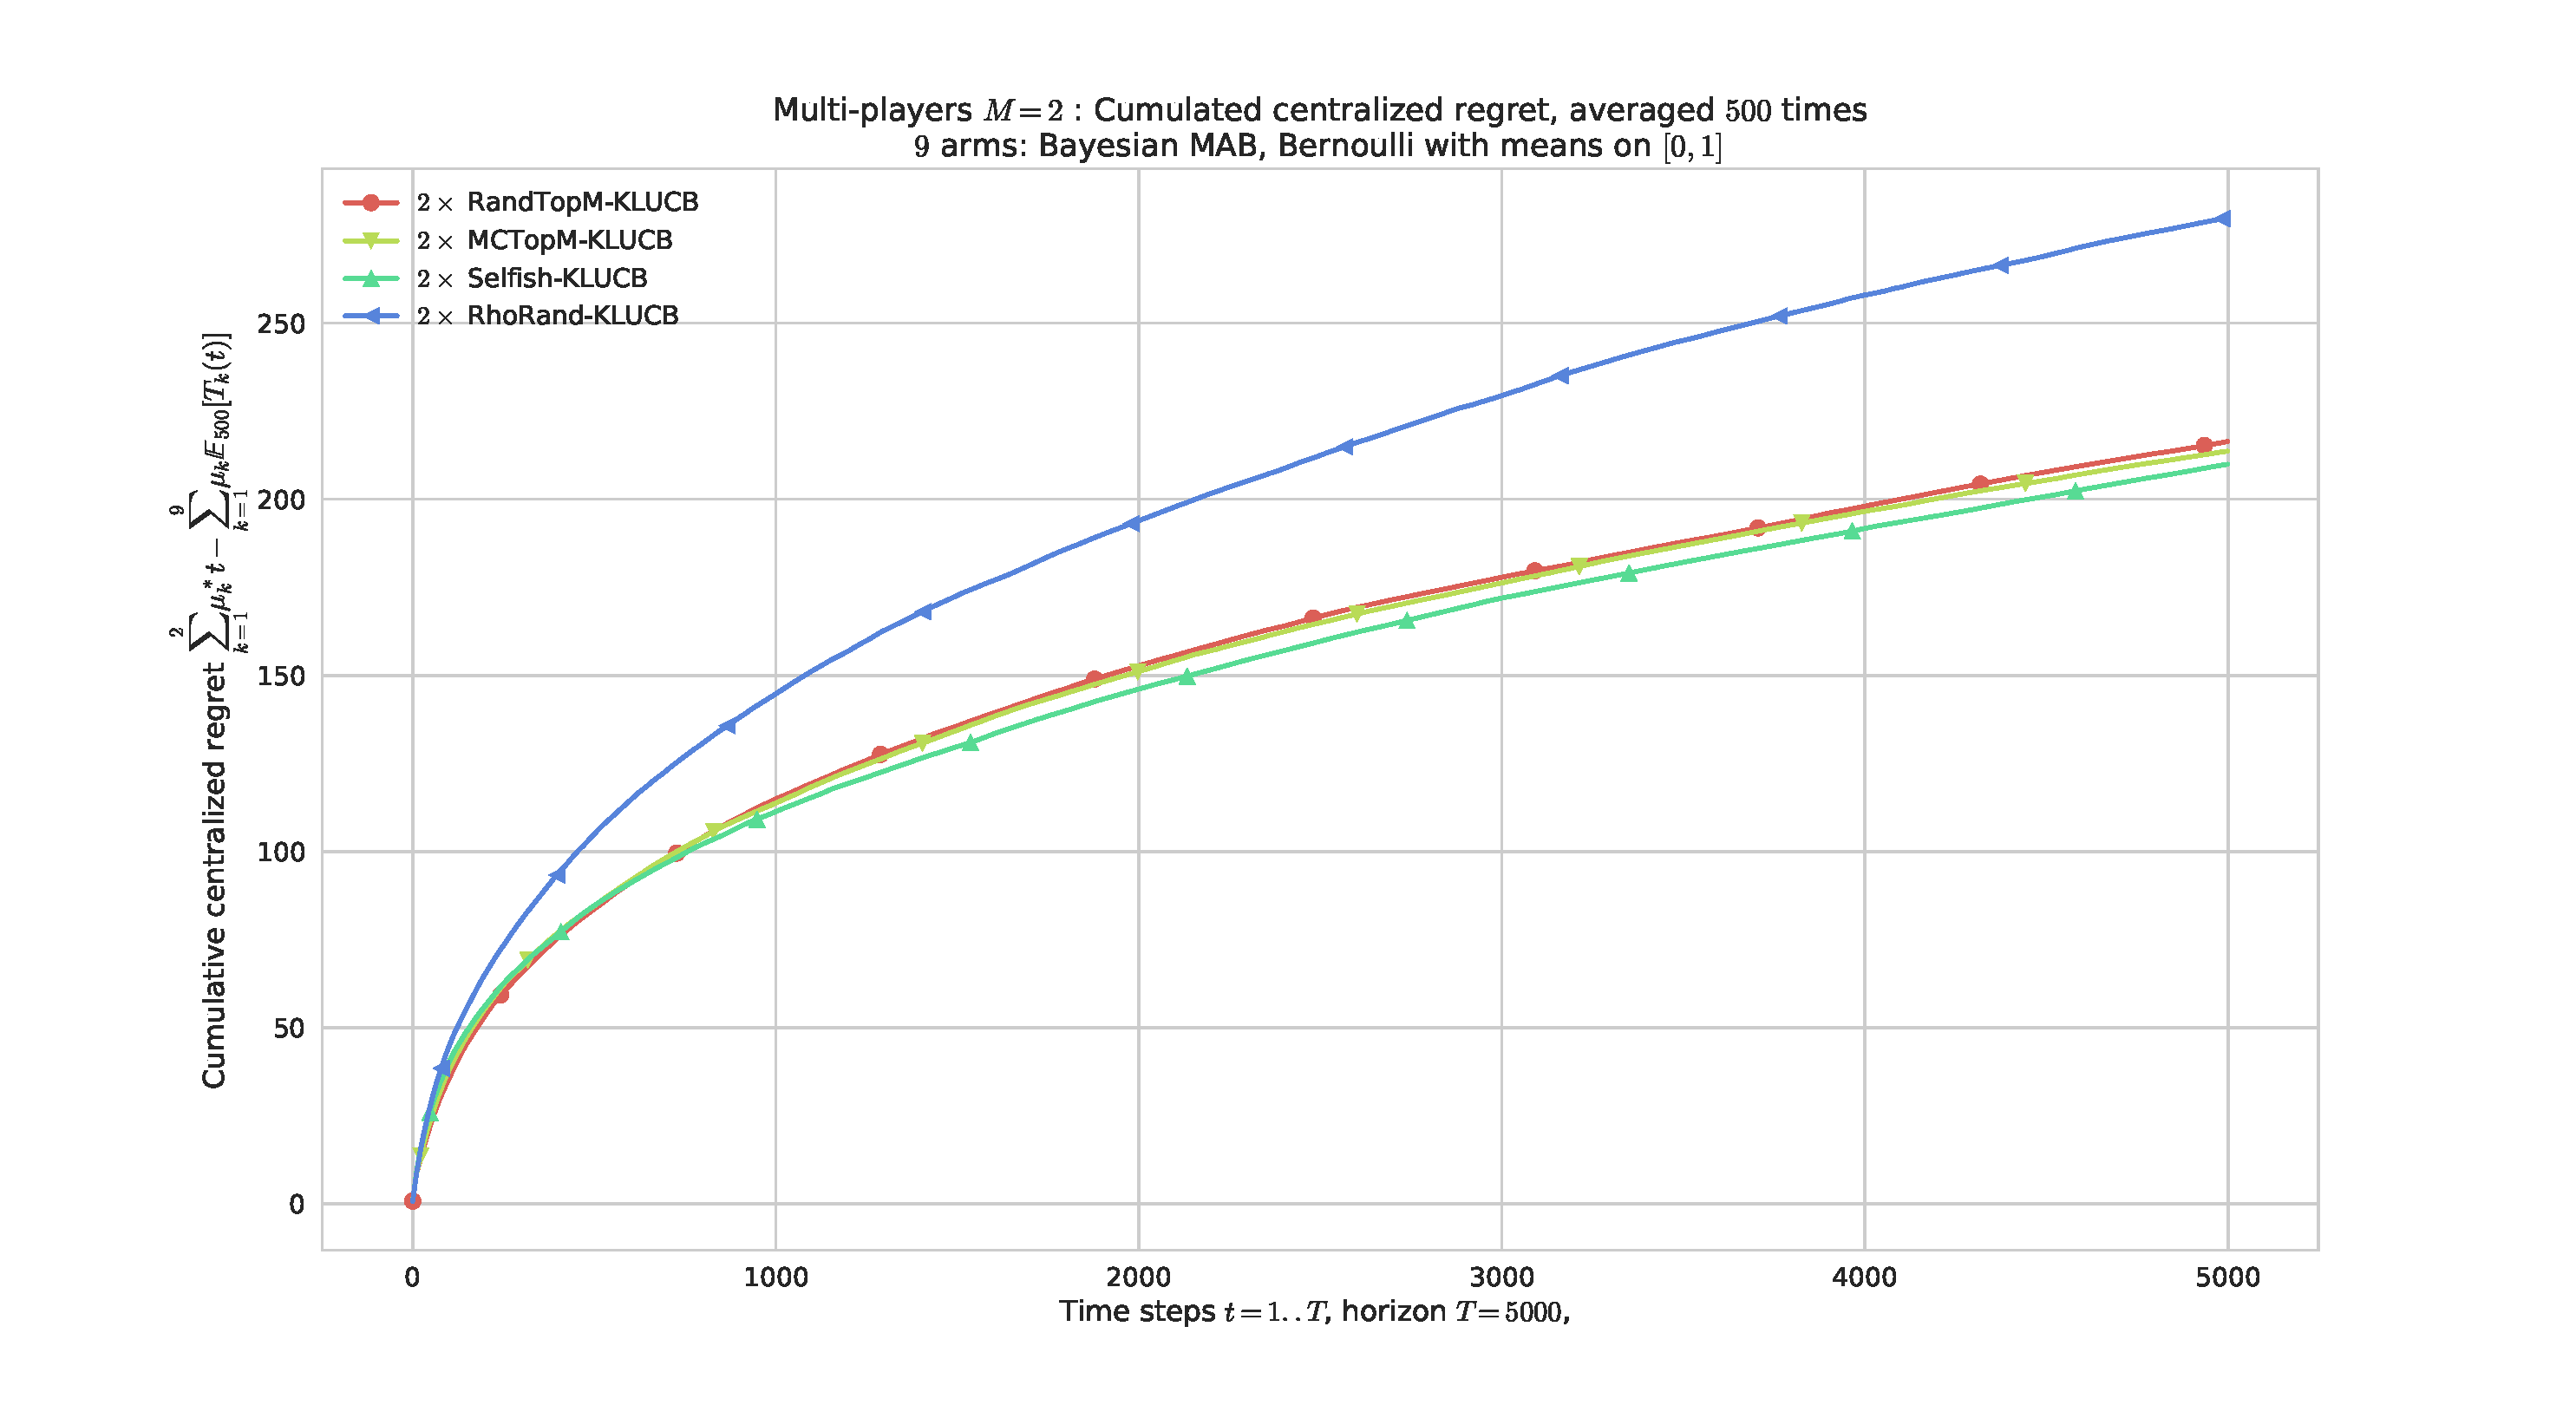
\includegraphics[width=1.00\textwidth]{MP__K9_M2_T5000_N500__4_algos/all_RegretCentralized____env1-1_3251433209347345969.pdf}
  % \end{subfigure}
  % % ~
  % \begin{subfigure}[!h]{0.49\textwidth}
    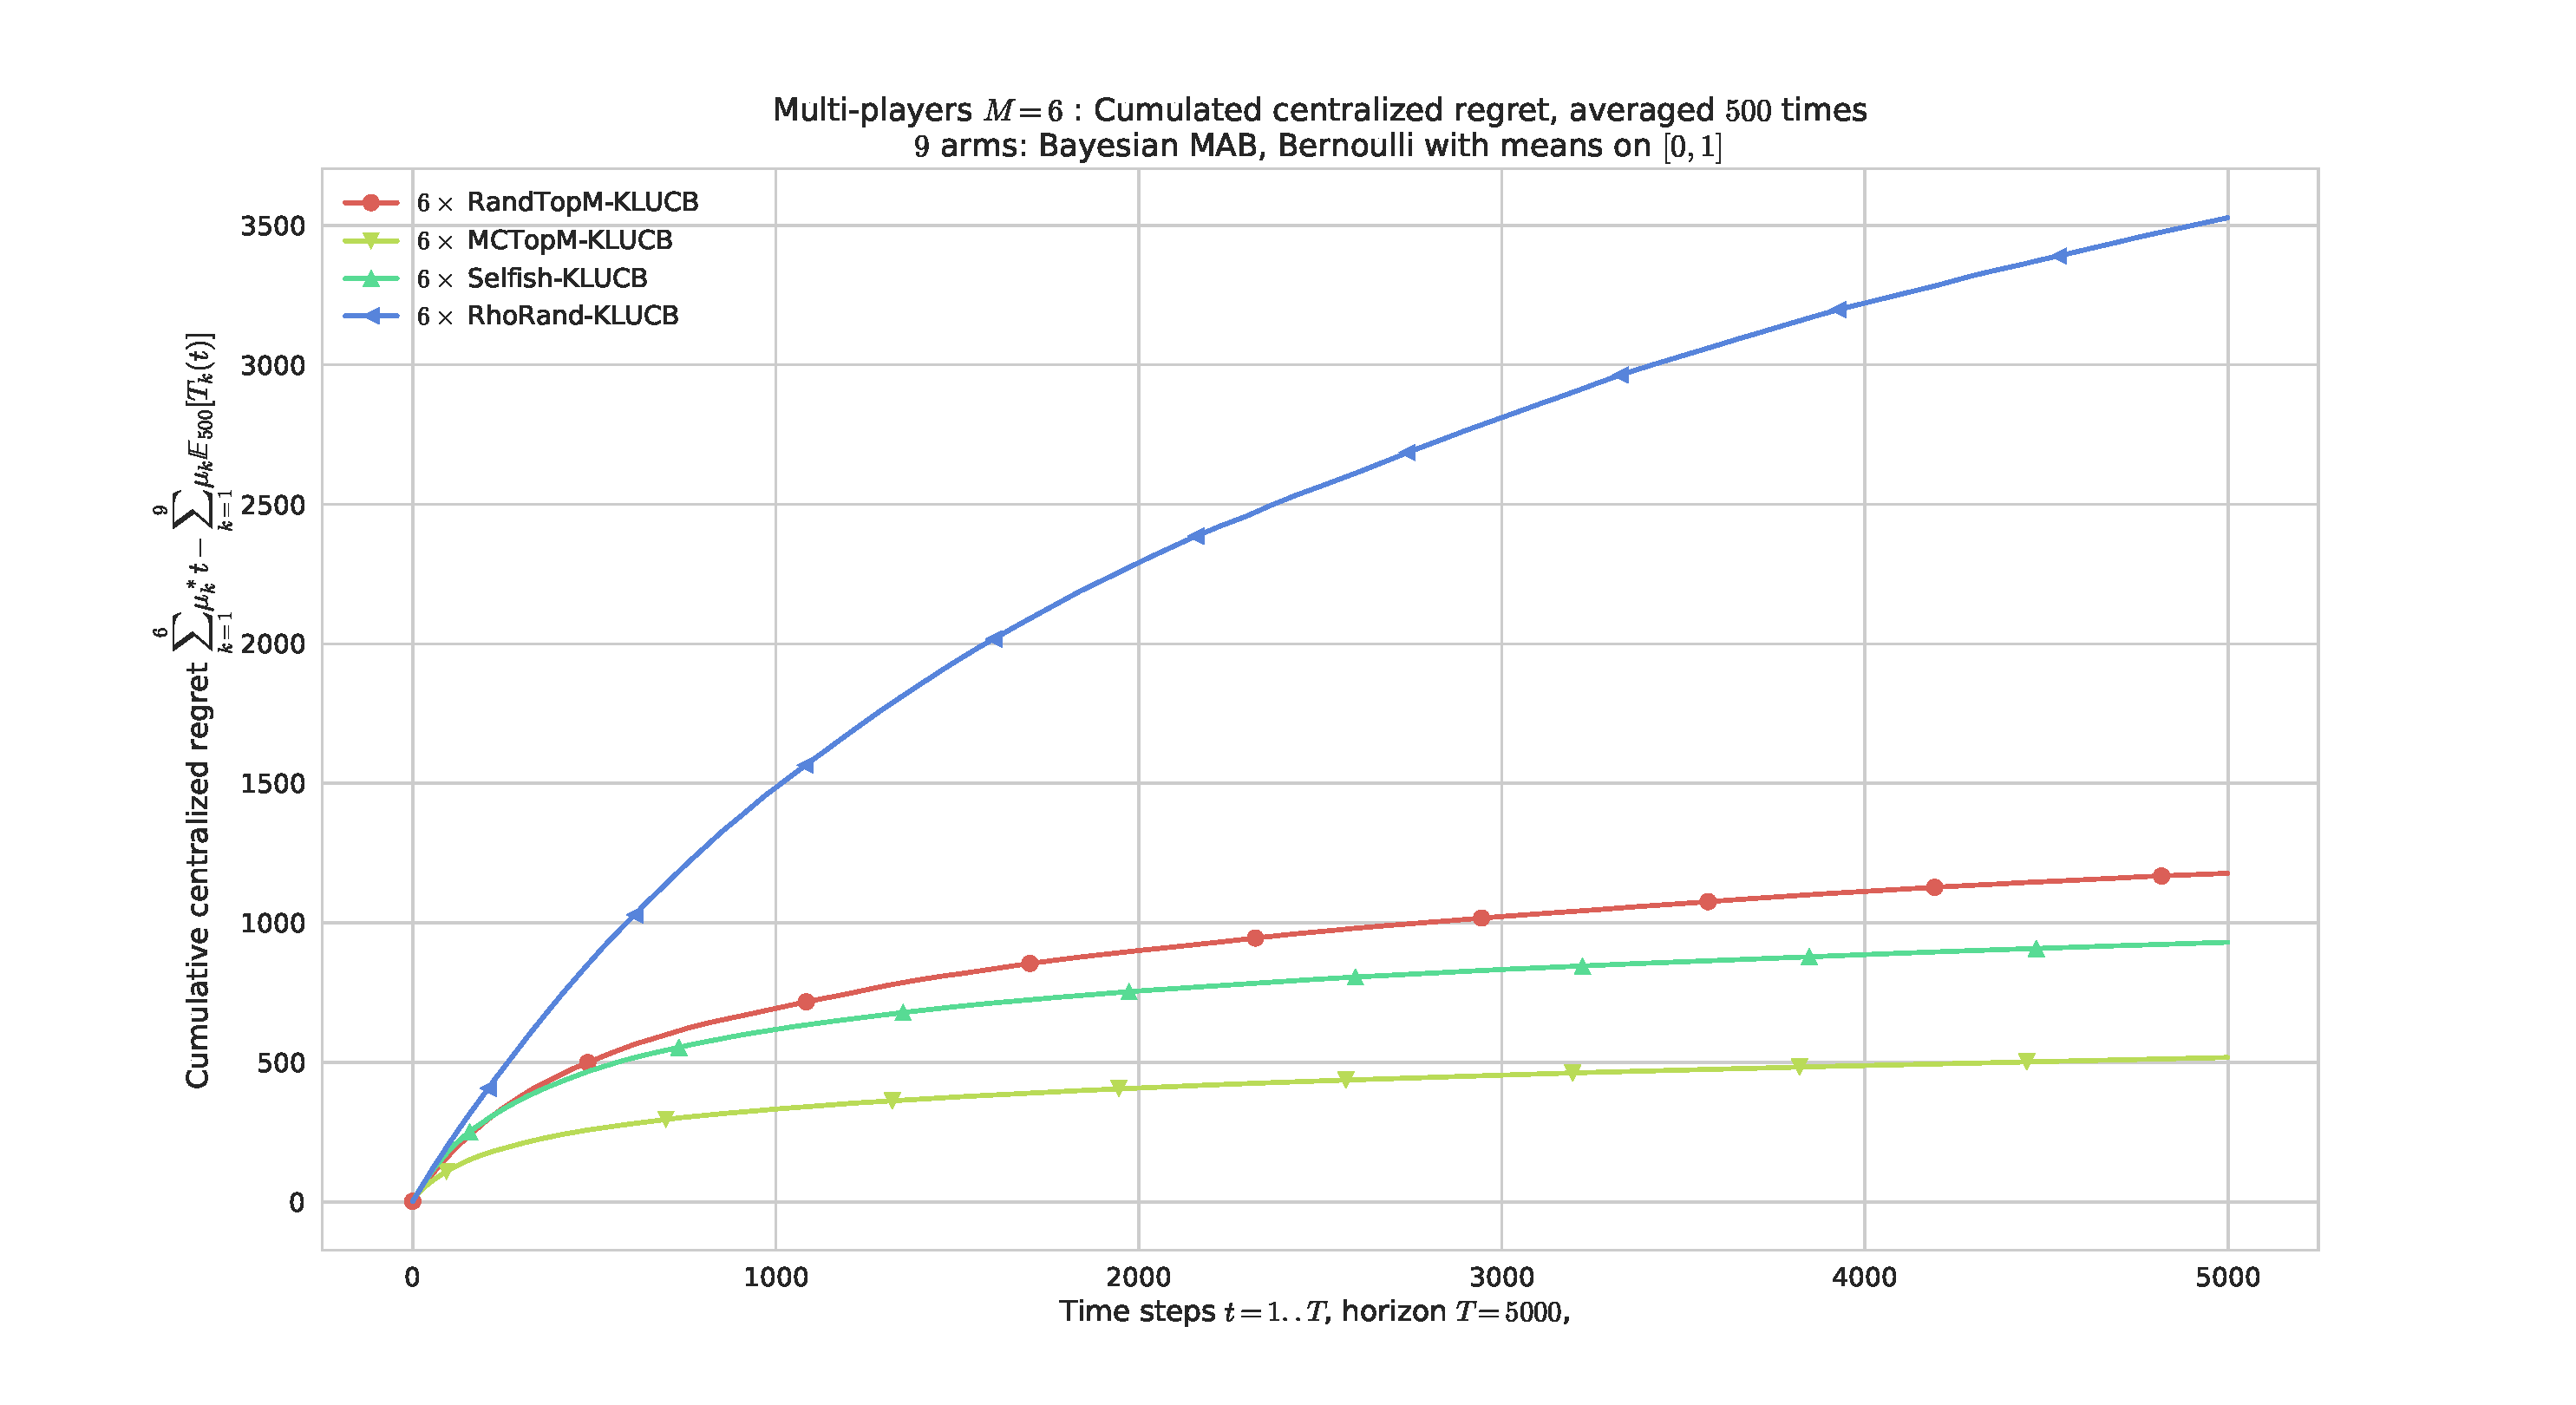
\includegraphics[width=1.10\textwidth]{MP__K9_M6_T5000_N500__4_algos/all_RegretCentralized____env1-1_8318947830261751207.pdf}
  % \end{subfigure}
  \caption[Regret for $M=6$ players, $K=9$ arms, horizon $T=5000$, against $500$ problems $\boldsymbol{\mu}$ uniformly sampled]{Regret for $M=6$ players, $K=9$ arms, horizon $T=5000$, against $500$ problems $\boldsymbol{\mu}$ uniformly sampled in $[0,1]^K$. \rhoRand{} (top \textcolor{blue}{blue} curve) is outperformed by the other algorithms (and the gain increases with $M$). \MCTopM{} (bottom \textcolor{gold}{yellow}) outperforms all the other algorithms is most cases.}
  % \label{fig:5:MP__K9_M2-6_T5000_N500__4_algos__all_RegretCentralized__BayesianProblems}
  \label{fig:5:MP__K9_M6_T5000_N500__4_algos__all_RegretCentralized__BayesianProblems}
  % \vspace*{-15pt}  % XXX remove if problem
\end{figure}



% Dynamic settings, when $M$ can change in time,
% were considered in the analysis of both
In the presence of sensing (observation model \modeldeux), we also compared our algorithms to  %multi-player multi-armed bandits algorithms
with \MEGA{} \citep{Avner15} and \MusicalChair{} \citep{Rosenski16}. Yet these two algorithms were found hard to use efficiently in practice and we show in
% that were also proposed
%
Figure~\ref{fig:5:MP__K9_M3_T123456_N100__8_algos} that they perform poorly in comparison to \rhoRand, \RandTopM{} and \MCTopM.
%
\MEGA{} needs a careful tuning of \emph{five} parameters ($c$, $d$, $p_0$, $\alpha$ and $\beta$) to attain reasonable performances. No good guideline for tuning them is provided and using cross validation, as suggested,
can be considered out of the scope of online sequential learning.
%In practice, on a fixed instance, the authors do not indicate how to select the parameters, even with a perfect knowledge of the parameters ($\boldsymbol{\mu}$ and $T$).
%
\MusicalChair{} consists of a random exploration phase of length $T_0$ after which the players quickly converge to orthogonal strategies targeting the $M$ best arms. With probability $1-\delta$, its regret is proved to be ``constant'' (of order $\log(1/\delta)$). The theoretical minimal value for $T_0$ depends on $\delta$, on the horizon $T$ and on a lower bound $\epsilon$ on the gap $\Delta = \mu^*_M - \mu^*_{M+1}$, and the practical tuning is hard too. %% which are both unavailable in our setting.



\begin{figure}[!h]
  \centering
  % \begin{subfigure}[!h]{0.85\textwidth}
    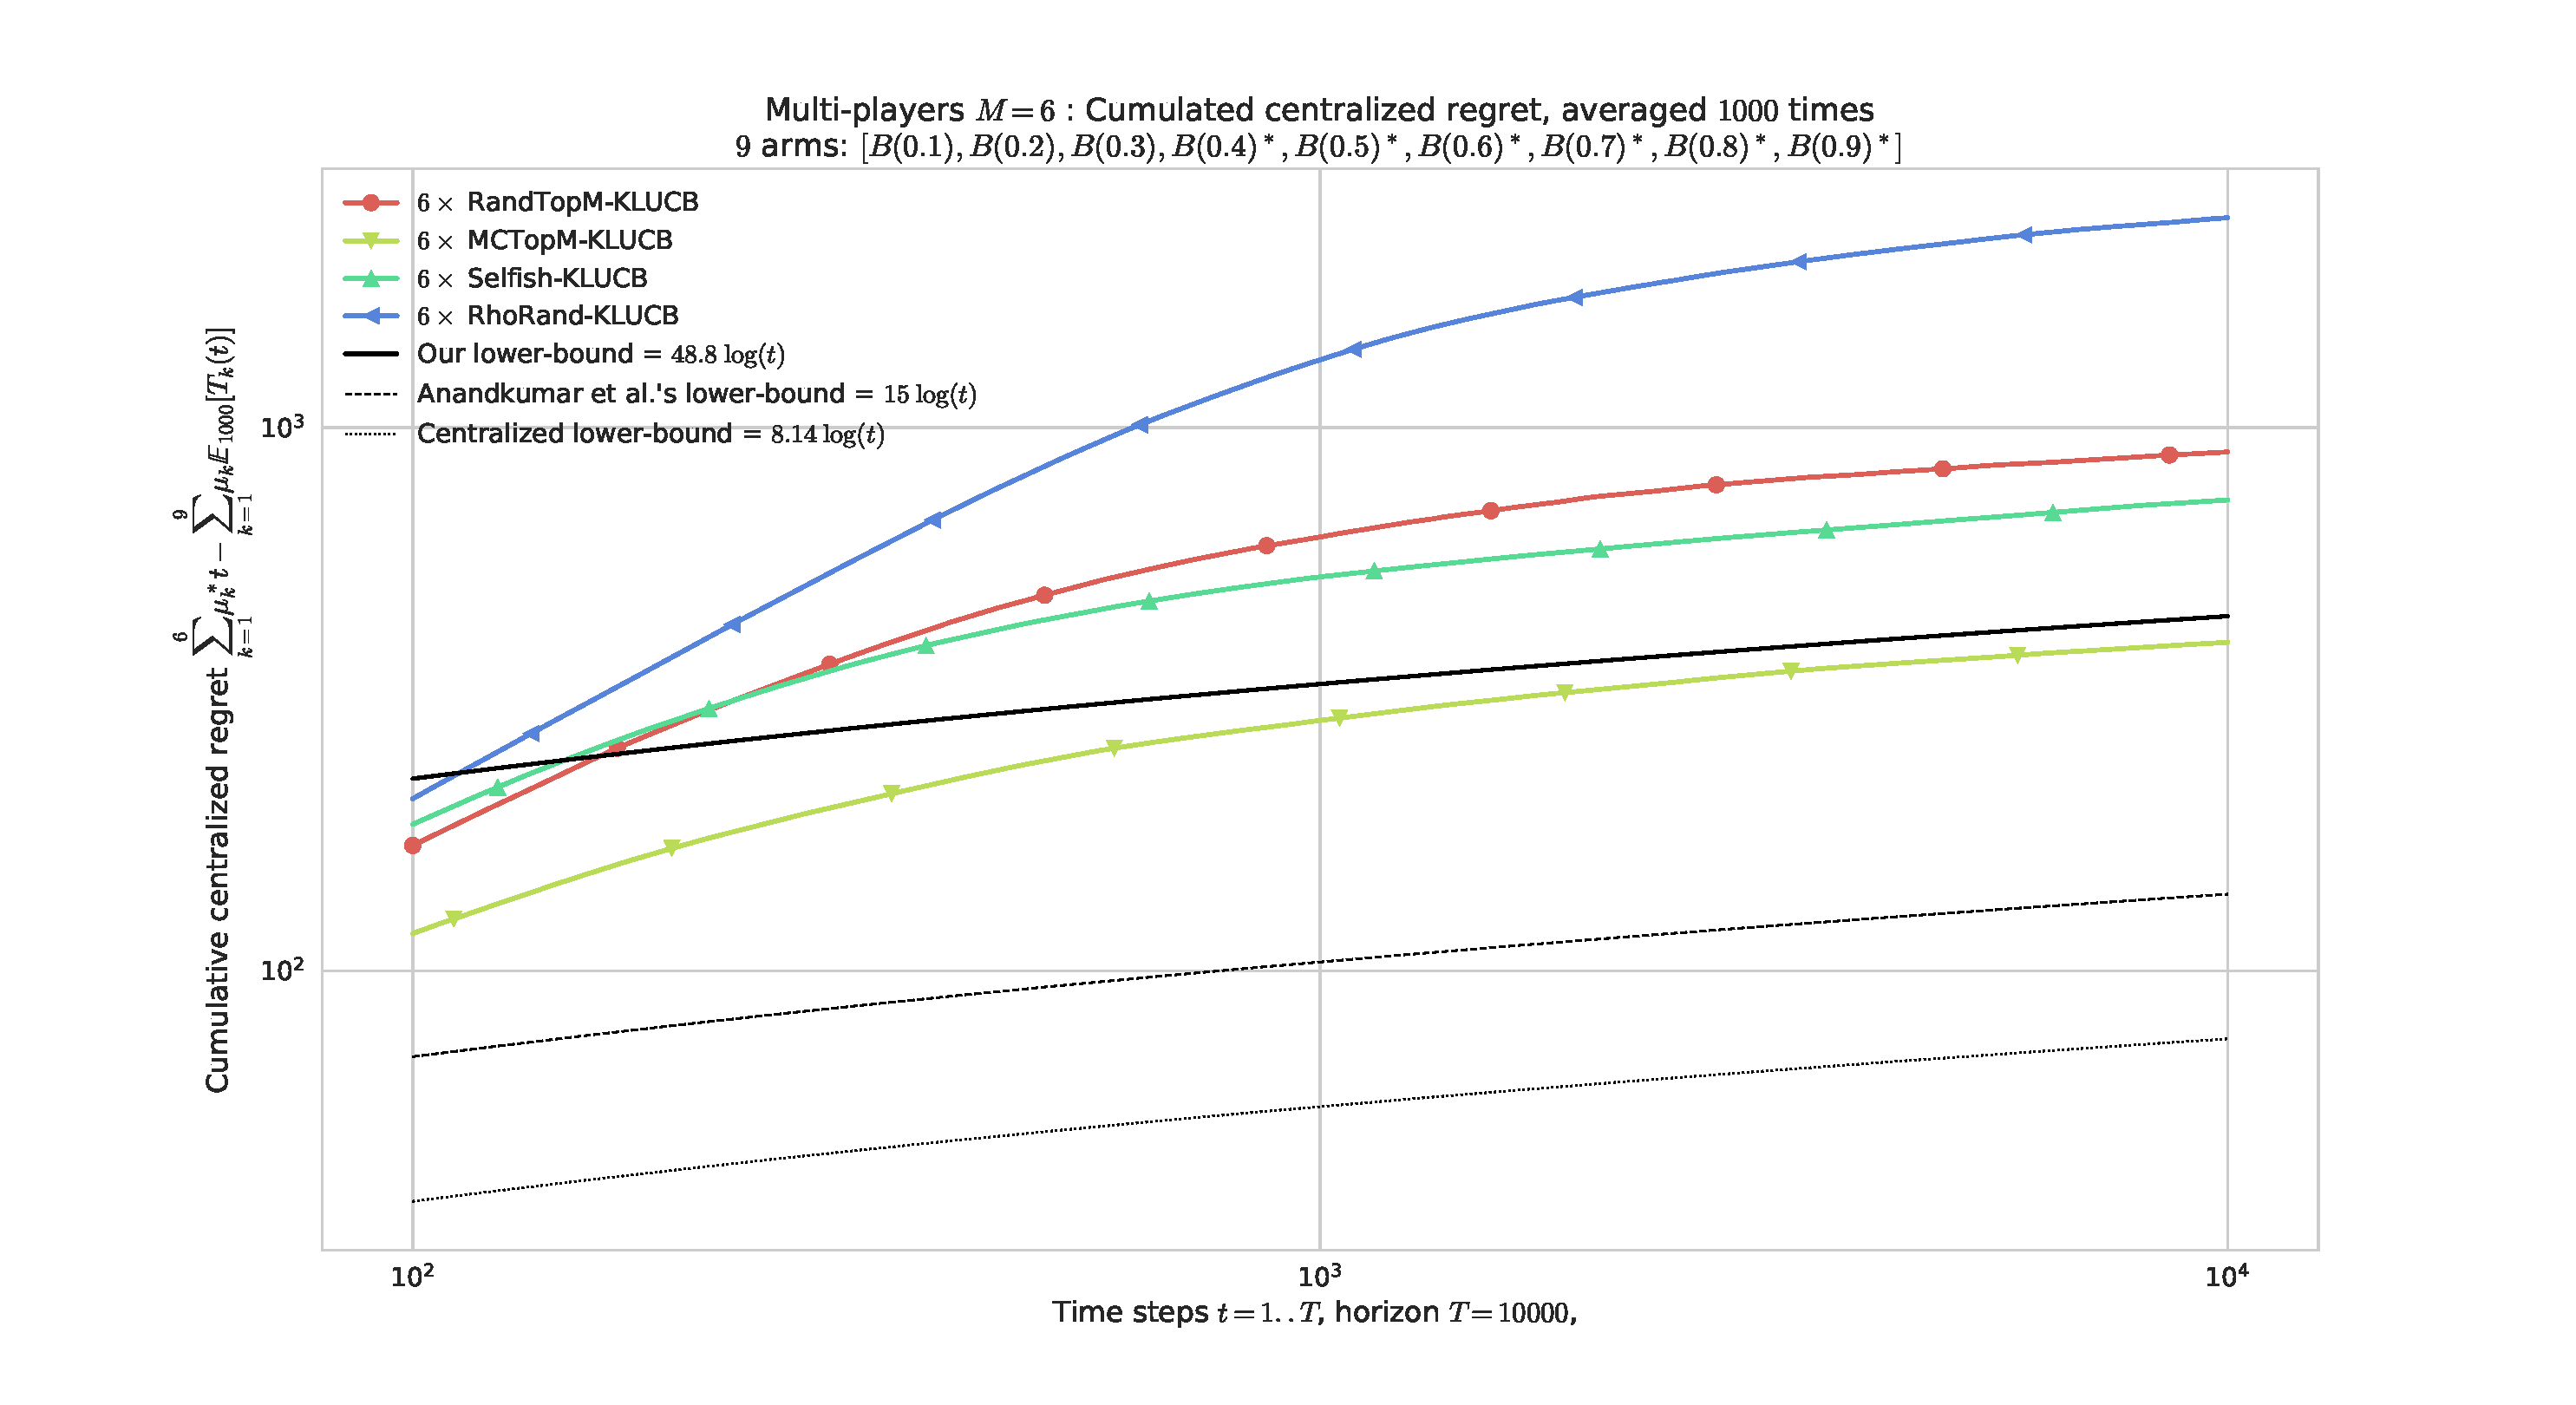
\includegraphics[width=1.10\textwidth]{MP__K9_M6_T10000_N1000__4_algos/all_RegretCentralized_loglog____env1-1_8200873569864822246.pdf}
  % \end{subfigure}
  % ~
  % \begin{subfigure}[!h]{0.85\textwidth}
    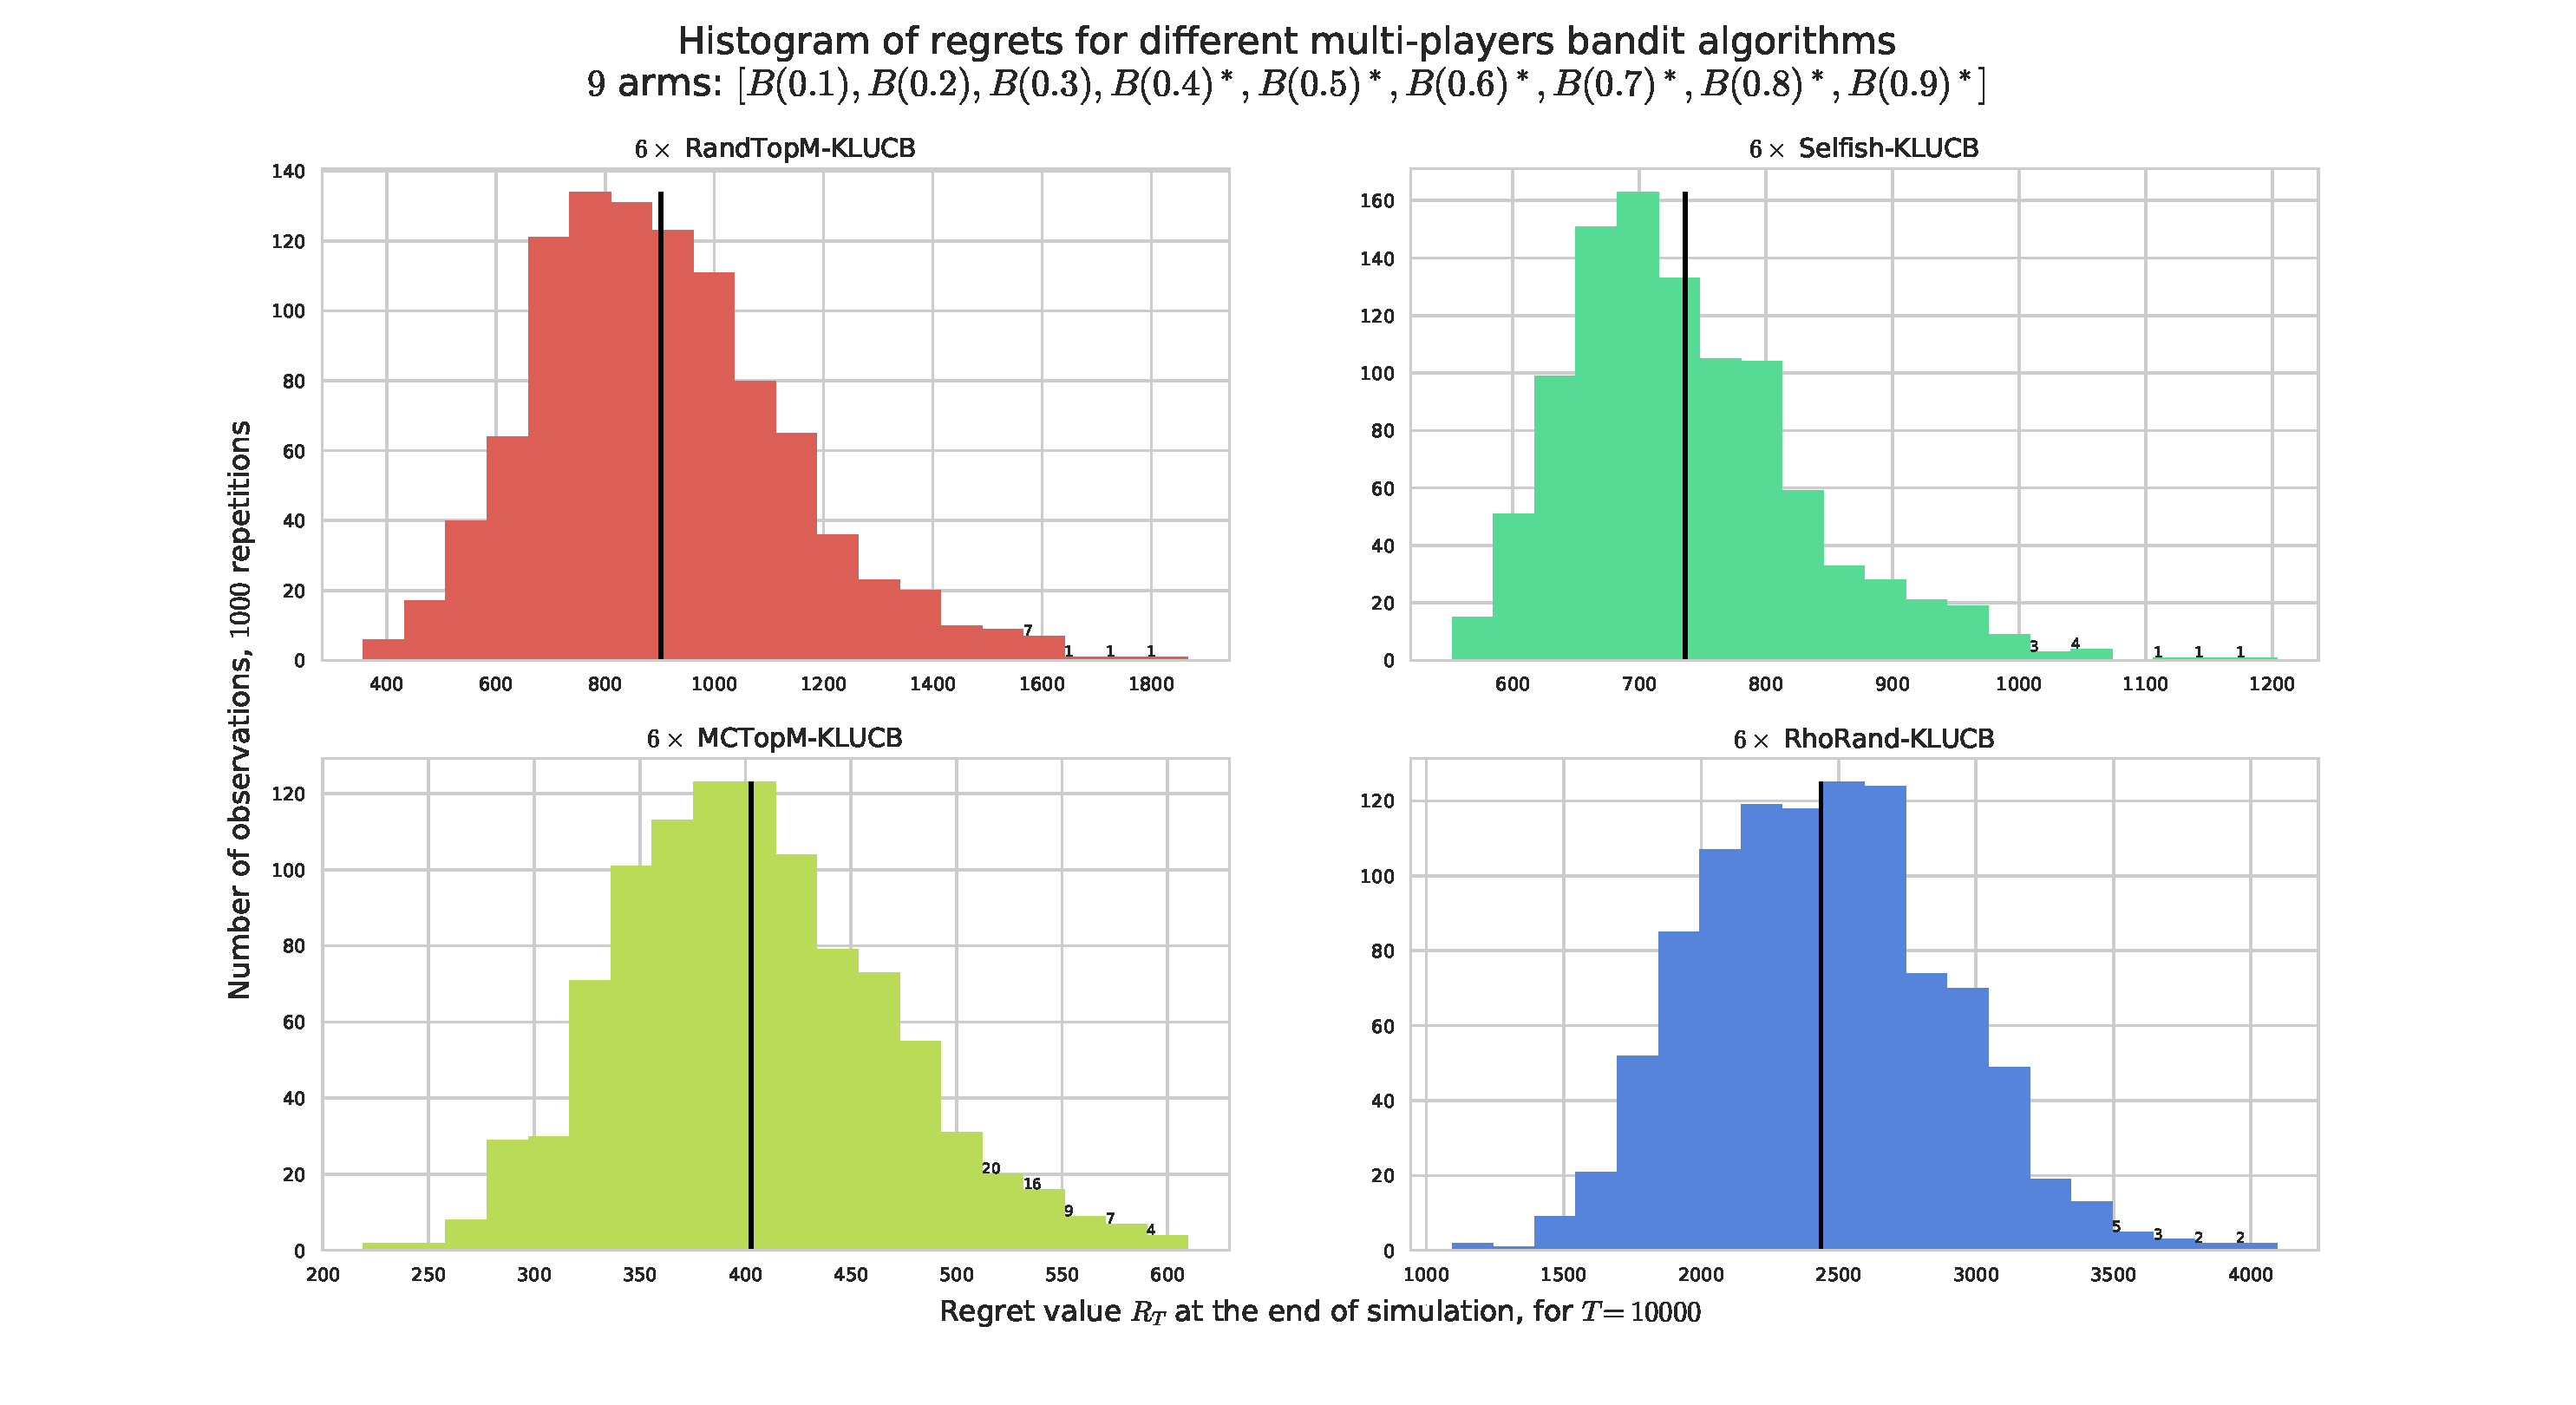
\includegraphics[width=1.10\textwidth]{MP__K9_M6_T10000_N1000__4_algos/all_HistogramsRegret____env1-1_8200873569864822246.pdf}
  % \end{subfigure}
  \caption[Regret for $M=6$ players for $K=9$ arms, horizon $T=5000$, for $1000$ repetitions on a fixed problem]{Regret (in log-log scale), for $M=6$ players for $K=9$ arms, horizon $T=5000$, for $1000$ repetitions on problem $\boldsymbol{\mu}=[0.1,\dots,0.9]$. \RandTopM{} (\textcolor{gold}{yellow} curve) outperforms \Selfish{} (\textcolor{darkgreen}{green}), both clearly outperform \rhoRand. The regret of \MCTopM{} is logarithmic, empirically with the same slope as the lower bound. The $x$ axis on the regret histograms have different scale for each algorithm.}
  \label{fig:5:MP__K9_M6_T10000_N1000__4_algos}
\end{figure}




\begin{figure}[!h]
  \centering
  % \begin{subfigure}[!h]{0.85\textwidth}
      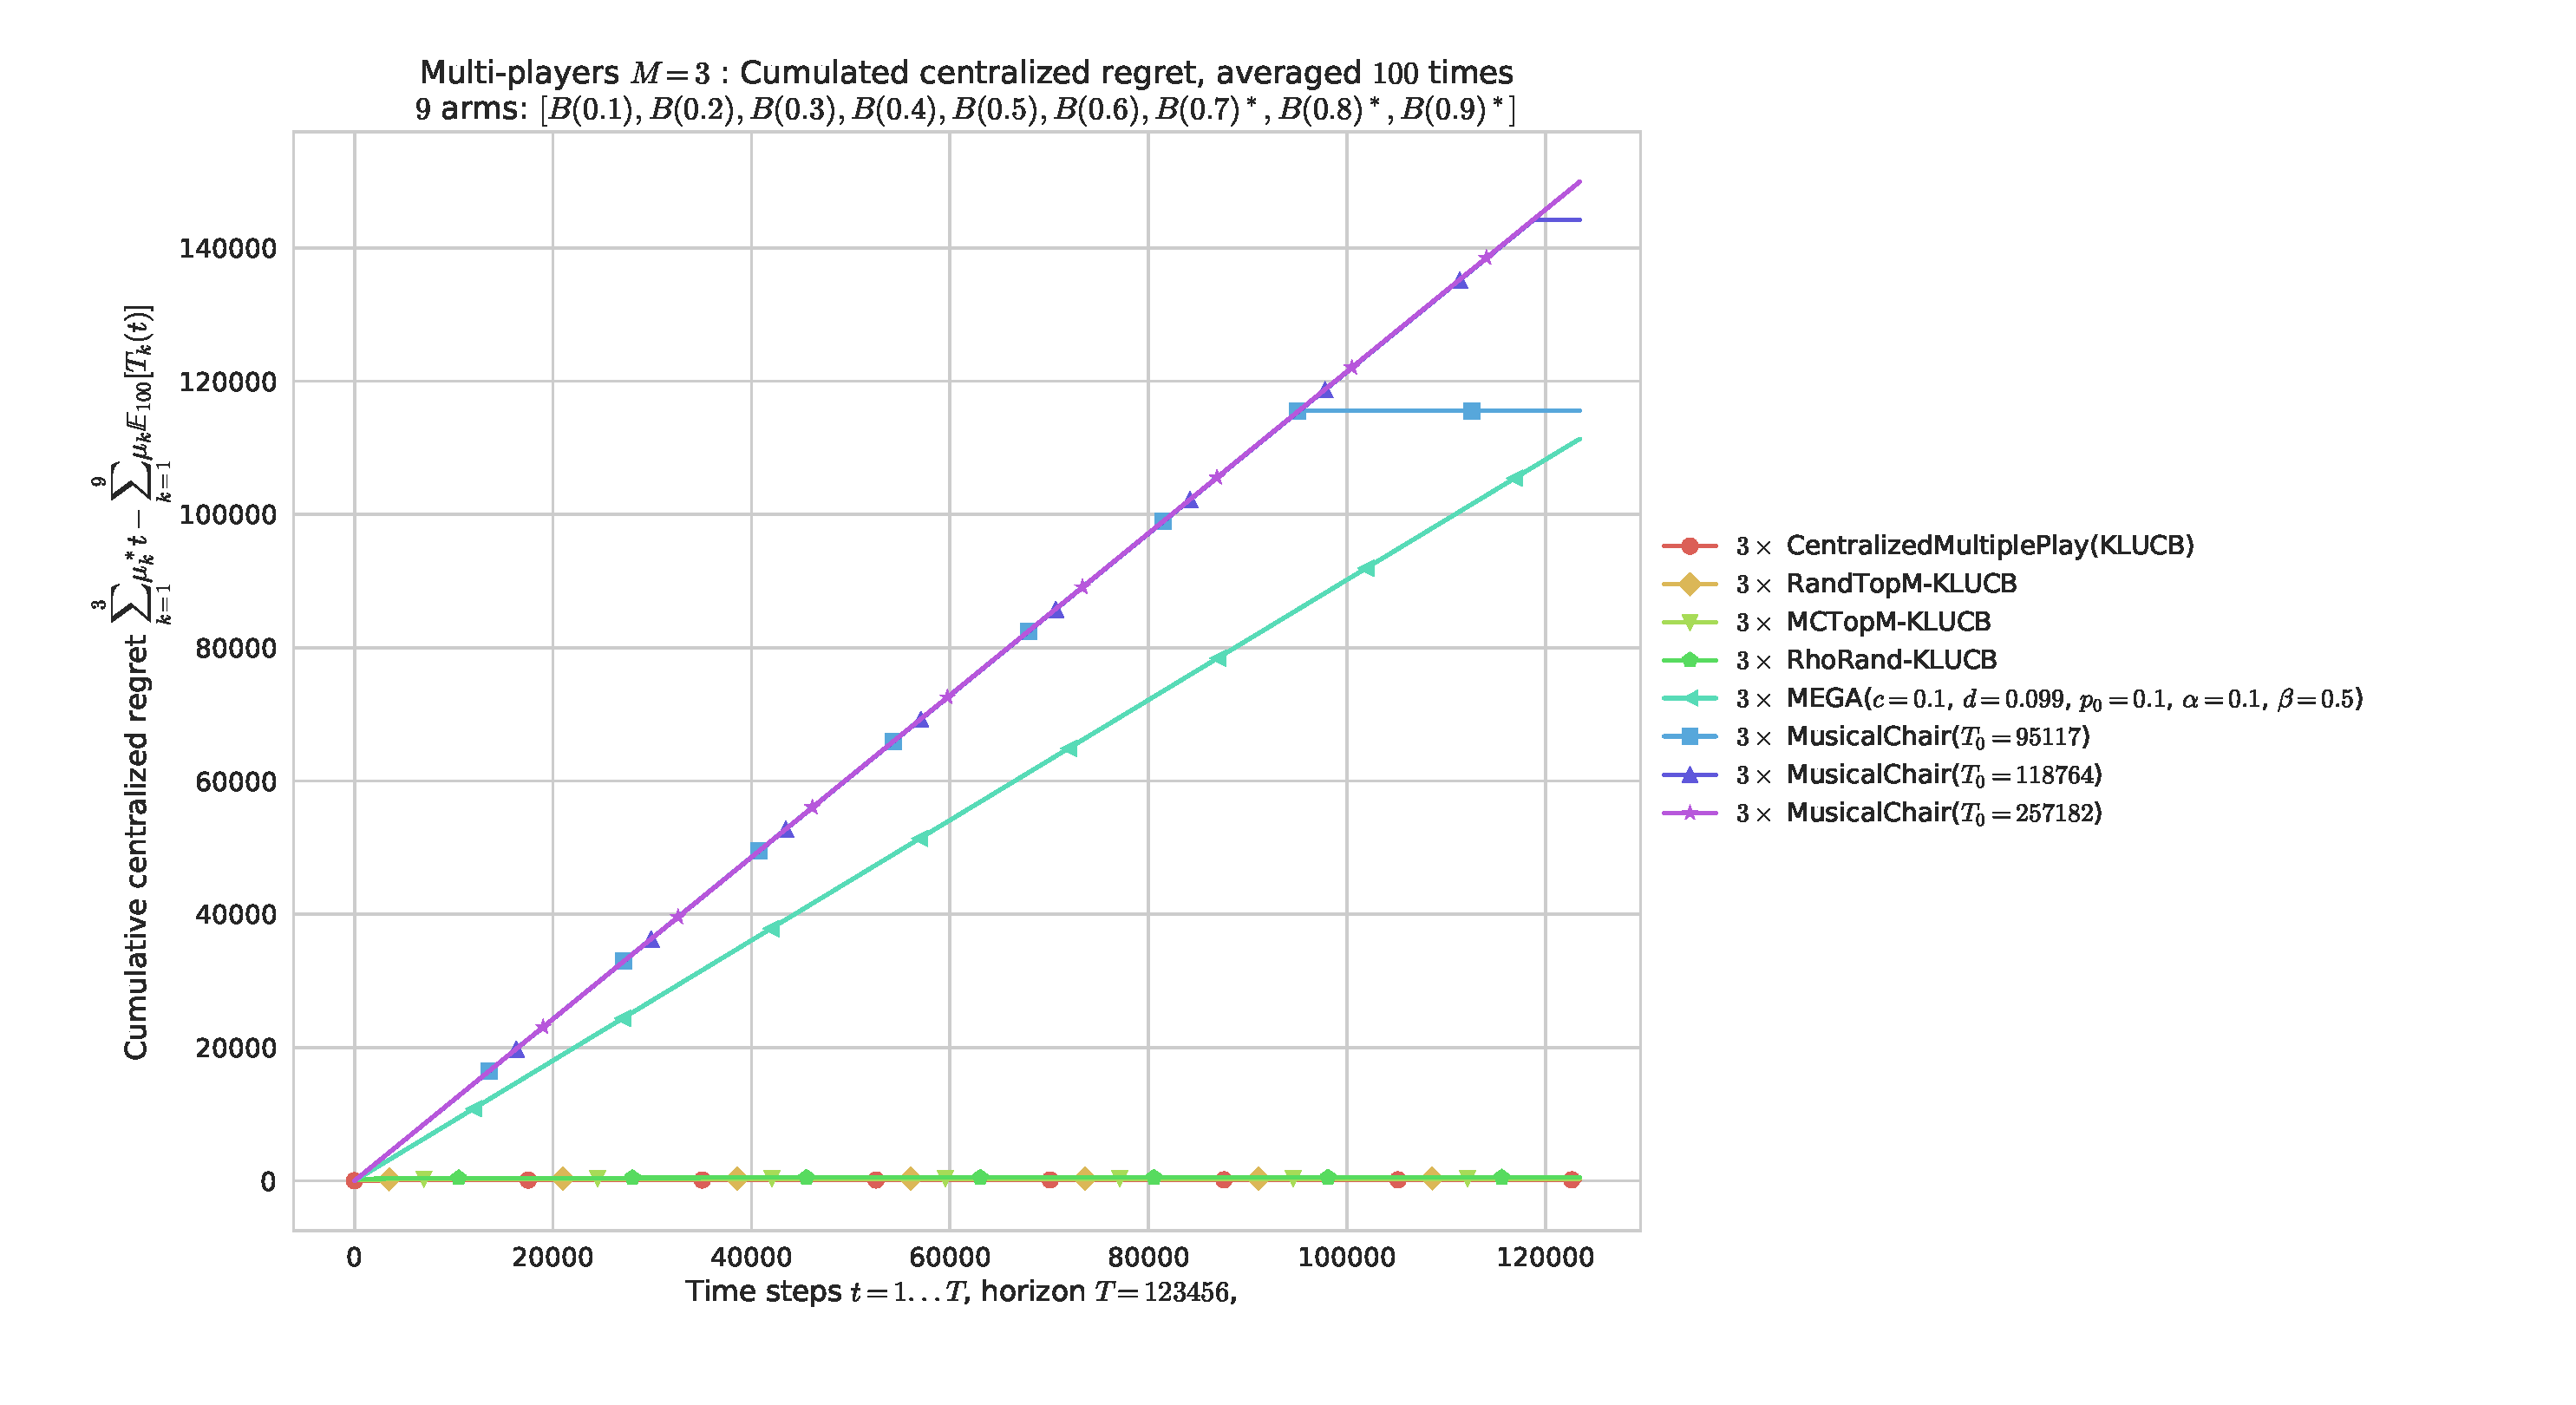
\includegraphics[width=1.00\textwidth]{MP__K9_M3_T123456_N100__8_algos/all_RegretCentralized____env1-1_7803645526012310577.pdf}
  % \end{subfigure}
  % ~
  % \begin{subfigure}[!h]{0.85\textwidth}
      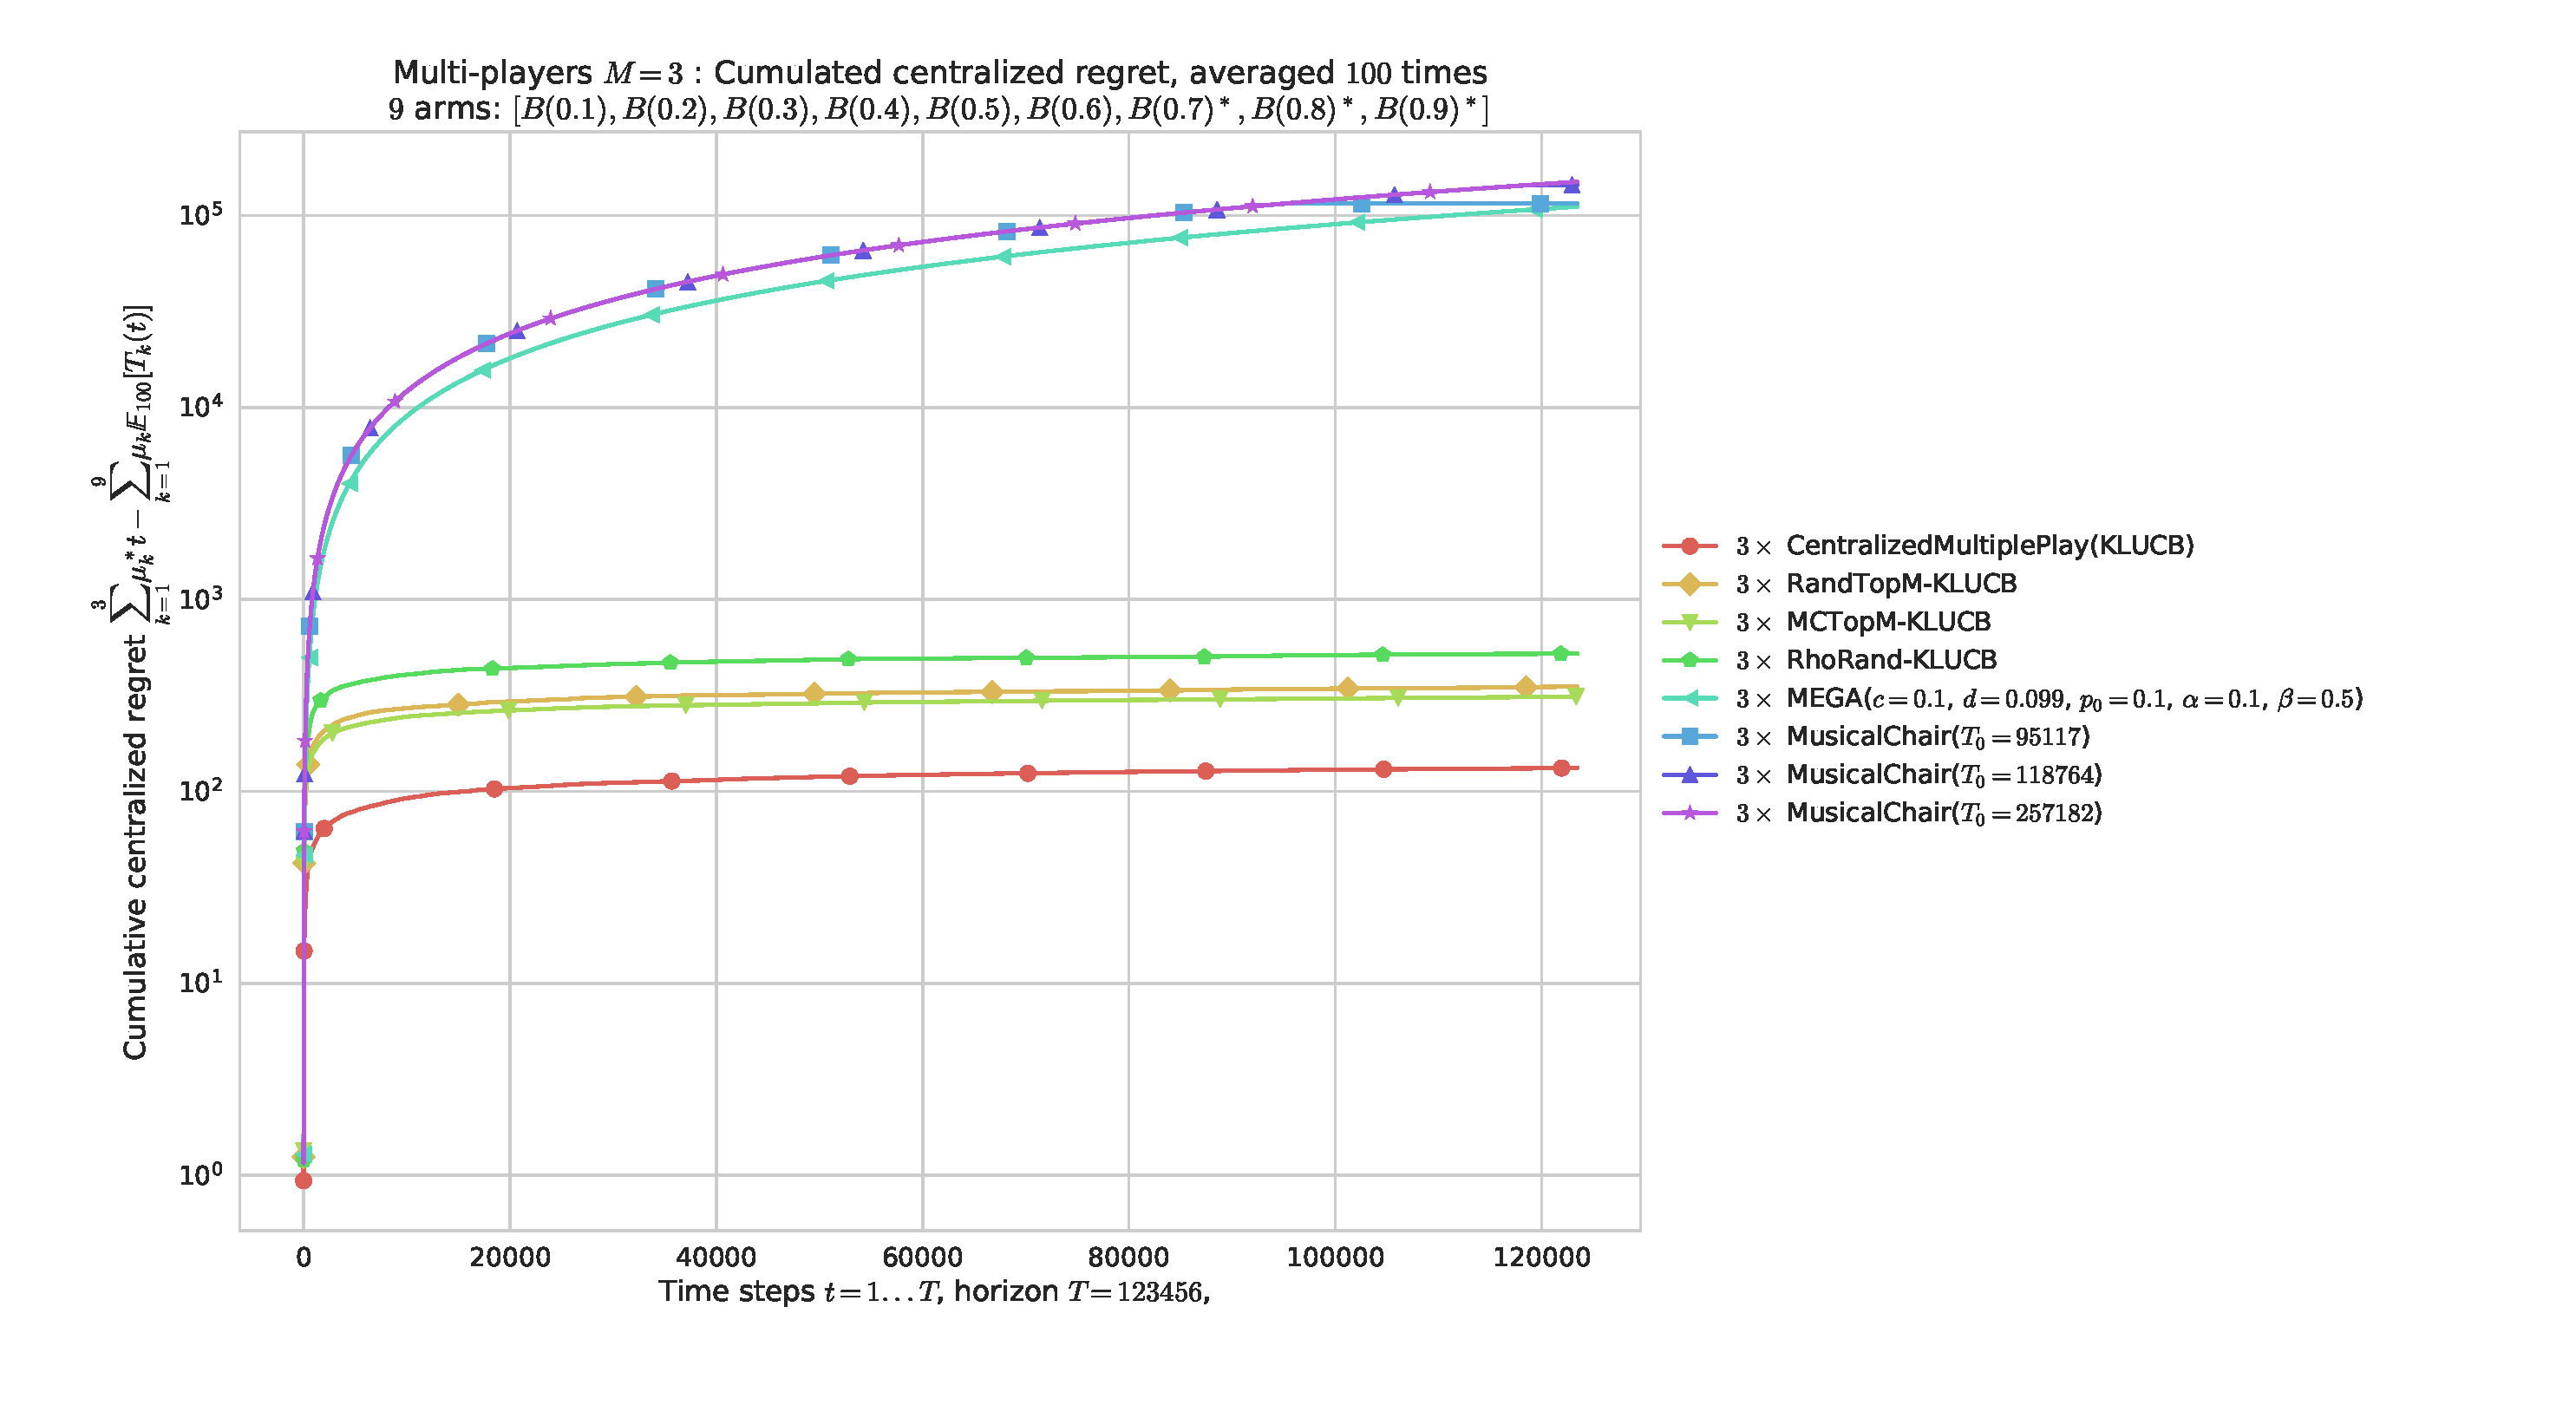
\includegraphics[width=1.00\textwidth]{MP__K9_M3_T123456_N100__8_algos/all_RegretCentralized_semilogy____env1-1_7803645526012310577.pdf}
  % \end{subfigure}
  \caption[Regret for $M=3$ players for $K=9$ arms, horizon $T=123456$, for $100$ repetitions on a fixed problem]{Regret (in log-$y$ scale on the right) for $M=3$ players for $K=9$ arms, horizon $T=123456$, for $100$ repetitions on problem $\mu=[0.1,\dots,0.9]$. With a perfect knowledge on the gap ($\Delta=0.1$ here) and by using the parameters suggested from their respective articles, \MEGA{} and \MusicalChair{} perform badly in this simple setting, even with the knowledge of the horizon $T$ for \MusicalChair{}. The first two \MusicalChair{} instances use the optimal $T_0$ value from \cite{Rosenski16}, with $\varepsilon$ taken slightly smaller than the gap $\Delta$ ($\varepsilon=0.99 \Delta$), and respectively with $\delta=0.5$ and $\delta=0.1$, for which the regret can bounded with probability $0.5$ and $0.9$ respectively. The third instance uses the optimal $T_0$ corresponding to $\delta=1/T$, that is guaranteed to have an expected regret of order $\log(T)$.}
  \label{fig:5:MP__K9_M3_T123456_N100__8_algos}
\end{figure}

%
% Regular plots of centralized regrets
%
\begin{figure}[!h]
  \centering
  % \begin{subfigure}[!h]{0.49\textwidth}
      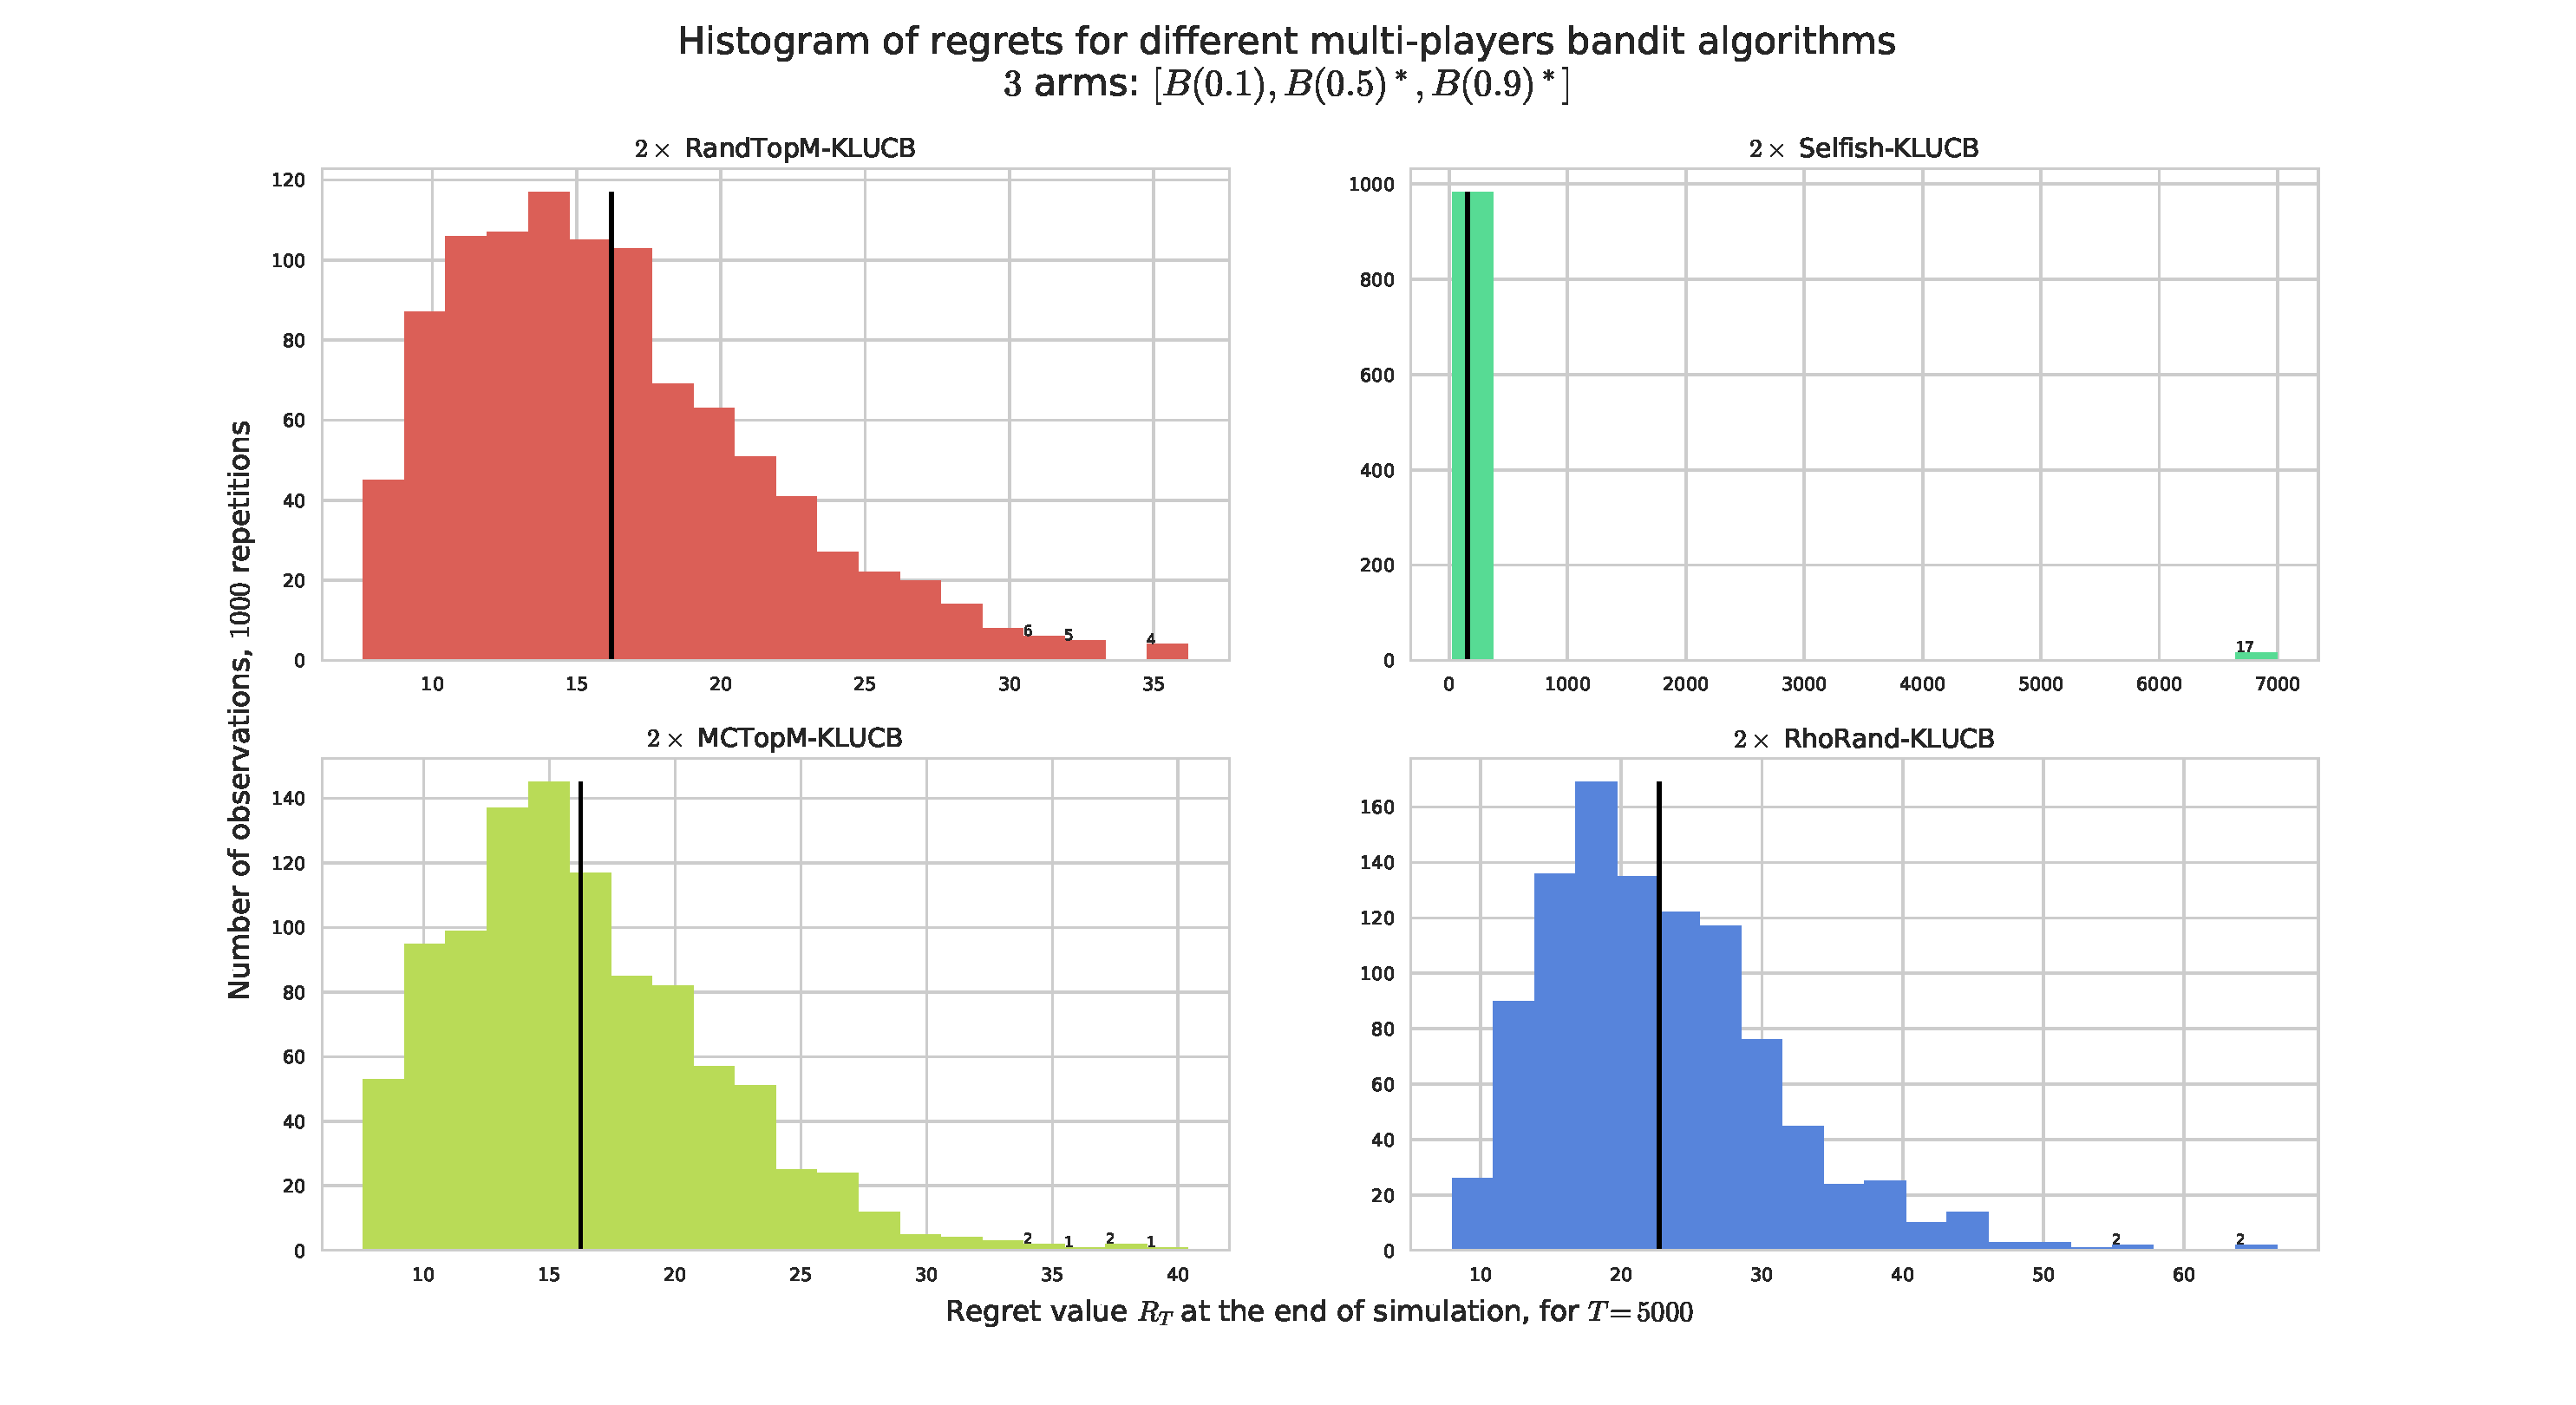
\includegraphics[width=1.00\textwidth]{MP__K3_M2_T5000_N1000__4_algos/all_HistogramsRegret____env1-1_5016720151160452442.pdf}
  % \end{subfigure}
  % % ~
  % \begin{subfigure}[!h]{0.49\textwidth}
  %   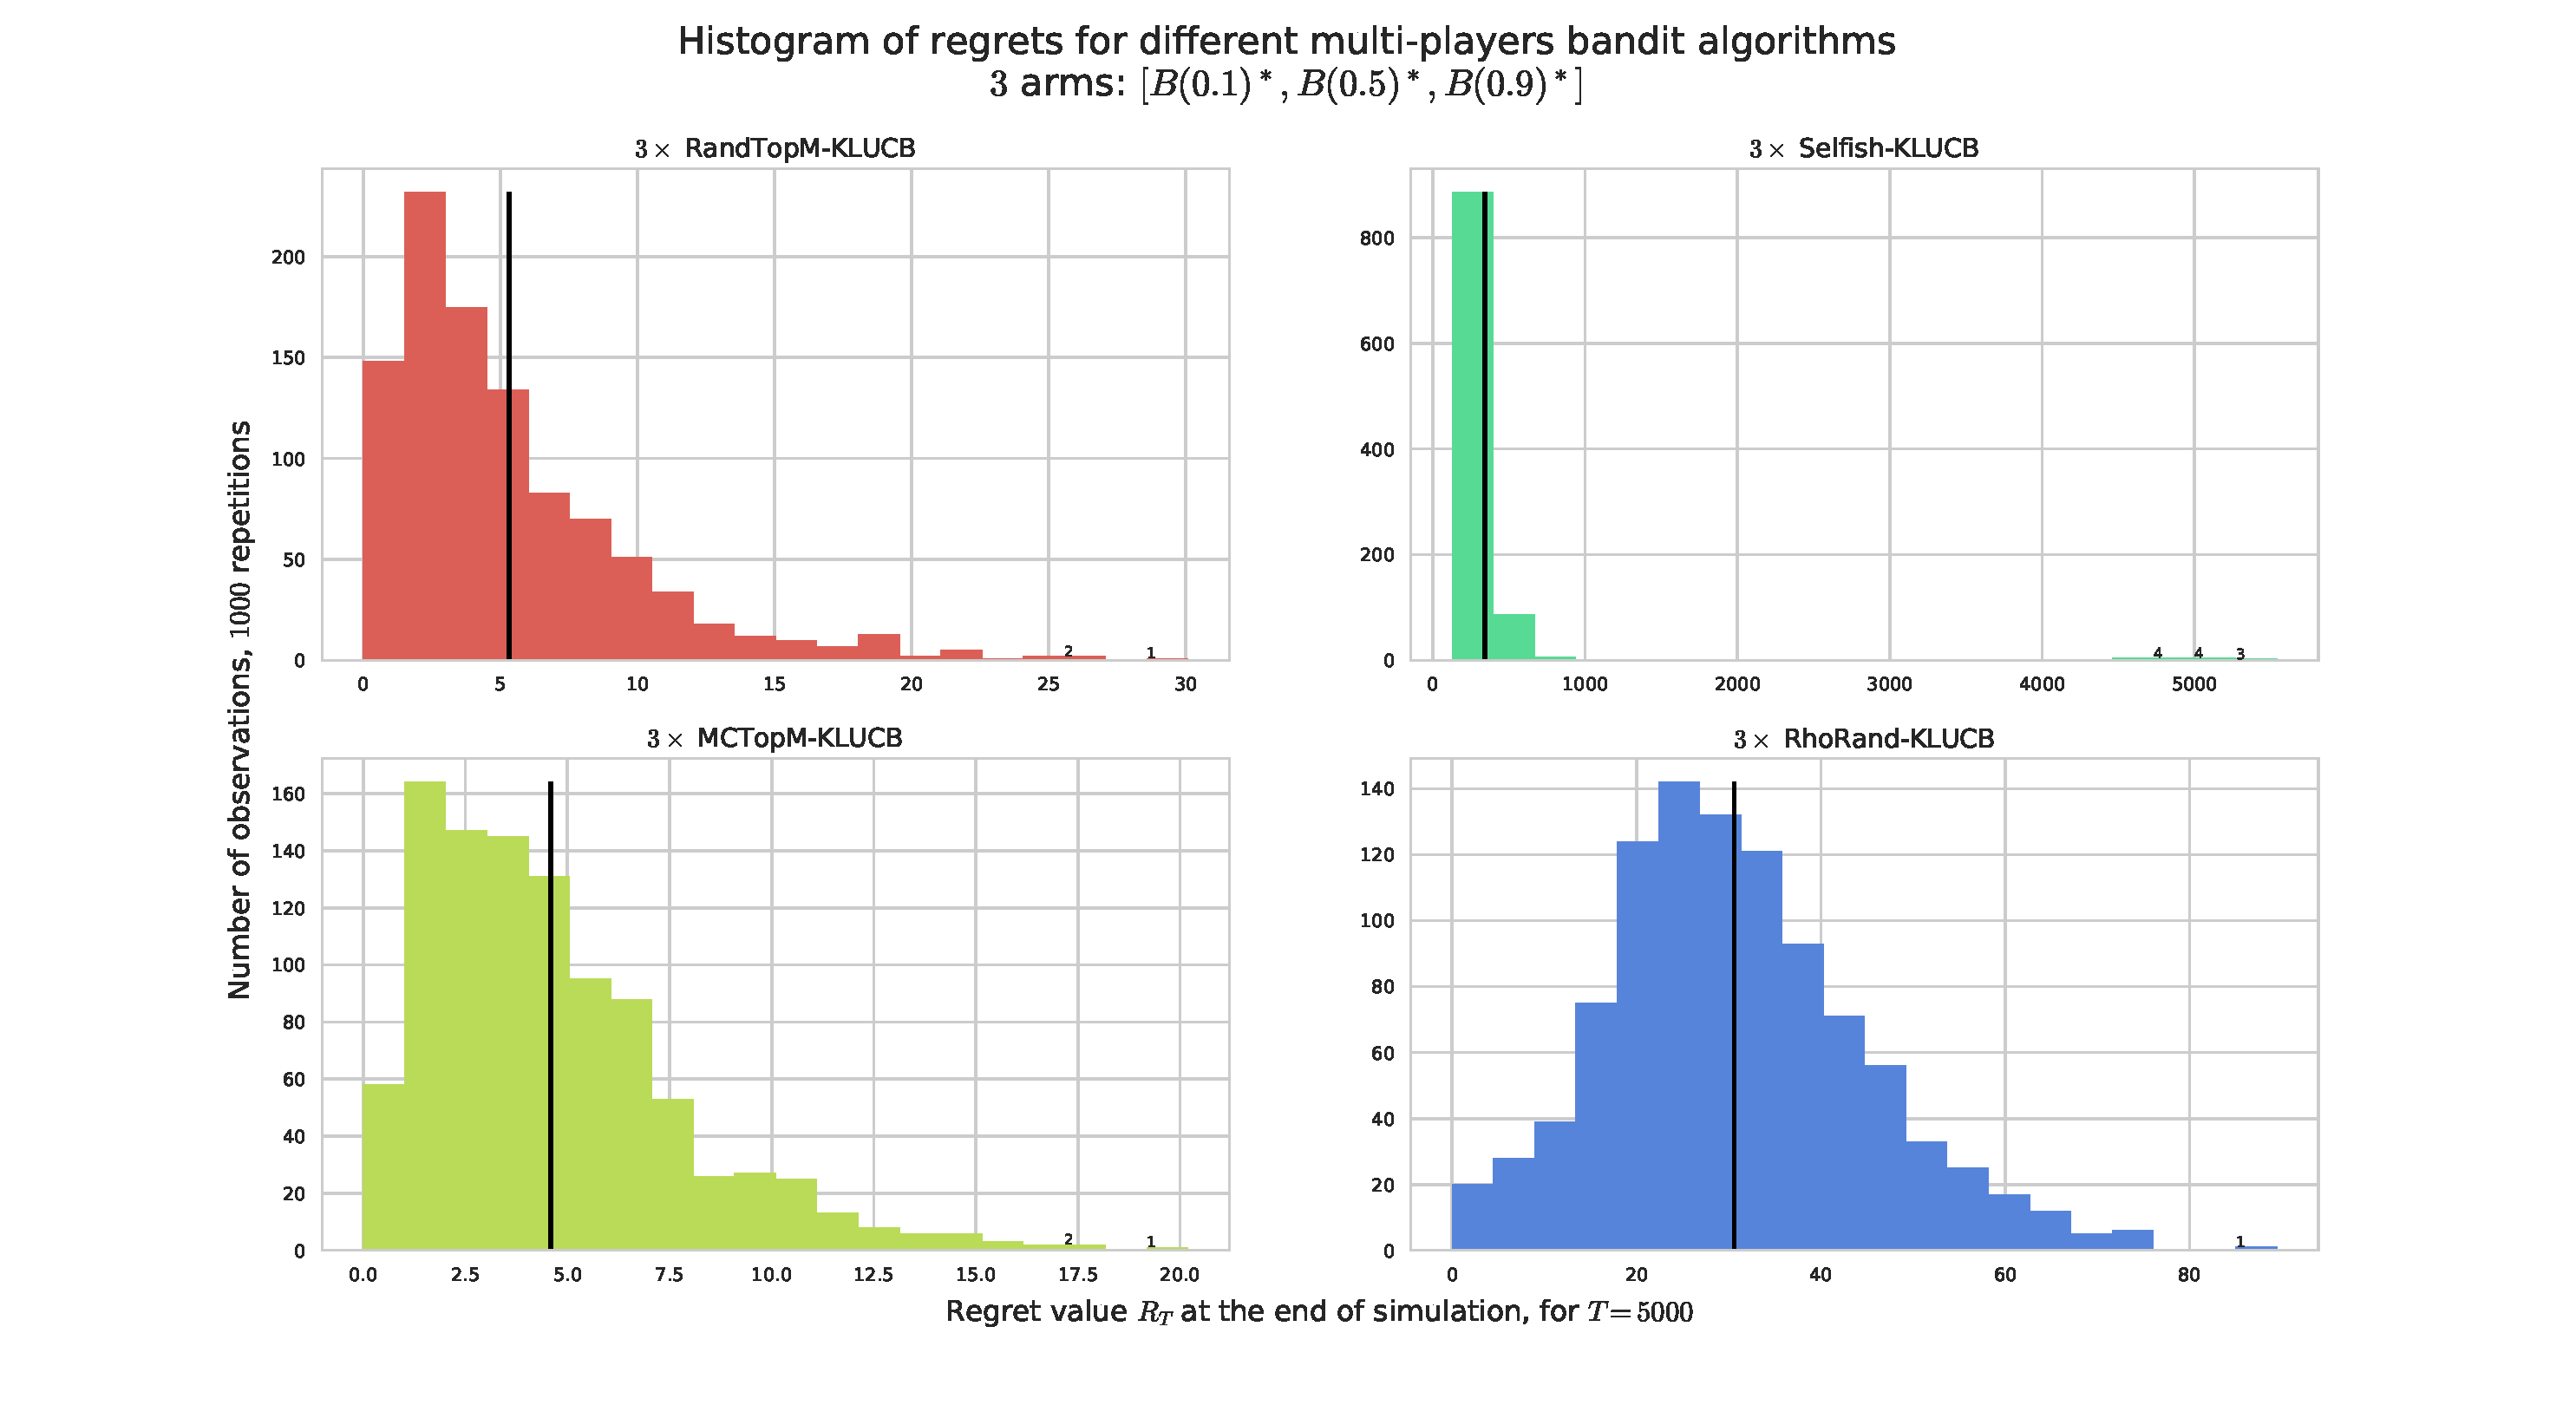
\includegraphics[width=1.10\textwidth]{MP__K3_M3_T5000_N1000__4_algos/all_HistogramsRegret____env1-1_1035303196230283176.pdf}
  % \end{subfigure}
  \caption[Failure case of \Selfish]{Regret for $M=2$ players, $K=3$ arms, horizon $T=5000$, $1000$ repetitions and $\boldsymbol{\mu} = [0.1, 0.5, 0.9]$. Axis $x$ is for regret (different scale for each part), and the \textcolor{darkgreen}{green} curve for \Selfish{} shows a small probability of having a linear regret ($17$ cases of $R_T \geq T$, out of $1000$). The regret for the three other algorithms is very small for this problem, always smaller than $100$ here.}
  \label{fig:5:selfish_fail1}
  % \vspace*{-15pt}  % XXX remove if problem
\end{figure}


%
% Regular plots of centralized regrets
%
\begin{figure}[!h]
  \centering
  % \begin{subfigure}[!h]{0.49\textwidth}
      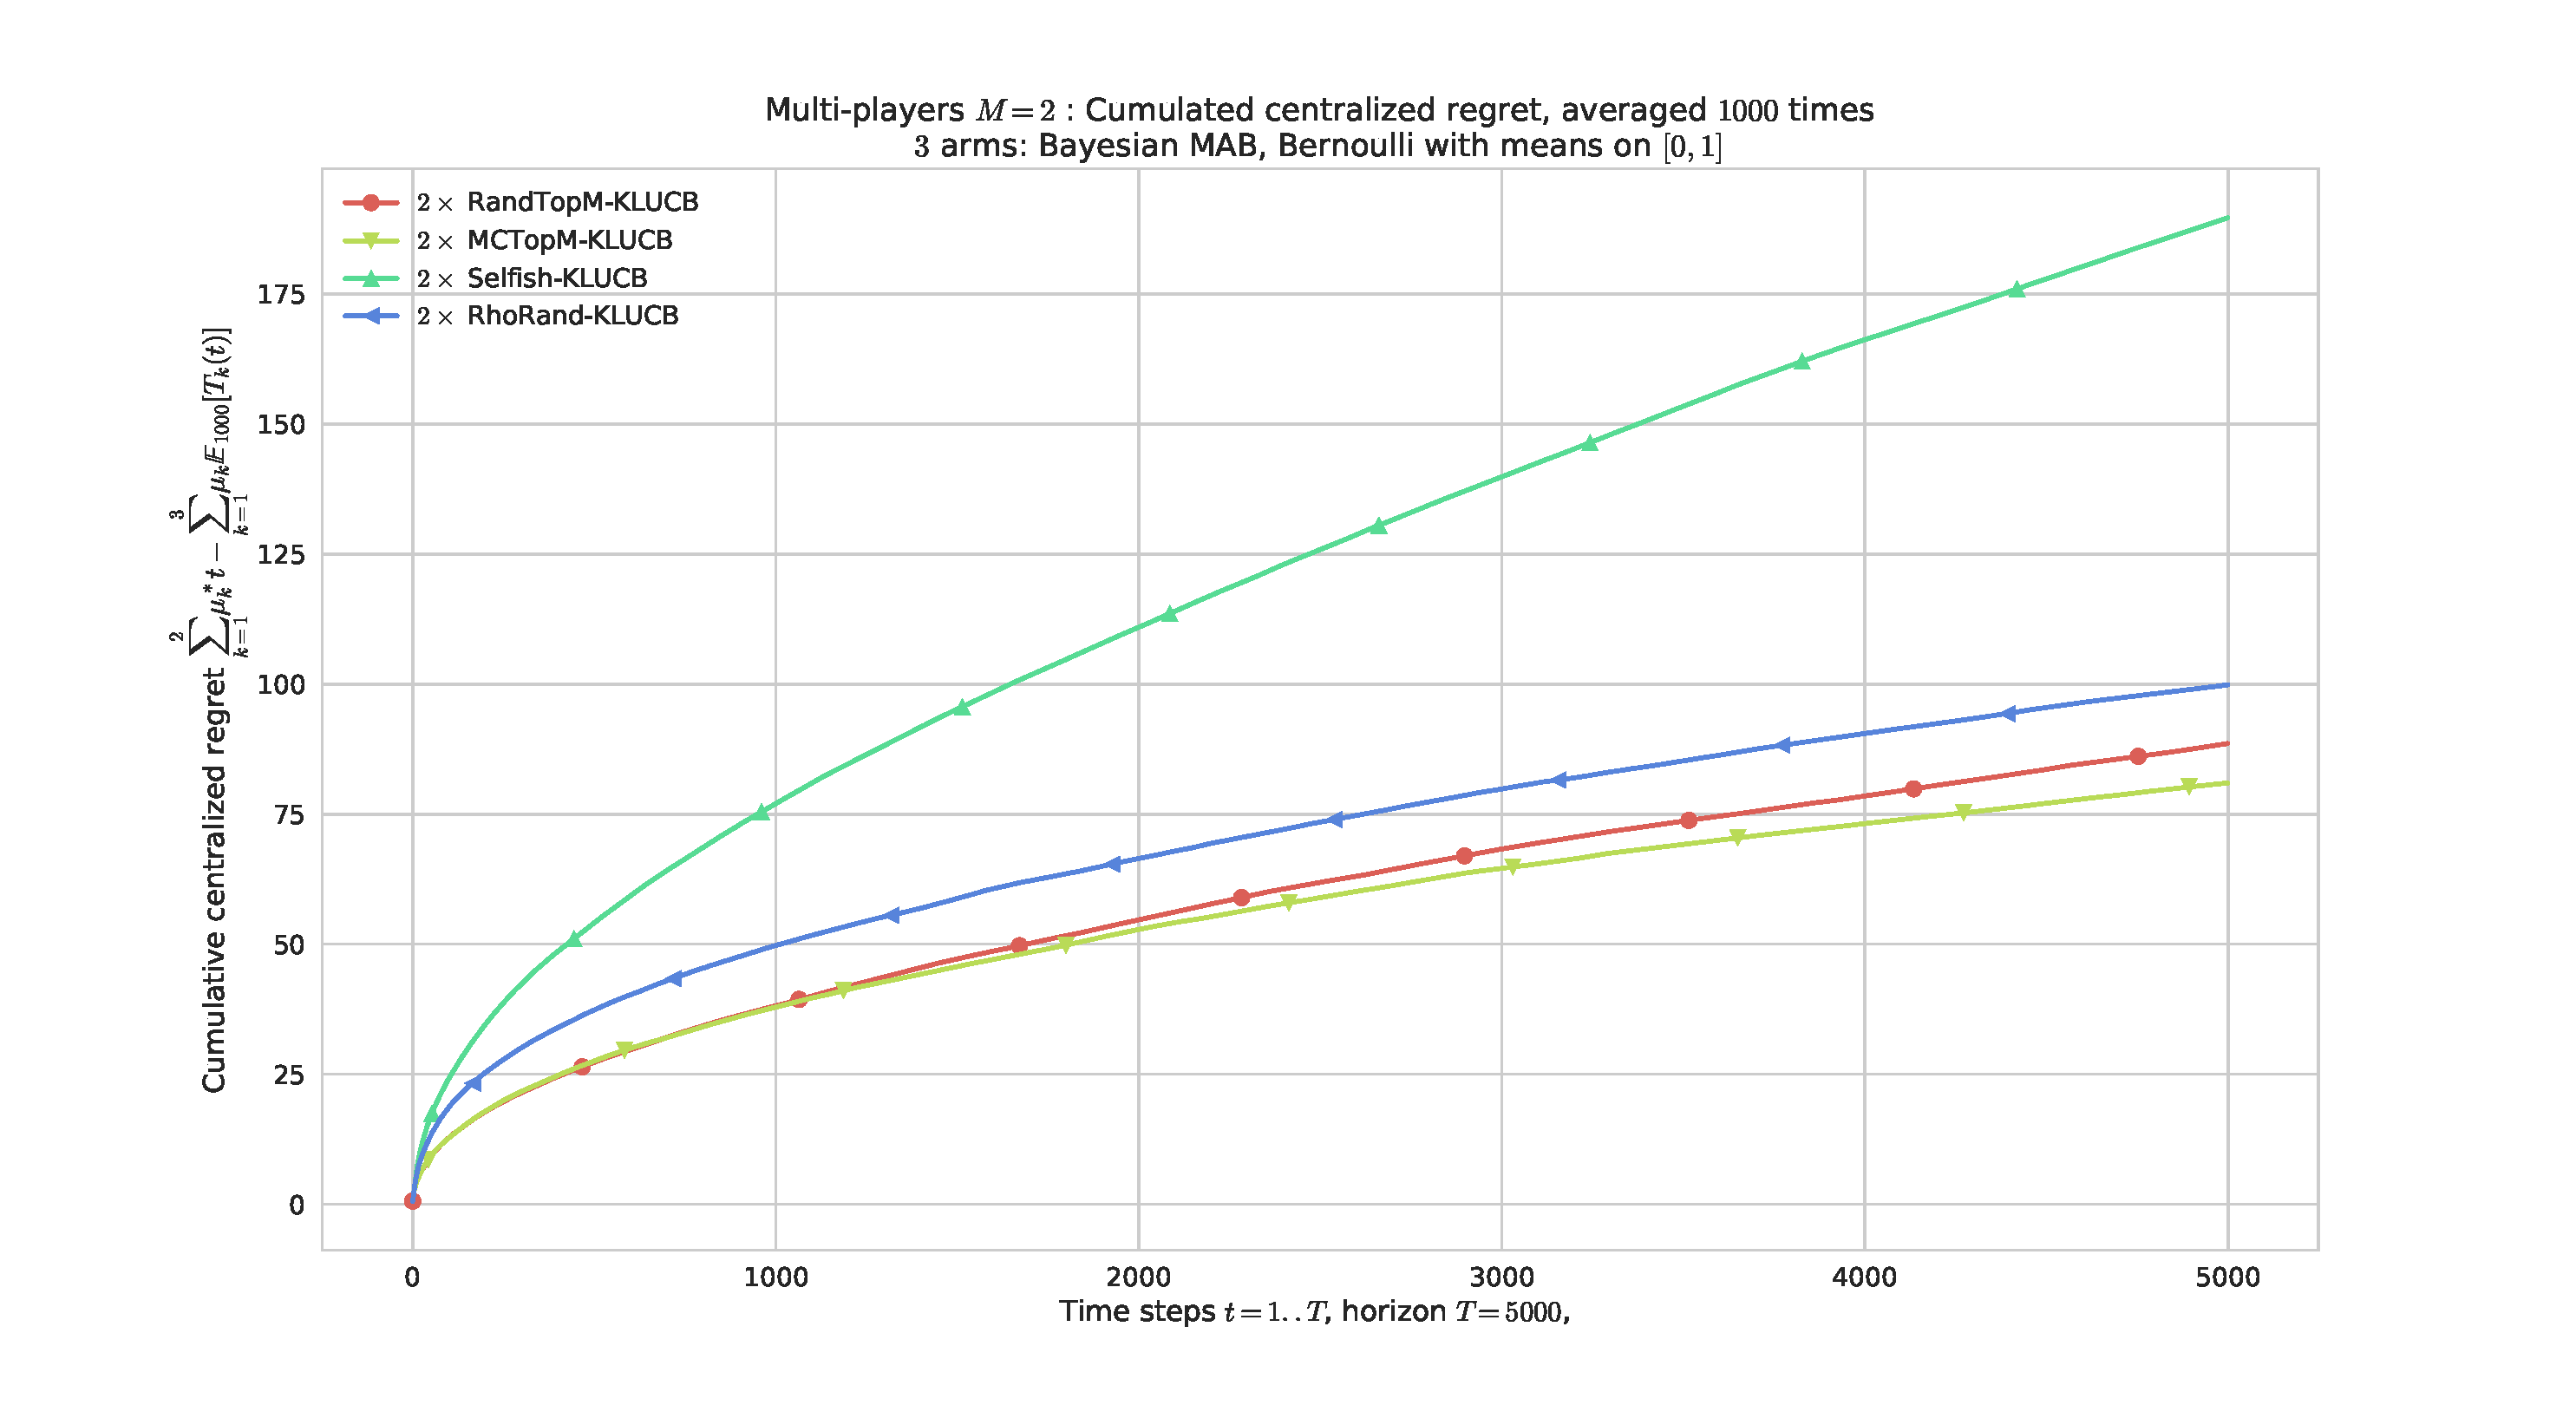
\includegraphics[width=1.05\textwidth]{MP__K3_M2_T5000_N1000__4_algos/all_RegretCentralized____env1-1_2643560344649862285.pdf}
  % \end{subfigure}
  % ~
  % \begin{subfigure}[!h]{0.49\textwidth}
      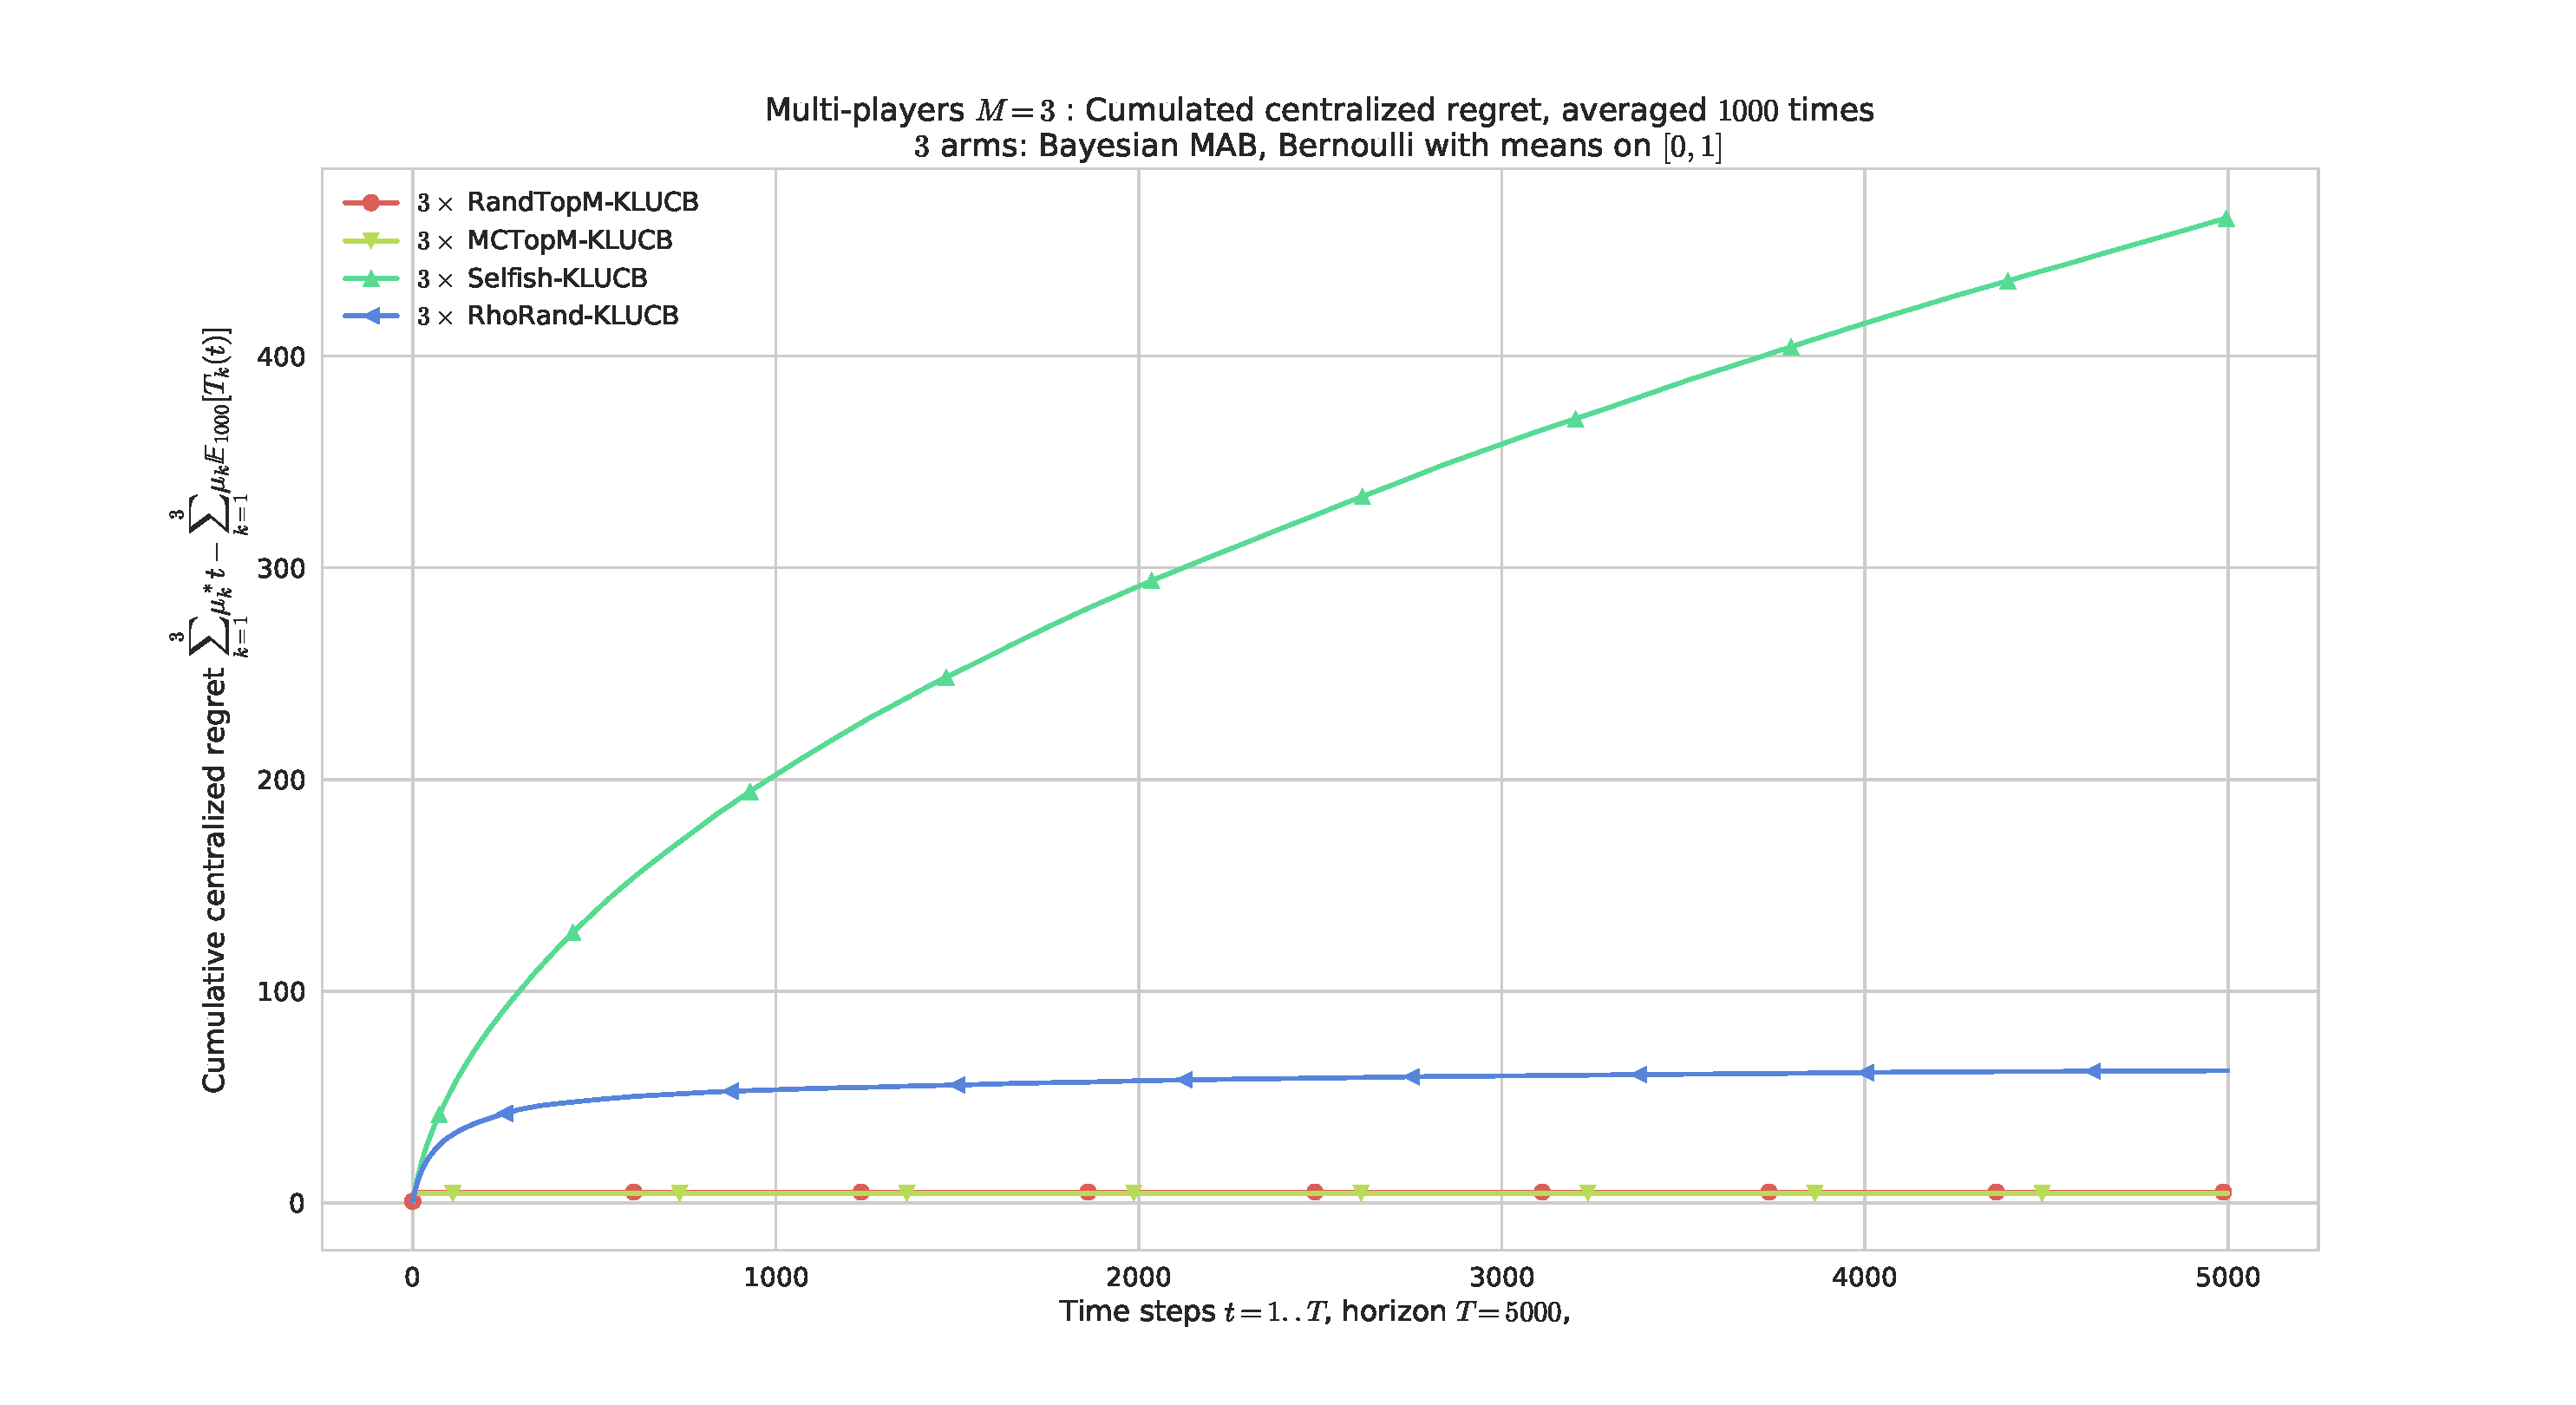
\includegraphics[width=1.05\textwidth]{MP__K3_M3_T5000_N1000__4_algos/all_RegretCentralized____env1-1_4683123079851881812.pdf}
  % \end{subfigure}
  \caption[Second failure case of \Selfish]{Regret, $M=2$ and $M=3$ players, $K=3$ arms, horizon $T=5000$, against $1000$ problems $\boldsymbol{\mu}$ uniformly sampled in $[0,1]^K$. \Selfish{} (top curve in \textcolor{darkgreen}{green}) clearly fails in such setting with small $K$.}
  \label{fig:5:selfish_fail2}
  % \vspace*{-15pt}  % XXX remove if problem
\end{figure}

%
% Regular plots of centralized regrets
%
\begin{figure}[!h]
  \centering
  % \begin{subfigure}[!h]{1.00\textwidth}
      % 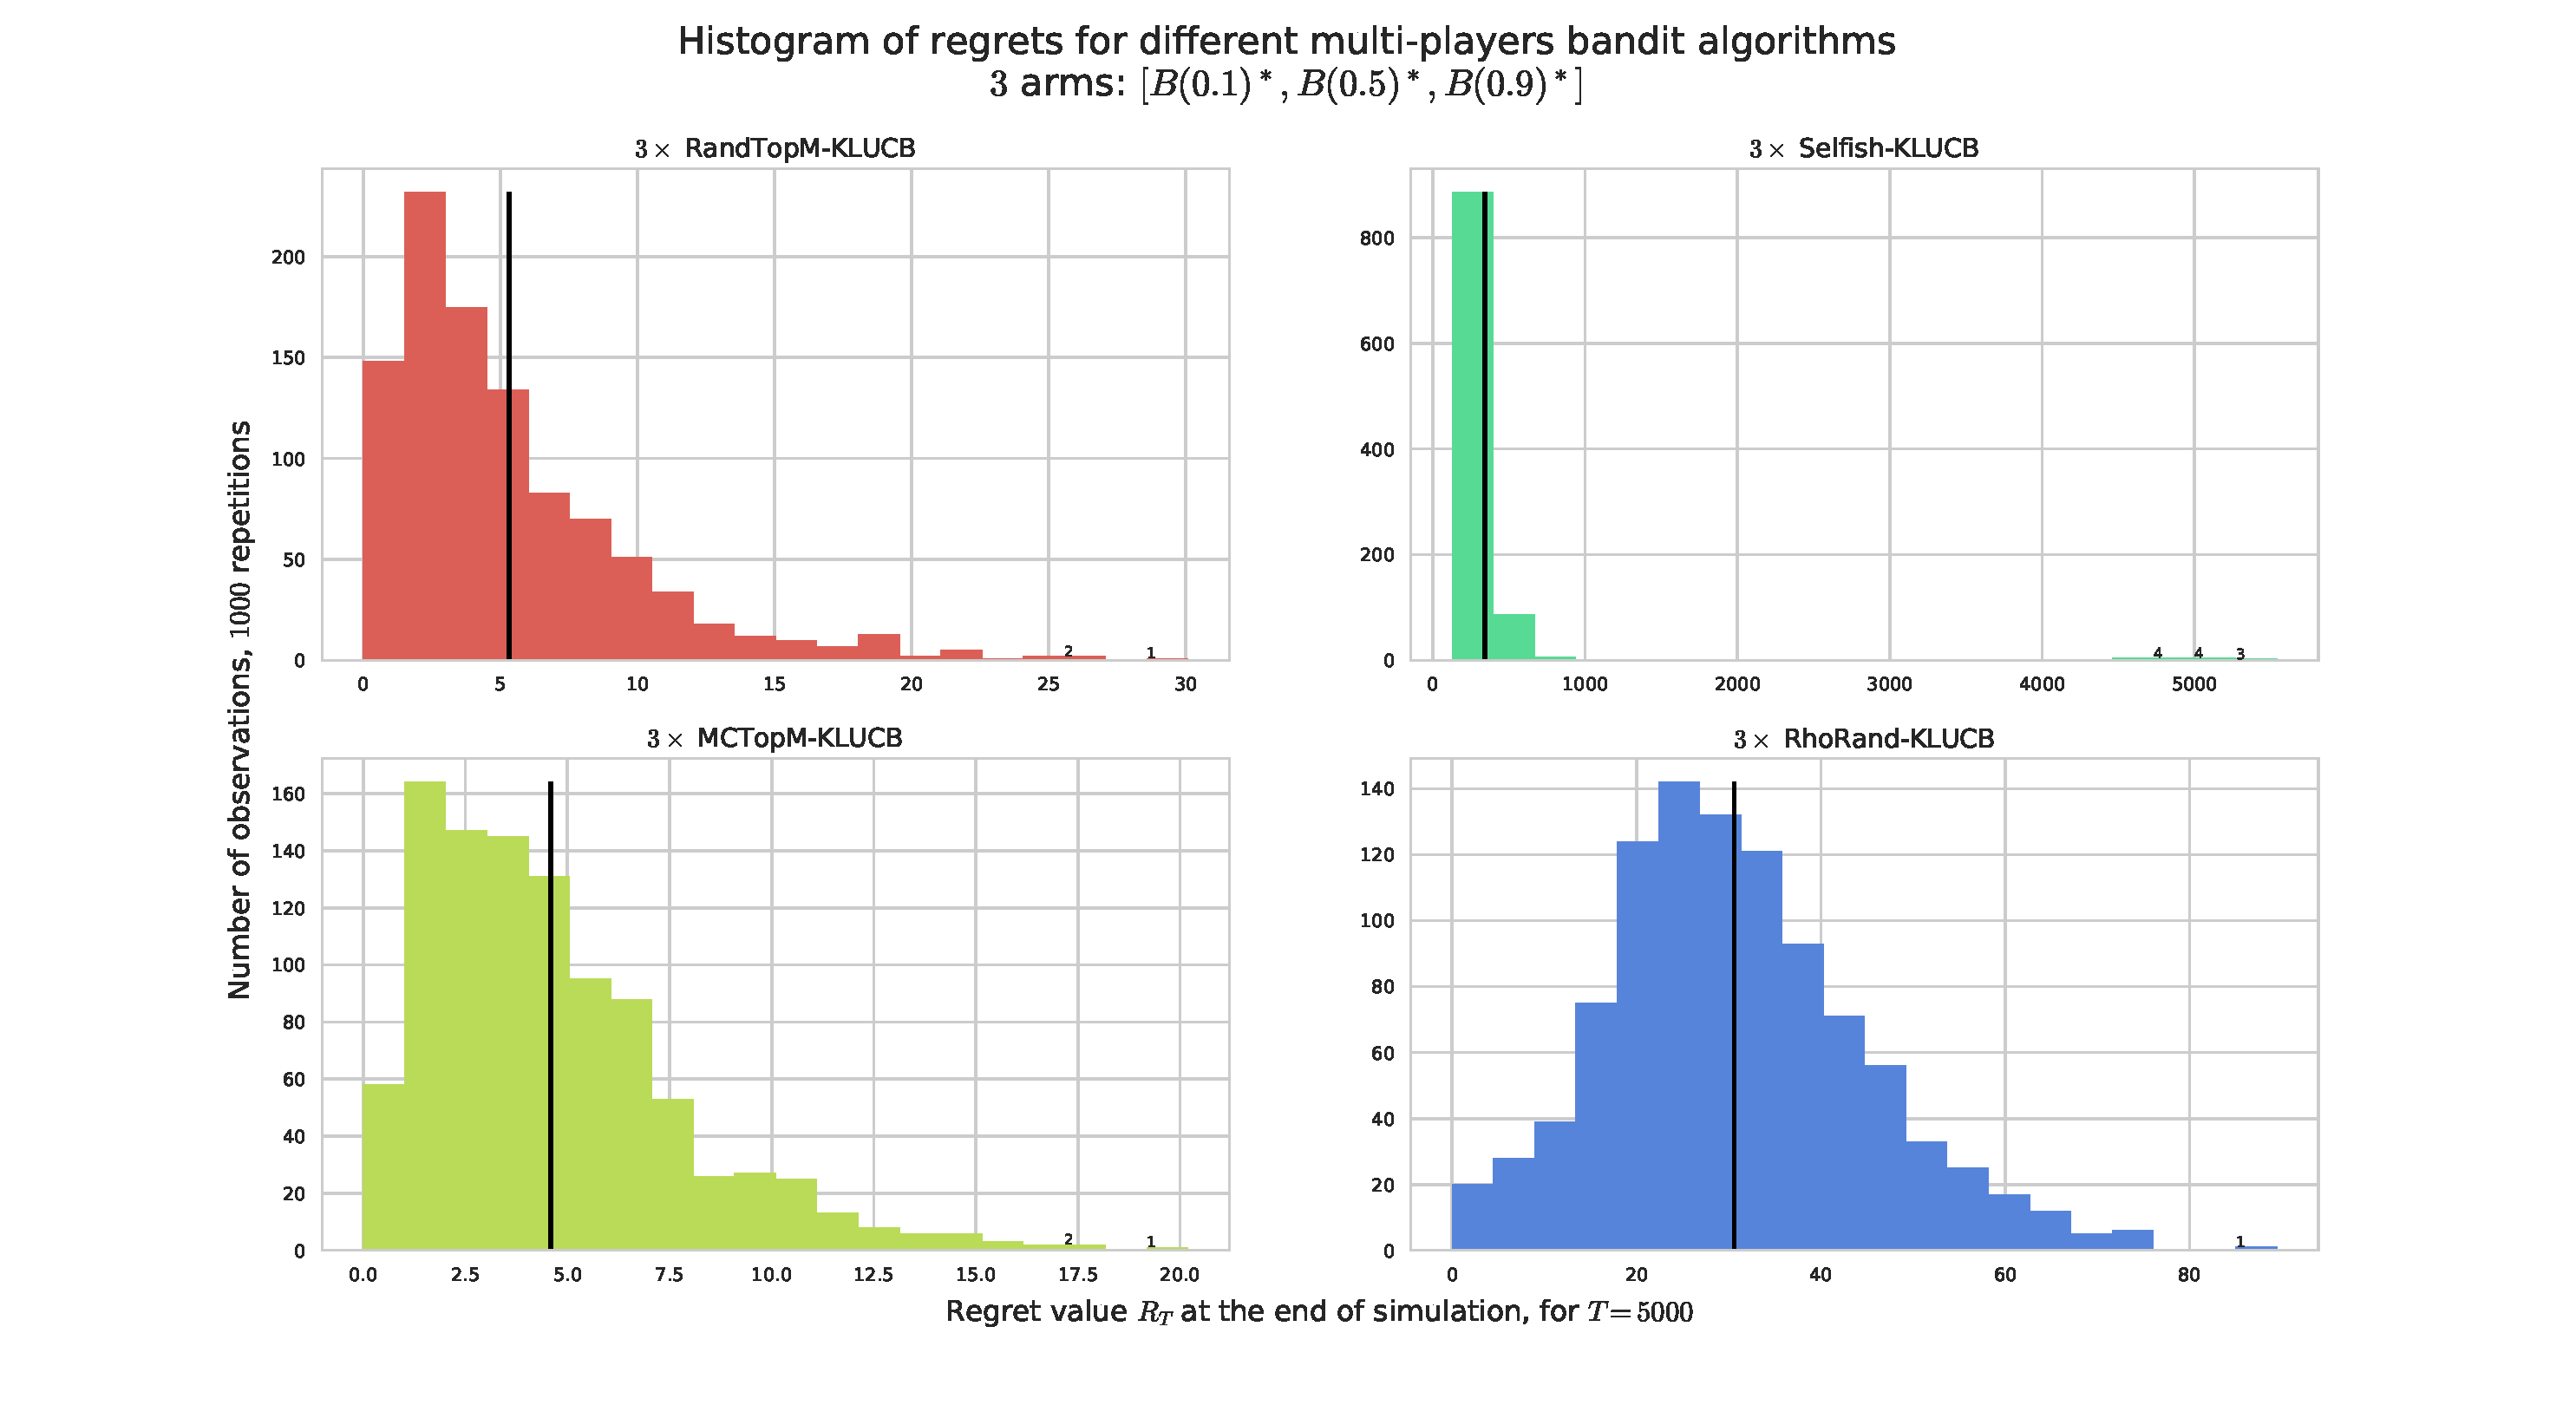
\includegraphics[width=1.00\textwidth]{MP__K3_M3_T5000_N1000__4_algos/all_HistogramsRegret____env1-1_1035303196230283176.pdf}
      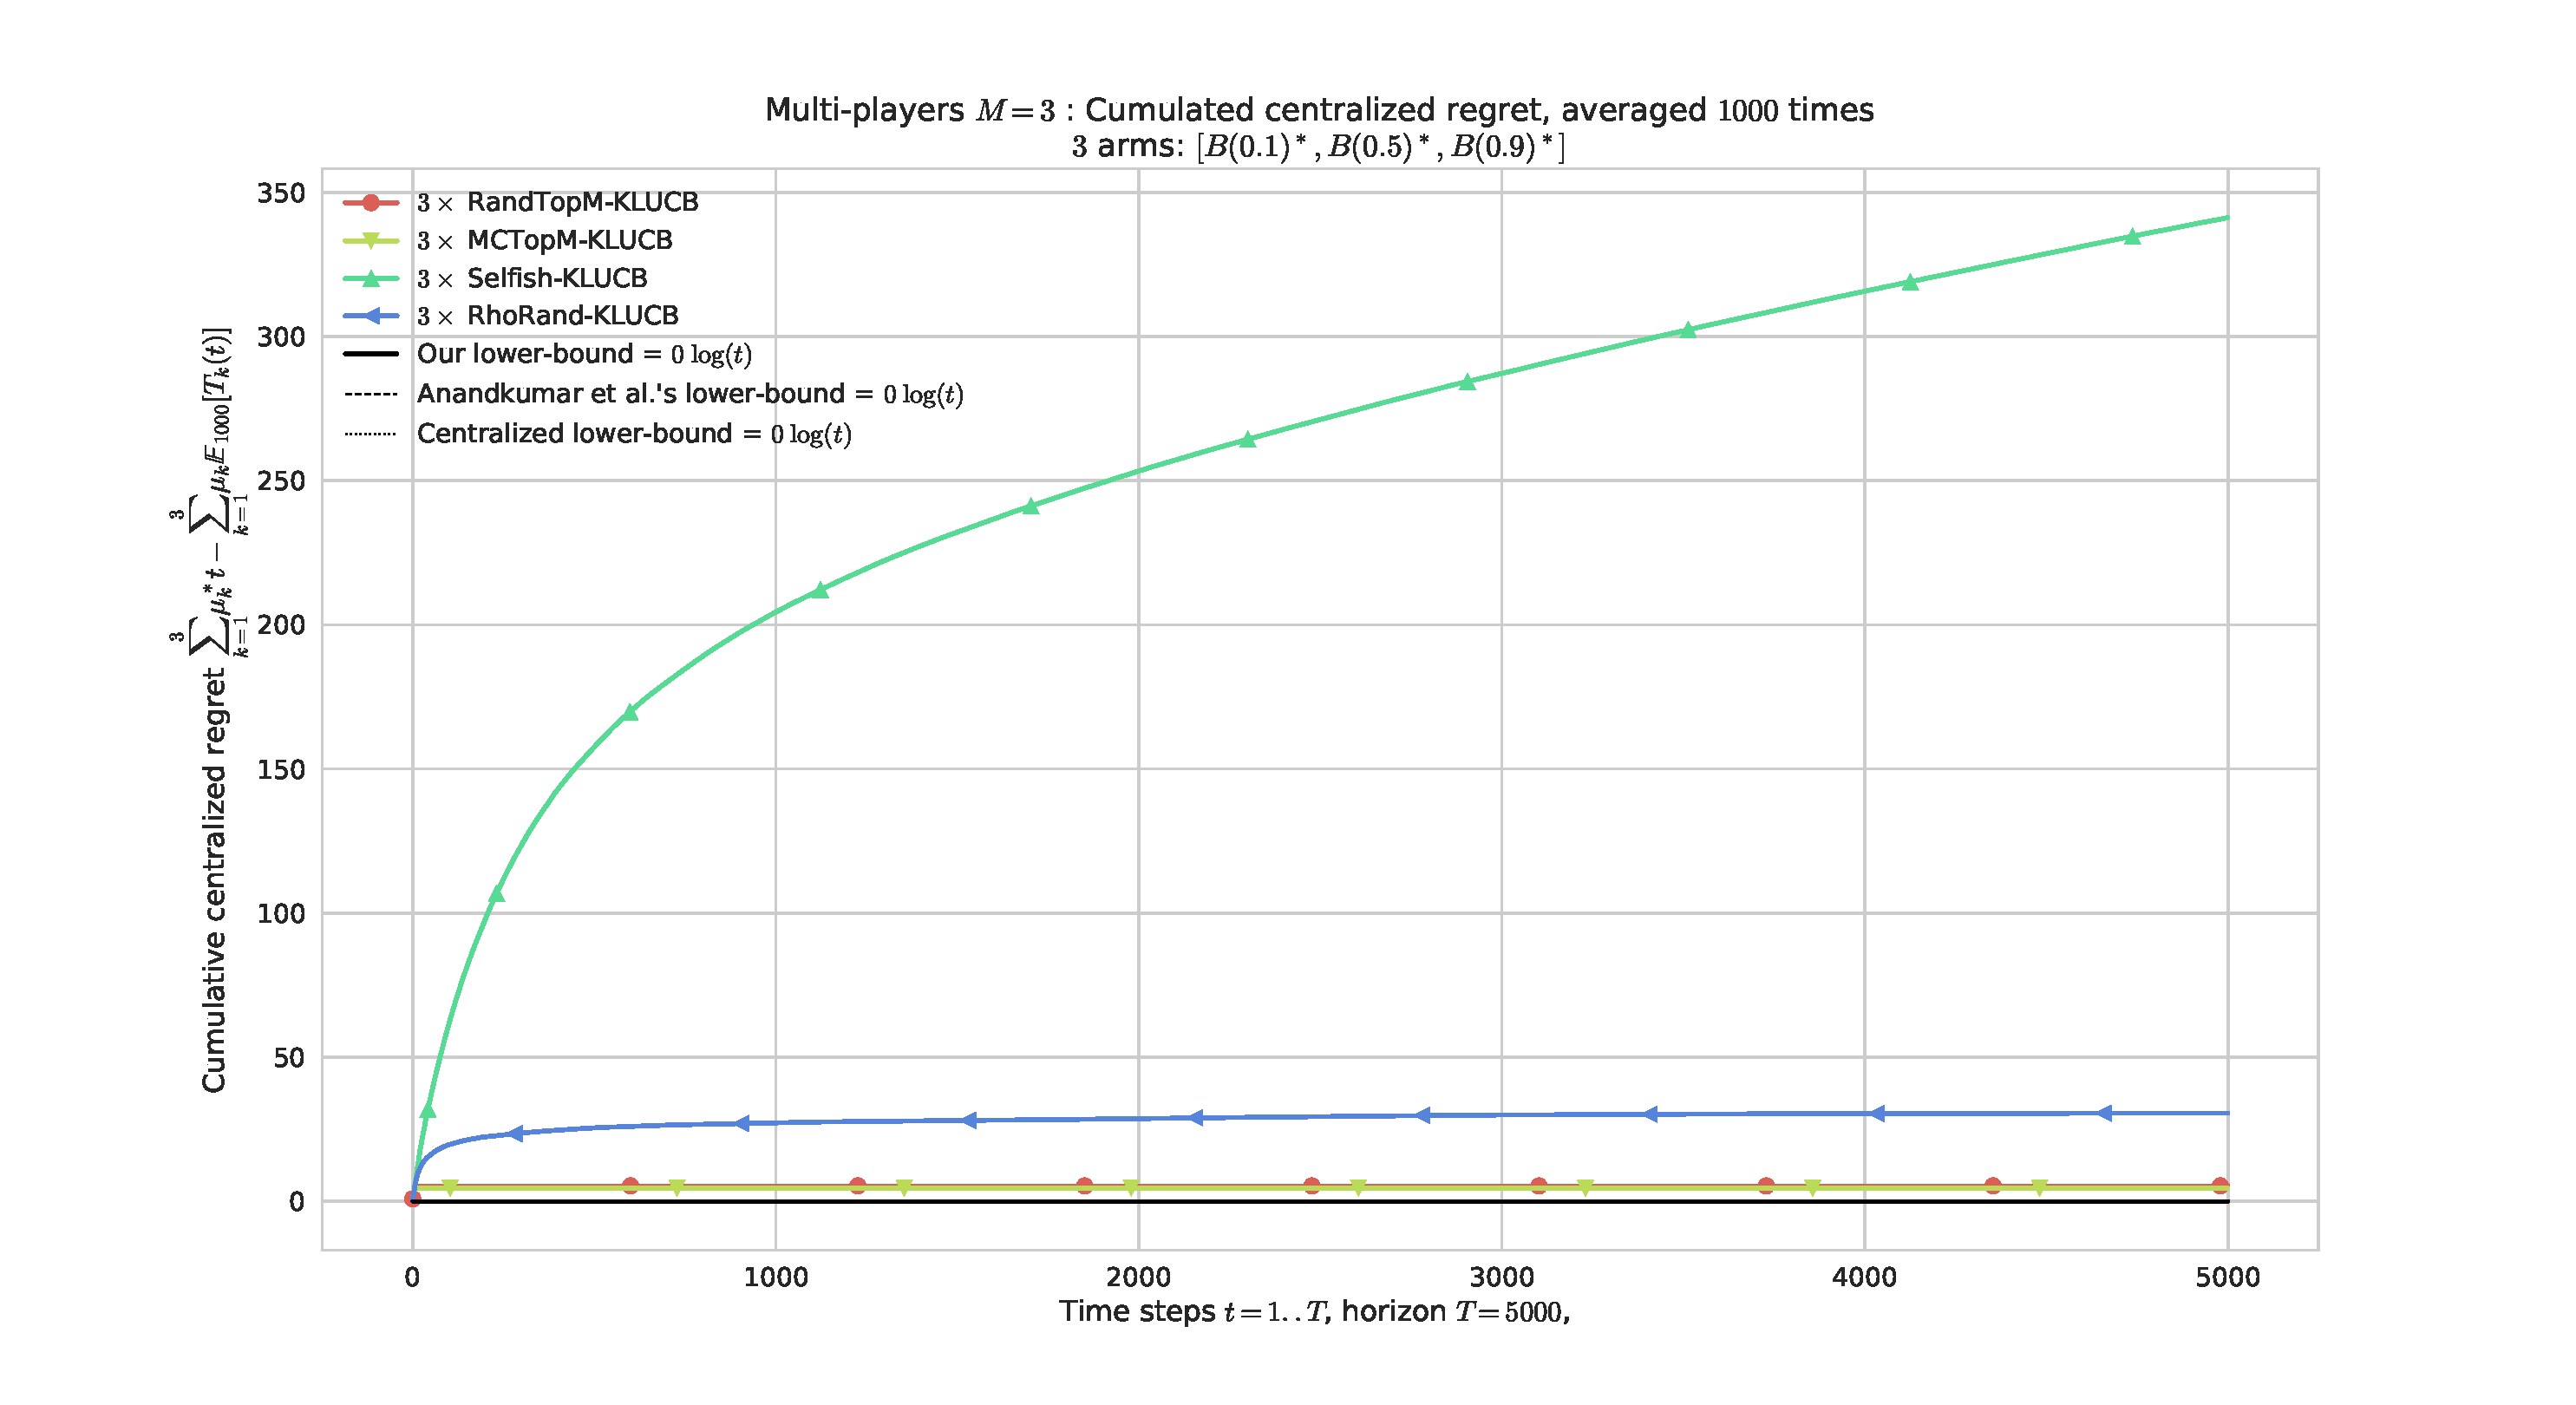
\includegraphics[width=1.00\textwidth]{MP__K3_M3_T5000_N1000__4_algos/all_RegretCentralized____env1-1_1035303196230283176.pdf}
      % 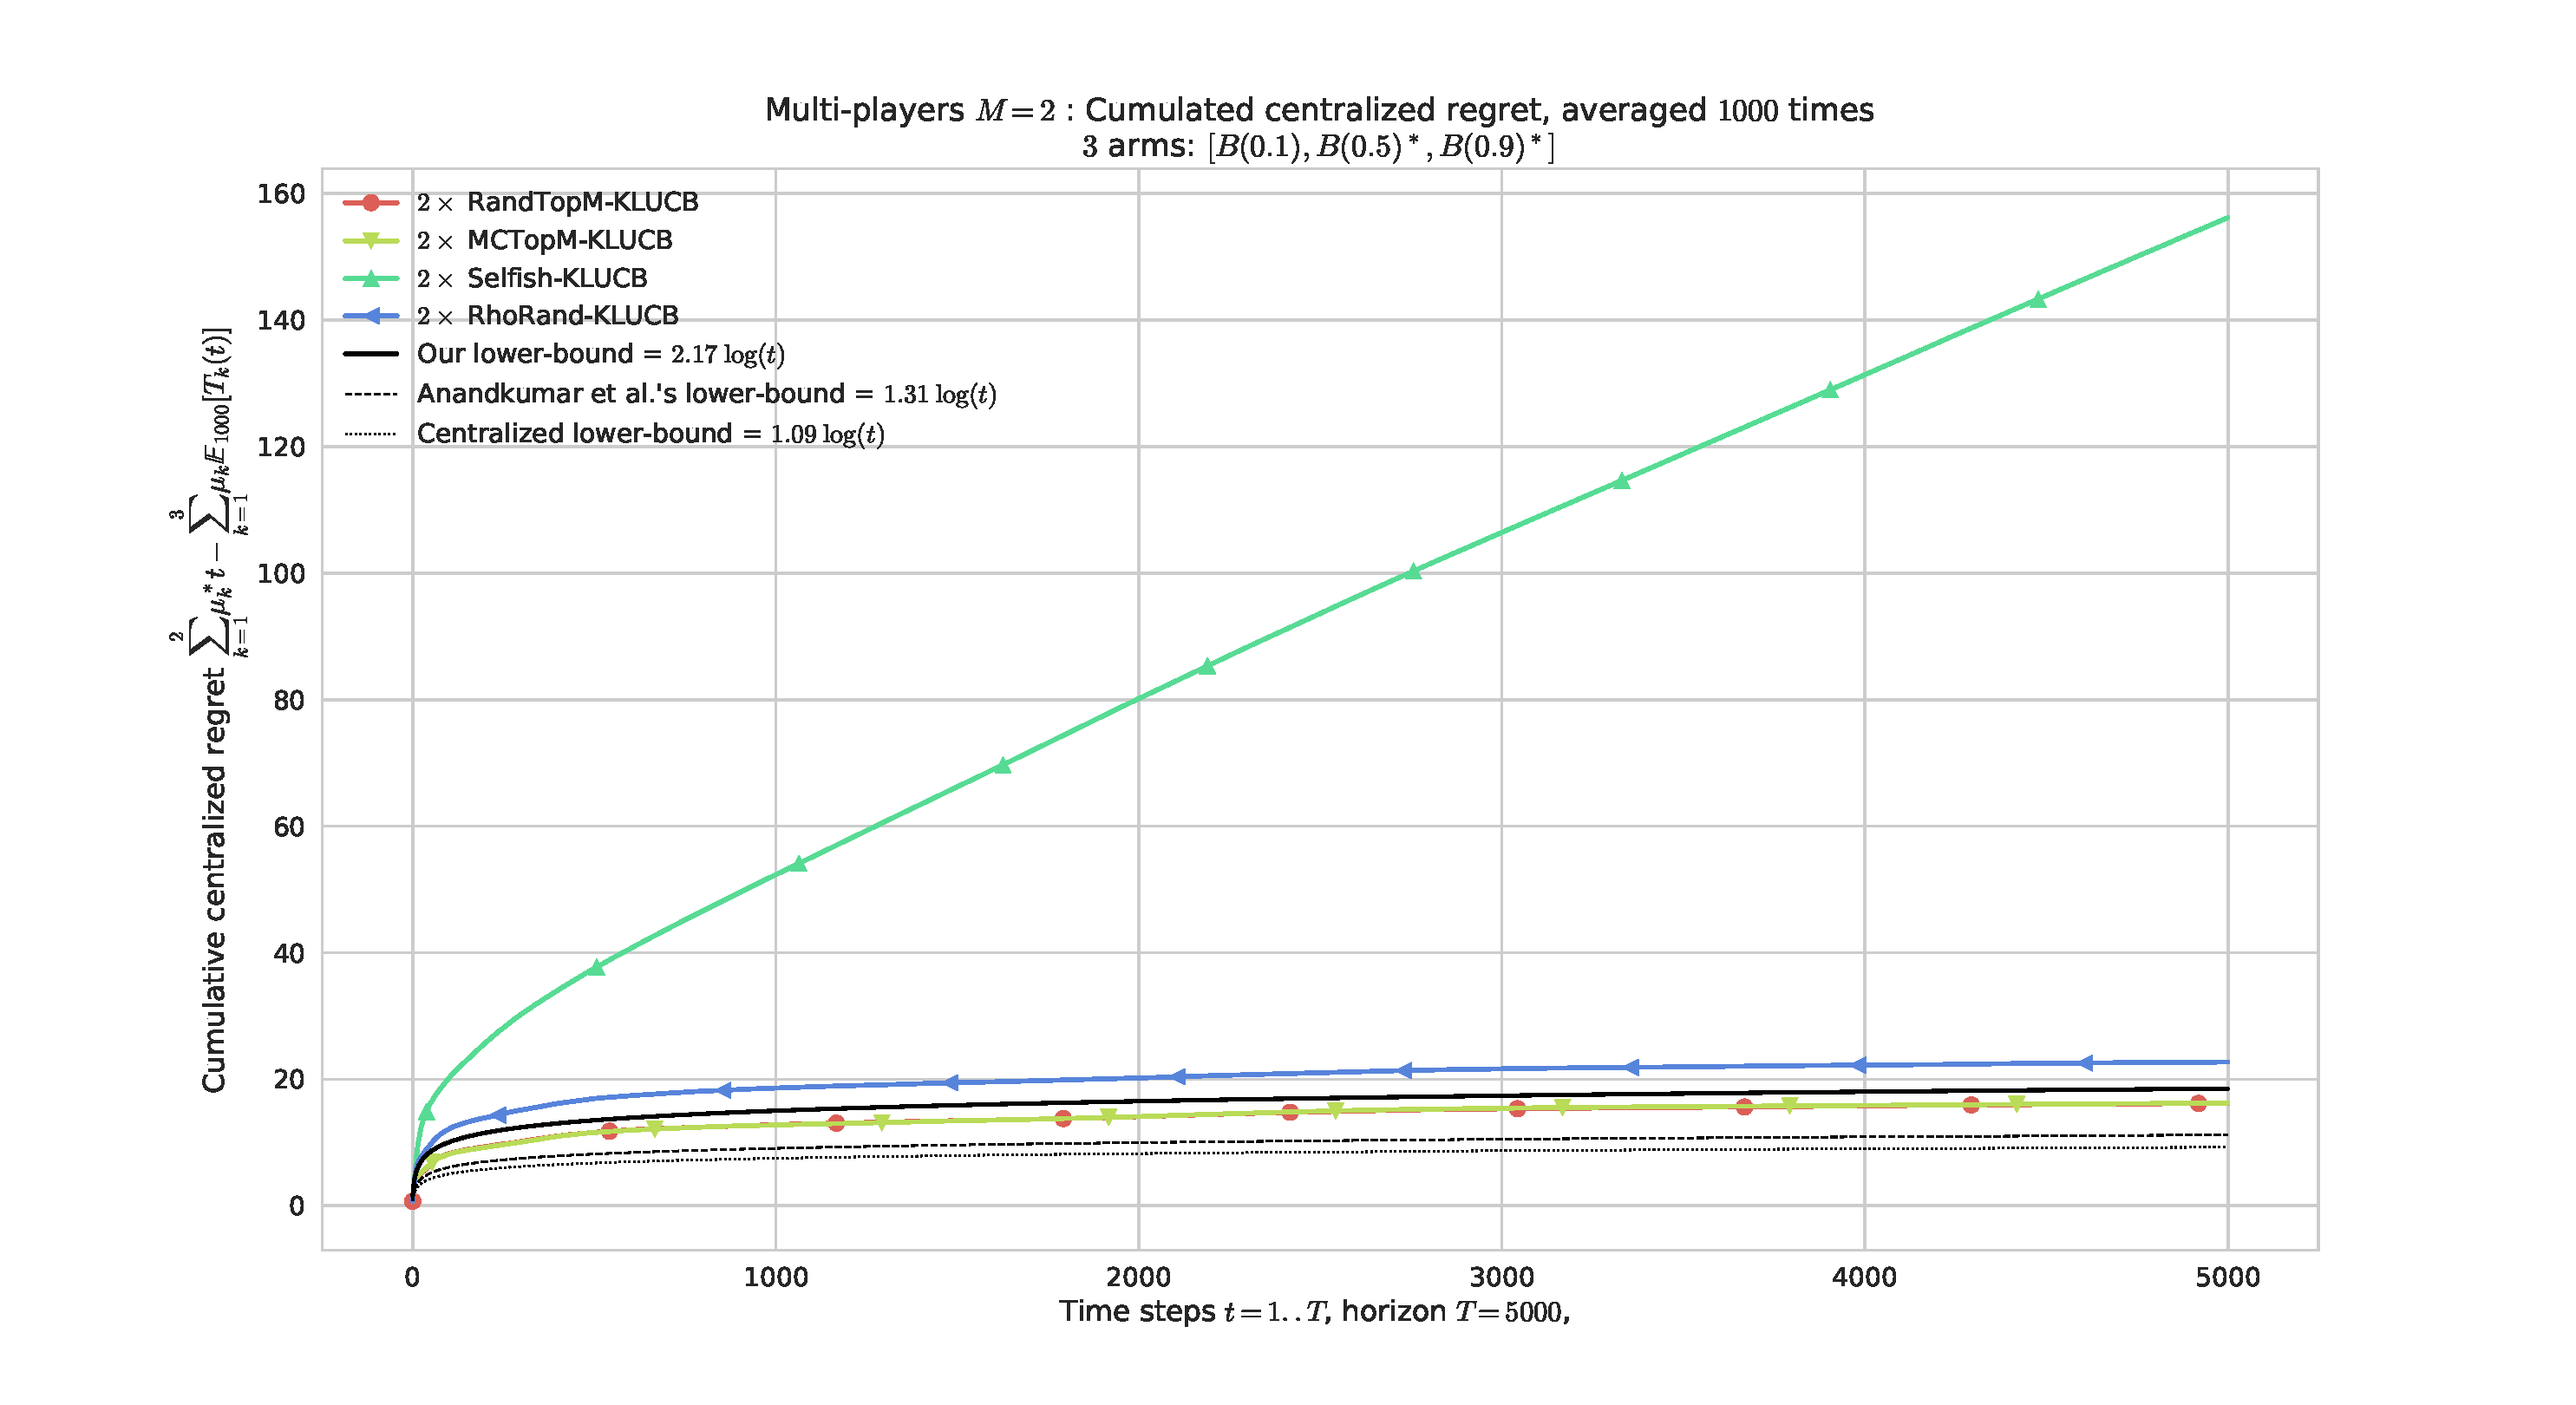
\includegraphics[width=1.00\textwidth]{MP__K3_M2_T5000_N1000__4_algos/all_RegretCentralized____env1-1_5016720151160452442.pdf}
  % \end{subfigure}
  ~
  % \begin{subfigure}[!h]{1.00\textwidth}
      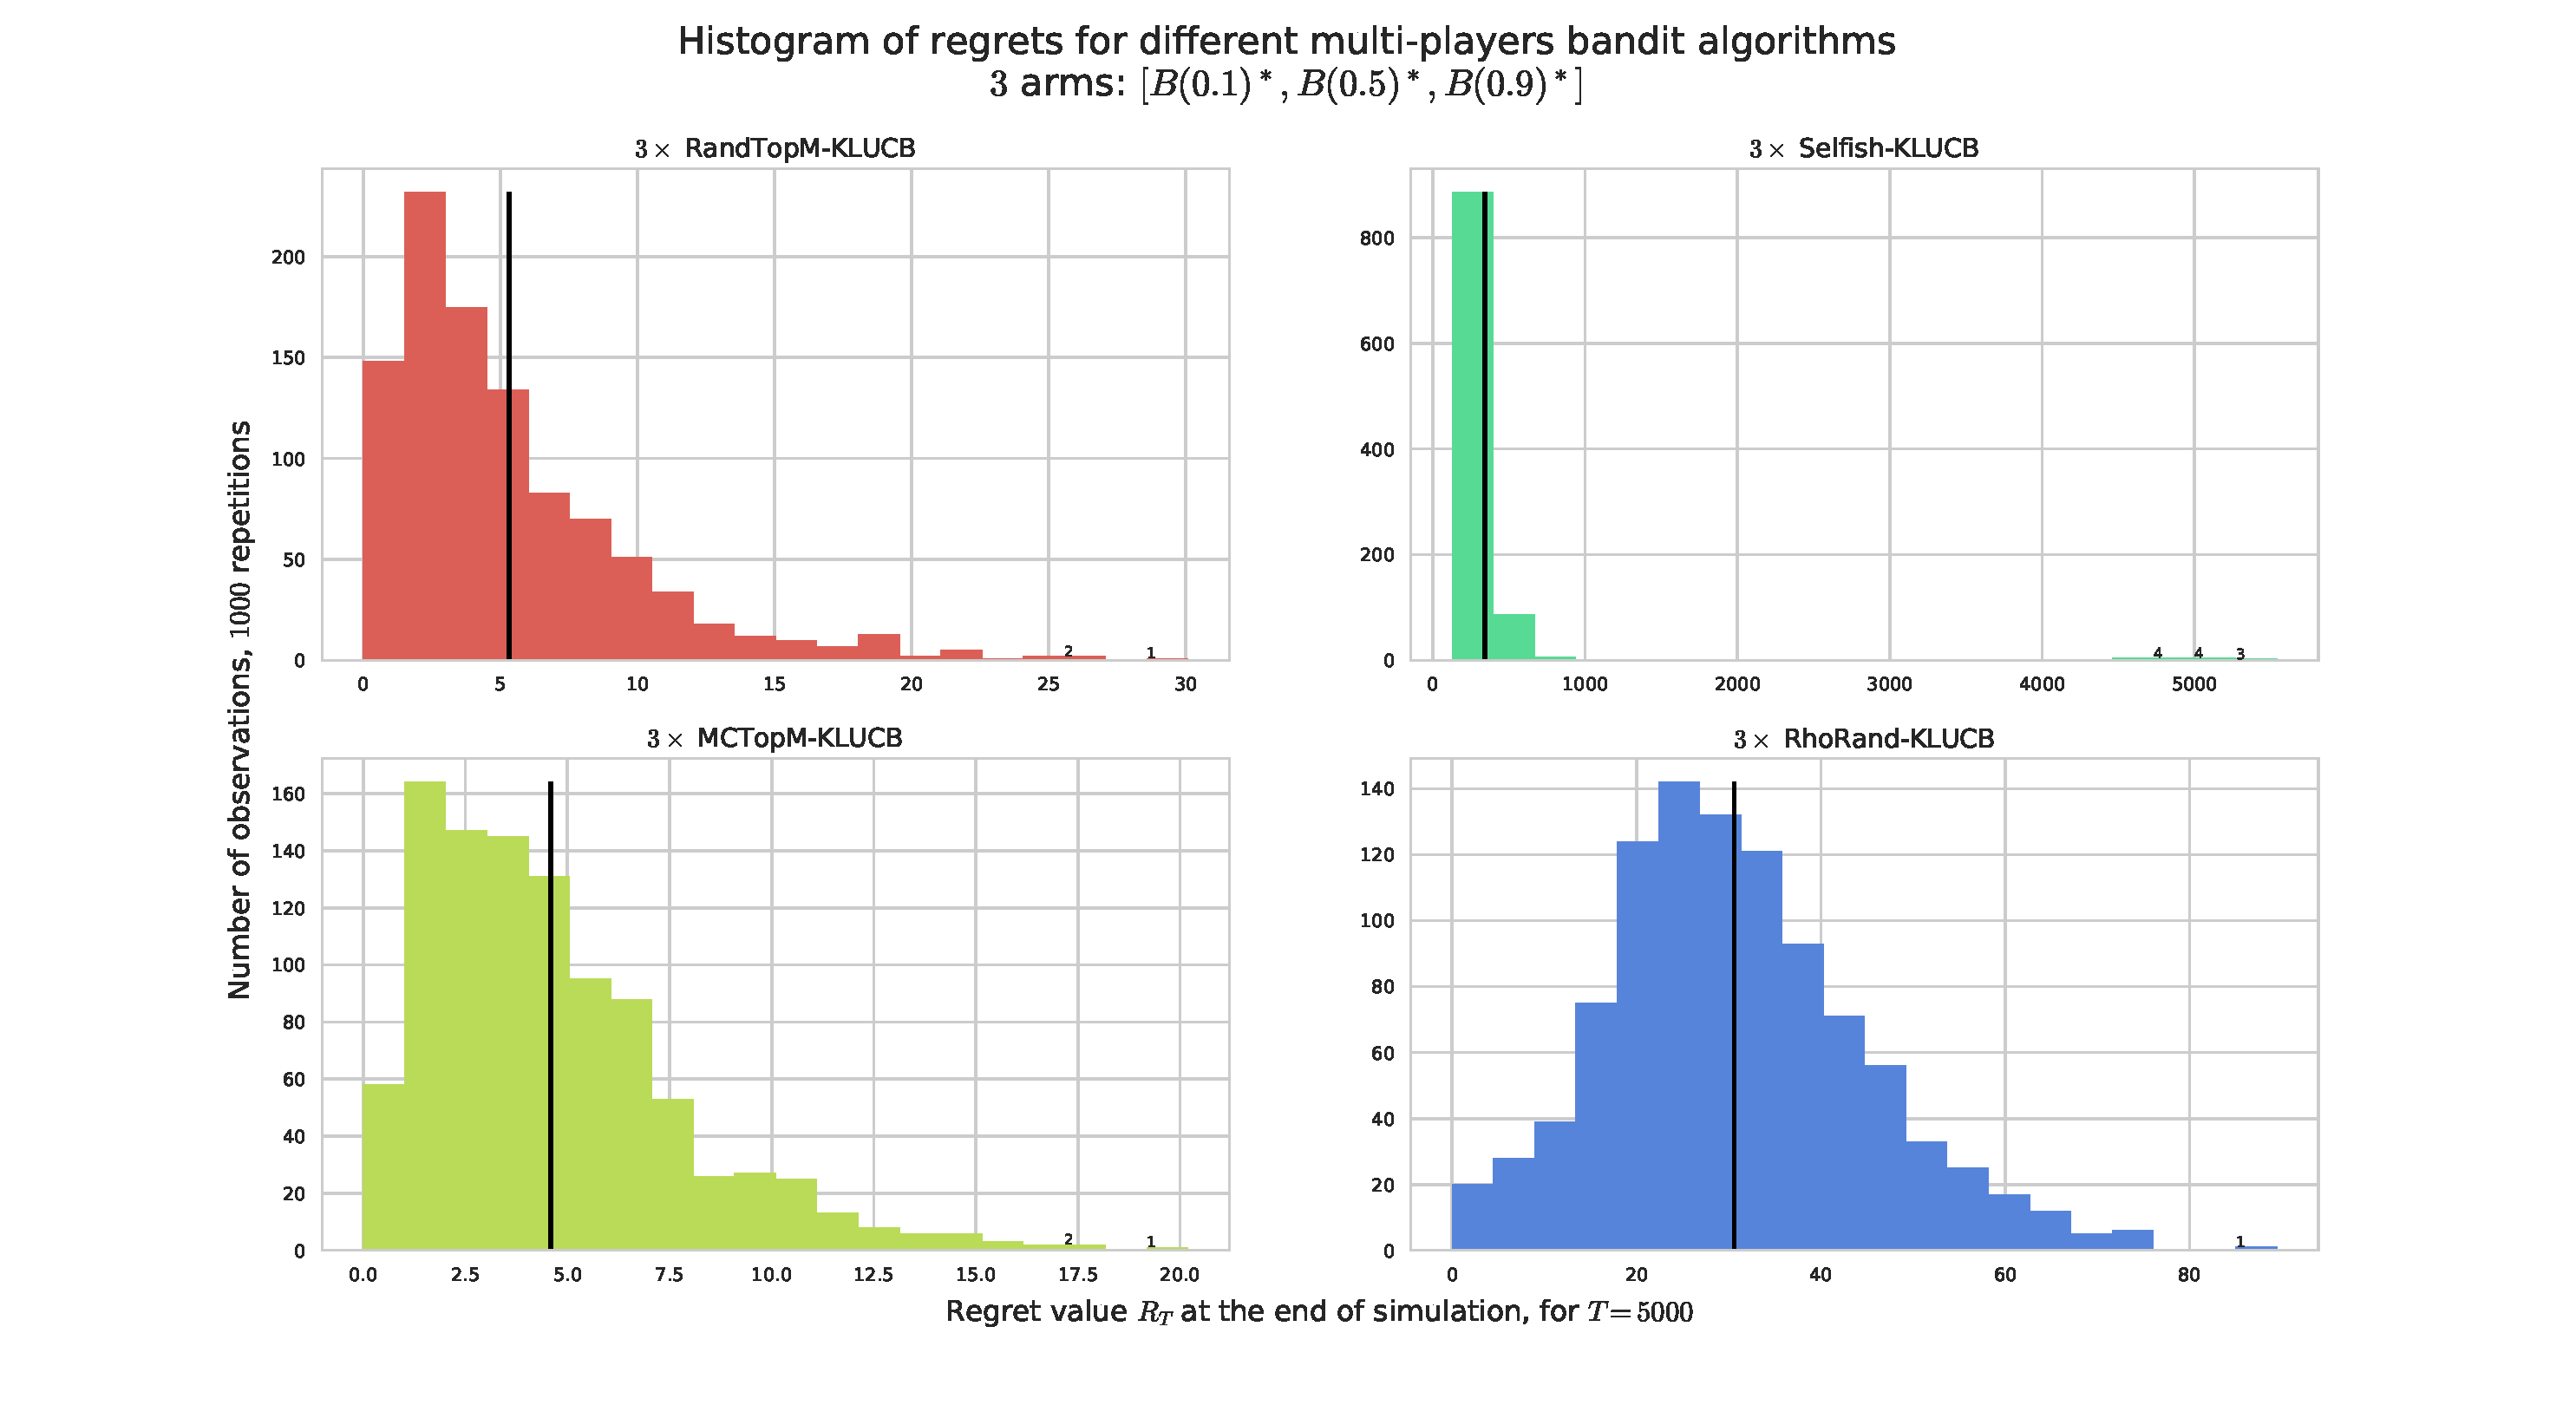
\includegraphics[width=1.00\textwidth]{MP__K3_M3_T5000_N1000__4_algos/all_HistogramsRegret____env1-1_1035303196230283176.pdf}
  % \end{subfigure}
  \caption[Third failure case of \Selfish]{Regret for $M=3$ players, $K=3$ arms, horizon $T=5000$, $1000$ repetitions and $\boldsymbol{\mu} = [0.1, 0.5, 0.9]$. Axis $x$ is for regret (different scale for each), and the top \textcolor{darkgreen}{green} curve for \Selfish{} shows a small probability of having a linear regret ($11$ cases of $R_T \geq T$, out of $1000$). The regret for the three other algorithms is very small for this problem, and even appears constant.}
  \label{fig:5:selfish_fail3}
  % \vspace*{-15pt}  % XXX remove if problem
\end{figure}

%
% Regular plots of centralized regrets
%

\begin{figure}[!h]
  \centering
  % \begin{subfigure}[!h]{1.00\textwidth}
      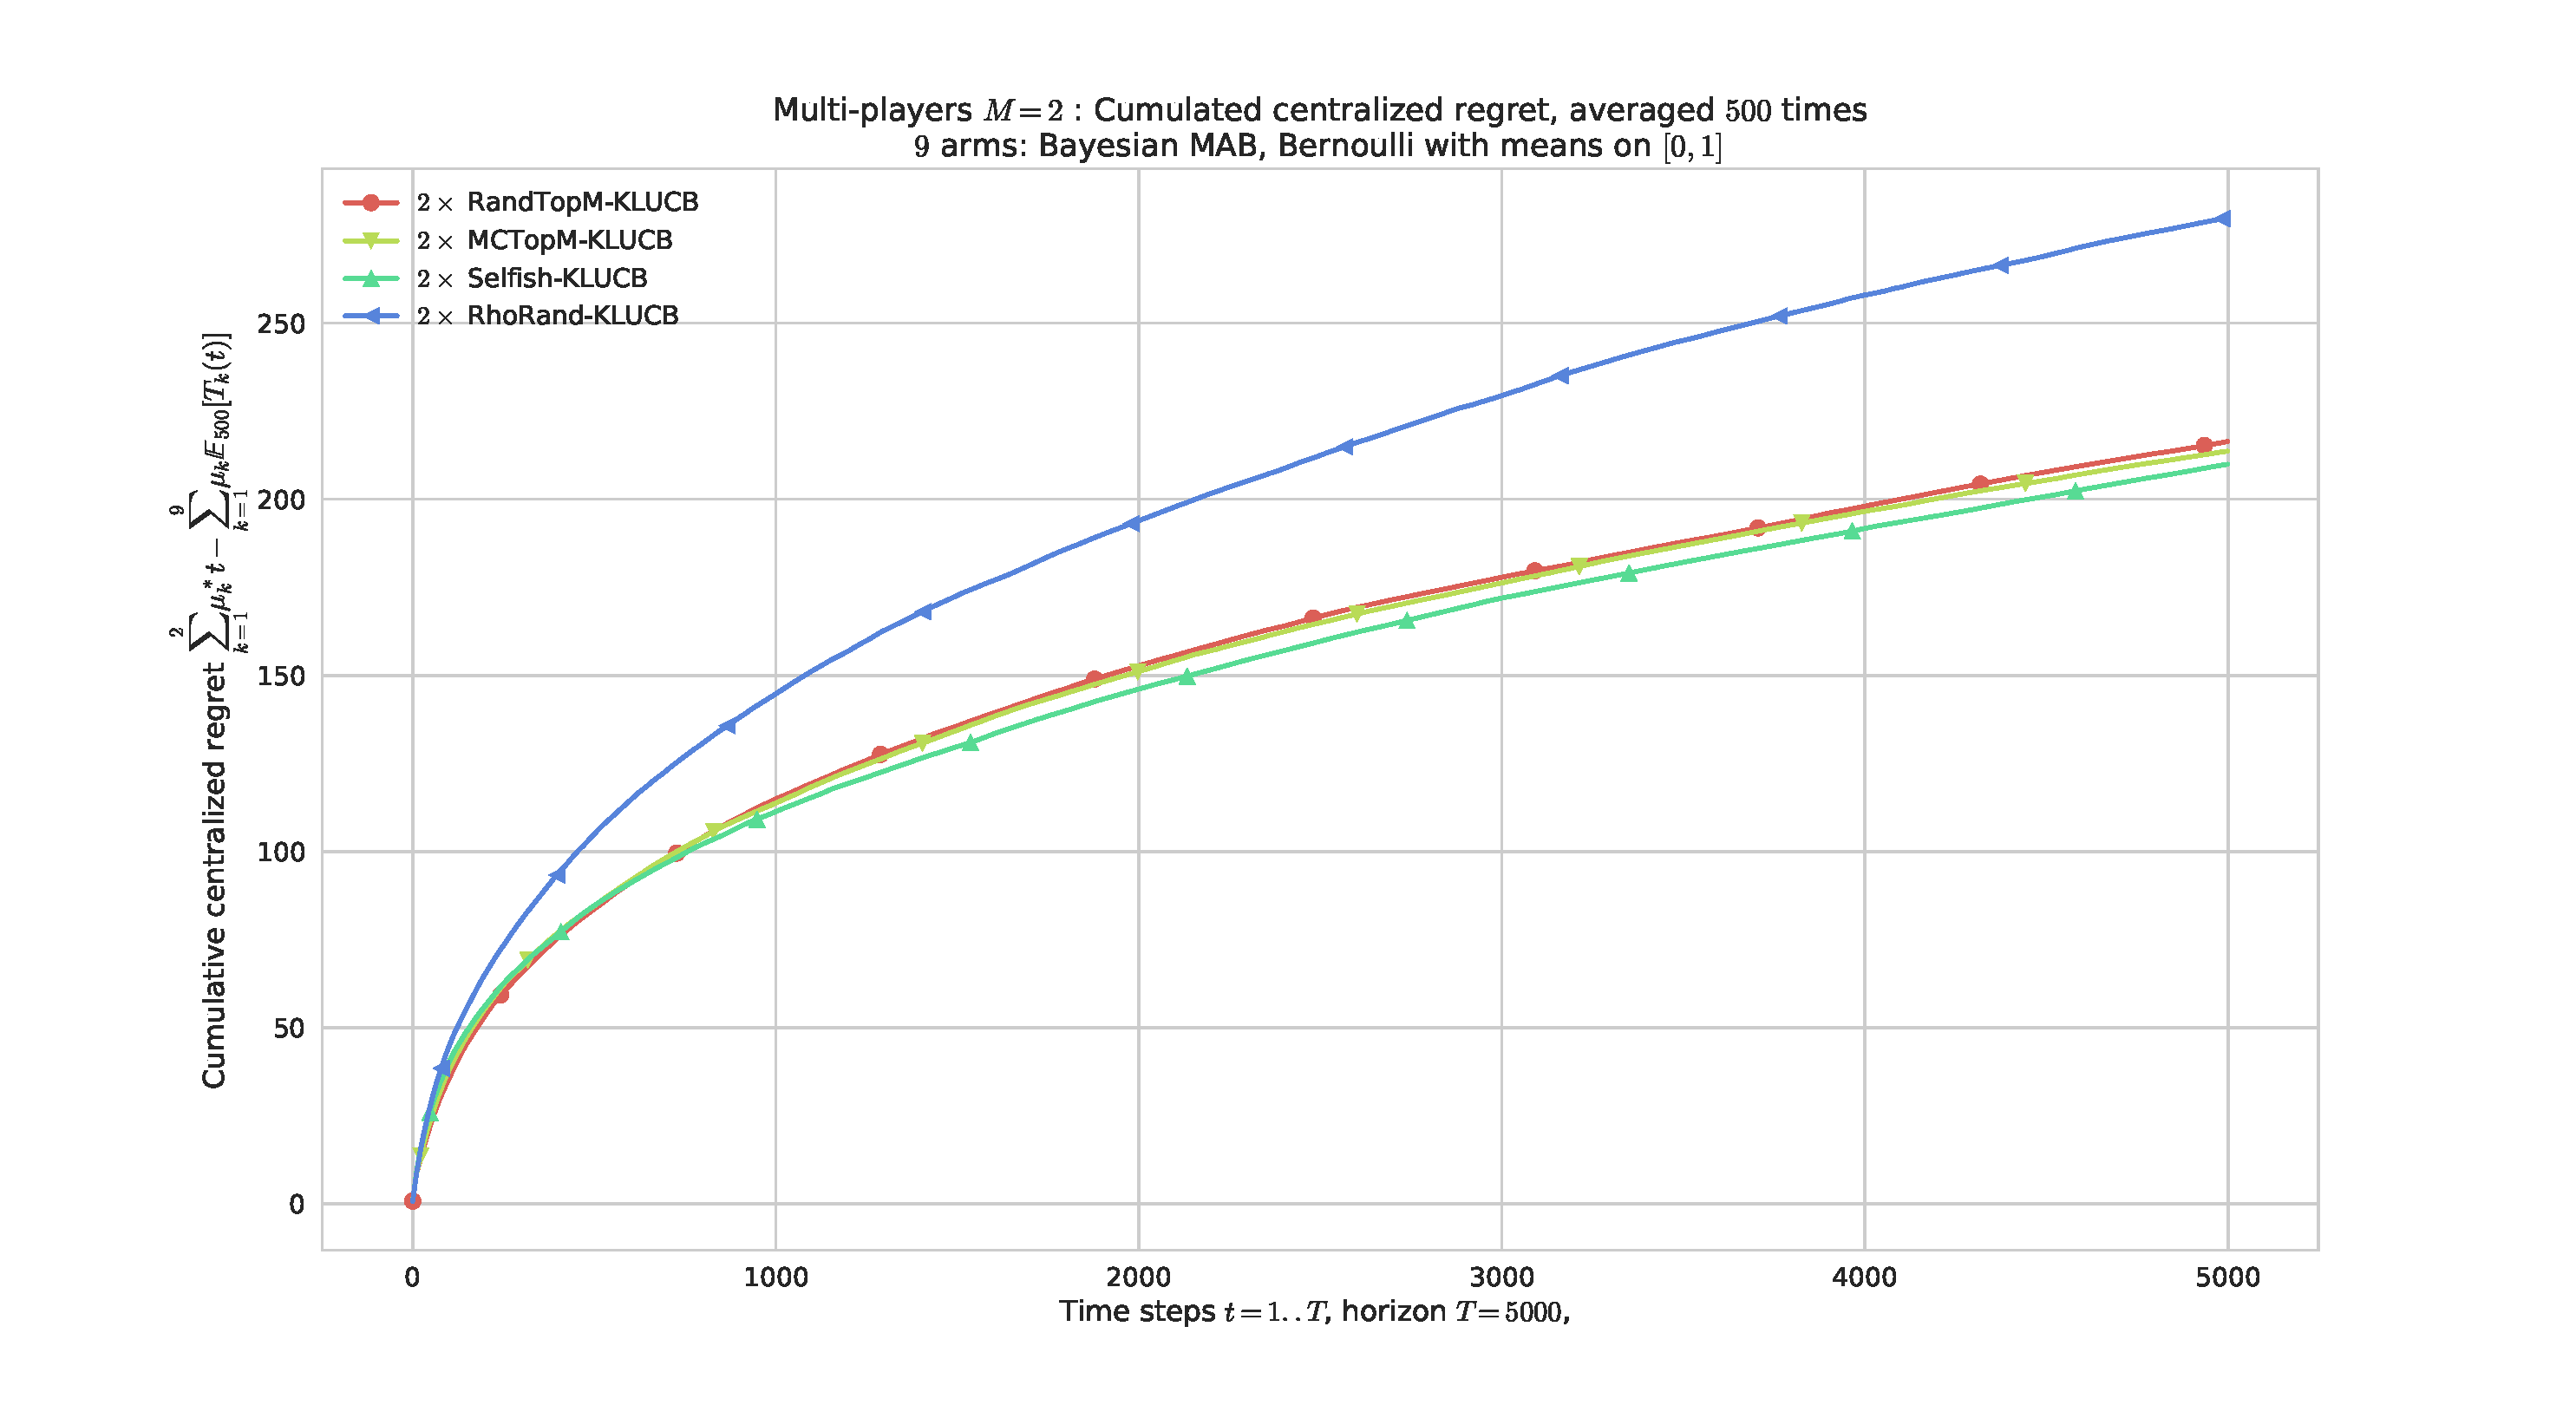
\includegraphics[width=1.00\textwidth]{MP__K9_M2_T5000_N500__4_algos/all_RegretCentralized____env1-1_3251433209347345969.pdf}
  % \end{subfigure}
  % ~
  % \begin{subfigure}[!h]{1.00\textwidth}
      % 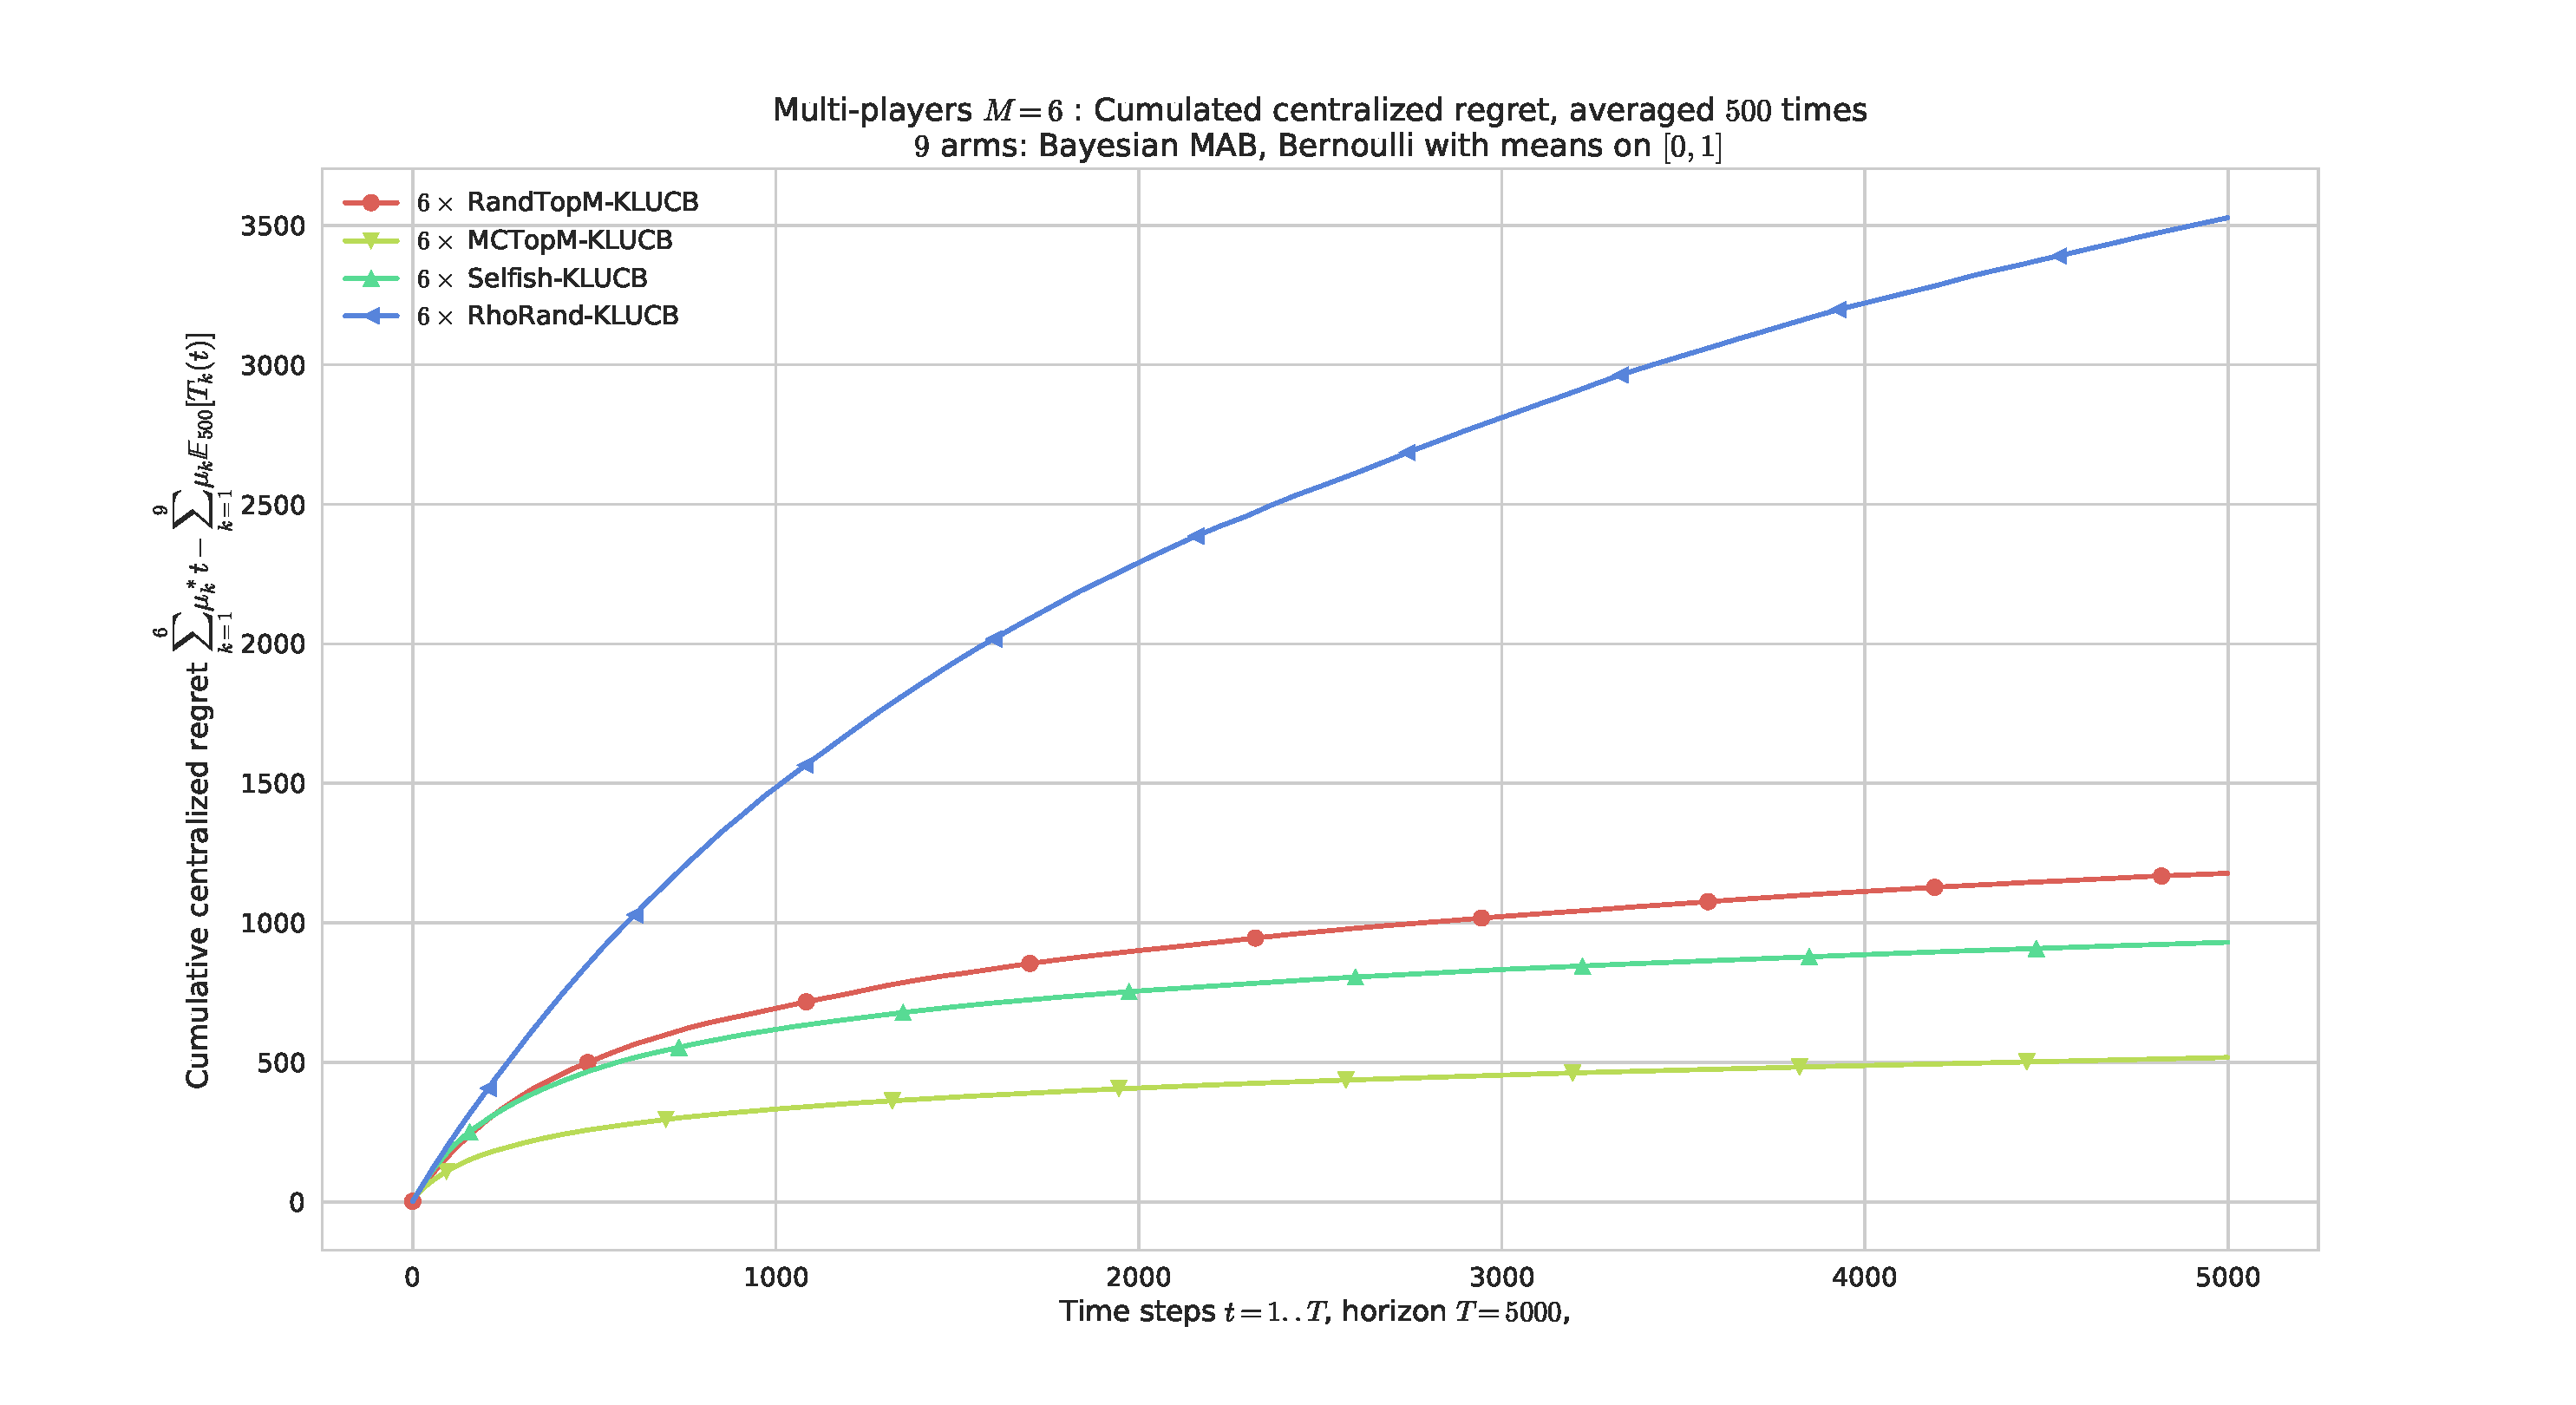
\includegraphics[width=1.00\textwidth]{MP__K9_M6_T5000_N500__4_algos/all_RegretCentralized____env1-1_8318947830261751207.pdf}
      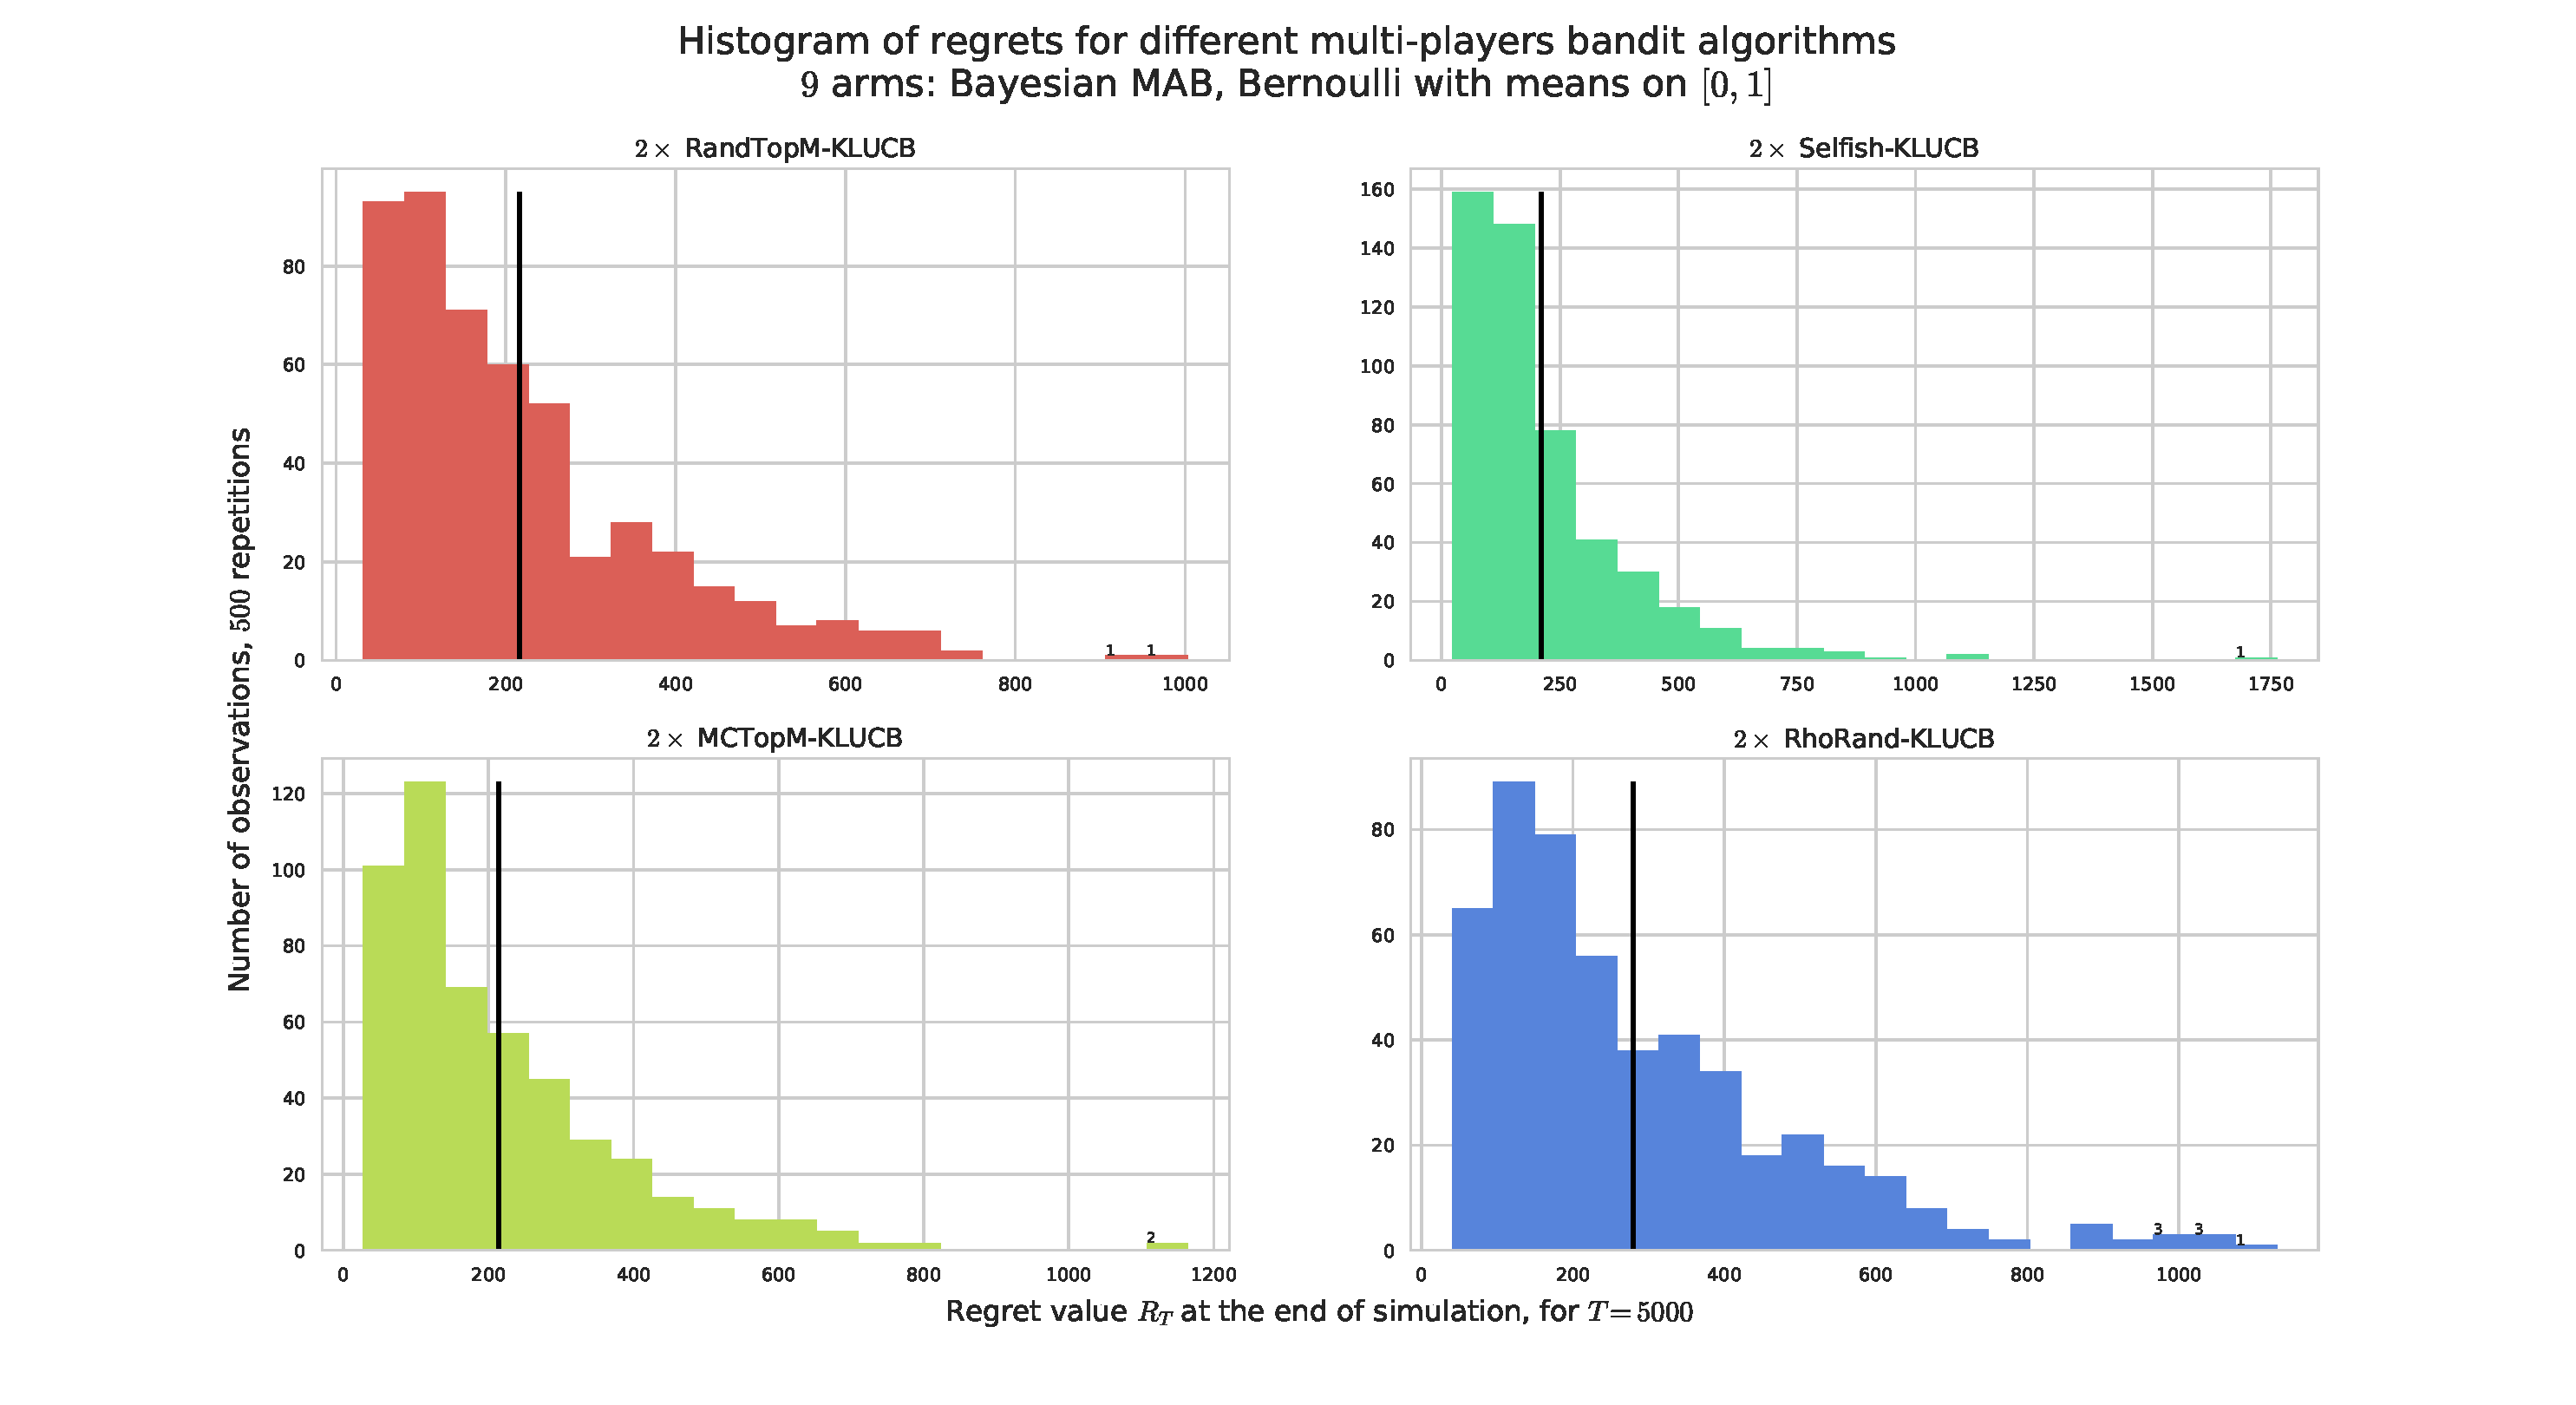
\includegraphics[width=1.00\textwidth]{MP__K9_M2_T5000_N500__4_algos/all_HistogramsRegret____env1-1_3251433209347345969.pdf}
  % \end{subfigure}
  \caption[Regret for $M=2$ players, $K=9$ arms, horizon $T=5000$, against $500$ problems $\boldsymbol{\mu}$ uniformly sampled]{Regret for $M=2$ players, $K=9$ arms, horizon $T=5000$, against $500$ problems $\boldsymbol{\mu}$ uniformly sampled in $[0,1]^K$. \rhoRand{} (top \textcolor{blue}{blue}) is outperformed by the other algorithms (and the gain increases when $M$ increases), which all perform similarly in such configurations. Note that the (small) tail of the histograms come from complicated problems $\boldsymbol{\mu}$ and not failure cases.}
  \label{fig:5:MP__K9_M2_T5000_N500__4_algos__all_RegretCentralized__BayesianProblems}
  % \vspace*{-15pt}  % XXX remove if problem
\end{figure}


\begin{figure}[!h]
  \centering
  % \begin{subfigure}[!h]{1.00\textwidth}
      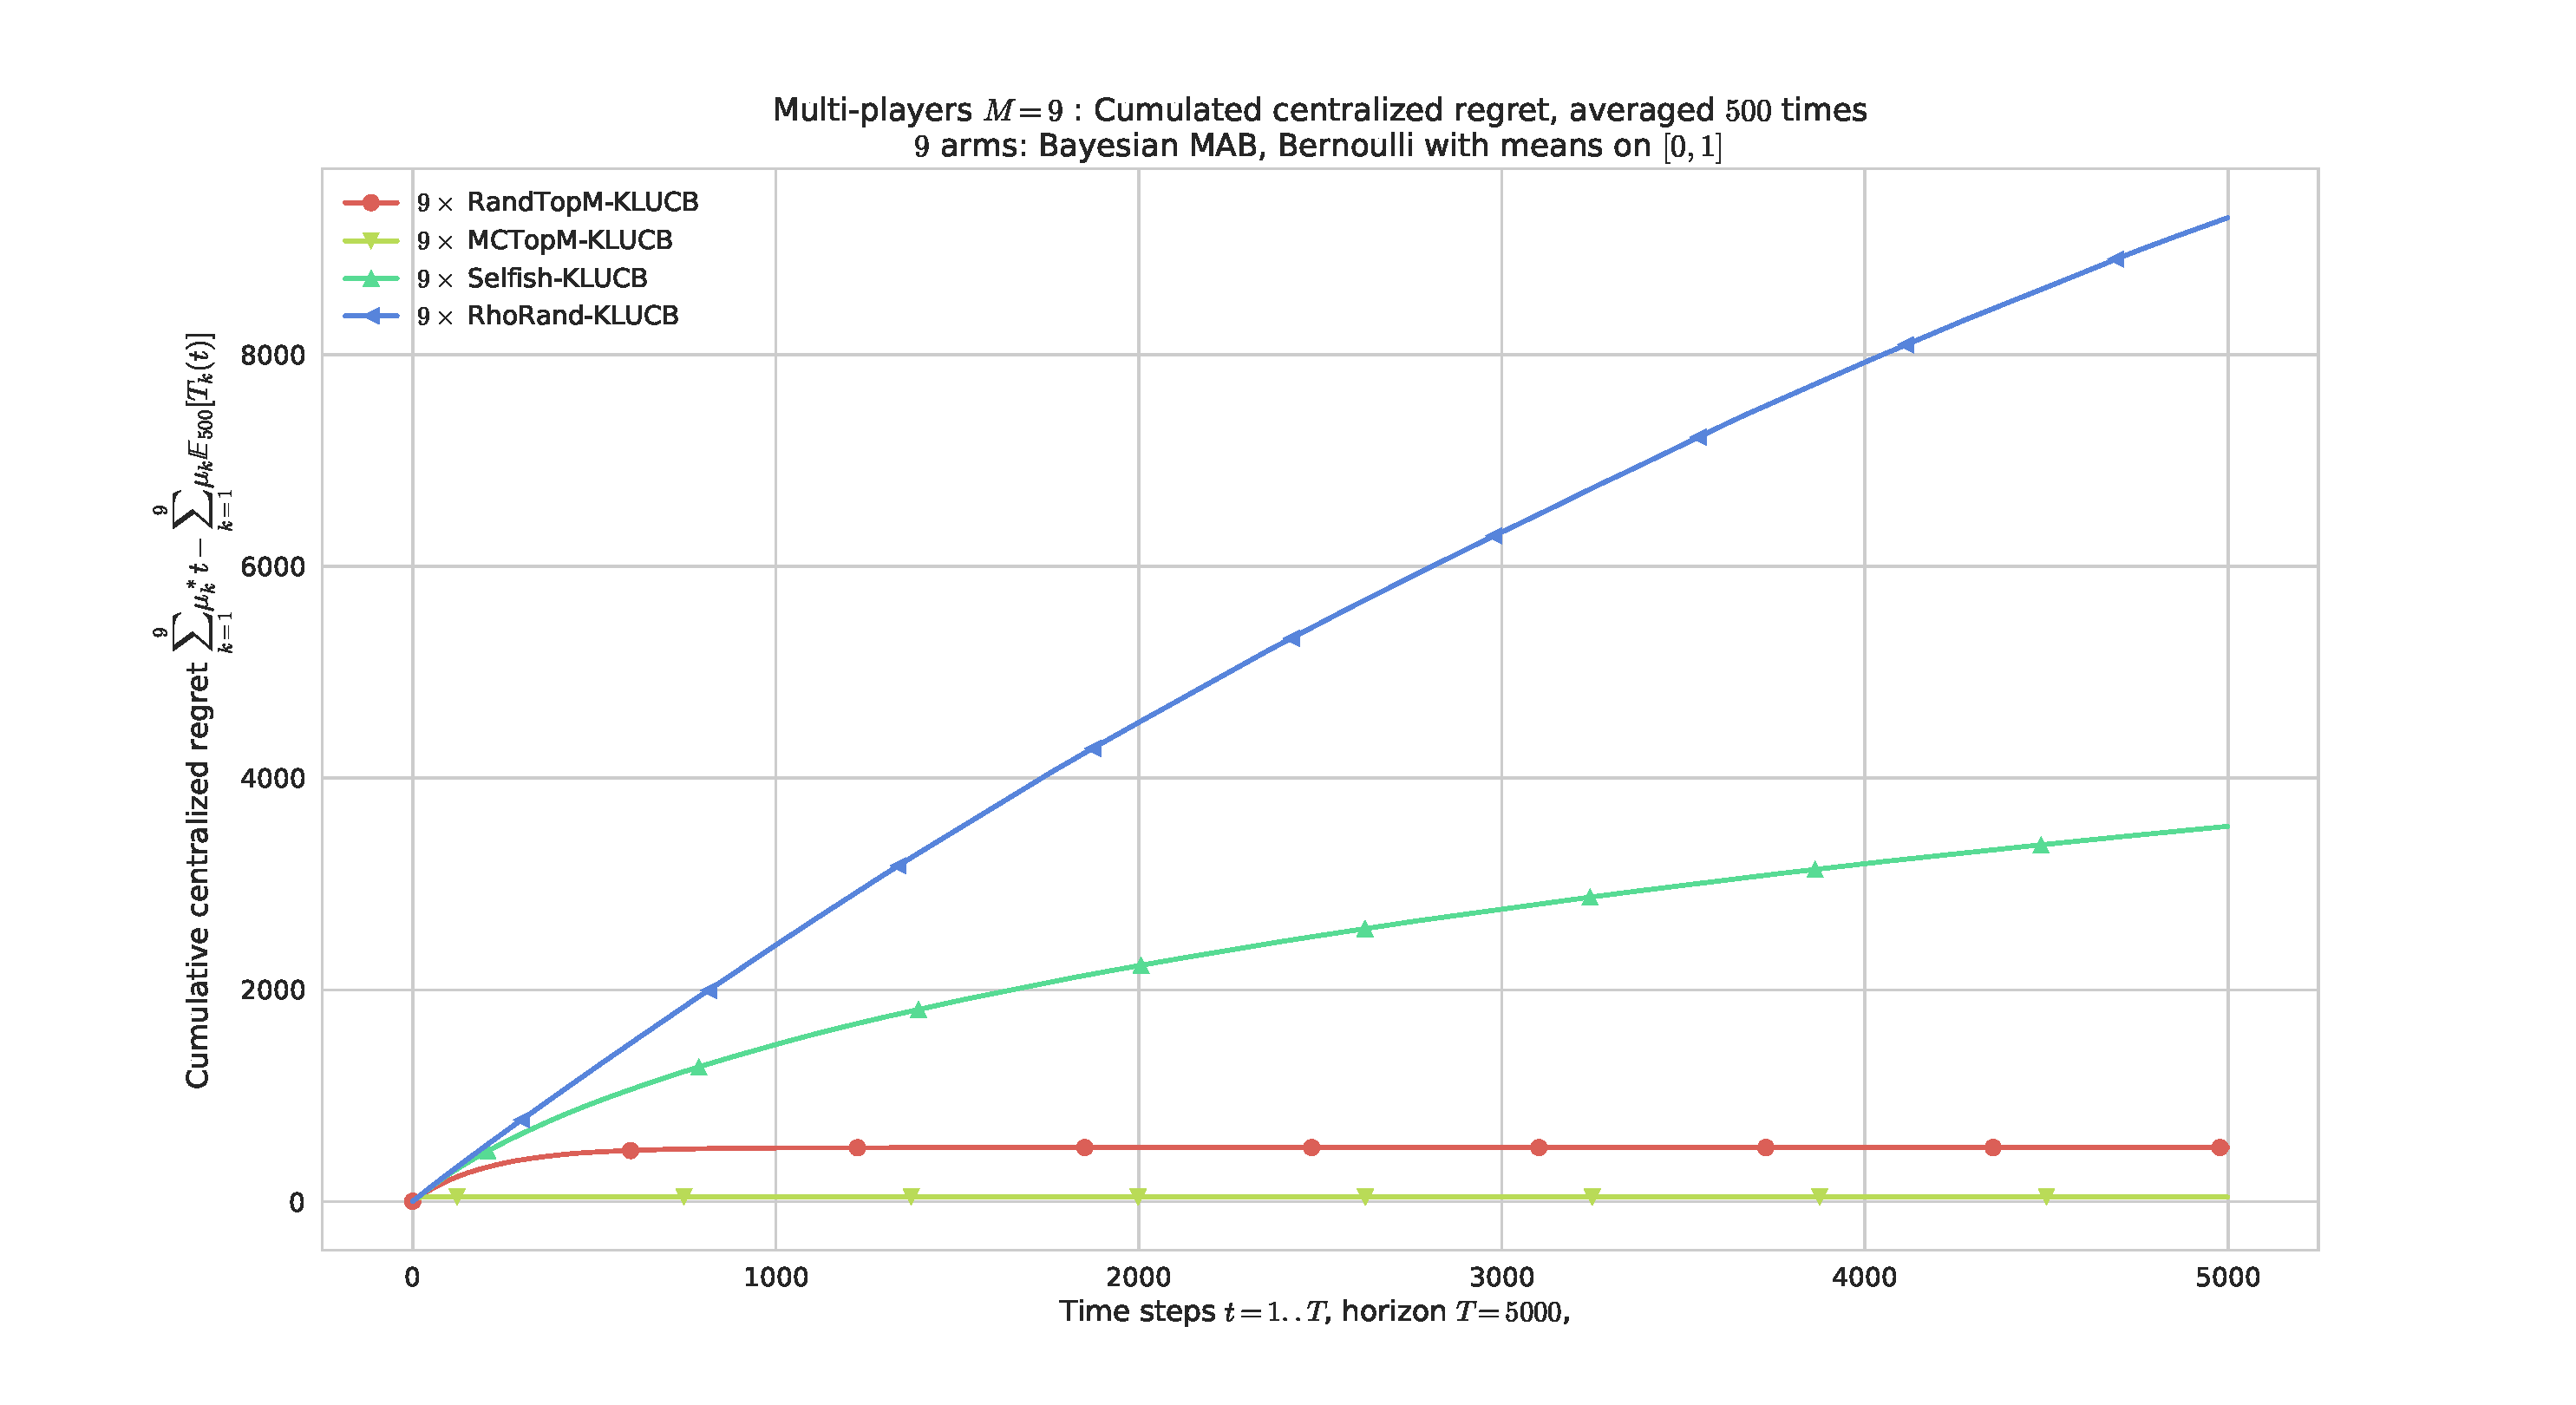
\includegraphics[width=1.00\textwidth]{MP__K9_M9_T5000_N500__4_algos/all_RegretCentralized____env1-1_3892966382091165662.pdf}
  % \end{subfigure}
  % ~
  % \begin{subfigure}[!h]{1.00\textwidth}
      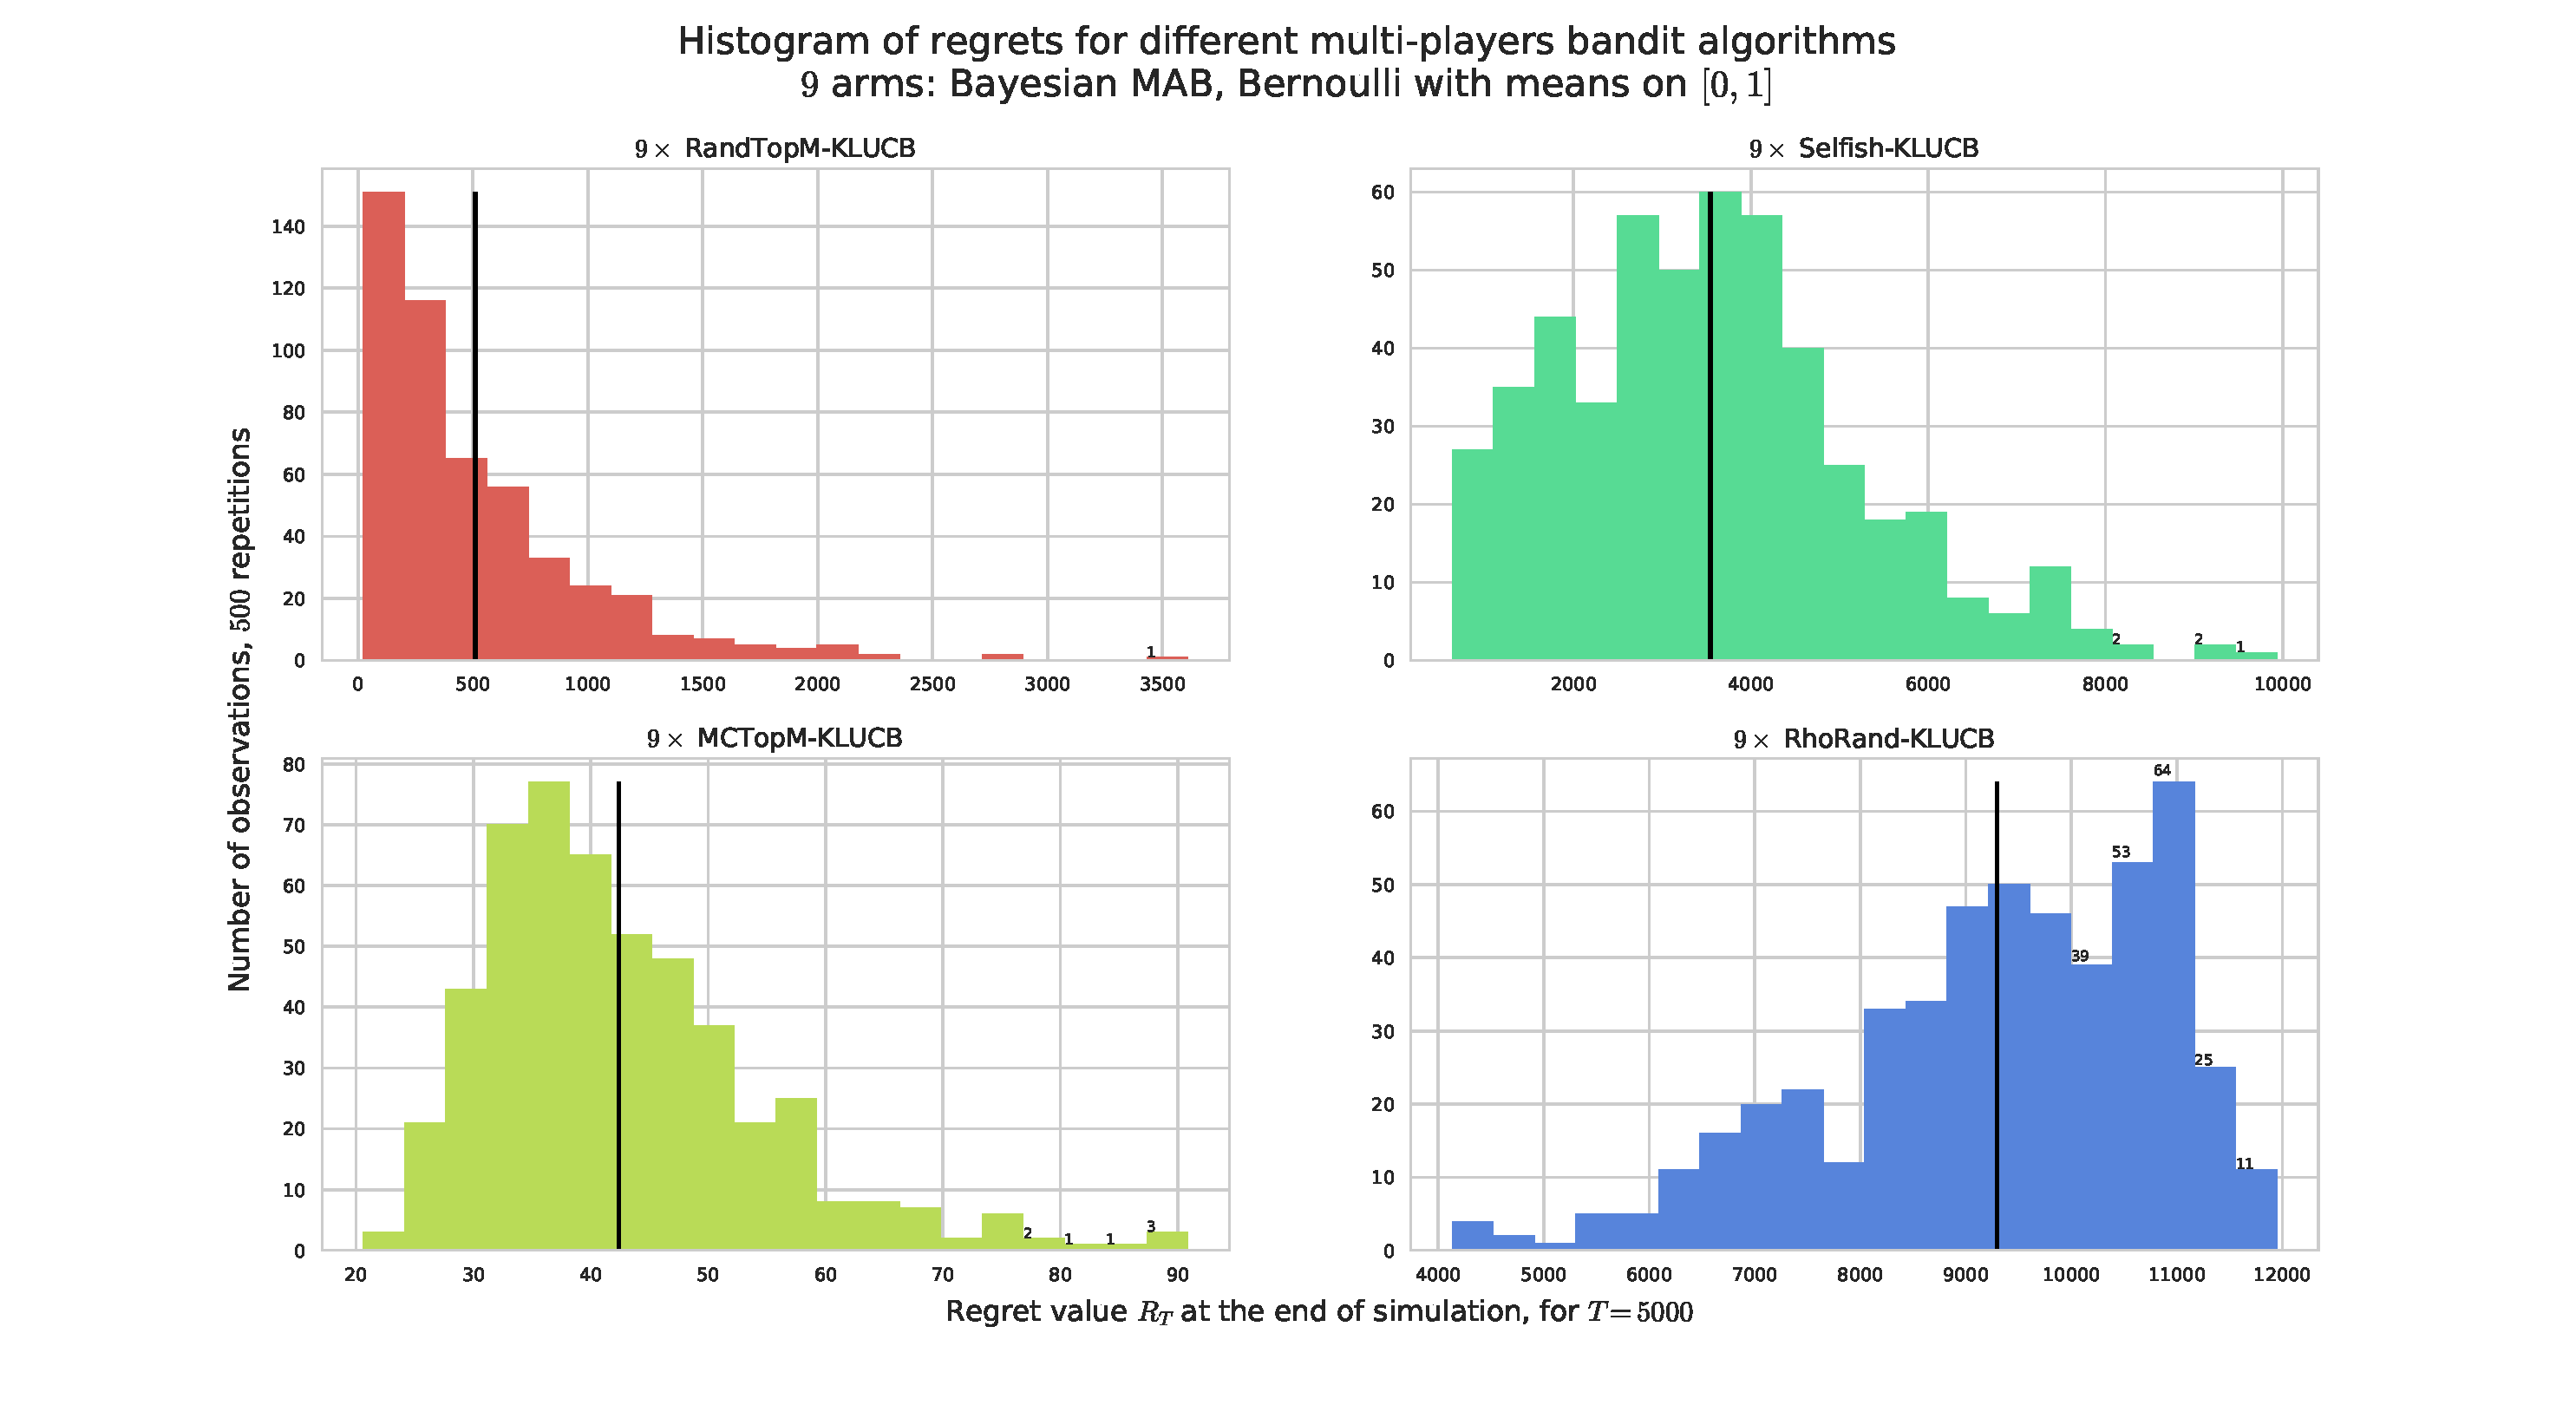
\includegraphics[width=1.00\textwidth]{MP__K9_M9_T5000_N500__4_algos/all_HistogramsRegret____env1-1_3892966382091165662.pdf}
  % \end{subfigure}
  \caption[Regret for $M=9$ players for $K=9$ arms, horizon $T=5000$, against $500$ problems $\boldsymbol{\mu}$ uniformly sampled]{Regret for $M=9$ players for $K=9$ arms, horizon $T=5000$, against $500$ problems $\boldsymbol{\mu}$ uniformly sampled in $[0,1]^K$. This extreme case $M=K$ shows the drastic difference of behavior between \RandTopM{} and \MCTopM, having constant regret, and \rhoRand{} and \Selfish, having large regret.}
  \label{fig:5:MP__K9_M9_T5000_N500__4_algos__all_HistogramsRegret}
  % \vspace*{-15pt}  % XXX remove if problem
\end{figure}


\begin{figure}[!h]
  \centering
  % \begin{subfigure}[!h]{1.00\textwidth}
      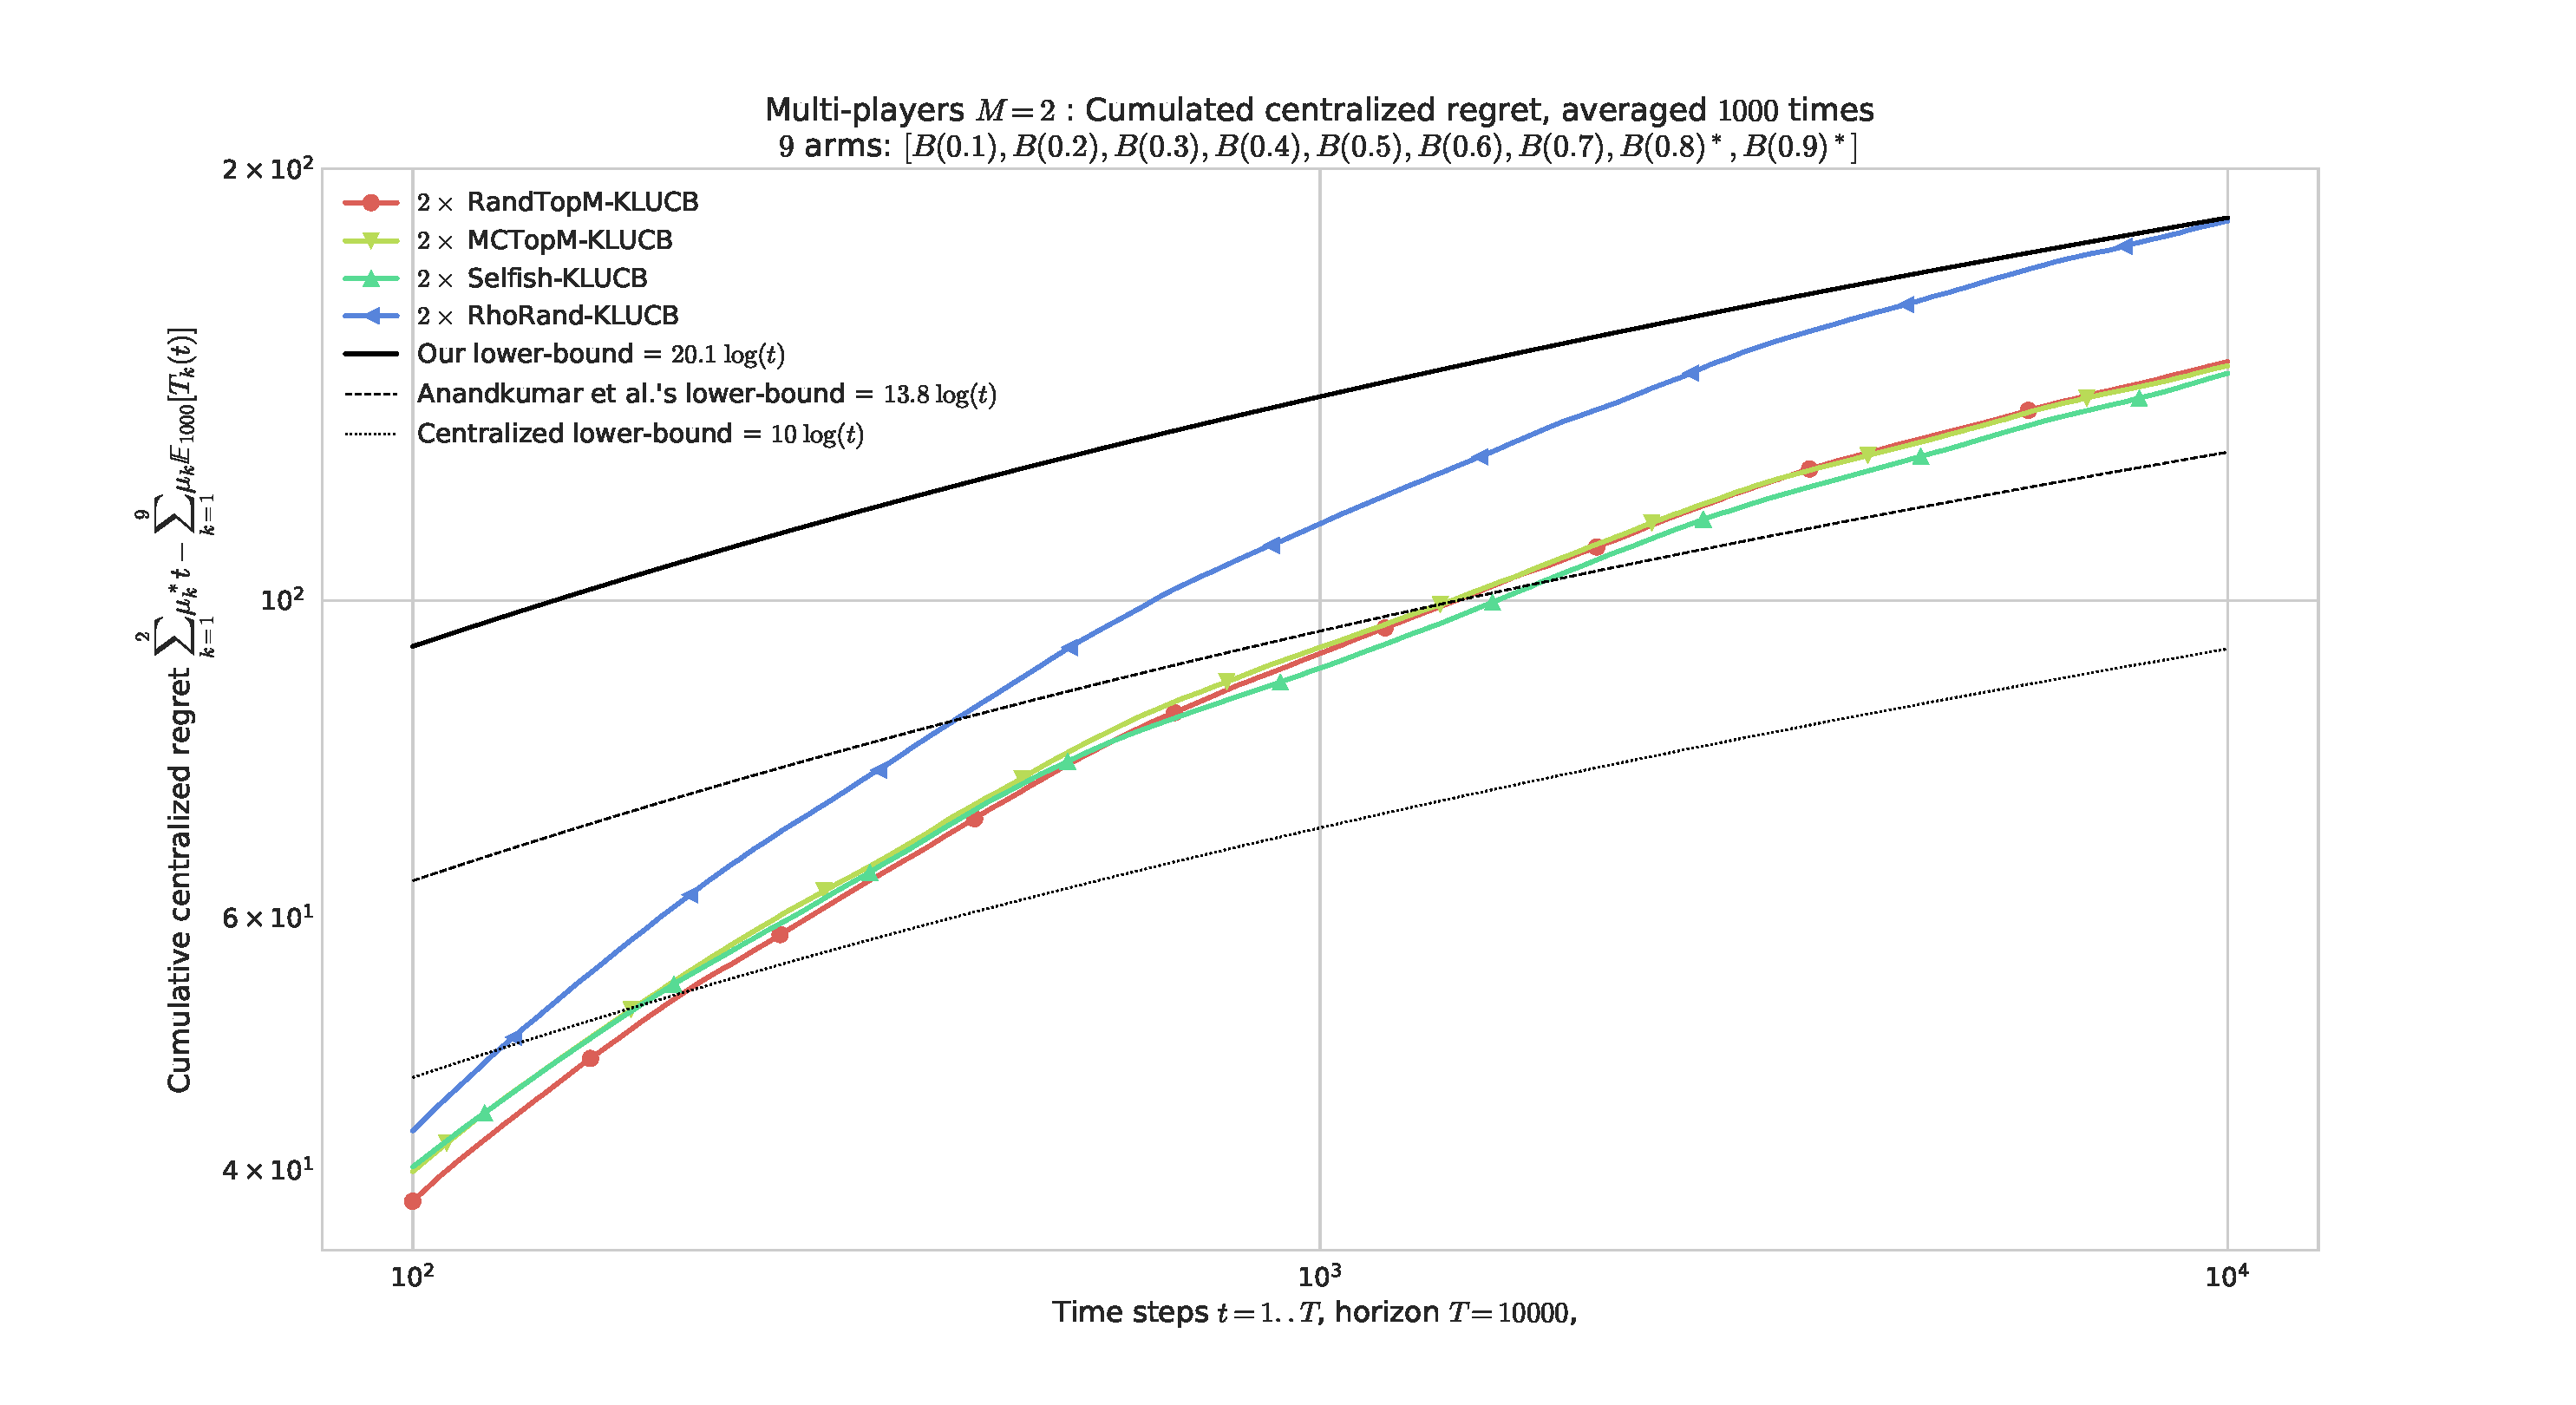
\includegraphics[width=1.00\textwidth]{MP__K9_M2_T10000_N1000__4_algos/all_RegretCentralized_loglog____env1-1_2643359116089264295.pdf}
  % \end{subfigure}
  % ~
  % \begin{subfigure}[!h]{1.00\textwidth}
  %   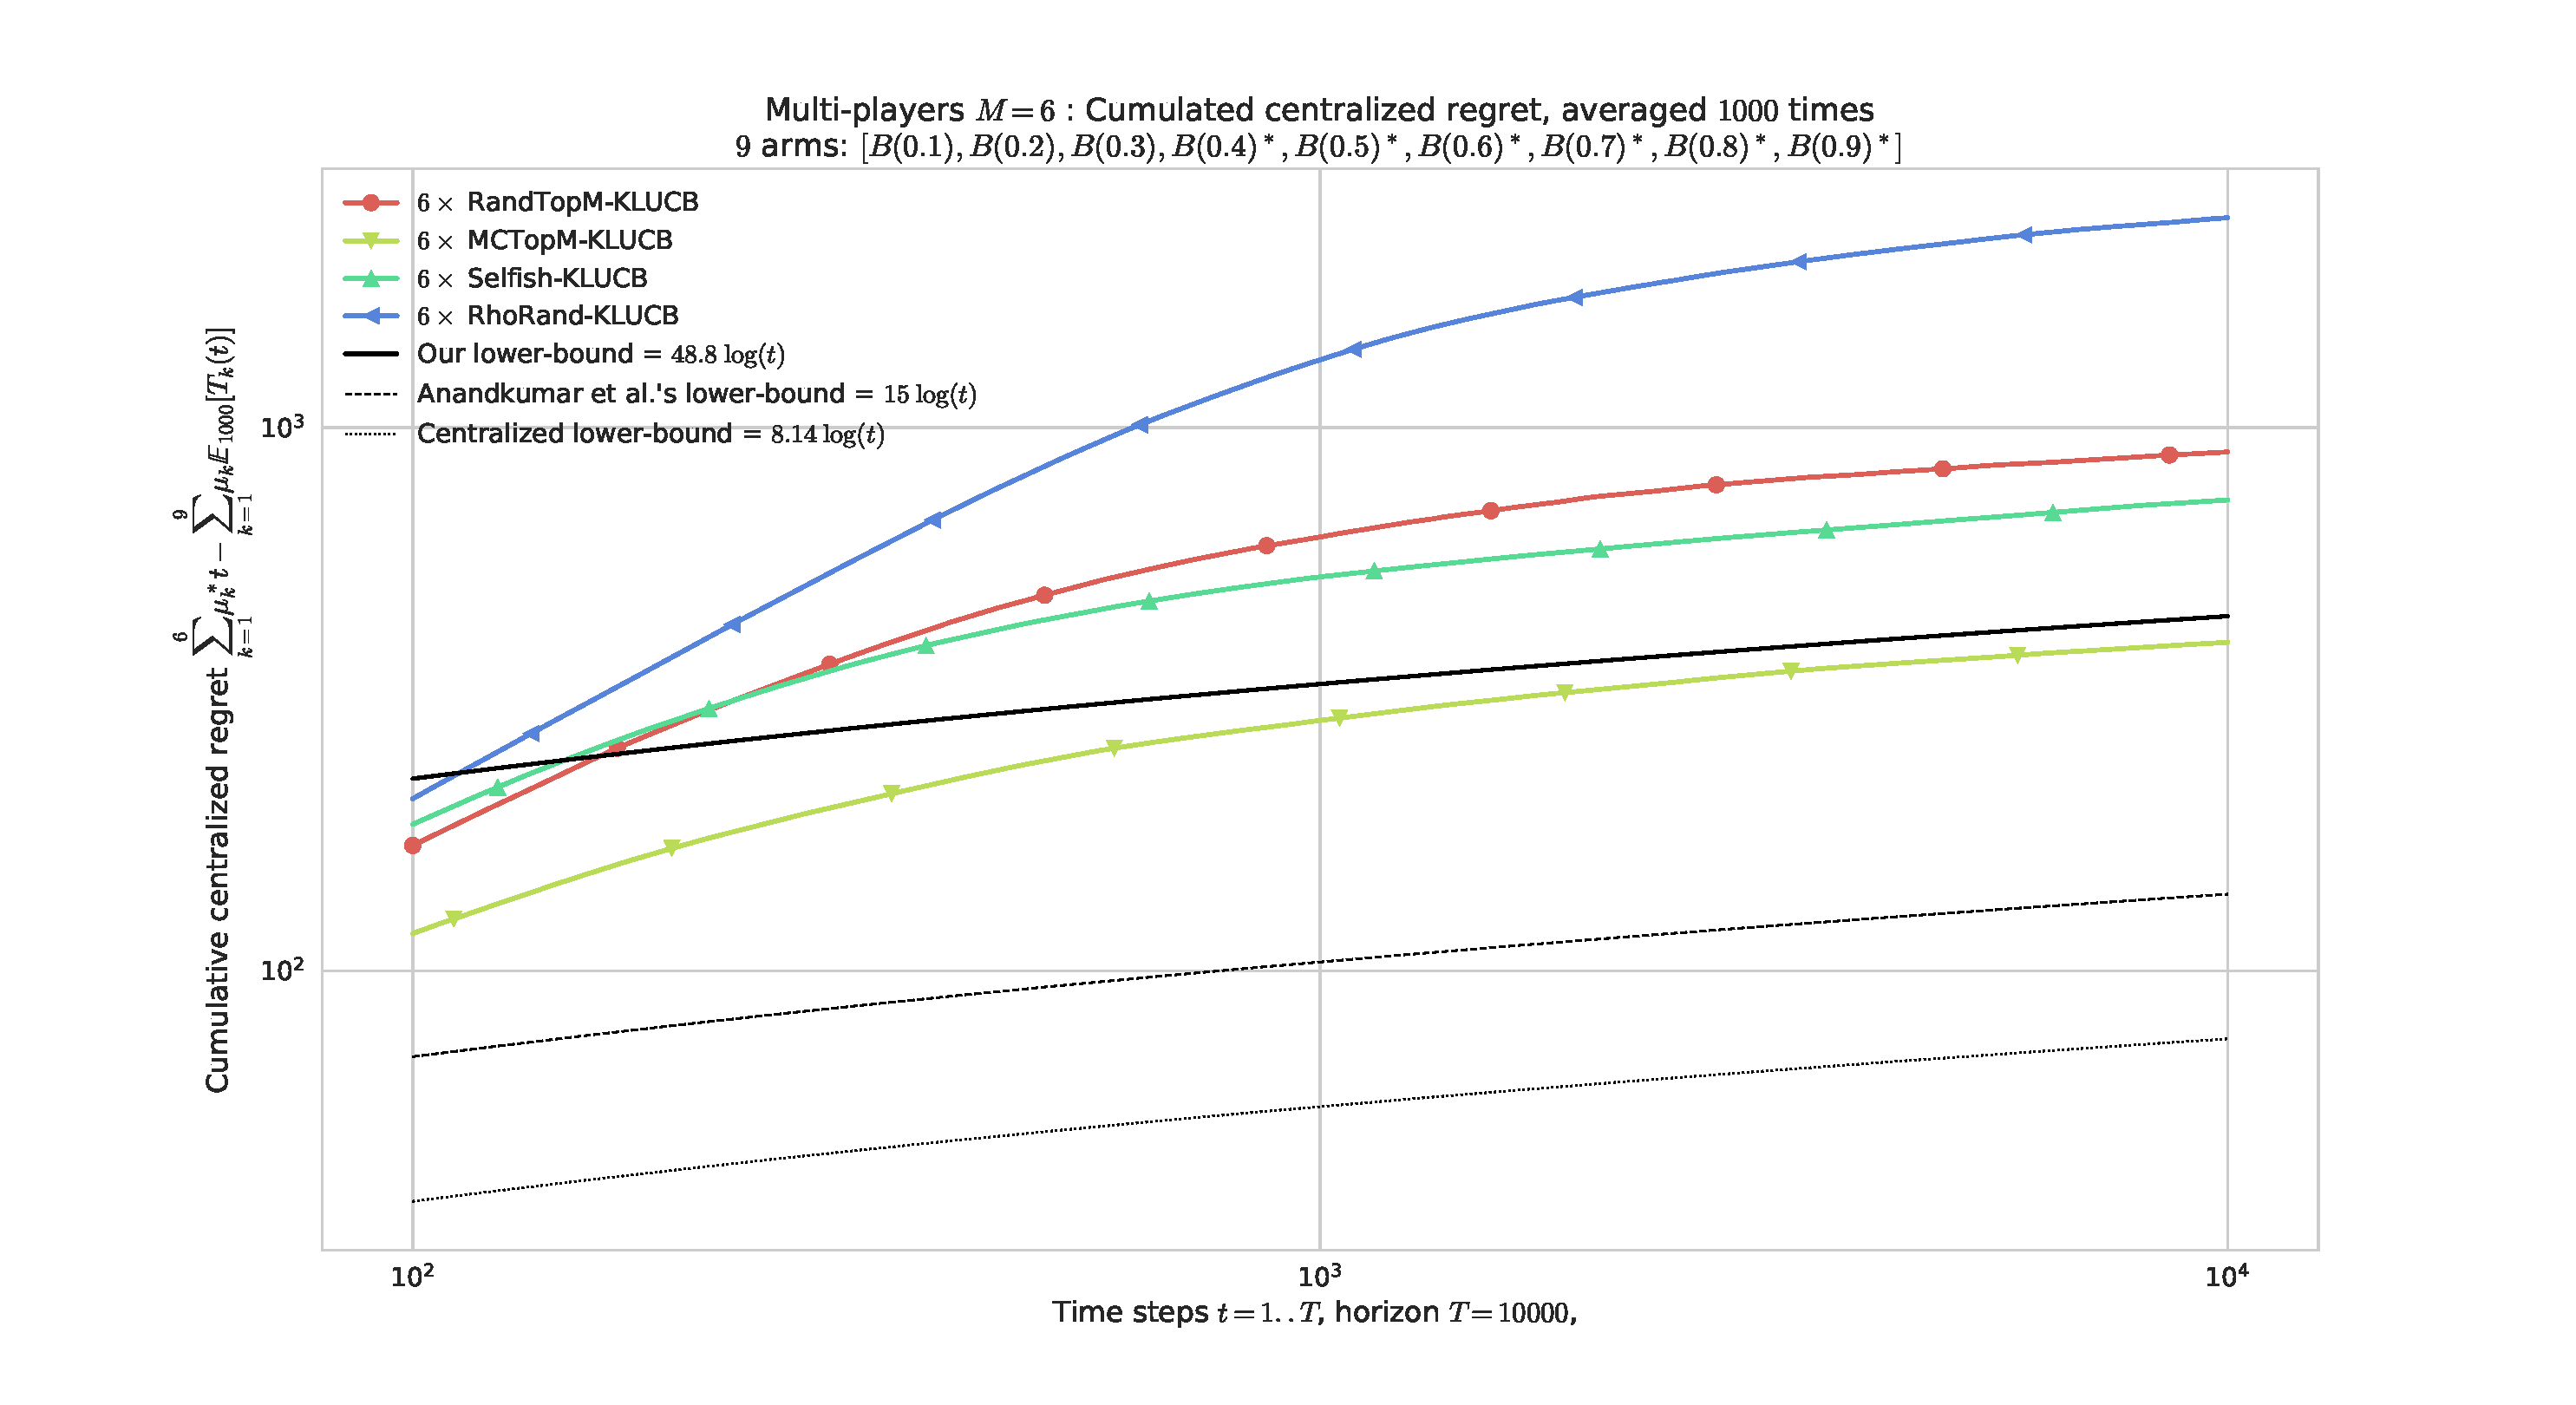
\includegraphics[width=1.00\textwidth]{MP__K9_M6_T10000_N1000__4_algos/all_RegretCentralized_loglog____env1-1_8200873569864822246.pdf}
  % \end{subfigure}
  % ~
  % \begin{subfigure}[!h]{1.00\textwidth}
      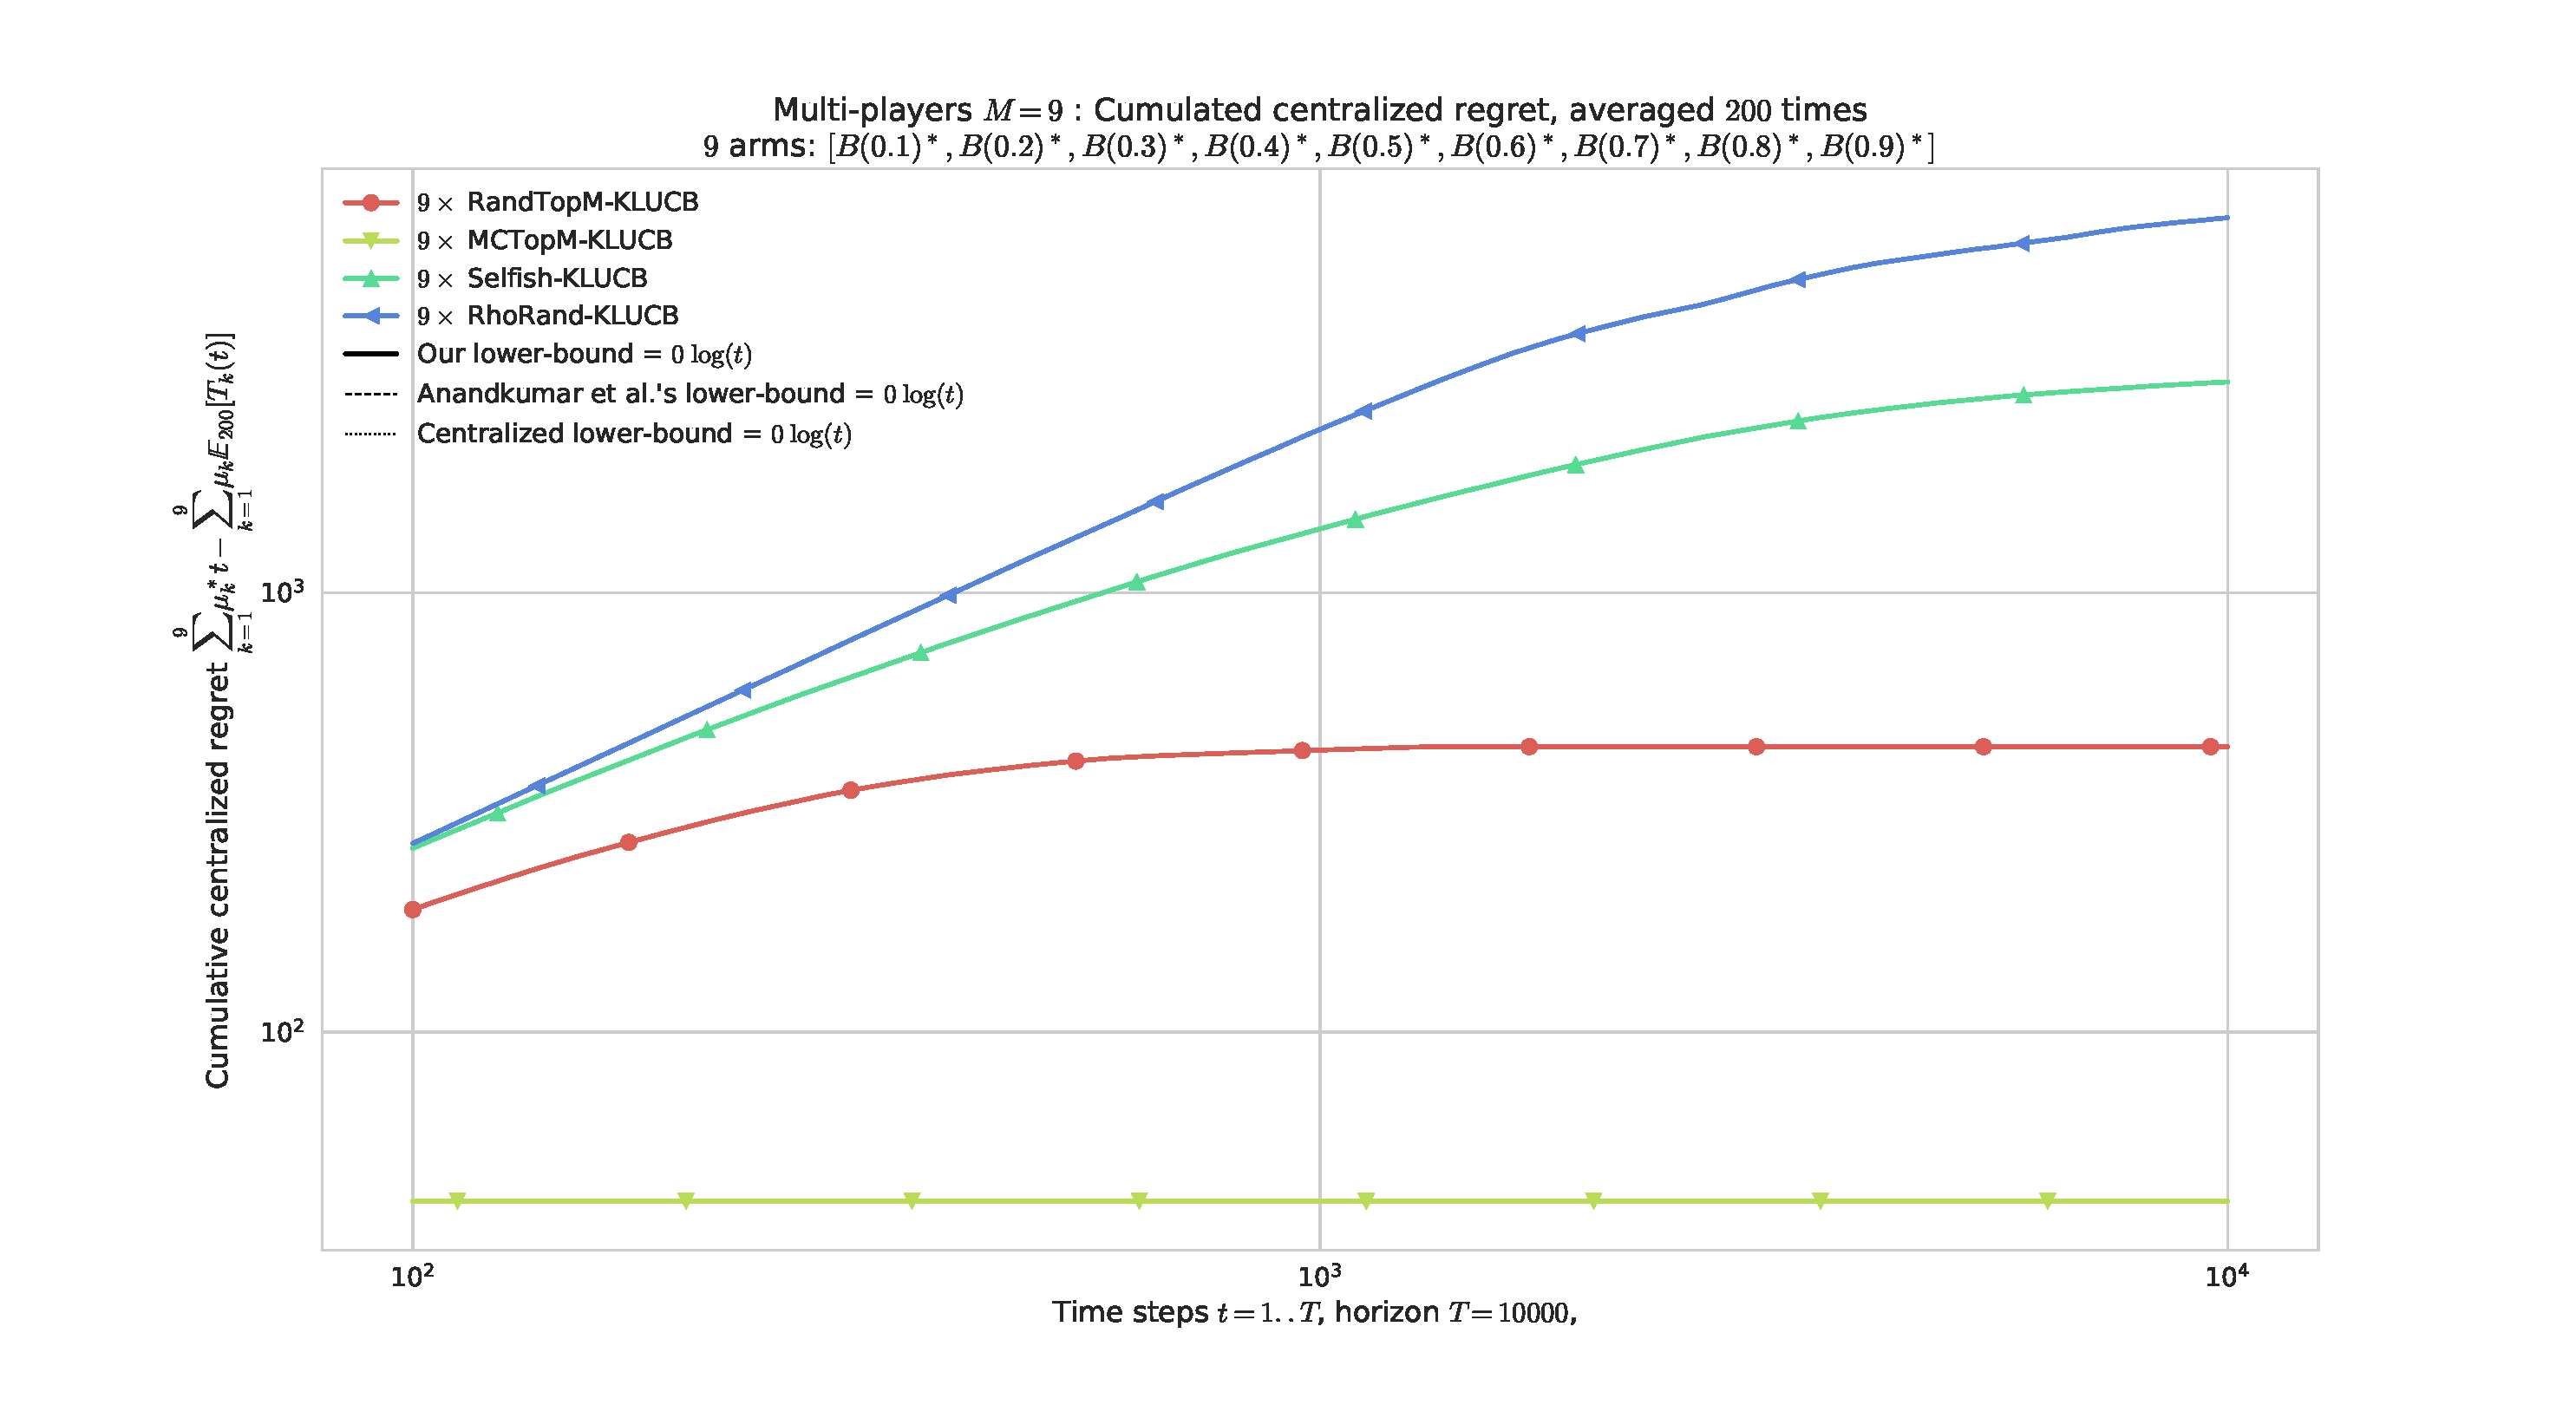
\includegraphics[width=1.00\textwidth]{MP__K9_M9_T10000_N200__4_algos/all_RegretCentralized_loglog____env1-1_2306423191427933958.pdf}
  % \end{subfigure}
  \caption[Regret for $M=2$ and $9$ players for $K=9$ arms, horizon $T=5000$, for a fixed problem]{Regret (in log-log scale), for $M=2$ and $9$ players for $K=9$ arms, horizon $T=5000$,Regret (in log-log scale), for $M=2$ and $9$ players for $K=9$ arms, horizon $T=5000$, for problem $\boldsymbol{\mu}=[0.1,\dots,0.9]$] for problem $\boldsymbol{\mu}=[0.1,\dots,0.9]$. In different settings, \RandTopM{} (\textcolor{gold}{yellow} curve) and \Selfish{} (\textcolor{darkgreen}{green}) can outperform each other, and always outperform \rhoRand. \MCTopM{} is always among the best algorithms, and for $M$ not too small, its regret seems logarithmic with a constant matching the lower bound.}
  \label{fig:5:MP__K9_M2-6-9_T10000_N200__4_algos}
\end{figure}


\begin{figure}[!h]
  \centering
  % \begin{subfigure}[!h]{0.75\textwidth}
      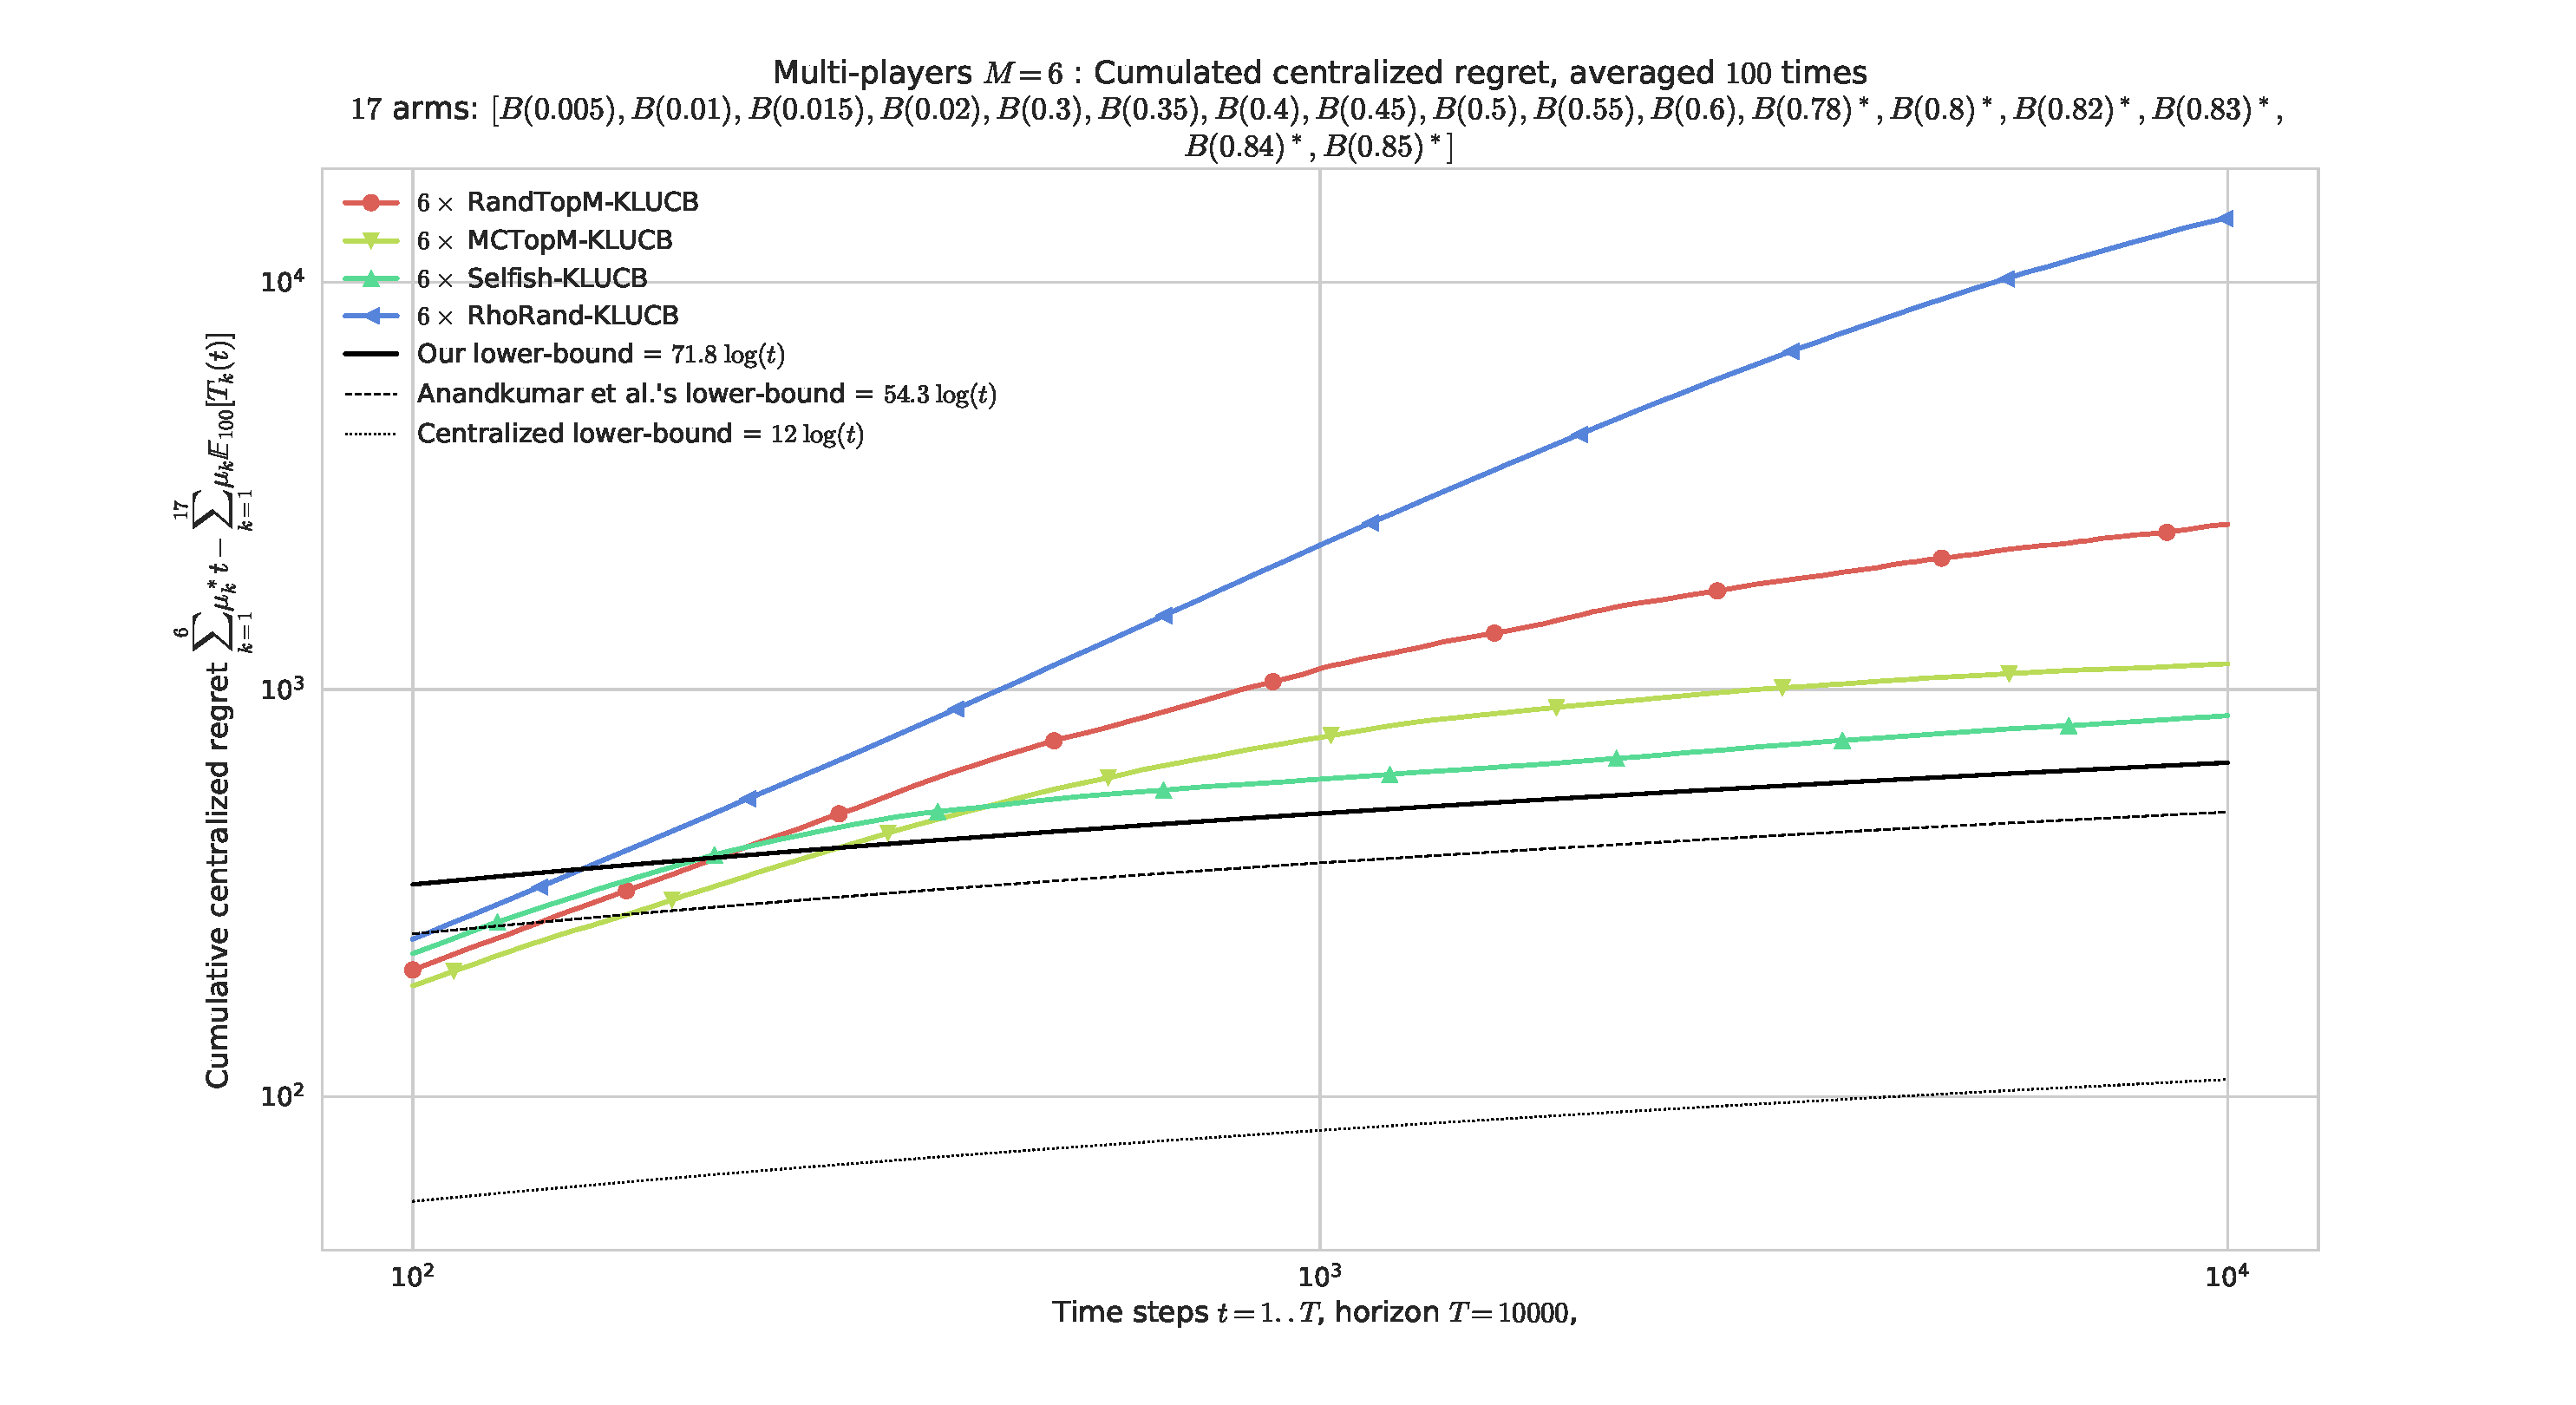
\includegraphics[width=1.00\textwidth]{MP__K17_M6_T10000_N100__4_algos/all_RegretCentralized_loglog____env1-1_4163066365888233475.pdf}
  % \end{subfigure}
  % ~
  % \begin{subfigure}[!h]{0.75\textwidth}
      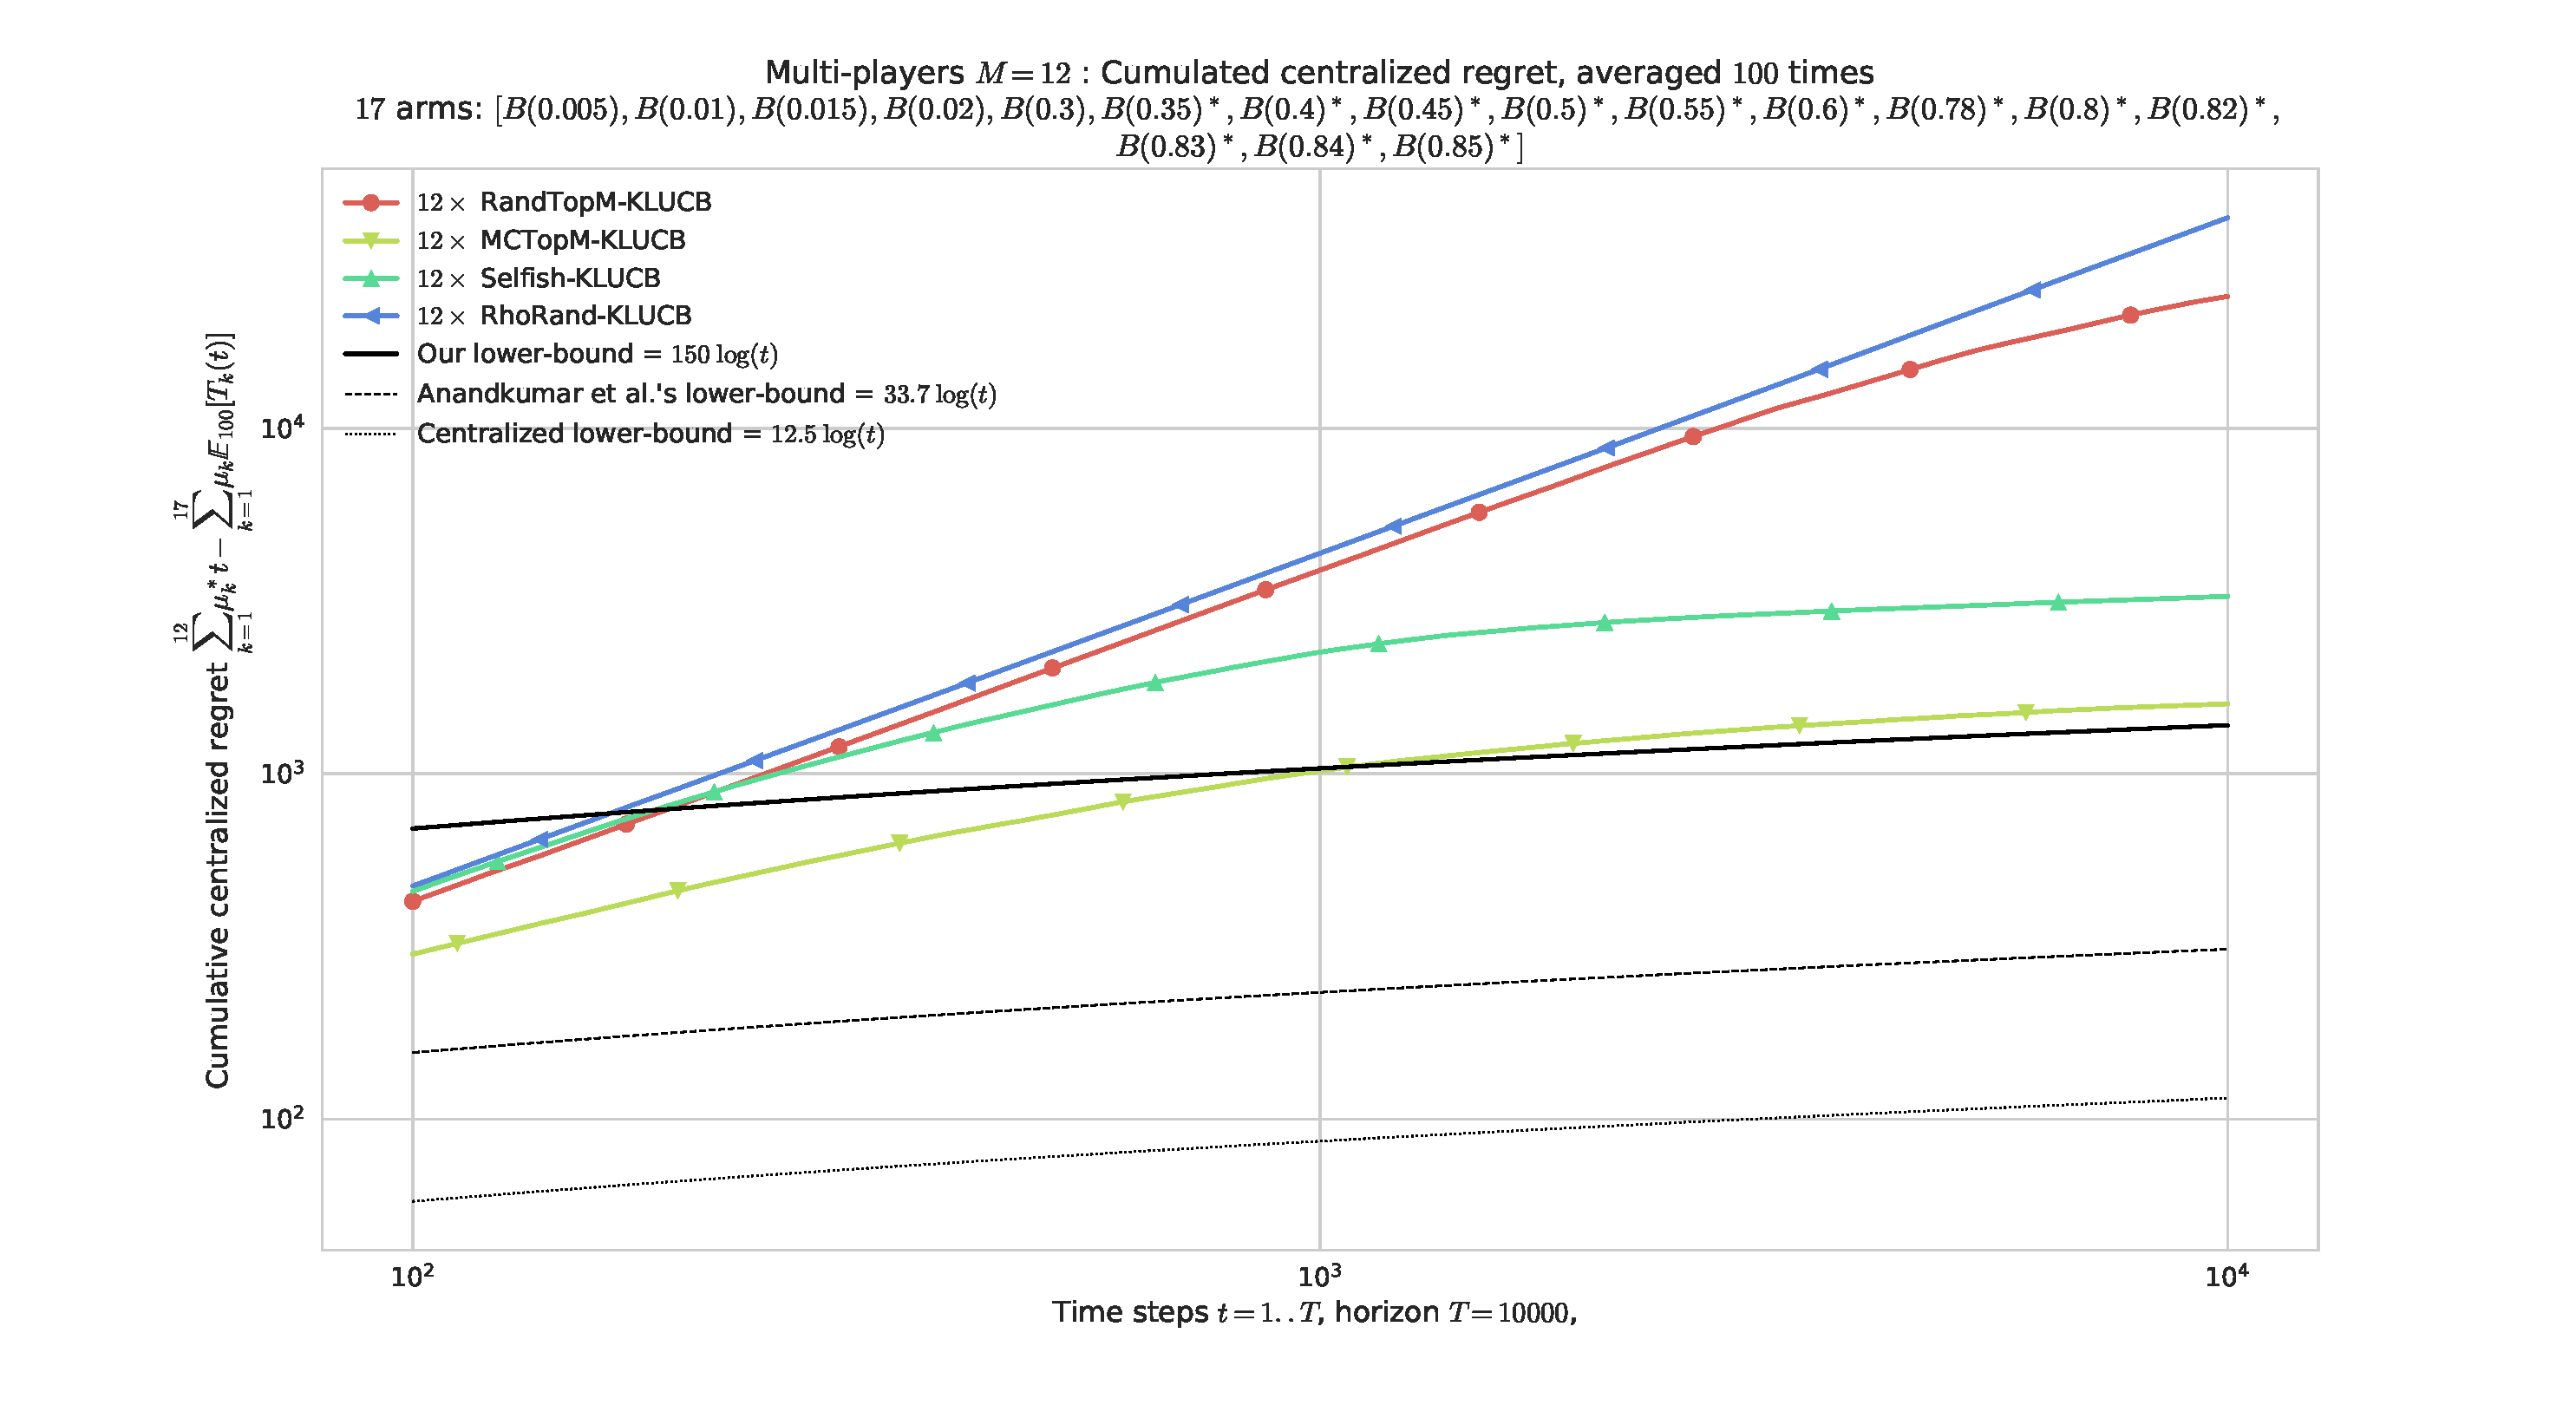
\includegraphics[width=1.00\textwidth]{MP__K17_M12_T10000_N100__4_algos/all_RegretCentralized_loglog____env1-1_3856003705095179548.pdf}
  % \end{subfigure}
  % ~
  % \begin{subfigure}[!h]{0.75\textwidth}
      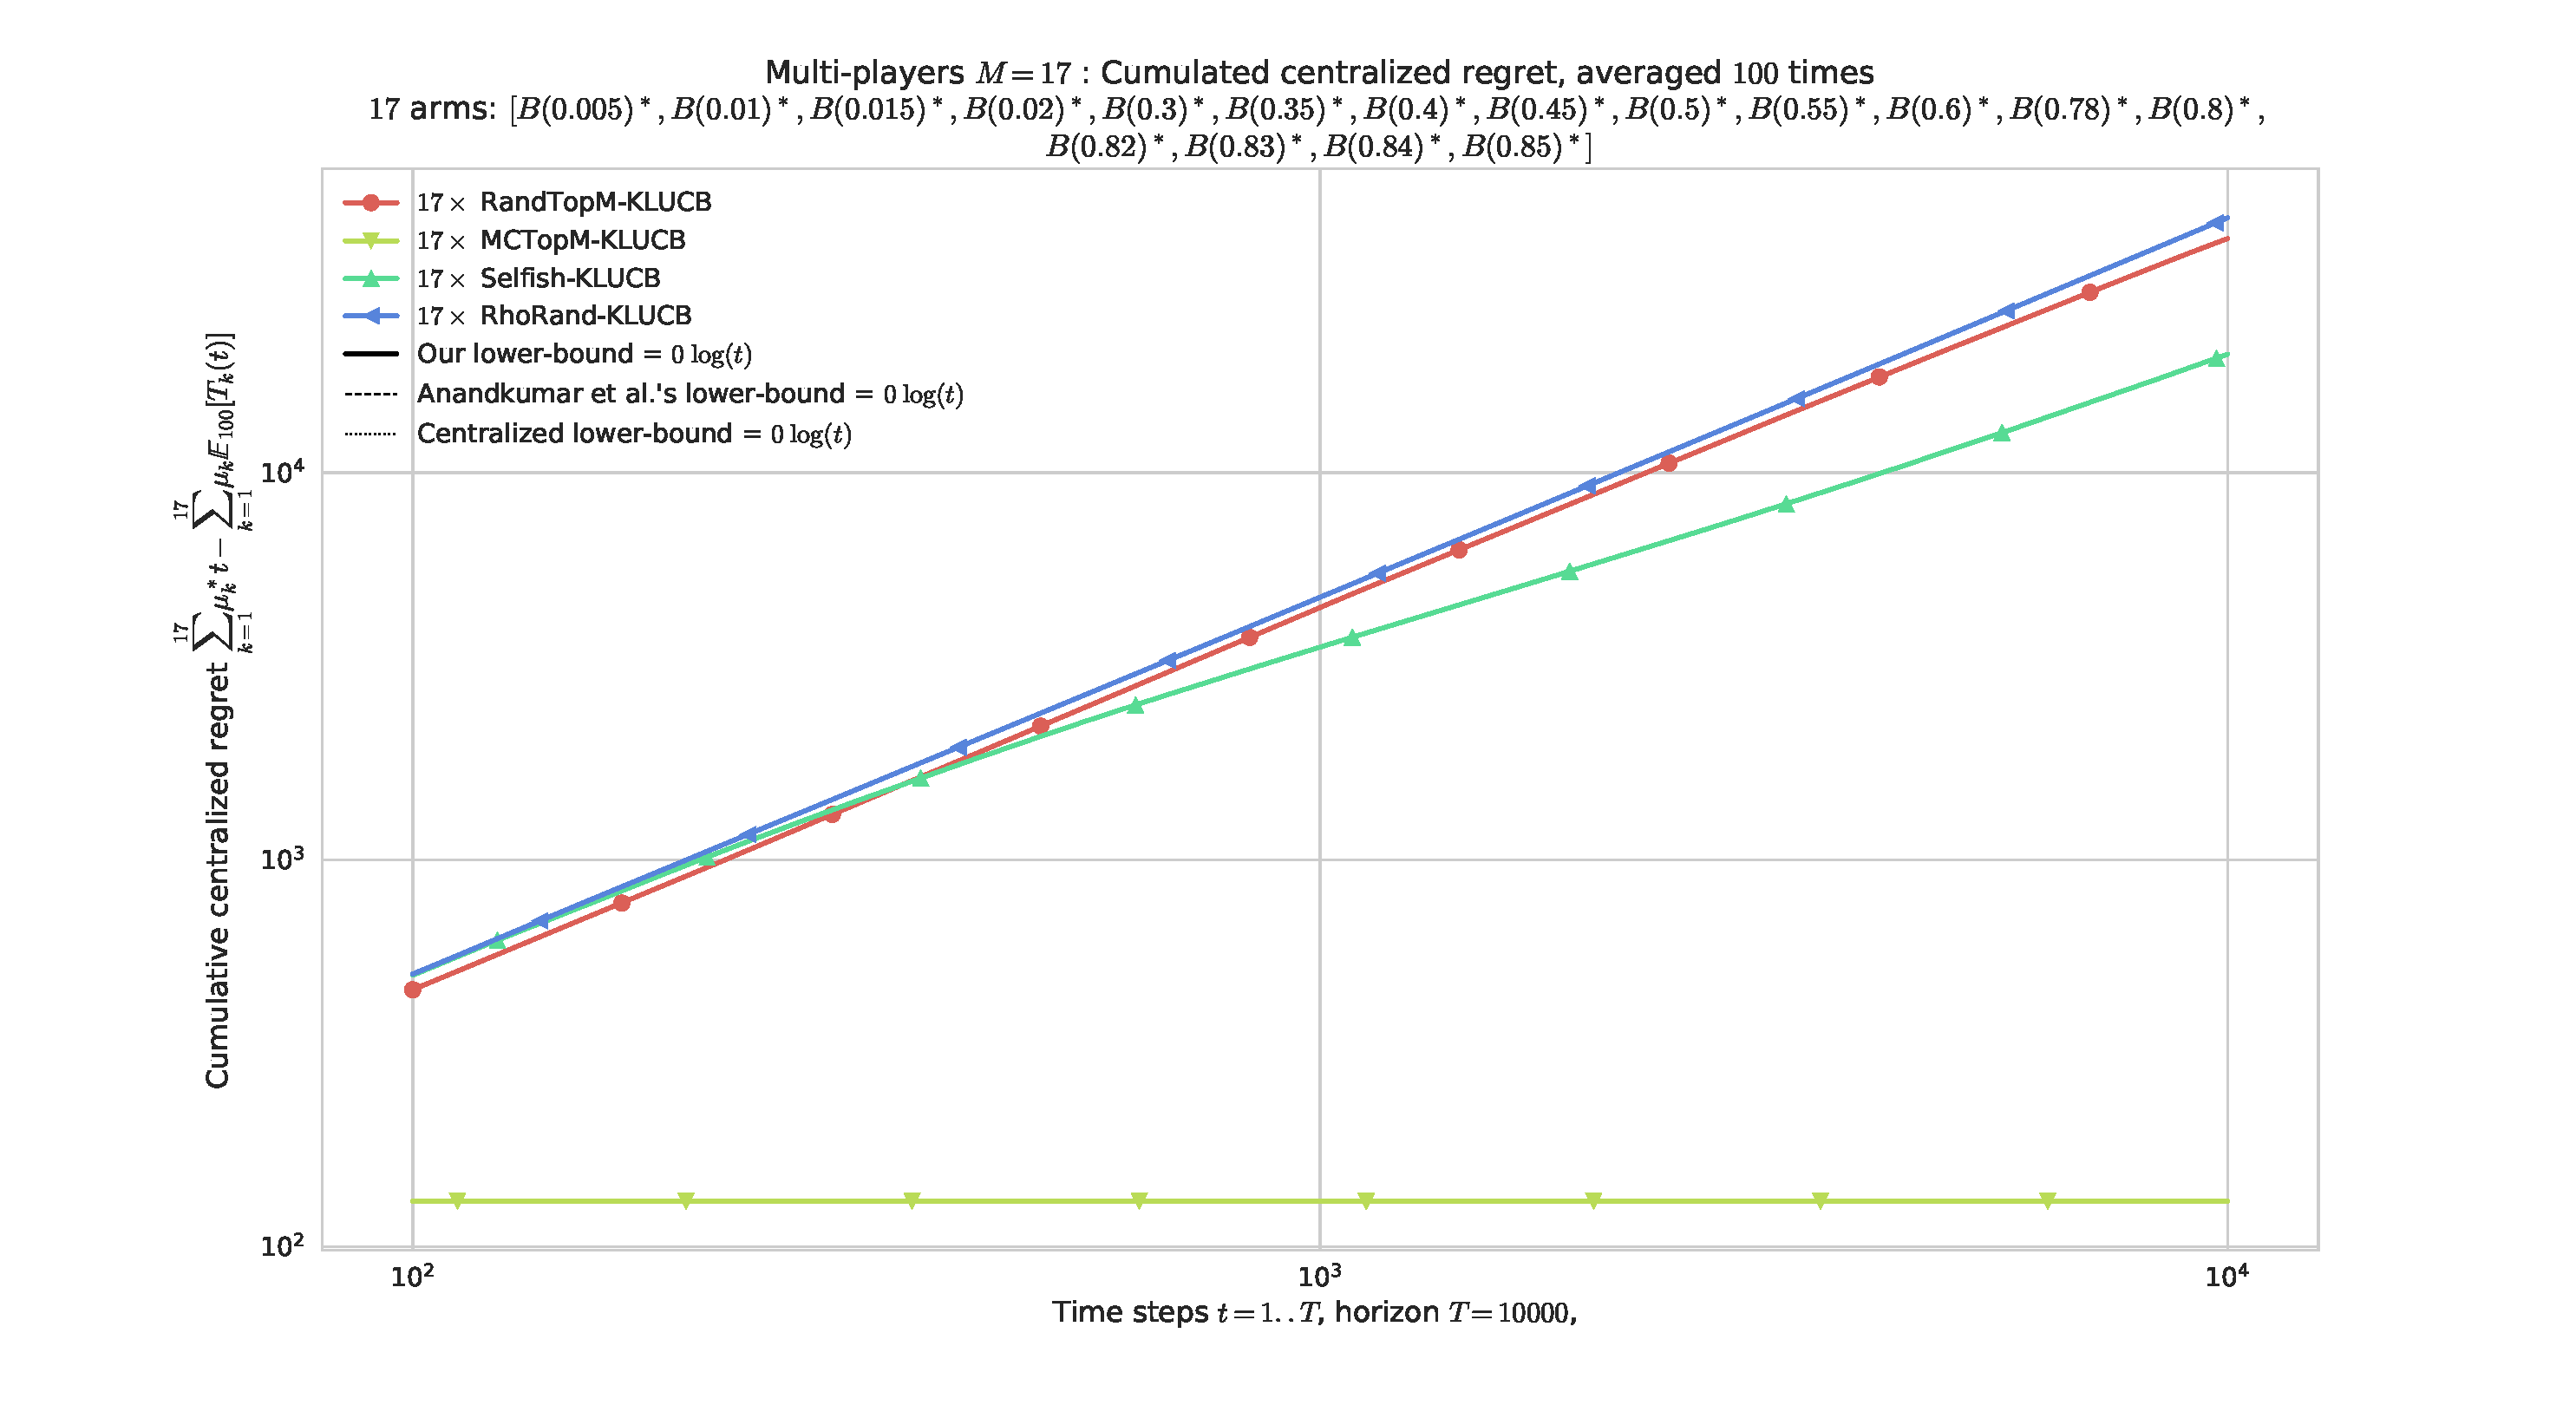
\includegraphics[width=1.00\textwidth]{MP__K17_M17_T10000_N100__4_algos/all_RegretCentralized_loglog____env1-1_8969236287861113966.pdf}
  % \end{subfigure}
  \caption[Regret for $M=6, 12, 17$ players for a ``difficult'' problem with $K=17$, and $T=5000$]{Regret (in log-log scale), for $M=6, 12, 17$ players for a ``difficult'' problem with $K=17$, and $T=5000$. The same observation as in Figure~\ref{fig:5:MP__K9_M2-6-9_T10000_N200__4_algos} can be made. \Selfish{} outperforms \MCTopM{} for $M=2$ here. Additionally, \MCTopM{} is the only algorithm to not fail dramatically when $M=K$ here.}
  \label{fig:5:MP__K17_M6-12-17_T10000_N100__4_algos}
\end{figure}



% -----------------------------------------------------------------
\section{Conclusion of our contributions}
\label{sec:5:conclusion}
% -----------------------------------------------------------------

To sum up, we presented three variants of Multi-Player Multi-Arm Bandits,
with different level of feedback being available to the decentralized players, under which we proposed efficient algorithms.
For the two easiest models --with sensing--, our theoretical contribution improves both the state-of-the-art upper and lower bounds on the regret. In the absence of sensing, we also provide some motivation for the practical use of the interesting \Selfish{} heuristic, a simple index policy based on hybrid indices that are directly taking  into account the collision information.

This work suggests several interesting further research directions.
First, one could want to investigate the notion of \emph{optimal algorithms} in the decentralized multi-player model with sensing information. So far we provided the first matching upper and lower bound on the expected number of sub-optimal arms selections, which suggests some form of (asymptotic) optimality. However, sub-optimal draws turn out not be the dominant terms in the regret, both in our upper bounds and in practice, thus an interesting future work is to identify some notion of \emph{minimal number of collisions}. Second, it remains an open question to know if a simple decentralized algorithm can be as efficient as \MCTopM{} without knowing $M$ in advance, or in dynamic settings (when $M$ can change in time). One could start by proposing variants of our algorithm that are inspired by the \rhoRandEst{} variant of \rhoRand{} proposed by \cite{Anandkumar11}.
Finally, one could want to strengthen the guarantees obtained in the absence of sensing, that is to know whether logarithmic regret is achievable and to have a better analysis of the \Selfish{} approach.  Indeed, in most cases, it performs comparably to \RandTopM{} even with limited feedback and without knowing the number of players $M$, which makes it a good candidate for applications to Internet of Things networks.


% -----------------------------------------------------------------


% \paragraph{Acknowledgments}
% Thanks to Odalric-Ambrym Maillard at Inria Lille for useful discussions, and thanks to Christophe Moy at University Rennes 1.

\paragraph{Reproducibility.}
The page \texttt{SMPyBandits.GitHub.io/MultiPlayers.html} explains how to reproduce the experiments used for this Chapter.

\begin{framed}
  \textcolor{red}{\textbf{FIXME}}
  Je ne sais pas trop comment inclure toutes ces figures ici, avant la dernière section où je parle des extensions de nos modèles.
  J'aimerai bien avoir quelques pages simplement remplies des figures, sans avoir le texte de Section~\ref{sec:5:literatureReviewOtherModels} qui commence au milieu...
  Une idée ?
\end{framed}



\newpage  % WARNING
% ----------------------------------------------------------------------------
% ----------------------------------------------------------------------------
\section{Literature review of many extensions of the models}
\label{sec:5:literatureReviewOtherModels}
% ----------------------------------------------------------------------------

Before concluding this chapter, we review many extensions to the three models presented above in Section~\ref{sec:5:model} that were introduced in recent literature.
%
We wanted to highlight that the community has been quite active on research on multi-player bandits in the last $10$ years, but especially active since last spring $2018$.
For instance, our article \cite{Besson2018ALT} was the first to propose the ``no sensing'' case, and it was studied by (at least) two independent group of researchers since its publication in April $2018$ \cite{BoursierPerchet18,LugosiMehrabian18}.
Another example is the model with different arm means among players, who was initially studied in \cite{Anandkumar10,Kalathil12} and then more recently in \cite{Bistritz18,KaufmannAbbas19}.
%
% FIXME écrit pas ça c'est inutile !
% By following actively the research on multi-player bandit models since the last three years, we believe to be able to give an exhaustive literature review, but it is of course possible that we missed an important research work. In this case, it is our mistake and not an intentional choice as we included all the different extensions of our models that we were aware of.

Many extensions of the simpler model of multi-player bandits have been considered.
The number of players $M$ can be fixed but initially unknown to the players, the sensing information can be absent (like the model \modeltrois{} presented above), there could be communications between players (happening at each time step or only occasionally), or $M$ could evolve over time to model the possibility of arrivals or departures of players (\ie, connexions and disconnections of devices in a wireless networks).
Also inspired by real-world wireless networks, the arm means may vary among players, for instance to model players located at different distance of the gateway, and we can also consider networks with some ``jammers'' whose purpose is not to communicate to the gateway in a collaborative way, like the $M$ devices, but to interfere with the communications of the $M$ devices.

Finally, we can also be interested by models where $M$ stays fixed, but the environment evolves, for instance with abrupt changes in the means of arms. This last model makes a good connexion between this chapter and the next one, and an exciting future work is to further study this model in order to tackle this kind of problems by merging our contributions for stationary multi-player bandits and for non-stationary single-player bandits.

% \TODOL{
%     Pour les extension présentées ici, je veux suivre la même organisation :

%     1. j'explique l'extension, et en quoi c'est difficile (= en quoi notre approche échoue si on fait rien de plus),

%     2. j'explique les travaux existants, et les résultats qu'ils obtiennent e.g. en terme de bornes de regret

%     3. si j'ai déjà le code pour, je peux montrer UNE simulation
% }


% ----------------------------------------------------------------------------
\subsection{Unknown (fixed) number of players}
\label{sub:5:unknownNumberOfPlayers}

In the model we presented above, we assumed the number of players $M$ to be fixed in time during the learning process.
Without removing this hypothesis (we study this case below in Section~\ref{sub:5:arrivalDepartures}), it is interesting to remark that we made no hypothesis on whether the players can known this value $M$ or not.
Our proposals, \RandTopM{} and \MCTopM, both assume to know $M$ beforehand, like it was done for their main inspiration, \RhoRand.


\paragraph{Performance of our proposals for a wrong value of $M$?}
\label{par:5:usingWrongValueofM}
%
We can start by asking whether the most efficient algorithm, \MCTopM-\klUCB, is still efficient if it uses a value $M'$ different than the real number of players $M$.
Even though we did not include numerical simulations for this case in Section~\ref{sec:5:experiments} above, we did some tests, which confirmed two disappointing results that were also proved analytically.
First, the three algorithms (\RhoRand, \RandTopM{} and \MCTopM) give linear regret if they are using a value $M'$ strictly smaller than $M$ (and if $\mu^*_{M-1} > \mu^*_M$), as players will converge to play about $T-\bigO{\log(T)}$ times the $M-1$ best arms, leading to at least one collision most of the time, and thus a linear regret.
Second, if the $M$ players falsely use a value $M' > M$, then there is also a certain (fixed) probability to achieve a linear regret. Indeed, imagine one player ($M=1$) running \MCTopM{} with the false knowledge of $M'=2$, and if it learned to accurately identify the set of the $2$ best arms, then the \MCTopM{} orthogonalization scheme can make it play the worst of the two arms, and as $M=1$ this player will never encounter any collision, thus playing this suboptimal arm for about $T-\bigO{\log(T)}$ times, also leading to linear regret.


\paragraph{Interpretation of the hypothesis of knowning $M$ for real-world networks.}
\label{par:5:knowingYourIDinMPBanditsGame}
%
One could criticize our approach if we study a wireless networks with no central coordination from the gateway,
in particular where the devices cannot be assigned to a channel or be assigned a unique ID by the gateway when they first log in the network.
Then in such networks, if one wants to apply an algorithm like \MCTopM-\klUCB,
the $M$ devices need to known their number $M$, and have to receive it from the gateway, as it is the only part of this example of network which knowns $M$.
It seems unrealistic to ask the gateway to send the fixed value $M$ to each device, and not a unique ID to each device, for instance $\mathrm{id}^j\in[K]$.

\TODOL{Expliquer pourquoi ce n'est pas très réaliste ? Le paragraphe ci dessous n'est pas très simple à comprendre, je peux faire mieux!}

If the $M$ players each have a unique ID, then a simple explore-then-commit algorithm running on top of a round-Robin phase can achieve order-optimal regret.
If the players know the time horizon $T$, then fix a confidence level $\delta$. For the first $T_0$ time steps, the $M$ players will use a simple round-Robin game, using their (unique) ID to stay orthogonal: player $j$ starts at arm $j$, then $j+1$, then cycle in $[K]$. They encounter no collision in these time steps, and then user $j$ targets the $j$-th best arm among the set of $M$-best arm.
If $T_0$ is large enough, all players have built the same estimate of the ranking of the arms (and not only correctly identified the set of $M$-best arms), with high probability (at least $\delta$), and thus they will also encounter no collision and no regret from after time $T_0$.
The mean regret of such approach is easily bounded by $R_T \leq M T_0 + (1 - \delta) (T - T_0)$, so by using $\delta = 1-1/T$, $R_T = \bigO{T_0}$.
By calibrating $T_0$ based on $\delta$ (which needs prior knowledge of $T$) and the minimal gap $\Delta$ between \Mbest{} and \Mworst, one can show, using similar arguments as used by \cite{Rosenski16} for the Musical Chair policy, that with large probability a constant regret is obtained. A logarithmic regret can be obtained from the same bound, proving the order-optimality of this simple approach, if we assume that user $j$ knows it is user number $j$.
%
Without giving more details, we let the interested refer to what is is explained for the algorithms presented in \cite{DarakHanawal18,JoshiKumar2018,KumarDarak2019}.
%
These works assume a prior knowledge of $\Delta$, or other measures of the difficulty of the problem, and as such we do not find them comparable with the approach chosen here.


\paragraph{Two ideas to estimate $M$.}

Some works studied the same model as our model \modeldeux{} ``with sensing'', under the hypothesis that players do not know in the value of $M$.
As illustrated above, if we consider algorithms building on the same ideas as \RhoRand{} or \MCTopM, it seems mandatory to first build an estimate of the value of $M$ then run the initial algorithm that assumed a perfect knowledge of $M$.
Two possible directions exist to estimate $M$ on the fly.

The first idea comes from \cite{Anandkumar11}, and the intuition behind it is quite simple, even if the mathematical derivations are not.
All players will build an estimate $\hat{M}^j(t)$ of the number of player, that start by $\hat{M}^j(0)=1$. As soon as one collision is observed, a player knows that $M\geq2$, so $\hat{M}^j(t+1) = 2$.
Then, based on probabilistic computations on the expected number of collisions if there were $m$ players, all following the same strategy (\eg, \RhoRand{} in the case of ), and because the formula is simple to compute for different $m$, the authors proposed a statistical test of the hypothesis $M \leq \hat{M}^j(t)$ against $M > \hat{M}^j(t)$ which is expressed as a simple comparison of the current number of collisions (since last update of $\hat{M}^j(t)$) against a threshold.
If a player observed ``too many'' collisions (that are unlikely to be caused by only $\hat{M}^j(t) - 1$ other players), then she increases her current estimate $\hat{M}^j(t+1) = \hat{M}^j(t) + 1$.

The second idea comes from \cite{Rosenski16}, and suppose to know beforehand both the horizon $T$ and a certain measure of the difficulty of the problem (\ie, a lower bound on the minimal gap between two means).
If all the $M$ players start to play for a long enough time $T_0$ uniformly at random among all the $K$ arms, then the (expected) number of collisions observed $\E[\cC^j_{T_0}]$ by any player $j$ is a (relatively simple) function of $M$. By knowing $K$ and $T_0$ and if all players use the same mechanism, then they can invert the formula to obtain the most likely estimate of $M$ which explained the observations of $\cC^j_{T_0}$ collisions.
This second approach works empirically very fine, but it requires a fine tuning of the stopping time $T_0$.
Rosenski et al. studies the performance of their algorithm with high-probability bounds \cite{Rosenski16}, and the tuning of $T_0$ they propose depends on prior knowledge on the problem.
%
For this reason, we are not fond of this approach, as this hypothesis is quite unrealistic if one wants to apply this kind of algorithms for real-world wireless networks.
We note that all the following works assume some sort of prior knowledge on the difficulty of the problem:
\cite{kumar2017channel,KumarYadav2018,SawantKumar2018,JoshiKumar2018,DarakHanawal18,KumarDarak2019,Tibrewal2019}.


\paragraph{Extension of our proposals to learn the value of $M$.}

Similarly to what was proposed for the \rhoRandEst{} algorithm in \cite{Anandkumar11}, we could have worked on proposing and analyzing an extension of our proposals that could efficiently learn the value of $M$ the number of player.
We implemented this \rhoRandEst{} policy in our library SMPyBandits \cite{SMPyBandits}, as well as this mechanism for \RandTopM{} and \MCTopM.
Building from the theoretical analysis given for \rhoRandEst{} in \cite{Anandkumar11}, and the analysis of \MCTopM-\klUCB, we believe it is possible to show that the aforementioned extension also achieves sub-linear regret without requiring players to know $M$ in the beginning of the bandit game.
More precisely, we believe that \MCTopM-\klUCB{} can still give order-optimal logarithmic regret if $M$ players use it, and this extension of Theorem~\ref{thm:5:LogarithmicRegret_MCTopMklUCB} is not included due to space constraints.
Writing its proof and performing more simulations are left as possible future work.

\paragraph{Simulations.}

We consider a bandit problem with $K=9$ arms, of means $0.1,\dots,0.9$, and three different cases of $M=3,6,9$ players, for $100$ independent repetitions and an horizon of $T=10000$.
As before, we include the centralized multiple-play \klUCB{} as an unachievably efficient baseline, the \Selfish-\klUCB{} algorithm as an heuristic which does not require the know $M$.
Then we compare the \RhoRand, \RandTopM{} and \MCTopM{} algorithms, using \klUCB, which know $M$ beforehand, with their extensions implementing the same algorithm as \rhoRandEst, to estimate $M$ on the fly.

% \TODOL{Include a simulation to show the behavior of \rhoRand{} vs \rhoRandEst, and \RandTopM{} and \MCTopM{} with prior knowledge of $M$ vs the ``estimate'' versions.}
% Je dois refaire ces simulations, les chiffres ici sont avec $T=1000$ et $N=4$ répétitions (juste faites vite fait dans le train, je dois les lancer sur la machine du bureau).
% for M in 3 6 9; do DEBUG=False SAVEALL=True NOPLOTS=True M=$M K=9 N_JOBS=-1 N=100 T=10000 make moremultiplayers; read; done



\begin{table}[ht]
\begin{small}  % WARNING
    \centering
    \begin{tabular}{cc|ccc}
    \textbf{Algorithms} & \textbf{Hyp. on $M$} & $M=3$ players & $M=6$ players & $M=9$ players \\
        \hline
        Centralized multiple-play
        & Known $M$ & $\mathbf{92 \pm 20}$ & $\mathbf{70 \pm 16}$ & $\mathbf{0}$ \\
        \hline
        \Selfish
        & Don't need $M$ & $250 \pm 34$ & $735 \pm 85$ & $3010 \pm 472$ \\
        \hline
        \multirow{2}{*}{\RhoRand}
        & Known $M$ & $417 \pm 103$ & $2481 \pm 449$ & $6639 \pm 1035$ \\
        & \textcolor{red}{Estimate $M$} & \textcolor{red}{$1422 \pm 1051$} & \textcolor{red}{$9030 \pm 1922$} & \textcolor{red}{$7264 \pm 1009 $} \\
        \hline
        \multirow{2}{*}{\RandTopM}
        & Known $M$ & $268 \pm 45$ & $941 \pm 217$ & $437 \pm 367$ \\
        & \textcolor{red}{Estimate $M$} & \textcolor{red}{$688 \pm 614$} & \textcolor{red}{$4256 \pm 2701$} & \textcolor{red}{$1155 \pm 544$} \\
        \hline
        \multirow{2}{*}{\MCTopM}
        & Known $M$ & $244 \pm 39$ & $401 \pm 55$ & $44 \pm 13$ \\
        & \textcolor{red}{Estimate $M$} & \textcolor{red}{$563 \pm 546$} & \textcolor{red}{$1560 \pm 1293$} & \textcolor{red}{$618 \pm 29$} \\
        \hline
    \end{tabular}
    \caption{Mean regret $\pm$ $1$ std-dev, for different algorithms on the same problem with $M=3,6,9$, comparing algorithms which knows $M$ against algorithms which estimate $M$ on the fly. All use \klUCB.}
    \label{table:5:meanRegretSimulationsEstimatingM}
\end{small}  % WARNING
\end{table}

One can observe in Table~\ref{table:5:meanRegretSimulationsEstimatingM} the empirical performances of different algorithms in an example problem, in each case of low, medium and maximum number of players ($M=3,6,9$ for $K=9$ arms).
The three algorithms \RhoRand, \RandTopM{} and \MCTopM{} all suffer from similar increase on their regret when they have to estimate $M$ on the fly (written ``Estimate $M$'' in red, in Table~\ref{table:5:meanRegretSimulationsEstimatingM}). Our proposals are still much more efficient than \RhoRand{} when using the procedure to estimate $M$ described from \cite{Anandkumar11}.
For the two non-extreme cases ($M=3,6$), the performance drop when having to estimate $M$ is quite large,
% (on the three algorithms and two cases, about $\times 3.4$),
and consistent on the different algorithms.
The extreme case of $M=K$ players is of highest interest, as \MCTopM{} achieves a very small regret (proved to be $\cO(1)$ as it is just the expected time of the orthogonalization process), while the same algorithm with unknown $M$ suffers from a much larger regret.
In this extreme case, \RhoRand{} and its extension both perform very closely, as expected, and much worse than \MCTopM.
%
Additional simulations, for increasing time horizons $T$, confirmed the expected order-optimal regret of this extension of \MCTopM-\klUCB.


% ----------------------------------------------------------------------------
\subsection{Arrival and departures of players: the ``dynamic setting''}
\label{sub:5:arrivalDepartures}

As reminded above, the model assumes the number of players $M$ remain fixed during all the bandit game.
However, in real-world wireless networks, when players model communicating devices connected to a single gateway, devices can arrive or leave the network at any time.
The existing previous work on multi-player bandit models are all motivated by possible applications to wireless networks, but most of them assume $M$ to be fixed.
The first work studying the relaxation of this hypothesis is \cite{Rosenski16}, where this case is called the ``dynamic setting''.
If the arrival or departures of players is not random, but determined in advance while still being unknown to any player, the natural notion of regret is the following, where the expectancy $\E[\bullet]$ is capturing the randomness in the sensing information, as well as in the players' decisions (\ie, collisions):
\begin{equation}\label{eq:5:defRegretDynamicSetting}
    R_T^{\text{dyn}} = \sum_{t=1}^T \sum_{k=1}^{M(t)} \mu^*_{k} - \E\Bigl[ \sum_{t=1}^T \sum_{j=1}^{M(t)} r^j(t) \Bigr].
\end{equation}

In \cite{Rosenski16}, the authors explain that if the model allows arrival or departures of players at \emph{any time step}, then the game is much harder, and sub-linear regret is most likely un-achievable, if we consider the natural extension of the definition of regret as in our model presented in Section~\ref{sec:5:model} above.
However, this negative results depends on how arrival of players are modeled:
if an arriving player has no prior memory of the previous observations, \ie, if it model a new device, then if there is no restriction on the number or frequency of arrival or departures, we can most likely prove that sub-linear regret is not achievable in general.
A simple but extreme example shows that regret has to be linear for any bandit strategy (in the observation model with sensing).
Consider $K=2$ Bernoulli-distributed arms of means $\mu_1=\mu_2=1/2$, and one player is always active and play any bandit strategy (\eg, \MCTopM-\klUCB).
Every time step, another player is either arriving, without any knowledge of the problem (\eg, it is a fresh and new IoT device). Then no matter the strategy of these news players, even if they all play \MCTopM-\klUCB{} for instance, if they play a uniformly-efficient strategy there is a non-zero probability that player $1$ suffer from a collision at each time step, thus resulting in linear centralized system regret.

In \cite{Rosenski16}, it is assumed that the players all know a lower-bound $L$ on the length of all the intervals during which arrival or departures of players are allowed.
A naive idea, if $L$ is large enough, is simply to restart the underlying algorithm every $L$ time steps, in order to directly benefit from the theoretical guarantees of the ``static setting'' (where $M$ stays constant).
However, this idea yields a large regret if the length of ``static'' intervals $L$ is too small.
Applied to the \MusicalChair{} algorithm, the authors in \cite{Rosenski16} call this basic extension Dynamic \MusicalChair
Under the simple hypothesis that the overall number of players entering and leaving the game is sub-linear in $T$ (\ie, a $\smallO{T}$), they analyze the regret of Dynamic \MusicalChair{} and prove it is also sub-linear (see Theorem~2 in Section~3.4).
%
Under the same hypothesis, and if the lower-bound $L$ is known before-hand and is large enough, then we could also apply the same idea as from \cite{Rosenski16} to our approach. We believe that we could easily prove that a sub-linear regret is achievable, if all players run \MCTopM-\klUCB{} (and if currently active players restart their memory of the past observations every $L$ time steps).
As the regret guarantees are stronger (\ie, smaller regret upper-bound) for \MCTopM{} than \MusicalChair, we also believe that in this ``slowly varying'' dynamic setting, applying the idea of Dynamic \MusicalChair{} from \cite{Rosenski16} to \MCTopM{} would also give a small regret upper-bound.

After being introduced in \cite{Rosenski16}, some more recent works studied the case of arrival or departures of players, usually referred to as ``dynamic setting'' or ``dynamic case''.
For instance, \cite{BoursierPerchet18} studies in Section~4 the first algorithm proposed for the dynamic case under the no-sensing model.
They study the same notion of regret as the one proposed in \cite{Rosenski16} and given above in \eqref{eq:5:defRegretDynamicSetting}, see Equation $(10)$ in Section~4.2.1.
With the assumption of a non-decreasing number of players, \ie, if only arrivals of players are considered,
they prove a regret upper-bound of the \textsc{Dyn-MMAB} algorithm in Theorem~3 .
% Denote $M(t)$ the number of players at each time $t$, then they propose to study $R_T$ defined as
% \[ R_T = \sum_{t=1}^T \sum_{k=1}^{M(t)} \mu_^*{k} - \sum_{t=1}^T \sum_{j=1}^{M(t)} r^j(t). \]
If all arriving players are using their \textsc{Dyn-MMAB} algorithm, the ``dynamic'' regret is bounded by $\bigO{M^2 K \log(T) / \mu^*_{M}}$, if $M=M(T)$ is the total number of players involved in the problem.

% \TODOL{Present the model, quote the main papers, explain the difficulty and how XXX algorithm solves it!}


% \cite{KumarYadav2018}

% Distributed Learning and Stable Orthogonalization in Ad-Hoc Networks with Heterogeneous Channels
% Sumit J Darak, Manjesh K. Hanawal
% https://arxiv.org/pdf/1812.11651
% \cite{DarakHanawal18}


% ----------------------------------------------------------------------------
\subsection{Without sensing information}
\label{sub:5:withoutSensing}

We presented in Section~\ref{sec:5:model} the model \modeltrois, without sensing information. Players can only observe $Y_k(t)$, the product of the \iid{} random sensing information from arm $k$ and of the no-collision indicator.
This model seems harder than the model with sensing information, and even though the proposal \Selfish{} works fine in simulations (in terms of average regret), we proved that it can yield linear regret.
In our paper \cite{Besson2018ALT} as well as the previous sections, it was left as a future work to know if an algorithm can achieve sub-linear regret in this harder model without sensing information.

Inspired by \cite{Besson2018ALT},
Boursier and Perchet studied this question in the summer $2018$ following its publication \cite{BoursierPerchet18}.
Their answer is that the model without sensing information is essentially not harder than the model with sensing information.
%
Similarly, Lugosi and Mehrabian studied the same problem \cite{LugosiMehrabian18}.
In both works, the authors detail algorithms that give in both cases a logarithmic regret if $M \leq K$ players all independently implement the proposed algorithm.


\paragraph{The ``communication trick''.}
%
% \TODOL{Write about half a page on the article \cite{BoursierPerchet18}.}

The recent work \cite{BoursierPerchet18} proposed an idea they called the ``communication trick''.
It essentially allow any player to send one bit to all the others, at some pre-agreed time steps, with no modification on the model.
Thanks to this ``communication trick'', recent research efforts have been more focus on studying the basic model --without explicit communications between players--, while proposing algorithms that can rely on some communication between players.
This trick essentially use the fact that the players share a synchronized time, thus they can use a collision as a way to directly exchange one bit of information between two players.
This process is slow and not efficient, as all but two players must do nothing when player $i$ is sending a bit to player $j$, but it does build a communication protocol in the model without explicit communication between players.
This ``communication trick'' is used for instance in \cite{KaufmannAbbas19}.
We let the interested reader refer to these last two works \cite{BoursierPerchet18,KaufmannAbbas19} as they are both solid, and well explained.


\paragraph{Estimating collisions through uniform exploration.}
%
\cite{LugosiMehrabian18} gives a first algorithm with expected regret of $\bigO{M K \log(T) / \Delta^2}$, if $\Delta = \mu^*_{M} - \mu^*_{M+1} \neq 0$, achieving a better dependency regarding $M$ when compared to our result (our bound is $\bigO{M^3}$) but at the cost of (much) larger constants hidden in the $\cO$ notation, and a non-fully explicit algorithms which usually obtain bad (or worse) empirical performance.
Then they study an interesting extension that works also if $\Delta = 0$ or if $\Delta$ is so close than the bound in $1/\Delta^2$ becomes useless for ``small horizons''. This behavior is well known for classical bandits, where bounds of the form $\log(T)/\Delta^2$ become worse than a linear regret $T$ if $\Delta$ is very small (\ie, $\Delta\ll \sqrt{\log(T)/T}$).
For this extension, their proposed algorithm is proved to achieve $\bigO{K^2 M (\log(T))^2 / \mu + K M \min(\sqrt{T \log(T)}, \log(T)/\Delta')}$ regret, if $\mu$ is a lower-bound on $\mu^*_{M}$ and $\Delta' = \max(\Delta, \min\{|\mu^*_M-\mu^*_i| : \mu^*_M > \mu^*_i \})$ (that both have to be known beforehand by the algorithm).
%
The proposed algorithms in \cite{LugosiMehrabian18} are all based on the Musical Chair algorithm from \cite{Rosenski16}, and the curious reader should read for instance their Algorithm~2 (page 15) for more details.

The results presented in \cite{LugosiMehrabian18} are based on some hypotheses, for instance the tuning they propose for the length $g$ of the uniform exploration phase in the beginning of their ``Musical Chair''-like algorithm is based on a prior knowledge of the horizon $T$.
In Section~4 they explain how to relax the assumptions of their results.
For the same example, the ``doubling trick'' technique can be used to obtain a regret upper bound for an algorithm unaware of the value of $T$, within a constant multiplicative factor of the upper bound given for the algorithm aware of $T$ (Section~4.1). Because the regret bound is of the form $\bigO{\sqrt{T} \log(T)}$, a simple ``doubling trick'' of increasing horizons of lengths $T_i = 2^i$ works well, as proposed in \cite{CesaLugosi06} and as studied in depth in our article \cite{Besson2018DoublingTricks}, and quickly presented in Appendix~\ref{app:2:DoublingTricks}.
%
They also study in Section~4.3 an extension of the model for the case with more players than arms, but we do not give more details on this aspect. Their definition of a centralized regret for this case is an interesting and natural generalization of the definition, and they also proposed an algorithm achieving $\bigO{M K \log(T) \exp(4M/K) / \Delta^2}$ regret in this case.
Finally, they also proposed in Section~4.4 an extension of their algorithm to estimate the number of players $M$, which is analyzed as for the Musical Chair algorithm in \cite{Rosenski16}, and also achieve logarithmic regret.
Note that it is significantly harder to estimate $M$ without collision information, and Algorithm~3 in page 24 is quite complex.
We did not implement it, and it would be interesting to run some numerical simulations in order to validate it empirically.


\paragraph{About \Selfish-\UCB{} inefficiency.}
%
It is also proved in Appendix~A of \cite{BoursierPerchet18} that \Selfish-\UCB{} has a linear regret, in the theoretical case, with a very neat argument from number theory (using Lindemann-Weierstrass theorem). As we conjectured, there is a gap between the theoretical result and its practical consequence, as the Theorem~4 they gave is only valid for real-valued number, and not for hardware-represented floating point number.
Their proof is supporting what we illustrated in Figure~4 in \cite{Besson2018ALT}.
Their argument is essentially to prove that for \Selfish-powered players using the simple \UCB-indexes, with a probability $p$ at time $t$ (both independent from $T$), two players might have the same number of pulls and the same observed rewards for each arm. In that case, the two players would pull the exact same arms and thus collide for a long time, until they reach a ``tie breaking point'' where they could choose different arms thanks to a random tie breaking rule (\eg, if two values of their \UCB{} indexes are the same, the $\argmax$ is a uniform random choice among the two arms).
They prove that it is unlikely to encounter any of these ``tie breaking points'', in theory if the \UCB{} indexes are real-valued number (that can be rational or irrational).


\paragraph{Additionnal numerical simulations.}

To illustrate the difficulty of the ``no sensing'' case, we illustrate here the performances of different algorithms designed specifically for this setting.
As above, we consider a bandit problem with $K=9$ arms, of means $0.1,\dots,0.9$, and three different cases of $M=3,6,9$ players, for $100$ independent repetitions and an horizon of $T=10000$.
We include the \Selfish-\klUCB{} algorithm as an heuristic, as well as the Improved \MusicalChair{} algorithm from \cite{LugosiMehrabian18} and \textsc{Sic-MMAB} from \cite{BoursierPerchet18}.
The centralized multiple-play \klUCB{} is included as an unrealistic efficient baseline, but it is interesting to also add it here, as it does not use the sensing information but only the joint information (the reward) $r^j(t)$, as it directly affects the player in an orthogonal configuration and thus never encounters any collision (thus $r^j(t)=Y_{t,A^j(t)}$ for each $j,t$).
%
For the two other algorithms, we use the parameters advised in all papers: for \textsc{Sic-MMAB}, we used $T_0 = \lceil K \log(T) \rceil$ as advised by the authors.
For Improved-MC, we used $c=1$ which gives $g=235$, whereas in the paper the authors use $c=128$ for their analysis. We found empirically no difference when using different values of the constant $c$ or $g$, and unfortunately the regret of Improved-MC was always found to be linear\footnote{For instance Improved-MC obtained a mean regret $12150$ for $T=10000$, for $M=3,K=9$, but seeing one value for one horizon does not mean anything, however we also experimented with larger values of $T$ and found a same linear behavior.}.

% for T in 10000; do for K in 9; do for N in 4 100; do for M in 3 6 9; do DEBUG=False N_JOBS=4 N=$N K=$K M=$M T=$T make --noFreeSMS moremulti && cp logs/main_multiplayers_more_py3_log.txt logs/main_multiplayers_more_py3_log__K${K}_N${N}_M${M}_T${T}_$(date +"%d-%m-%Y_%H-%M-%S").txt && FreeSMS.py "Done for simulations for $K arms, $M players, T=$T N=$N and lots algorithms for experiments for Chapter 5 of my PhD. Love from Rennes."; done; done; done; done

We give in Table~\ref{table:5:meanRegretSimulationsNoSensing}, we give the mean regret obtained for these different algorithms, and we observe a drastic difference between the unrealistic centralized algorithm, which achieves a very small regret, the heuristic \Selfish-\klUCB{} which achieve small mean regret (but is small to fail in theory and in some instances), and the two other algorithms.
We were unable to find any bug in our implementation of Improved \MusicalChair{} from \cite{LugosiMehrabian18} and all the different tuning of $c$ (or $g$) explored gave the same disappointing result (linear regret).
The \textsc{Sic-MMAB} algorithm performs better than the \Selfish{} heuristic for the extreme case of $M=K$, but its large regret in this case shows that the orthogonalization protocol developed by \cite{BoursierPerchet18} is not fast to converge (for illustration, for the same problem for $M=K=9$ for the ``sensing'' case, \MCTopM-\klUCB{} achieves a mean regret of about $40$, two orders of magnitude smaller!).
%
Further empirical evaluation would be needed to fully understand the situation, and a first future work would be to either fix our implementation of the algorithm proposed by \cite{LugosiMehrabian18} or propose an efficient modification, and illustrate in some problems that it can indeed achieve sub-linear regret (maybe it does but only for large horizons, even if we did try larger values of $T$ like up-to $T=200000$).

\begin{table}[ht]
    % \begin{footnotesize}
    \centering
    \begin{tabular}{c|ccc}
    \textbf{Algorithms} $\;$ \textbackslash $\;$ \textbf{Number of players} & $M=3$ & $M=6$ & $M=9$ \\
        \hline
        Centralized Multiple play \klUCB{} & $\mathbf{91 \pm 21}$ & $\mathbf{70 \pm 16}$ & $\mathbf{0 \pm 0}$ \\
        \Selfish-\klUCB{} & $249 \pm 35$ & $728 \pm 94$ & $2953 \pm 501$ \\
        \hline
        \textsc{Sic-MMAB} & $1705 \pm 340$ & $3915 \pm 300$ & $1713 \pm 52$ \\
        Improved \MusicalChair{} & $\textcolor{red}{12149 \pm 60}$ & $\textcolor{red}{22341 \pm 77}$ & $\textcolor{red}{27462 \pm 85}$ \\
        \hline
    \end{tabular}
    % \caption{Mean regret $\pm$ $1$ std-dev, for different algorithms on the same problem with $M=3,6,9$, for the ``no sensing'' case.}
    \caption{Comparison for different algorithms on the same problem with $M=3,6,9$ players, for the ``no sensing'' case. We give the mean regret $\pm$ $1$ std-dev, and more work is needed on our implementation on Improved \MusicalChair. The results on \textsc{Sic-MMAB} appear to confirm the numerical experiments in the paper \cite{BoursierPerchet18}.}
    \label{table:5:meanRegretSimulationsNoSensing}
% \end{footnotesize}
\end{table}

% % M=3
% SIC-MMAB(kl-UCB, $T_0=226$) : 1705 ± 340
% TSN($T_{RH} = 140, T_{SH} = 1.53e+04$) : 9001 ± 2
% Selfish-kl-UCB : 249 ± 35
% CentralizedMultiplePlay(kl-UCB) : 91 ± 21
% MusicalChair($T_0=1000$) : 1410 ± 641
% MusicalChair($T_0=450$) : 1268 ± 1110
% MusicalChair($T_0=900$) : 1355 ± 681
% MusicalChair($T_0=1350$) : 1791 ± 561
% MusicalChair($T_0=95117$) : 12145 ± 59
% MusicalChair($T_0=118764$) : 12142 ± 59
% MusicalChair($T_0=220257$) : 12146 ± 59
% MCNoSensing($M=3$, $T=10000$, $c=1$, $g=235$) : 12149 ± 60
% MCNoSensing($M=3$, $T=10000$, $c=10$, $g=2.35e+03$) : 12148 ± 66
% MCNoSensing($M=3$, $T=10000$, $c=128$, $g=3.01e+04$) : 12149 ± 56

% % M=6

% SIC-MMAB(kl-UCB, $T_0=226$) : 3915 ± 300
% TSN($T_{RH} = 140, T_{SH} = 1.53e+04$) : 9008 ± 5
% Selfish-kl-UCB'  : 728 ± 94
% CentralizedMultiplePlay(kl-UCB)' : 70 ± 16
% MusicalChair($T_0=1000$) : 3130 ± 1583
% MusicalChair($T_0=450$) : 2690 ± 2473
% MusicalChair($T_0=900$) : 3015 ± 1839
% MusicalChair($T_0=1350$) : 3403 ± 1202
% MusicalChair($T_0=95117$) : 22363 ± 89
% MusicalChair($T_0=118764$) : 22352 ± 74
% MusicalChair($T_0=220257$) : 22352 ± 75
% MCNoSensing($M=6$, $T=10000$, $c=1$, $g=235$) : 22341 ± 77
% MCNoSensing($M=6$, $T=10000$, $c=10$, $g=2.35e+03$) : 22365 ± 80
% MCNoSensing($M=6$, $T=10000$, $c=128$, $g=3.01e+04$) : 22349 ± 84

% % M=9
% SIC-MMAB(kl-UCB, $T_0=226$) : 1713 ± 52
% TSN($T_{RH} = 140, T_{SH} = 1.53e+04$) : 39 ± 18
% Selfish-kl-UCB : 2953 ± 501
% CentralizedMultiplePlay(kl-UCB) : 0 ± 0
% MusicalChair($T_0=1000$) : 2775 ± 27
% MusicalChair($T_0=450$) : 1455 ± 1059
% MusicalChair($T_0=900$) : 2506 ± 30
% MusicalChair($T_0=1350$) : 3737 ± 36
% MusicalChair($T_0=95117$) : 27466 ± 90
% MusicalChair($T_0=118764$) : 27480 ± 80
% MusicalChair($T_0=220257$) : 27467 ± 95
% MCNoSensing($M=9$, $T=10000$, $c=1$, $g=235$) : 27462 ± 85
% MCNoSensing($M=9$, $T=10000$, $c=10$, $g=2.35e+03$) : 27463 ± 101
% MCNoSensing($M=9$, $T=10000$, $c=128$, $g=3.01e+04$) : 27462 ± 76


% ----------------------------------------------------------------------------
\subsection{With communication or coordination between players}
\label{sub:5:withCommunicationOrCoordination}

In all the models of IoT networks considered in this thesis, we assume that \emph{the different IoT devices cannot communicate with each other}, and can only communicate with a unique gateway.
Of course, this hypothesis can be removed, and in practice in some families of wireless networks, communication between devices are possible.
Note that this extension is not considering a graph of distributed agents all playing cooperatively to solve a unique bandit game, like it is studied in the ``\emph{graph bandit}'' problem.
What we are interested here is an extension of the model where players can send some bits to one or all the other players, at every time steps or some time steps.

Clearly, the problem is easier by allowing communication, and it is quite immediate to see that the communication capacity between players must be limited otherwise the problem is already known and solved.
Indeed, imagine that at each time step $t$, all the $M$ players could share an unbounded number of bits with the other players, at no cost, even if this hypothesis is clearly unrealistic for wireless networks.
Then they can share all their observations, and they can all run the same multiple-plays MAB algorithm \cite{Anantharam87a}, like for instance the extension of Thompson sampling for multiple-plays studied in \cite{Komiyama15}, or extensions of \KLUCB{} from \cite{Luedtke16}.
In this setting, a logarithmic regret is obtained easily, and the regret upper-bound of the two aforementioned algorithms asymptotically achieve the lower-bound from \cite{Anantharam87a}.

An interesting extension is thus to limit the communication between players, either to a small number of bits, or just one bit, at every or only some time steps.
We identified that the state-of-the-art on this direction of research consists in the two very recent works
% published in April 2019, while I was finishing this chapter:
\cite{tao2019collaborative} and \cite{wang2019distributed}.
Distributed pure exploration is studied in \cite{tao2019collaborative}, where the proposed new lower bounds for the regret of any algorithm for the distributed best arm identification problem, under the fixed time or fixed confidence settings.
The also propose effective algorithms that asymptotically match their lower-bounds (up-to logarithmic factors, in some cases).
The second work studies distributed learning for (not necessarily stochastic) multi-armed bandits as well as linear bandits \cite{tao2019collaborative}.
For a distributed $K$-armed bandit with $M$ agents, they developed two protocols achieving near-optimal regret $\cO(\sqrt{M K T \log(T)})$,
and requiring little communication cost,
one is independent of the time horizon $T$ and use $\cO(M \log(T))$ communications,
and the other is independent of the number of arms $K$ and use $\cO(M K \log(M))$ communications.
Their model and algorithms fit in the distributed, decentralized framework we advertise in all this thesis, and this last work is very interesting.

Additionally, after the recent work \cite{BoursierPerchet18} introduced the ``communication trick'',
some recent research efforts have been more focus on studying the basic model --without explicit communications between players--, while proposing algorithms that can rely on some communication between players.
This ``communication trick'' is used for instance in \cite{KaufmannAbbas19}.
Due to space constraint, we let the interested reader refer to these last two works \cite{BoursierPerchet18,KaufmannAbbas19} as they are both solid, and well explained.

Another line of research is to consider models that are closer to realistic wireless communication networks, as it is done in \cite{Avner16,AvnerMannor18}.
Explaining in details their model and proposed solutions would be quite lengthy, and we rather prefer to let the interested reader refer to the later work \cite{AvnerMannor18}.
We sum-up its contributions quickly.
They address several aspects of the challenge of communication networks shared by many users simultaneously: learning unknown stochastic network characteristics, sharing resources with other users while keeping coordination overhead to a minimum.
The solution they proposed combines Multi-Armed Bandit learning with a lightweight signalling-based coordination scheme, and ensures convergence to a stable allocation of resources.
Their work considers single-user level algorithms for two scenarios: an unknown fixed number of users, and a dynamic number of users, both for different arms means for each users (players).
Analytic performance guarantees, proving convergence to stable marriage configurations, are presented for both setups. The algorithms are based on a system-wide perspective, rather than focusing on single user welfare.

% \TODOL{A conclusion from this sub-section presenting this model?}


% ----------------------------------------------------------------------------
\subsection{With different arm utilities among players}
\label{sub:5:withDifferentMeansAmongPlayers}

In the multi-player model presented in this chapter, we assume that the arm distributions are the same for all the players.
For cognitive radio applications, where arms model channels and players are radio devices, it can be unrealistic to consider that two players, maybe located at different distances from the gateway or equipped with different hardwares, encounter the same mean quality when accessing the same channel.
%
Motivated by this weakness, some researchers studied an interesting extension of the model of interest, considering multi-player MAB models with different arms distributions among players.
%
Starting in 2012 by \cite{Kalathil12} where arms are Markov chain, this model was studied more actively recently, \cite{DarakHanawal18,Bistritz18,KaufmannAbbas19,Tibrewal2019}.

In such models, instead of considering $K$ arms characterized by a vector of distributions, $(\nu_k)_{1\leq k \leq K}$, if there is $M$ players we consider a \emph{matrix of distributions}, $(\nu_k^j)_{1 \leq k \leq K, 1 \leq j \leq M}$. Two users $j$ and $j'$ can experience different utilities for the same arm $k$, \ie, $\nu_k^{j} \neq \nu_k^{j'}$.
The goal stays the same, each player wants to maximize its cumulated reward, with or without explicit communications between players, with or without sensing information, but always without central supervision.
%
Like before, maximizing the rewards of each player simultaneously is maybe not possible.
As soon as the matrix is not invariant under permutation of the users, the problem nature changes fundamentally:
instead of finding an optimal orthogonal assignment of the $M$ players to the \Mbest{} arms,
the goal of the system is now to reach an equilibrium position, also referred to as a stable marriage.
Assignment are also called matching, and total (mean) reward of an assignment is its utility.
Such equilibrium position means that the utility obtained by the $M$ player cannot be increased by swapping two users.
Indeed imagine just $M=3$ players and $K=3$ arms, and Bernoulli distributions of means $[0.1, 0.5, 0.5]$, $[0.1, 0.5, 0.5]$ and $[0.9, 0.5, 0.1]$ for player $1$, $2$ and $3$. Then two optimal affectations of players to arms are $[3,2,1]$ or $[2,3,1]$, both giving the same utility of $1.9$.

In this extension, performance is still evaluated by a system regret, now defined as the difference between the sum of the cumulated rewards by the $M$ players, and the utility of any matching.
The question is to know if it is possible to obtain a logarithmic --or even sub-linear-- regret in this problem is more difficult that for the model presented in Section~\ref{sec:5:model}.
This question was first answered in \cite{Bistritz18}, and proposed an algorithm based on alternating three phases, and increasing their lengths after the end of each epoch ($2^p$ for the $p$-th epoch).
First, players explore in order to estimate the expectations of the arm rewards ; then players use their ``Game of Thrones'' dynamics (inspired by Musical Chair \cite{Rosenski16}) and play the optimal solution most of the time ; finally players play the action they played most of the time in the recent GoT phases.
% combining Musical Chair with an epoch-based alternative phases of forced exploration and pure exploitation.
They analyze their ``Game of Thrones'' algorithm and proved that it achieves a regret of $\cO((\log(T))^{2+\kappa})$ for any positive constant $\kappa$, as small as possible, if $\kappa$ is known by the algorithm.

Until the very recent work of \cite{KaufmannAbbas19}, it was unknown if a logarithmic regret was possible.
They proposed an algorithm that is based on two phases: first, players will learn $M$ and learn orthogonal ranks, using the ``communication trick'' by \cite{BoursierPerchet18}, and then one player is elected as a leader and the others are followers.
This second step, after initialization, is also using epoch of increasing lengths $2^p$.
Until the optimal solution, each epoch is alternating three phases.
Followers start by a Round-Robin uniform exploration with no collision, then they use the ``communication trick'' to communicate their samples to the leader, and finally they start an exploitation phase until the end of the game if the leader player tells them so.
The leader can thus collect enough samples from all arms and all players, and is able to solve iteratively the stable marriage problem, and sends back the successive estimate of the solution to the players.
%
In the easier case when their is a unique optimal matching, their algorithm Multiplayer Explore-Then-Commit (M-ETC) is the first one to achieve logarithmic regret, in the form of $R_T = \cO(M K \log(K T) + K M^3 \log(M K T) / \Delta) + K M^2 (\log(M \log(K T) / \Delta))^2$, if $\Delta$ is defined as the gap between the utility of the best matching and the utility of that of the matching with second best utility.
In the generic case, their algorithm M-ETC with Elimination achieves a regret of $\cO((\log(T))^{1+\kappa})$ for any positive constant $\kappa$.

% \TODOL{Present the model, quote the main papers, explain the difficulty and how XXX algorithm solves it!}

Finally, we note that previous works all focussed on the ``sensing'' case, but most likely sub-linear regret can be achieve by decentralized algorithms that leverage the same techniques as introduced by \cite{BoursierPerchet18,LugosiMehrabian18} for the ``no sensing case''.
%
We conclude by noting that this model was recently studied by two very recent other works, \cite{DarakHanawal18,Tibrewal2019}, who obtained results comparable to the results from the two works presented above.
They both also study the case of dynamic settings, with arrival or departures of players, as presented in Section~\ref{sub:5:arrivalDepartures}.
Both articles \cite{DarakHanawal18,Tibrewal2019} use the terminology of ad-hoc networks, and they compare empirically their proposal with some previous works, while \cite{KaufmannAbbas19} do not include numerical simulations, and while \cite{Bistritz18} illustrate the performance of their GoT algorithm on a simple example, they do not compare with other algorithms.
%
It would be interesting to compare empirically all the different approaches.
Another interesting directions are to study the possible extension of this model with different arm utilities by players to the non-stationary case, or real-world validation of such decentralized algorithms in real IoT networks.

% Distributed Learning and Stable Orthogonalization in Ad-Hoc Networks with Heterogeneous Channels
% Sumit J Darak, Manjesh K. Hanawal
% https://arxiv.org/pdf/1812.11651
% \cite{DarakHanawal18}

% Distributed Learning and Optimal Assignment in Multiplayer Heterogeneous Networks
% H Tibrewal, S Patchala, MK Hanawal
% https://arxiv.org/pdf/1901.03868.pdf
% \cite{Tibrewal2019}
% ``The channel characteristics are unknown  and  could  be  different  for  each  user  (heterogeneous)''


% ----------------------------------------------------------------------------
\subsection{Modeling more closely a real wireless network}
\label{sub:5:moreRealisticModels}

We simply quote here three recent articles which proposed a similar approach of using decentralized reinforcement learning algorithms on the device-side on wireless networks,
but proposed models closer to the reality of wireless networks.
%
The first work is \cite{NaparstekCohen17}, which proposes to use a decentralized learning based on deep learning, in the ``no sensing'' case, but in a model where the users have to learn not only the channels to use for their uplink messages (only from the feedback through the acknowledgements, like in Section~\ref{sec:4:firstModel}), but where they have to learn the whole ``spectrum access actions''.
% Deep Multi-User Reinforcement Learning for Dynamic Spectrum Access in Multichannel Wireless Networks
% FIXME continue!
%
%
The work of \cite{AvnerMannor18} is discussed above for the case with communicating players, and their model is very interesting from the point-of-view of real-world wireless communication protocols.

Finally, the very recent work of \cite{Zafaruddin2019} is the first one to present experiments of reinforcement learning done on simulated LTE and 5G channels.
The mathematics behind their model are actually quite close to the model, but they explain it in terms of OFDMA and Quality-of-Service (QoS).
Their algorithm is essentially based on a pre-agreement of the $M$ players, that will deterministically run an alternance of exploration phase, auction phase and exploitation phase, of (exponentially) increasing durations.
By diving into the details of the modulation and giving explicitly the form of the uplink messages sent by the devices, the authors are able to set-up two different uplink packets, to efficiently perform the auction phase (see Figure~2).
They prove a regret upper-bound of the order $R_T = \bigO{\log(T)}$, with no special care regarding the constants, but we can also note that their algorithm require a prior knowledge of $\Delta_{\min}$ a problem-dependent constant (Theorem~3).


% ----------------------------------------------------------------------------
\subsection{Inspirations from real-world demonstrations to validate some models}
\label{sub:5:USRPdemos}

Similarly to our demonstration of multi-armed bandit learning in an IoT network that we presented in the previous Chapter~\ref{chapter:4} in Section~\ref{sec:4:gnuradio},
we list here some related works, dating back from $2016$, who proposed a similar approach.
All the similar works that we are aware of also used USRP boards, and implemented the demonstration using either the Simulink and MATLAB softwares, or the GNU Radio software like we did \cite{Besson2018ICT}.

In \cite{darak2016bayesian,Darak16}, the authors study the same model and focussed on the \RhoRand{} policy, which was the state-of-the-art back in $2016$, combined with \UCB{} or \klUCB, as well as an extension using Bayes-UCB from \cite{Kaufmann12BUCB}.
Their idea is to use the same skeleton as \RhoRand, that is to assign a \emph{rank} to each player, and make players change their rank after any collision. But instead of selecting a new rank uniformly at random among $[M]$, they proposed to use a ``second-stage'' learning policy\footnote{This is a very natural idea: use a bandit algorithm to balance the exploration/exploitation aspect of rank selection, instead of a random hoping.}, based on Bayes-UCB, to (try to) learn the best rank while still exploring each rank from time to time.
This algorithm is implemented in SMPyBandits and named \rhoLearn\footnote{See \href{https://smpybandits.github.io/docs/PoliciesMultiPlayers.rhoLearn.html}{\texttt{SMPyBandits.github.io/docs/PoliciesMultiPlayers.rhoLearn.html}} for its documentation.}, where it can use Bayes-UCB or any of the $65$ or more bandit algorithms available in the library.
Even if no theoretical guarantee backs up this idea of second-stage learning with Bayes-UCB, empirical simulations found that it can be efficient.
We illustrate this in Table~\ref{table:5:comparisonRhoRandRhoLearn} below, where we consider the same problem as described above in Section~\ref{sub:5:withoutSensing} (Table~\ref{table:5:meanRegretSimulationsNoSensing}).
The first \rhoLearn uses \klUCB{}, Bayes-UCB or Exp3 for the second-stage learning,
and we include both the centralized multi-play version of \klUCB{} and \MCTopM-\klUCB{} for comparison.

% DONE run the simulations with N=100 and not N=4
% for M in 3 6 9; do DEBUG=False SAVEALL=False NOPLOTS=True M=$M K=9 N_JOBS=-1 N=100 T=10000 make moremultiplayers; read; done
\begin{table}[ht]
% \begin{footnotesize}
    \centering
    \begin{tabular}{c|ccc}
    \textbf{Algorithm} $\;$ \textbackslash $\;$ Number of players & $M=3$ & $M=6$ & $M=9$ \\
        \hline
        Centralized multiple-play \klUCB{} & $\mathbf{92 \pm 20}$ & $\mathbf{70 \pm 16}$ & $\mathbf{0}$ \\
        \hline
        \RhoRand-\klUCB{} & $417 \pm 103$ & $2481 \pm 449$ & $6639 \pm 1035$ \\
        \hline
        \rhoLearn-\klUCB{} + \klUCB{} & $546 \pm 190$ & $1172 \pm 295$ & $1416 \pm 347$ \\
        \rhoLearn-\klUCB{} + Bayes-UCB & $561 \pm 219$ & $1204 \pm 394$ & $1363 \pm 331$ \\
        \rhoLearn-\klUCB{} + Exp3 & $529 \pm 175$ & $1659 \pm 331$ & $5134 \pm 976$ \\
        \hline
        \MCTopM-\klUCB{} & $244 \pm 39$ & $401 \pm 55$ & $44 \pm 13$ \\
        \hline
    \end{tabular}
    \caption{Comparing \RhoRand{} and \rhoLearn{} on a simple MP bandit problem with $K=9$ arms.}
    \label{table:5:comparisonRhoRandRhoLearn}
% \end{footnotesize}
\end{table}


% % FIXME much more details?
% Other works in the same line of research included \cite{modiDemo2016} implemented using the same USRP testbed as for our demonstration in Chapter~\ref{chapter:4} (Section~\ref{sec:4:gnuradio}),
% and the first work of a research team based in IIT Dehli, \cite{kumar2016two}.
% %
% More recent works by the same team, \cite{KumarYadav2018,SawantKumar2018,JoshiKumar2018}, all follow the same approach and include an experimental section that shows the results of an implementation of the proposed algorithms on USRP boards.
% % \TODOL{I should explain more, no? Who does what and why? So long...}


% ----------------------------------------------------------------------------
\subsection{With malicious jammers}
\label{sub:5:withMaliciousJammers}

In all this chapter and the previous research literature, another common hypothesis is that all the $M$ players are pursuing the same goal, and are all behaving nicely by following the same algorithm.
% Efficient utilization of licensed spectrum in the cognitive radio network is challenging due to lack of coordination among the Secondary Users (SUs).
Distributed algorithms proposed in the literature aim to maximize the network throughput by ensuring orthogonal channel allocation for the SUs.
However, these algorithms work under the assumption that all the SUs faithfully follow the algorithms which may not always hold due to the decentralized nature of the network.
In the paper \cite{SawantKumar2018}, the authors study for the first time distributed algorithms that are robust against malicious behavior, also called \emph{jamming attack}.
They consider both the cases of jammers launching coordinated and uncoordinated attacks, and consider a set of $J$ jammers.
In the coordinated attack, the jammers select non-overlapping channels to attack in each time slot and can significantly increase the number of collisions for SUs.
They setup the problem in each scenario as a multi-player bandit and develop algorithm,
and their analysis shows that when the SUs faithfully implement proposed algorithms, the regret is constant with high probability.
They validate their claims through exhaustive synthetic experiments and also through a realistic USRP.
Their synthetic experiments consider different cases, for different values of $K$ the number of channels, $M$ the number of players and $J$ the number of jammers.

% \TODOL{Present the model, quote the main papers, explain the difficulty and how XXX algorithm solves it!}


% ----------------------------------------------------------------------------
\subsection{Towards non-stationary multi-players MAB models}
\label{sub:5:towardsNonStationaryModels}

Since the beginning of this thesis, all the studied bandit problems were stationary: the rewards coming from choosing arm $k$ are \iid{} and follow the same distribution $\nu_k$.
The next Chapter~\ref{chapter:6} is focussed on the piece-wise stationary bandit model, a relaxation of this hypothesis.

When we were working on multi-players bandits in Autumn $2017$ \cite{Besson2018ALT}, we left the study of the piece-wise stationary case as a future work, and shortly after we were excited to see that two independent works tackling this question were published, in December $2018$ and in February $2019$.
Without diving too much into the details, we review here these two works.
Without a more serious analysis, we conjecture that it should not be difficult to merge the regret lower-bound for stationary \emph{multi-players} MAB (Theorem~\ref{thm:5:BetterLowerBound}) and the lower-bound for \emph{piece-wise stationary} single-player MAB from \cite{Garivier11UCBDiscount}.
We conjecture that any reasonable decentralized bandit algorithm must suffer a regret at least $\Omega(M \sqrt{K \Upsilon_T T})$ for $M \leq K$ players, $K$ arms, and $\Upsilon_T$ stationary intervals.

On the first hand, piece-wise stationary multi-players MAB can be tackled by extending algorithms developed for the single-player case.
In \cite{WeiSrivastava18Distributed}, the authors study exactly the same multi-players bandit model as our model, and they propose two distributed algorithms that can efficiently be used by $M \leq K$ players to achieve sub-linear regret for piece-wise stationary problems, essentially by considering it as a harder case of a stationary problem. \\
\indent
The proposed the RR-SW-UCB\# algorithm, which combines their SW-UCB\# algorithm, previously proposed in \cite{WeiSrivastava18Abruptly}, and a Round-Robin hoping, under the assumption that each user $j\in[M]$ knows its ID $j$ (we criticize this unrealistic assumption in Section~\ref{par:5:knowingYourIDinMPBanditsGame} above).
The SW-UCB\# algorithm is discussed more in details in the literature review of Chapter~\ref{chapter:6} below.
%
If $\Upsilon_T$ is bounded by $\Upsilon_T = \bigO{T^{\gamma}}$, for a known $\gamma$ but an unknown $\Upsilon_T$, they prove for instance in Theorem~2 \cite{WeiSrivastava18Distributed} that the expected cumulative regret of their RR-SW-UCB\# algorithm is bounded by $R_T = \bigO{T^{\frac{1+\gamma}{2}} \log(T)}$ (what we call the centralized system regret).
This bound is of the same order as the bound obtained by the same authors for the SW-UCB\# algorithm in \cite{WeiSrivastava18Abruptly} for the single-player case.
If $\Upsilon_T = \bigO{T^{\gamma}}$, this bound is comparable to the results obtained for most of the research literature on piece-wise stationary bandits (earlier works like D-UCB in \cite{Garivier11UCBDiscount} have the $\log(T)$ outside the square root, while more recent works all improved this aspect and have the $\log(T)$ in the square root, like for instance our algorithm \GLRklUCB{} in \cite{Besson2019GLRT} and presented in Chapter~\ref{chapter:6}).
Even if their analysis is not explicit regarding the constant, in the case where $\Upsilon_T = \bigO{T^{\gamma}}$ for a known $\gamma$, their regret upper-bound actually matches the conjectured lower-bound, up to a logarithmic factor $\log(T)$. \\
%
\indent
And finally, even though numerical simulations in their papers \cite{WeiSrivastava18Abruptly,WeiSrivastava18Distributed} are interesting and confirm the regret upper-bounds, they do not compare with any other algorithm, and it is left as an interesting future work to study this direction in more details.
Sadly, a major drawback of their work is that assume that player $j\in[M]$ knows its index $j$, and as we explained above this small hypothesis is actually quite strong, as it allows players to be already orthogonal, and it reduces greatly the difficulty of the decentralized bandit problem.

On the other hand, another possibility is to extend ideas developed for the adversarial setting.
In \cite{AlaturLevyKrause19}, the authors essentially consider the piece-wise stationary as an easier case of an adversarial problem.
The recent work \cite{bande2019adversarial} also proposes a decentralized algorithm that can achieve sub-linear regret ($\cO(T^{3/4})$) under an adversarial multi-players bandit model.
\\
\indent
In \cite{AlaturLevyKrause19}, the authors build on the \MusicalChair{} algorithm from \cite{Rosenski16}, to let the $M$ players converge to a ranking in an efficient and decentralized way (cf. Algorithm 1), and they apparently discovered the ``communication trick'' independently from \cite{BoursierPerchet18} to use (virtual) communications between players to set up a ``coordinator'' player and $M-1$ ``followers'' (running respectively their Algorithms 2 and 3).
%
Their key algorithmic technique is to imitate the idealized case where there is full communication between the players. Then, to address the no-communication constraint, we enforce the players to keep the same decisions (arms) within long periods of time (blocks). This gives them the chance to coordinate between themselves via a simple protocol that uses collisions as a primitive, yet effective manner of communication.\\
%
\indent
Their proposal is using the Exp3 algorithm from \cite{Auer02NonStochastic} on a combinatorial problem: they consider ``meta'' arms that are affectations of the $M$ players to $M$ distinct arms among the $K$ arms.
As soon as the ``coordinator'' can effectively use one algorithm to decide the arms played by all the $M$ players, they show that the regret will grow as $R_T = \bigO{M^{4/3} K^{2/3} (\log(K))^{1/3} T^{2/3}}$ as showed in Theorem~4.1
(their notation uses $K$ for $M$ the number of players and $N$ for $K$ the number of arms).
This bound is much worse than the one obtained for the first article \cite{WeiSrivastava18Distributed}, but is more general, and it is much worse than the bound of $\bigO{\sqrt{K T \log(K)}}$ obtained for Exp3 for the single-player adversarial setting in \cite{Auer02NonStochastic}.
Note that this bound in $T^{2/3}$ is of the same order as the one given in \cite{Avner15}, for the \MEGA{} algorithm.
However, we note that the dependency in $M$ is surprisingly better for their result than for the regret upper-bound for \MCTopM-\klUCB, as its regret scales in $M^3$ in Theorem~\ref{thm:5:LogarithmicRegret_MCTopMklUCB}.\\
\indent
Moreover, at first sight, this idea of ``meta'' arms implies an exponential blow up in terms of computational and storage cost, as there is ${M \choose K}$ such ``meta arms'', but
the authors provide in Section~4.1 and Lemma~4.1 an interesting discussion regarding the time efficiency of their proposed algorithm, and they show it can stay polynomial in $M$ and $K$ by leveraging techniques from the Determinental Point Processes (DPP, see \cite{GaBaVa18} for a good review).
%
In this second work also, we can note the poor experimental section, as the proposed algorithm is only compared against the \MusicalChair{} algorithm, in ``easy'' problems (small number of break-points $\Upsilon_T$).
Despite being more complicated than other approaches, their algorithm ``\texttt{C \& P}'' should not be too hard to implement ourself, and studying its empirical performances is an interesting future work.


% \TODOL{Explain that we think the following approach can work very efficiently:

%     - Combine \MCTopM{} with \GLRklUCB{} instead of \klUCB,
%     - and incorporate also the detected change-points by B-\GLR{} test in the orthogonalization procedure: after any change-point, the player is not sitting anymore.
%     - Modification: only a change-point on the arm on which player is sitting can make him move? It's already the case: the \GLR{} test can only detect change-point on an arm that was played, and the \MCTopM{} orthogonalization procedure forces to play the same arm as long as the player is sitting.
% }

% \TODOL{Je peux faire des expériences pour cette approche, est-ce que j'en fais ? Ici, ou à la fin du chapitre 6 ? Ou en conclusion ?}


% ----------------------------------------------------------------------------
\subsection{Some future work on SMPyBandits}

We have implemented in SMPyBandits \cite{SMPyBandits} the following extensions: evaluating $M$ on the fly (Section~\ref{sub:5:unknownNumberOfPlayers}), piece-wise stationary multi-player bandits (Section~\ref{sub:5:towardsNonStationaryModels}).
We have not yet implemented the other extensions, but we are interested to do it, and it is one of the major future work left on our library.
For more details, see the issue tickets at \href{https://github.com/SMPyBandits/SMPyBandits/issues/}{\texttt{GitHub.com/SMPyBandits/SMPyBandits/issues/}}, for tickets number \href{https://github.com/SMPyBandits/SMPyBandits/issues/120}{120}, \href{https://github.com/SMPyBandits/SMPyBandits/issues/124}{124}, \href{https://github.com/SMPyBandits/SMPyBandits/issues/185}{185}.



\newpage  % FIXME
% ----------------------------------------------------------------------------
\section{Conclusion}
\label{sec:5:conclusion}
% -----------------------------------------------------------------

To sum up, we presented in this Chapter three variants of Multi-Player Multi-Arm Bandits,
with different level of feedback being available to the decentralized players, under which we proposed efficient algorithms.
For the two easiest models --with sensing--, our theoretical contribution improves both the state-of-the-art upper and lower bounds on the regret. In the absence of sensing, we also provide some motivation for the practical use of the interesting \Selfish{} heuristic, a simple index policy based on hybrid indices that are directly taking  into account the collision information.
%
We also reviewed various variants of this model, and for some interesting variants we discussed the related literature, which has proved to be very active in the last two years. For some models, we explained why our approach does not work efficiently without modifications, but we detailed and illustrated how to adapt \MCTopM{} to other settings.
For example, it assumes to know the number of players $M$ before-hand, but we illustrated that previously introduced technique to estimate $M$ can also be applied to our proposal and give satisfactory empirical performances.
Further works would be required to adapt the theoretical analysis to these various extensions.

This Chapter suggests several interesting further research directions.
First, one could want to investigate the notion of \emph{optimal algorithms} in the decentralized multi-player model with sensing information. So far we provided the first matching upper and lower bound on the expected number of sub-optimal arms selections, which suggests some form of (asymptotic) optimality. However, sub-optimal draws turn out not be the dominant terms in the regret, both in our upper bounds and in practice, thus an interesting future work is to identify some notion of \emph{minimal number of collisions}.
Similarly to what was done very recently in \cite{wang2019distributed} for communication between players who collaborate with each other, it would be interesting to characterize the number of collisions needed to achieve logarithmic regret.

% Second, it remains an open question to know if a simple decentralized algorithm can be as efficient as \MCTopM{} without knowing $M$ in advance, or in dynamic settings (when $M$ can change in time). One could start by proposing variants of our algorithm that are inspired by the \rhoRandEst{} variant of \rhoRand{} proposed by \cite{Anandkumar11}.
% Finally, one could want to strengthen the guarantees obtained in the absence of sensing, that is to know whether logarithmic regret is achievable.


% -----------------------------------------------------------------


% \paragraph{Acknowledgments}
% Thanks to Odalric-Ambrym Maillard at Inria Lille for useful discussions, and thanks to Christophe Moy at University Rennes 1.

\paragraph{A note on the simulation code.}
%
All the experiments used for this chapter were performed using SMPyBandits,
and we refer to the following page for details on how to reproduce them,
\href{https://SMPyBandits.GitHub.io/MultiPlayers.html}{\texttt{SMPyBandits.GitHub.io/MultiPlayers.html}}


\newpage
% ----------------------------------------------------------------------------
\section{Appendix}
\label{sec:5:appendix}

% We include here some missing proofs and additional simulation results for this Chapter.

% ----------------------------------------------------------------------------
% % -----------------------------------------------------------------
% \section{Regret Decompositions}
% \label{app:5:regretdec}

% % -----------------------------------------------------------------
% \subsection{Proof of Lemma~\ref{lem:5:DecompositionRegret}}
% \label{proof:5:DecompositionRegret}

%     Using the definition of regret $R_T$ from \eqref{eq:5:regret}, and this collision indicator $\eta^j(t) \eqdef \indic(\overline{C^j(t)})$,
%     \begin{align*}
%       R(T)
%       &= \left(\sum_{k=1}^{M}\mu_k^*\right)T - \E_{\mu}\left[\sum_{t=1}^T\sum_{j=1}^M Y_{A^j(t),t} \eta^j(t) \right]
%        = \left(\sum_{k=1}^{M}\mu_k^*\right)T - \E_{\mu}\left[\sum_{t=1}^T\sum_{j=1}^M \mu_{A^j(t)} \eta^j(t)\right]
%       \intertext{The last equality comes from the linearity of expectations, and the fact that $\E_{\mu}[Y_{k,t}] = \mu_k$ (for all $t$, from the \iid{} hypothesis), and the independence from $A^j(t)$, $\eta^j(t)$ and $Y_{k,t}$ (observed \emph{after} playing $A^j(t)$). So $\E_{\mu}[Y_{A^j(t),t} \eta^j(t)] = \sum_{k} \E_{\mu}[\mu_k \indic(A^j(t),t) \eta^j(t)] = \E_{\mu}[\mu_{A^j(t)} \eta^j(t)]$. And so}
%       R(T)
%       &= \E_{\mu}\left[ \sum_{t=1}^{T}\sum_{j \in \Mbest} \mu_j
%         - \sum_{t=1}^{T} \sum_{j=1}^{M} \mu_{A^j(t)} \eta^j(t) \right] \\
%         % &= \underbrace{\left( \frac{1}{M} \sum_{j \in \Mbest} \mu_j \right)}_{ \eqdef \overline{\mu}^*} (T M)
%       &= \left( \frac{1}{M} \sum_{j \in \Mbest} \mu_j \right)
%         - \sum_{k=1}^{K} \sum_{j=1}^{M} \mu_k \E_{\mu}\left[ T^j_k(T) \right]
%         + \sum_{k=1}^{K} \mu_k \E_{\mu}\left[ \cC_k(T) \right].
%       %
%       \intertext{For the first term, we have $T M = \sum\limits_{k=1}^{K} \sum\limits_{j=1}^{M} \E_{\mu}\left[ T^j_k(T)\right]$, and if we denote $\overline{\mu}^* \eqdef \frac{1}{M} \sum\limits_{j \in \Mbest} \mu_j$ the average mean of the $M$-best arms, then,}
%       %
%       &= \sum_{k=1}^{K} \sum_{j=1}^{M} (\overline{\mu}^* - \mu_k) \E_{\mu}\left[ T^j_k(T) \right]
%         + \sum_{k=1}^{K} \mu_k \E_{\mu}\left[ \cC_k(T) \right].
%       %
%       \intertext{Let $\overline{\Delta_k} \eqdef \overline{\mu}^* - \mu_k$ be the gap between the mean of the arm $k$ and the $M$-best average mean, and if $M^*$ denotes the index of the worst of the $M$-best arms (\ie, $M^* = \arg\min_{k\in\Mbest}(\mu_k)$), then by splitting $[K]$ into three disjoint sets $\Mbest \cupdot \Mworst = (\Mbest\setminus\{M^*\}) \cupdot \{M^*\} \cupdot \Mworst$, we get}
%       %
%       &= \sum_{k \in \Mbest\setminus\{M\}} \overline{\Delta_k} \E_{\mu}\left[ T_k(T) \right]
%         + \overline{\Delta_{M^*}} \E_{\mu}\left[ T_{M^*}(T) \right] \\
%         &\;\;\;\;\;\;\;\; + \sum_{k \in \Mworst} \overline{\Delta_k} \E_{\mu}\left[ T_k(T) \right]
%         + \sum_{k=1}^{K} \mu_k \E_{\mu}\left[ \cC_k(T) \right].
%       %
%       \intertext{But for $k = M^*$, $T_{M^*}(T) = T M^* - \sum\limits_{k \in \Mbest\setminus\{M\}} \E_{\mu}\left[ T_k(T) \right] - \sum\limits_{k \in \Mworst} \E_{\mu}\left[ T_k(T) \right]$, so by recombining the terms, we obtain,}
%       %
%       &= \sum_{k \in \Mbest\setminus\{M\}} (\overline{\Delta_k} - \overline{\Delta_{M^*}}) \E_{\mu}\left[ T_k(T) \right]
%         + \overline{\Delta_{M^*}} T M^* \\
%         &\;\;\;\;\;\;\;\; + \sum_{k \in \Mworst} (\overline{\Delta_k} - \overline{\Delta_{M^*}}) \E_{\mu}\left[ T_k(T) \right]
%         + \sum_{k=1}^{K} \mu_k \E_{\mu}\left[ \cC_k(T) \right].
%     \end{align*}
%     %
%     The term $\overline{\Delta_k} - \overline{\Delta_{M^*}}$ simplifies to $\mu_{M^*} - \mu_k$, and so $\overline{\Delta_{M^*}} = \frac{1}{M} \sum_{k=1}^{M} \mu_k - \mu_{M^*}$ by definition of $\overline{\mu}^*$. And for $k=M^*$, $\mu_{M^*} - \mu_k = 0$, so the first sum can be written for $k = 1,\dots,M$ only, so
%     %
%     % \vspace*{5pt}
%     \begin{align*}
%       R(T)
%       &= \sum_{k \in \Mbest} (\mu_{M^*} - \mu_k) \E_{\mu}\left[ T_k(T) \right]
%         + \sum_{k \in \Mbest} (\mu_k - \mu_{M^*}) T \\
%         &\;\;\;\;\;\;\;\; + \sum_{k \in \Mworst} (\mu_{M^*} - \mu_k) \E_{\mu}\left[ T_k(T) \right]
%         + \sum_{k=1}^{K} \mu_k \E_{\mu}\left[ \cC_k(T) \right]
%     \end{align*}
%     And so we obtain the decomposition with three terms \ref{eq:5:term1}, \ref{eq:5:term2} and \ref{eq:5:term3}.
%     \begin{align*}
%     R(T)
%       &= \sum_{k \in \Mbest} (\mu_k - \mu_{M^*}) \left(T - \E_{\mu}\left[ T_k(T) \right]\right)
%         + \sum_{k \in \Mworst} (\mu_{M^*} - \mu_k) \E_{\mu}\left[ T_k(T) \right]
%         + \sum_{k=1}^{K} \mu_k \E_{\mu}\left[ \cC_k(T) \right].
%     \end{align*}
%     % Which is exactly the decomposition we wanted to prove.


% % -----------------------------------------------------------------
% \subsection{Proof of Lemma~\ref{lem:5:1stLowerBound}}
% \label{proof:5:1stLowerBound}


%   Note that term \ref{eq:5:term3} is clearly lower bounded by $0$
%   but it is not obvious for \ref{eq:5:term2} as there is no reason for $T_k(T)$ to be upper bounded by $T$.
%   %
%   Let $T_k^{!}(T) \eqdef \sum_{t=1}^{T} \indic(\exists! j, A^j(t)=k)$,
%   where the notation $\exists!$ stands for ``there exists a unique''.
%   Then $T_k(T) = \sum_{t=1}^{T} \sum_{j=1}^{M} \indic(A^j(t) = k)$ can be decomposed as
%   \begin{equation*}
%     T_k(T) = \sum_{t=1}^{T} \indic(\exists! j, A^j(t) = k) + \sum_{t=1}^{T} \sum_{j=1}^{M} c_{k,t} \indic(A^j(t) = k)
%     = T_k^{!}(T) + C_k(T).
%   \end{equation*}
%   By focusing on the two terms $\ref{eq:5:term2} + \ref{eq:5:term3}$ from the decomposition of $R_T(\boldsymbol{\mu}, M, \rho)$ from Lemma~\ref{lem:5:DecompositionRegret}, we have
%   \begin{align*}
%     \ref{eq:5:term2} + \ref{eq:5:term3} &=
%     \sum_{k \in \Mbest} (\mu_k - \mu_M^*) (T - \E_{\mu}[T_k^!(T)])
%     + \sum_{k \in \Mbest} \mu_M^* \E_{\mu}[C_k(T)] \\
%     & \;\;\;\;\;\; + \sum_{k=1}^{M} \mu_k \E_{\mu}[C_k(T)]
%     - \sum_{k \in \Mbest} \mu_k \E_{\mu}[C_k(T)] \\
%     &=
%     \sum_{k \in \Mbest} (\mu_k - \mu_M^*) (T - \E_{\mu}[T_k^!(T)])
%     + \sum_{k \in \Mbest} \mu_M^* \E_{\mu}[C_k(T)]
%     + \sum_{k \in \Mworst} \mu_k \E_{\mu}[C_k(T)] \\
%     &=
%     \sum_{k \in \Mbest} (\mu_k - \mu_M^*) (T - \E_{\mu}[T_k^!(T)])
%     + \sum_{k=1}^{M} \min(\mu_M^*, \mu_k) \E_{\mu}[C_k(T)].
%   \end{align*}
%   And now both terms are non-negative, as $T_k^!(T) \leq T$, $\min(\mu_M^*, \mu_k)\geq 0$, and $C_k(T) \geq 0$, so $\ref{eq:5:term2} + \ref{eq:5:term3} \geq 0$
%   which proves that $R_T(\boldsymbol{\mu}, M, \rho) \geq \ref{eq:5:term1}$, as wanted.


% % -----------------------------------------------------------------
% \subsection{Proof of Lemma~\ref{lem:5:1stUpperBound}}
% \label{proof:5:1stUpperBound}

% Recall that we want to upper bound
% $ (b) : = \sum_{k \in \Mbest} (\mu_k - \mu_{M*}) \left(T - \E_{\mu}[T_k(T)]\right)$.
% First, we observe that, for all $k\in \Mbest$,
% \begin{eqnarray*}
%   T - \E_{\mu}[T_k(T)] & \leq T - \E_{\mu}\left[\sum_{t=1}^T \indic(\exists j : A^j(t) = k)\right] \\
%   & = \E_{\mu}\left[\sum_{t=1}^T \indic(\forall j, A_j(t) \neq k)\right] = \E_{\mu}\left[\sum_{t=1}^T \indic(k \notin \widehat{S}_t)\right],
% \end{eqnarray*}
% where we denote by $\widehat{S}_t = \{A^j(t), j \in [M]\}$ the set of selected arms at time $t$ (with no repetition). With this notation one can write
% \begin{eqnarray*}
%  (b) & \leq & (\mu_1 - \mu_{M^*})  \sum_{k \in \Mbest} \left(T - \E_{\mu}[T_k(T)]\right) \leq  (\mu_1 - \mu_{M^*})  \E_{\mu}\left[\sum_{k \in \Mbest} \sum_{t = 1}^T \indic(k \notin \widehat{S}_t)\right] \\
%  & = &  (\mu_1 - \mu_{M^*})  \E_{\mu}\left[ \sum_{t = 1}^T \sum_{k \in \Mbest}\indic(k \notin \widehat{S}_t)\right].
% \end{eqnarray*}
% The quantity $\sum_{k \in \Mbest}\indic(k \notin \widehat{S}_t)$ counts the number of optimal arms that have not been selected at time $t$. For each mis-selection of an optimal arm, there either exists a sub-optimal arm that has been selected, or an arm in $\Mbest$ on which a collision occurs. Hence
% \[\sum_{k \in \Mbest}\indic(k \notin \widehat{S}_t) = \sum_{k \in \Mbest}\indic(C_k(t)) + \sum_{k \in \Mworst} \indic(\exists j : A^j(t) = k),\]
% which yields
% \[\E_{\mu}\left[ \sum_{t = 1}^T \sum_{k \in \Mbest}\indic(k \notin \widehat{S}_t)\right] \leq \sum_{k \in \Mbest}\E_{\mu}\left[\cC_k(T)\right] + \sum_{k \in \Mworst} \E_{\mu}\left[T_k(T)\right]\]
% and Lemma~\ref{lem:5:1stUpperBound} follows.


% % -----------------------------------------------------------------
% % -----------------------------------------------------------------
% \subsection{Lower bound: proof of Theorem~\ref{thm:5:BetterLowerBound}}
% \label{proof:5:BetterLowerBound}

% The lower bound that we present relies on the following \emph{change-of-distribution} lemma that we prove in the next section, following recent arguments from \cite{Garivier16TrueShape} that have to be adapted to incorporate the collision information.


% \begin{lemma}\label{lem:5:CD} Under observation model \modelun{} and \modeldeux, for every event $A$ that is $\cF_{T}^{j}$-measurable, considering two multi-player bandit models denoted by $\bm{\mu}$ and $\bm{\lambda}$ respectively, it holds that
% \begin{equation}
%   \sum_{k=1}^{K}\E_{\bm{\mu}}\left[T_k^j(T)\right]\kl(\mu_k,\lambda_k) \geq \kl \left(\Pr_{\bm{\mu}}(A),\Pr_{\bm{\lambda}}(A)\right).
% \end{equation}
% \end{lemma}

% Let $k$ be a sub-optimal arm under $\bm{\mu}$,
% fix $\varepsilon \in \left(0, \mu_{M-1}^* - \mu_M^*\right)$,
% % We define the bandit instance $\bm{\lambda}$ such that
% and let $\bm{\lambda}$ be the bandit instance such that
% \[\left\{\begin{array}{ccl}
%           \lambda_\ell & = & \mu_\ell \ \ \  \text{for all } \ell \neq k, \\
%           \lambda_k & = & \mu_{M^*} + \varepsilon.
%          \end{array}
% \right.\]
% Clearly, $\bm{\lambda}\in\cP_M$ also,
% and the set of $M$ best arms under $\bm{\mu}$ and $\bm{\lambda}$ differ by one arm: if \Mbest$_{\bm{\mu}} = \{1^*,\dots,M^*\}$ then $\Mbest_{\bm{\lambda}} = \{1^*,\dots,(M-1)^*,k\}$.
% Thus, one expects the ($\cF^j_T$-mesurable) event
% \[A_T = \left(T_k^j(T) > \frac{T}{2M}\right)\]
% to have a small probability under $\bm{\mu}$ (under which $k$ is sub-optimal) and a large probability under $\bm{\lambda}$ (under which $k$ is one of the optimal arms, and is likely to be drawn a lot).

% Applying the inequality in Lemma~\ref{lem:5:CD}, and noting that the sum in the left-hand side reduces to on term as there is a single arm whose distribution is changed, one obtains
% \begin{eqnarray*}
%   \E_{\bm{\mu}}\left[T_k^j(T)\right] \kl (\mu_k, \mu_{M^*}+\varepsilon) &\geq & \kl \left(\Pr_{\bm{\mu}}(A_T),\Pr_{\bm{\lambda}}(A_T)\right),\nonumber \\
%   \E_{\bm{\mu}}\left[T_k^j(T)\right] \kl (\mu_k, \mu_{M^*}+\varepsilon) &\geq & \left(1 - \Pr_{\bm{\mu}}(A_T)\right) \log \left(\frac{1}{\Pr_{\bm{\lambda}}(\overline{A_T})}\right) - \log(2),
% \end{eqnarray*}
% using the fact that the binary KL-divergence satisfies $\kl(x,y) = \kl(1-x,1-y)$ as well as the inequality  $\kl(x, y) \geq x \log\left(1/y\right) - \log(2)$, proved by \cite{Garivier16TrueShape}.
% Now, using Markov inequality yields
% \begin{align*}
%   \Pr_{\bm{\mu}}\left(A_T\right)
%     & \leq 2M\frac{\E_{\bm{\mu}}\left[T^j_k(T)\right]}{T} \reqdef x_T, \\
%   \Pr_{\bm{\lambda}}\left(\overline{A_T}\right)
%     & = \Pr_{\bm{\lambda}}\left(\frac{T}{M} - T^j_k(T) > \frac{T}{2M}\right) \leq 2M\frac{\E_{\bm{\lambda}}\left[ \frac{T}{M} - T^j_k(T)\right]}{T} \reqdef \frac{y_T}{T},
% \end{align*}
% which defines two sequences $x_T$ and $y_T$, such that
% \begin{eqnarray}\label{eq:5:CqCD}
%   \E_{\bm{\mu}}\left[T_k^j(T)\right] \kl (\mu_k, \mu_{M^*}+\varepsilon) &\geq & \left(1 - x_T\right) \log \left(\frac{T}{y_T}\right) - \log(2).
% \end{eqnarray}
% The strong uniform efficiency assumption (see Definition~\ref{def:5:DecentralizedUniformEfficiency}) further tells us that $x_T \rightarrow 0$ (as $\E_{\bm{\mu}}[T_k^j(T)] = o(T^\alpha)$ for all $\alpha$) and $y_T = o(T^\alpha)$ when $T \to \infty$, for all $\alpha \in (0,1)$.
% As a consequence, observe that $\log(y_T)/\log(T) \rightarrow 0$ when $T$ tends to infinity and
% \[
%   \frac{\left(1 - x_T\right) \log \left({T}/{y_T}\right) - \log(2)}{\log(T)} = 1-x_T - (1-x_T) \frac{\log(y_T)}{\log(T)} - \frac{\log(2)}{\log(T)}
% \]
% tends to one when $T$ tends to infinity.
% From Equation~\eqref{eq:5:CqCD}, this yields
% \begin{equation}\label{eq:5:CqCD2}
%   \liminf_{T\to\infty} \frac{\E_{\bm{\mu}}[T_k^j(T)]}{\log(T)} \geq \frac{1}{\kl(\mu_k,\mu_{M^*}+\varepsilon)},
% \end{equation}
% for all $\varepsilon \in \left(0, \mu_{M-1}^* - \mu_M^*\right)$.
% Letting $\varepsilon$ go to zero gives the conclusion (as $\kl$ is continuous).

% % -----------------------------------------------------------------

% \subsubsection{Proof of Lemma~\ref{lem:5:CD}}

% Under observation model \modelun{} and \modeldeux, the strategy $A^j(t)$ decides which arm to play based on the information contained in $\cO_{t-1}$, where $\cO_0 = U_0$ and
% \[\forall t > 0, \ \ \cO_t = (U_0,Y_1,C_1,U_1,\dots,Y_t,C_t,U_t)\]
% where $Y_{t} \eqdef Y_{A^j(t-1),t}$ denotes the sensing information, $C_t \eqdef C^j(t)$ denotes the collision information (not always completely exploited under observation model \modeldeux) and $U_t$ denotes some external source of randomness\footnote{For instance, \MCTopM, \RandTopM{} and \rhoRand{} draws from a uniform variable in $[M]$ for new ranks or arms.} useful to select $A^j(t)$.
% Formally, one can say that $A^j(t)$ is $\sigma(\cO_{t-1})$ measurable, if $\sigma(\cO_t)$ denotes the sigma-Algebra generated by the observations $\cO_t$, and as $\cF^j(t) \subseteq \sigma(\cO_{t})$, with an equality under observation model \modelun.

% Under two bandit models $\bm{\mu}$ and $\bm{\lambda}$, we let $\Pr_{\bm{\mu}}^{\cO_t}$ (resp. $\Pr_{\bm{\lambda}}^{\cO_t}$) be the distribution of the observations under model $\bm{\mu}$ (resp. $\bm{\lambda}$), given a fixed algorithm.
% Using the exact same technique as \cite{Garivier16TrueShape}, called the ``contraction of entropy'' principle, one can establish that for any event $A$ that is $\sigma(\cO_t)$-measurable\footnote{In the work of \cite{Garivier16TrueShape}, the statement is more general and the probability of an event $A$ is replaced by the expectation of any $\cF_T$-measurable random variable $Z$ bounded in $[0,1]$.},
% \[\KL\left(\Pr_{\bm{\mu}}^{\cO_t},\Pr_{\bm{\lambda}}^{\cO_t}\right) \geq \kl\left(\Pr_{\bm{\mu}}(A),\Pr_{\bm{\lambda}}(A)\right).\]

% The next step is to relate the complicated KL-divergence $\KL\left(\Pr_{\bm{\mu}}^{\cO_t},\Pr_{\bm{\lambda}}^{\cO_t}\right)$ to the number of arm selections.
% Proceeding similarly as \cite{Garivier16TrueShape}, one can write, using the chain rule for KL-divergence, that
% \begin{equation}\label{eq:5:Iterative}\KL\left(\Pr_{\bm{\mu}}^{\cO_{t}},\Pr_{\bm{\lambda}}^{\cO_{t}}\right) =  \KL\left(\Pr_{\bm{\mu}}^{\cO_{t-1}},\Pr_{\bm{\lambda}}^{\cO_{t-1}}\right) + \KL\left(\Pr_{\bm{\mu}}^{Y_{t},C_t,U_t | \cO_{t-1}},\Pr_{\bm{\lambda}}^{Y_{t},C_t,U_t | \cO_{t-1}}\right).\end{equation}
% Now observe that conditionally to $\cO_{t-1}$, $U_t$, $Y_t$ and $C_t$ are independent, as once the selected arm is known, the value of the sensing $Y_t$ does not influence the other players selecting that arm, and $U_t$ is some exogenous randomness.
% Using further that the distribution of $U_t$ is the same under $\bm{\mu}$ and $\bm{\lambda}$, one obtains
% \begin{equation}\KL\left(\Pr_{\bm{\mu}}^{Y_{t},C_t | \cO_{t-1}},\Pr_{\bm{\lambda}}^{Y_{t},C_t | \cO_{t-1}}\right) =
%  \KL\left(\Pr_{\bm{\mu}}^{Y_{t}| \cO_{t-1}},\Pr_{\bm{\lambda}}^{Y_{t}| \cO_{t-1}}\right) + \KL\left(\Pr_{\bm{\mu}}^{C_t | \cO_{t-1}},\Pr_{\bm{\lambda}}^{C_t | \cO_{t-1}}\right).\label{eq:5:DecKL}
% \end{equation}

% The first term in \eqref{eq:5:DecKL} can be rewritten using the same argument as \cite{Garivier16TrueShape}, that relies on the fact that conditionally to $\cO_{t-1}$, $Y_t$ is a Bernoulli distribution with mean $\mu_{A^j(t)}$ under the instance $\bm{\mu}$ and $\lambda_{A^j(t)}$ under the instance $\bm{\lambda}$:
% \begin{eqnarray*}
% \KL\left(\Pr_{\bm{\mu}}^{Y_{t}| \cO_{t-1}},\Pr_{\bm{\lambda}}^{Y_{t}| \cO_{t-1}}\right)  & = & \E_{\bm{\mu}}\left[\E_{\bm{\mu}}\left[ \KL\left(\Pr_{\bm{\mu}}^{Y_{t}| \cO_{t-1}},\Pr_{\bm{\lambda}}^{Y_{t}| \cO_{t-1}}\right) | \cO_{t-1} \right]\right] \\
% & = & \E_{\bm{\mu}} \left[\kl \left(\mu_{A^j(t)},\lambda_{A^j(t)}\right)\right] \\
% & = & \E_{\bm{\mu}}  \left[\sum_{k=1}^K \indic{(A^j(t)=k)} \kl \left(\mu_{k},\lambda_{k}\right)\right],
% \end{eqnarray*}
% We now show that second term in \eqref{eq:5:DecKL} is zero:
% \begin{eqnarray*}
% \KL\left(\Pr_{\bm{\mu}}^{C_t | \cO_{t-1}},\Pr_{\bm{\lambda}}^{C_t | \cO_{t-1}}\right)
% & = & \E_{\bm{\mu}}\left[\E_{\bm{\mu}}\left[ \KL\left(\Pr_{\bm{\mu}}^{C_t| \cO_{t-1}},\Pr_{\bm{\lambda}}^{C_t| \cO_{t-1}}\right) | \cO_{t-1} \right]\right] \\
% & = & \E_{\bm{\mu}}\left[\E_{\bm{\mu}}\left[\E_{\bm{\mu}}\left[ \KL\left(\Pr_{\bm{\mu}}^{C_t| \cO_{t-1}},\Pr_{\bm{\lambda}}^{C_t| \cO_{t-1}}\right) | \bigcup_{j' \neq j} \cO_{t-1}^{j'}\right]| \cO_{t-1} \right]\right], \\
% \end{eqnarray*}
% where $\cO_{t-1}^{j'}$ denote the information available to player $j' \neq j$.
% \textcolor{red}{By hypothesis}, the ``collision information term'' is assumed to be a $\smallO{\log(T)}$,
% and thus $\KL\left(\Pr_{\bm{\mu}}^{C_t | \cO_{t-1}},\Pr_{\bm{\lambda}}^{C_t | \cO_{t-1}}\right) = \smallO{\log(T)}$.

% Putting things together, we showed that
% \[\KL\left(\Pr_{\bm{\mu}}^{\cO_t},\Pr_{\bm{\lambda}}^{\cO_t}\right) = \KL\left(\Pr_{\bm{\mu}}^{\cO_{t-1}},\Pr_{\bm{\lambda}}^{\cO_{t-1}}\right) + \E_{\bm{\mu}}  \left[\sum_{k=1}^K \indic{(A^j(t)=k)} \kl \left(\mu_{k},\lambda_{k}\right)\right] + \smallO{\log(T)}.\]
% Iterating this equality and using that $\KL\left(\Pr_{\bm{\mu}}^{\cO_{0}},\Pr_{\bm{\lambda}}^{\cO_{0}}\right)=0$ yields that
% \[\sum_{k=1}^{K}\E_{\bm{\mu}}\left[T_k^j(T)\right]\kl(\mu_k,\lambda_k) \geq \kl \left(\Pr_{\bm{\mu}}(A),\Pr_{\bm{\lambda}}(A)\right) + \smallO{\log(T)},\]
% for all $A \in \sigma(\cO_T)$, in particular for all $A \in \cF^j_T$.


% -----------------------------------------------------------------
% -----------------------------------------------------------------

% \section{Proofs Elements Related to Regret Upper Bounds}
% \label{proof:5:RegretUpperBounds}

% This Appendix includes the main proofs, missing from the content of the article,
% that yield the regret upper bound.
% We start by controlling the sub-optimal draws when the \klUCB{} indices are used (instead of \UCB),
% with any of our proposed algorithms (\MCTopM, \RandTopM) or \rhoRand{}. Then we focus on controlling collisions for \MCTopM-\klUCB.

% \subsection{Control of the Sub-optimal Draws for \klUCB: Proof of Lemma~\ref{lem:5:SubOptimalSelections}}
% \label{proof:5:SubOptimalSelections}

% %
% %     Recall $U_k^j(t) \in \mathbb{R}$ denote the index of arm $k$ for user $j$ at time $t$.
% %     As only user $j$ is considered here, the superscript $j$ is dropped.
% %
% Fix $k\in\Mworst$ and a player $j \in [M]$.
% The key observation is that for \MCTopM, \RandTopM{} as well as the \rhoRand{} algorithm, it holds that
% \begin{equation}\left(A^j(t) = k\right) = \left(A^j(t) = k , \exists m \in \Mbest : U_m^j(t) < U_k^j(t) \right).\label{eq:5:KeyInclusion}\end{equation}
% Indeed, for the three algorithms, an arm selected at time $t+1$ belongs to the set $\TopM(t)$ of arms with $M$ largest indices.
% If the sub-optimal arm $k$ is selected at time $t$, it implies that $k \in \TopM(t)$, and, because there are $M$ arms in both \Mbest{} and $\TopM(t)$, one of the arms in \Mbest{} must be excluded from $\TopM(t)$.
% In particular, the index of arm $k$ must be larger than the index of this particular arm $m$.


% Using \eqref{eq:5:KeyInclusion}, one can then upper bound the number of selections of arm $k$ by user $j$ up to round $T$ as
% \begin{align*}
% \E_{\mu}[T_k^j(T)]
% &= \E_{\mu}\left[ \sum_{t=1}^T \mathbbm{1}\left( A^j(t) = k \right) \right]
% = \sum_{t=1}^T \Pr\left( A^j(t) = k \right).\\
% %&= \sum_{t=1}^T \Pr\left( A^j(t) = k,\;\; \exists m \in\Mbest,\; U_m(t) < U_k(t) \right) \\
% &= \sum_{t=1}^T \Pr\left( A^j(t) = k,\;\; \exists m \in[M]:\; U_{m^*}^j(t) < U_k^j(t) \right).
% %
% \intertext{Considering the relative position of the upper-confidence bound $U_{m^*}^j(t)$ and the corresponding mean $\mu_m^* = \mu_{m^*}$, one can write the decomposition}
% \E_{\mu}[T_k^j(T)] &\leq \sum_{t=1}^T\Pr\left(A^j(t) = k,\;\; \exists m \in[M]:\; U_{m^*}(t) \leq U_k(t) , \forall m \in [M]: \;  U_{m^*}(t) \geq \mu_m^* \right)\\
% &\;\;\;\;\;\;\;\; + \sum_{t=1}^T\Pr\left( \exists m \in[M]: \; U_{m^*}(t) < \mu_m^* \right) \\
% &\leq \sum_{t=1}^T\Pr\left(A^j(t) = k,\;\; \exists m \in[M]:\; \mu_{m}^* \leq U_k(t)\right)+ \sum_{m=1}^M\sum_{t=1}^T\Pr\left(U_{m^*}(t) < \mu_m^* \right) \\
% %
% &\leq
% \sum_{t=1}^T
%   \Pr\left( A^j(t) = k,\; \mu_{M^*} \leq U_k(t) \right)
% +
% \sum_{m=1}^M
%   \sum_{t=1}^T \Pr\left( U_{m^*}(t) < \mu_m^* \right),
% \end{align*}
% where the last inequality (for the first term) comes from the fact that $\mu_{M^*}$ is the smallest of the $\mu_{m^*}$ for $m \in [M]$.

% Now each of the two terms in the right hand side can directly be upper bounded using tools developed by \cite{KLUCBJournal} for the analysis of kl-UCB.
% The rightmost term can be controlled using Lemma~\ref{lem:5:Fact1KLUCB} below that relies on a self-normalized deviation inequality, whose proof exactly follows from the proof of Fact 1 in Appendix A of \cite{KLUCBJournal}.
% The leftmost term can be controlled using Lemma~\ref{lem:5:Fact2KLUCB} stated below, that is a direct consequence of the proof of Fact 2 in Appendix A of \cite{KLUCBJournal}.


% \begin{lemma}\label{lem:5:Fact1KLUCB}
%     For any arm $k$, if $U_k^{j}(t)$ is the \klUCB{} index with exploration function $f(t)=\log(t)+3\log\log(t)$,
%     \begin{equation}
%       \sum_{t=1}^T \Pr\left(U_k^{j}(t) < \mu_k\right) \leq 3 + 4e \log\log(T).
%     \end{equation}
% \end{lemma}

% Denote $\kl'(x,y)$ the derivative of the function $x \mapsto \kl(x,y)$ (for any fixed $y\neq 0, 1$).

% \begin{lemma}\label{lem:5:Fact2KLUCB} For any arms $k$ and $k'$ such that $\mu_{k'} > \mu_{k}$, if $U_k^{j}(t)$ is the kl-UCB index with exploration function $f(t)$,
% \begin{align*}
%   &\sum_{t=1}^T\Pr\left( A^j(t) = k, \mu_{k'} \leq U_k^{j}(t) \right) & \leq  \frac{f(T)}{\kl(\mu_k,\mu_{k'})}
%   + \sqrt{2\pi} \sqrt{\frac{\kl'(\mu_k,\mu_{k'})^2}{\kl(\mu_k,\mu_{k'})^3}}\sqrt{f(T)} + 2\left(\frac{\kl'(\mu_k,\mu_{k'})}{\kl(\mu_k,\mu_{k'})}\right)^2 + 1.\end{align*}
% \end{lemma}

% Putting things together, one obtains the non-asymptotic upper bound
% \begin{align}\label{eq:5:UBprecise}
%   \E_{\mu}\left[T_k^j(T)\right]
%   & \leq \frac{\log(T) + 3 \log\log(T)}{\kl(\mu_k,\mu_{M^*})} + \sqrt{2\pi} \sqrt{\frac{\kl'(\mu_k,\mu_{M^*})^2}{\kl(\mu_k,\mu_{M*})^3}}\sqrt{\log(T) + 3\log\log(T)}  \nonumber\\
%   & \;\;\;\;\;\;+ 2\left(\frac{\kl'(\mu_k,\mu_{M^*})}{\kl(\mu_k,\mu_{M^*})}\right)^2 + 4Me \log\log(T) + 3M+1,
% \end{align}
% which yields Lemma~\ref{lem:5:SubOptimalSelections},
% with explicit constants $C_{\boldsymbol{\mu}}$ and $D_{\boldsymbol{\mu}}$.



% % --------------------------------------------------------------------------------
% \subsection{Proof of Lemma~\ref{lem:5:elementaryLemma_RandTopM_MCTopM}}\label{proof:5:elementaryLemma_RandTopM_MCTopM}

% Using the behavior of the algorithm when the current arm leaves the set $\TopM$ (Line 4), one has
% \begin{align*}
%   & \sum_{t=1}^T \bP\left(A^j(t) = k, k \notin \hat{M}^j(t)\right)  \\ & \leq \sum_{t=1}^T \bP\left(A^j(t) = k, k \notin \hat{M}^j(t), A^j(t+1) \in \TopM(t) \cap \{k': U_{k'}^j(t-1) \leq U_k^j(t-1)\}\right) \\
%   & \leq   \sum_{t=1}^T \sum_{k' \neq k}\bP\left(A^j(t) = k,A^j(t+1) = k', U_{k'}^j(t) \geq U_{k}^j(t), U_{k'}^j(t-1) \leq U_{k}^j(t-1)  \right) \\
%   & = \sum_{k' \neq k} \underbrace{\sum_{t=1}^T \bP\left(A^j(t) = k,A^j(t+1) = k', U_{k'}^j(t) \geq U_{k}^j(t), U_{k'}^j(t-1) \leq U_{k}^j(t-1)  \right)}_{ \eqdef T_{k'}}
% \end{align*}

% Now, to control $T_{k'}$, we distinguish two cases. If $\mu_k < \mu_{k'}$, one can write
% \[T_{k'} \leq \sum_{t=1}^T \bP\left(U_{k'}^j(t) \leq \mu_{k'}\right) + \sum_{t=1}^T \bP\left(A^j(t) = k, U_{k}^j(t-1) \geq \mu_{k'}\right)\]
% The first term in the right hand side is $o(\log(T))$ by Lemma~\ref{lem:5:Fact1KLUCB}. To control the second term, we apply the same trick that led to the proof of Lemma~\ref{lem:5:Fact2KLUCB} in \cite{KLUCBJournal}.
% Letting $\kl^+(x, y) \eqdef \kl(x, y) \indic(x \geq y)$,
% and $\widehat{\mu}^j_{k,s}$ be the empirical mean of the $s$ first observations from arm $k$ by player $j$, one has
% \begin{align}
%   & \sum_{t=1}^T \bP\left(A^j(t) = k, U_{k}^j(t-1) \geq \mu_{k'}\right)
%   =  \bE \left[ \sum_{t=1}^T\sum_{s=1}^{t-1} \indic{\left(A^j(t) = k , N^j_k(t-1) = s\right)}\indic{\left( s  \times \kl^+\left(\widehat{\mu}_{k,s}^j , \mu_k\right) \leq f(t)\right)} \right]\nonumber\\
%   & \hspace{1cm} \leq \bE \left[ \sum_{s=1}^{T}\indic{\left( s \times \kl^+\left(\widehat{\mu}_{k,s}^j , \mu_k\right) \leq f(T)\right)}\sum_{t=s-1}^T \indic{\left(A^j(t) = k , N^j_k(t-1) = s\right)} \right] \nonumber \\
%   & \hspace{1cm}  \leq \sum_{s=1}^T \bP\left( s \times \kl^+\left(\widehat{\mu}_{k,s}^j , \mu_k\right) \leq f(T)\right),\label{eq:5:FromHere}
% \end{align}
% where the last inequality uses that for all $s$, \[\sum_{t=s-1}^T \indic{\left(A^j(t) = k , N^j_k(t-1) = s\right)} = \sum_{t=s-1}^T \indic{\left(A^j(t) = k , N^j_k(t) = s + 1\right)} \leq 1.\]
% From \eqref{eq:5:FromHere}, the same upper bound as that of Lemma~\ref{lem:5:Fact2KLUCB} can be obtained using the tools from \cite{KLUCBJournal}, which proves that for $T\to\infty$,
% \[T_{k'} = \frac{\log(T)}{\kl(\mu_k,\mu_{k'})} + o(\log(T)).\]

% If $\mu_k > \mu_{k'}$, we rather use that
% \[T_{k'} \leq \sum_{t=1}^T \bP\left(U_{k}^j(t) \leq \mu_{k}\right) + \sum_{t=1}^T \bP\left(A^j(t+1) = k', U_{k'}^j(t) \geq \mu_{k}\right)\]
% and similarly Lemma~\ref{lem:5:Fact1KLUCB} and a slight variant of Lemma~\ref{lem:5:Fact2KLUCB} to deal with the modified time indices yields
% \[T_{k'} = \frac{\log(T)}{\kl(\mu_{k'},\mu_{k})} + o(\log(T)).\]
% Summing over $k'$ yields the result.

%%%%%%%%%%%%ù PREVIOUS VERSION
% For any arms $k, k' \in [K]$,
% let $\phi_{k,k'}^j(t)$ be the event
% \begin{equation*}
%   % \phi_{k}^j(t) \eqdef
%   \left(
%     % \overline{C^j(t-1)} \cap
%     A^j(t-1) = k \in \TopM(t-1),
%     k \notin \TopM(t),
%     C^j(t),
%     A^j(t) = k' \in \TopM(t) \cap \{ m : U_m^j(t-2) \leq U_k^j(t-2) \}
%   %
%   \right).
% \end{equation*}
%
%
% If $k$ or $k' \in \Mworst$, the desired result directly comes from
% Lemma~\ref{lem:5:SubOptimalSelections} controlling the selections of worst arms,
% as $\phi_{k,k'}^j(t)$ implies $A^j(t) = k'$ and $A^j(t-1) = k$,
% and so $\sum_{t=1}^T \Pr(\phi_{k,k'}^j(t)) \leq \min(\E_{\mu}[T_k^j(T-1)], \E_{\mu}[T_{k'}^j(T-1)])$,
% and at least one term is $\bigO{\log T}$ from Lemma~\ref{lem:5:SubOptimalSelections}
% and both are always $\bigO{T}$,
% so $\sum_{t=1}^T \phi_{k,k'}^j(t) = \bigO{\log T}$.
%
% If one of the two arms $k, k'$ is not sampled enough, \ie, if $\E_{\mu}[T_m^j(T)]\not\to \infty$ when $T\to\infty$ for $m=k$ or $m=k'$, then these sums are $\sum_{t=1}^T \Pr(\phi_{k,k'}^j(t)) = \bigO{1} = \smallO{\log T}$ and we are done.
%
% Now assume that $k \in \Mbest$ and $k' \in \Mbest$,
% and assume that both arms are sampled enough.
% %
% This event $\phi_{k,k'}^j(t)$ we focus on implies both
% $U_{k'}^j(t-1) \leq U_k^j(t-1), A^j(t-1)=k$
% and
% $U_k^j(t) \leq U_{k'}^j(t), A^j(t)=k'$.
% %
% In particular,
% if $\mu_k \geq \mu_{k'}$,
% $\phi_{k,k'}^j(t)$ implies $U_k^j(t) \leq U_{k'}^j(t)$,
% and
% if $\mu_k < \mu_{k'}$, then
% $\phi_{k,k'}^j(t)$ implies $U_{k'}^j(t-1) \leq U_k^j(t-1)$,
% both with $A^j(t-1)=k, A^j(t)=k'$.
% Both cases are dealt with exactly the same arguments,
% so let focus on the first one.
%
% Assume $\mu_k \geq \mu_{k'}$.
% Then, essentially $U_k^j(t) \leq U_{k'}^j(t)$
% is unlikely (\ie, the sum of probabilities is $\bigO{\log T}$)
% as the indices $U_m^j(t)$ tends to $\mu_m$ if arm $m$ is sampled enough (\ie, $\E_{\mu}[T_m^j(T)] \to \infty$).
% \begin{align}
%     \sum_{t=1}^{T} \Pr(\phi_{k,k'}^j(t))
%     &\leq
%     \sum_{t=1}^{T} \Pr\left(U_k^j(t) \leq U_{k'}^j(t), A^j(t-1)=k, A^j(t)=k'\right)
%     \intertext{Either $U_{k'}^j(t) > \mu_k$ or $U_{k'}^j(t) \leq \mu_k$, and by introducing the two cases,}
%     &\leq
%     \sum_{t=1}^{T} \Pr\left(U_k^j(t) \leq U_{k'}^j(t) \leq \mu_k, A^j(t-1)=k, A^j(t)=k'\right) \notag \\
%     &\;\;+ \sum_{t=1}^{T} \Pr\left(U_k^j(t) \leq U_{k'}^j(t), U_{k'}^j(t) > \mu_k, A^j(t-1)=k, A^j(t)=k'\right) \notag
%     \intertext{For the first term, $U_k^j(t) \leq \mu_k$ is highly unlikely (\ie, the sum of probabilities is $\smallO{\log T}$) as the indices ${(U_k^j)}_k$ are Upper Confidence Bounds (if arm $k$ is sampled enough). For the second term, $U_{k'}^j(t) > \mu_k$ is unlikely if arm $k'$ is sampled enough. More formally,}
%     \sum_{t=1}^{T} \Pr(\phi_{k,k'}^j(t))
%     &\leq
%     \underbrace{\sum_{t=1}^{T} \Pr\left( U_k^j(t) \leq \mu_k \right)}_{(i)}
%     + \underbrace{\sum_{t=1}^{T} \Pr\left( U_{k'}^j(t) > \mu_k, A^j(t)=k' \right)}_{(ii)}.
% \end{align}
% But then as both arms are sampled enough, we can use both Lemma~\ref{lem:5:Fact1KLUCB} to directly obtain that the first term $(i)$ is a $\smallO{\log T}$,
% and Lemma~\ref{lem:5:Fact2KLUCB} to obtain that the second  $(ii)$ is a $\bigO{\log T}$.
%
%
% Exactly the same arguments work for the other case $\mu_k < \mu_{k'}$, by considering
% whether $U_k^j(t-1) > \mu_{k'}$ (which is also ulikely),
% or whether $U_k^j(t-1) \leq \mu_k$ which implies $U_{k'}^j(t-1) \leq \mu_{k'}$ (and which is also highly unlikely), and with Lemmas~\ref{lem:5:Fact1KLUCB}, \ref{lem:5:Fact2KLUCB},
% we obtain that
% $\sum_{t=1}^{T} \Pr(\phi_{k,k'}^j(t)) = \bigO{\log T}$ when $T \to \infty$
% similarly.
%
% Summing up for all $k' \neq k$, splitting between $\mu_{k'} < \mu_k$ or $\mu_{k'} > \mu_k$,
% and using the precise constants from Lemmas~\ref{lem:5:SubOptimalSelections}, \ref{lem:5:Fact1KLUCB}, \ref{lem:5:Fact2KLUCB} concludes.
% \vspace*{-20pt}  % XXX remove if problem



% % --------------------------------------------------------------------------------
% \subsection{Controlling Collisions for \MCTopM: Proof of Lemma~\ref{lem:5:collisionsMCTopM}}
% \label{proof:5:collisionsMCTopM}

% A key feature of both the \RandTopM{} and \MCTopM{} algorithms is Lemma~\ref{lem:5:elementaryLemma_RandTopM_MCTopM}, that states that the probability of switching from some arm because this arm leaves $\TopM(t)$ is small. Its proof is postponed to the end of this section.


% %
% Figure~\ref{fig:5:StateMachineAlgorithm_MCTopM} below provides a schematic representation of the execution of the \MCTopM{} algorithm, that has to be exploited in order to properly control the number of collisions.
% %
% The sketch of the proof is the following: by focusing only on collisions in the ``not fixed'' state, bounding the number of transitions $(2)$ and $(3)$ is enough.
% Then, we show that both the number of transitions $(3)$ and $(5)$ are small: as a consequence of Lemma~\ref{lem:5:elementaryLemma_RandTopM_MCTopM}, the average number of these transitions is $\bigO{\log T}$.
% Finally, we use that the length of a sequence of consecutive transitions $(2)$ is also small (on average smaller than $M$), and except for possibly the first one, starting a new sequence implies a previous transition $(3)$ or $(5)$ to arrive in the state ``not fixed''. This gives a logarithmic number of transitions $(2)$ and $(3)$, and so gives $\E_{\mu}[\sum_k\cC_k(T)] = \bigO{\log T}$,
% with explicit constants depending on $\boldsymbol{\mu}$ and $M$.

% \begin{figure}[h!]
%   \resizebox{0.98\textwidth}{!}{
%   \begin{tikzpicture}[>=latex',line join=bevel,scale=5]
%       %
%       \node (start) at (1.5,0.30) {$(0)$ Start $t=0$};
%       \node (notfixed) at (1,0) [draw,rectangle,thick] {Not fixed, $\overline{s^j(t)}$};
%       \node (fixed) at (0,0) [draw,rectangle,thick] {Fixed, $s^j(t)$};
%       %
%       \draw [black,->] (start) -> (notfixed.20);
%       \draw [color=cyan,thick,->] (notfixed) to[bend right] node[midway,above,text width=5cm,text centered,black] {\small $(1)$ $\overline{C^j(t)}, A^j(t) \in \TopM(t)$} (fixed);
%       \path [color=blue,thick,->] (notfixed) edge[loop right] node[right,text width=4cm,text badly centered,black] {\small $(2)$  $C^j(t), A^j(t) \in \TopM(t)$} (1);
%       \path [color=red,thick,->] (notfixed) edge[loop below] node[below,text centered,black] {\small $(3)$  $A^j(t) \notin \TopM(t)$} (1);
%       \path [color=darkgreen,thick,->] (fixed) edge[loop left] node[left,text width=2.9cm,text badly centered,black] {\small $(4)$ $A^j(t) \in \TopM(t)$} (fixed);
%       \draw [color=red,thick,->] (fixed) to[bend right] node[midway,below,text centered,black] {\small $(5)$  $A^j(t) \notin \TopM(t)$} (notfixed);
%       %
%   \end{tikzpicture}
%   }
%   \caption[``State-machine'' representation of \MCTopM]{Player $j$ using \MCTopM, represented as ``state machine'' with $5$ transitions.
%   Taking one of the five transitions means playing one round of the Algorithm~\ref{algo:5:MCTopM}, to decide $A^j(t+1)$ using information of previous steps.}
%   \label{fig:5:StateMachineAlgorithm_MCTopM}
% \end{figure}

% % Explanation of the figure

% As in Algorithm~\ref{algo:5:MCTopM}, $s^j(t)$ is the event that player $j$ decided to fix herself on an arm at the end of round $t-1$.
% Formally, $s^j(0)$ is false, and $s^j(t+1)$ is defined inductively from $s^j(t)$ as
% % following the algorithm of \MCTopM:
% \begin{equation}
%     s^j(t+1) =
%     \left( s^j(t) \cup \left( \overline{s^j(t)} \cap \overline{C^j(t)} \right) \right)
%     \cap \left( A^j(t) \in \TopM(t) \right).
% \end{equation}

% For the sake of clarity, we now explain Figure~\ref{fig:5:StateMachineAlgorithm_MCTopM} in words. At step $t$, if player $j$ is not fixed ($\overline{s^j(t)}$), she can have three behaviors when executing \MCTopM.
% She keeps the same arm and goes to the other state $s^j(t)$ with transition $(1)$,
% or she stays in state $\overline{s^j(t)}$,
% with two cases.
% Either she sampled $A^j(t+1)$ uniformly
% from $\TopM(t) \cap \{ m : U_m^j(t) \leq U_k^j(t) \}$
% with transition $(3)$,
% in case of collision and if $A^j(t+1) \in \TopM(t)$,
% or she sampled $A^j(t+1)$ uniformly
% from $\TopM(t)$ with transition $(2)$,
% if $A^j(t+1) \notin \TopM(t)$.
% In particular, note that if $\overline{C^j(t)}$, transition $(3)$ is executed and not $(2)$.
% %
% % The case $(2)$ happens when there is no collision at time $t-1$ but a collision at time $t$,
% % and conversely case $(3)$ happens when the player was not fixed on her arm at time $t-1$ (\ie, $\overline{s^j(t-1)}$)
% % and experienced a collision at time $t-1$
% Transition $(3)$ is a uniform sampling from $\TopM(t)$ (the ``Musical Chair'' step).


% For player $j$ and round $t$, we now introduce a few events that are useful in the proof. First, for every $x=1,2,3,4,5$, we denote $I_x^j(t)$ the event that a transition of type $(x)$ occurs for player $j$ after the first $t$ observations (\ie, between round $t$ and round $t+1$, to decide $A^j(t+1)$).
% Formally they are defined by
% \begin{align*}
%   I_1^j(t) & \eqdef \left(\overline{s^j(t)},\overline{C_j(t)}, A^j(t) \in \TopM(t)\right), \\
%   % go sitted
%   I_2^j(t) & \eqdef \left(\overline{s^j(t)},C_j(t), A^j(t) \in \TopM(t)\right),
%   \ \ \ &\text{and} \ \ \
%   I_3(t) & \eqdef \left(\overline{s^j(t)},A^j(t) \notin \TopM(t)\right), \\
%   % if sitted
%   I_3(t) & \eqdef \left(s^j(t),A^j(t) \in \TopM(t)\right),
%   \ \ \ &\text{and} \ \ \
%   I_5(t) & \eqdef \left(s^j(t),A^j(t) \notin \TopM(t)\right).
% \end{align*}
% %
% Then, we introduce $\widetilde{C^j}(t)$ as the event that a collision occurs for player $j$ at round $t$ if she is not yet fixed on her arm, that is
% \begin{equation}
%     \widetilde{C^j}(t) \eqdef \left(C^j(t), \overline{s^j(t)}\right).
% \end{equation}


% A key observation is that $C^j(t)$ implies $\bigcup_{j'=1}^M \widetilde{C^{j'}}(t)$, as a collision necessarily involves at least one player not yet fixed on her arm ($\overline{s^{j'(t)}}$).
% Otherwise, if they are all fixed, \ie, for all $j$, $s^j(t)$, then by definition of $s^j(t)$, none of the player changed their arm from $t-1$ to $t$, and none experienced any collision at time $t-1$ so by induction there is no collision at time $t$.
% %
% Thus, $\sum_{j=1}^M \Pr(C^j(t))$ can be upper bounded by $M \sum_{j=1}^M \Pr(\widetilde{C^j}(t))$ (union bound),
% and it follows that if $\cC(T) \eqdef \sum_{k=1}^K \cC_k(T)$ then
% \[\E_{\mu}[\cC(T)] \leq M \sum_{j=1}^M \sum_{t=1}^T \Pr(\widetilde{C^j}(t)).\]
% We can further  observe that $\widetilde{C^j}(t)$ implies a transition $(2)$ or $(3)$, as a transition $(1)$ cannot happen in case of collision. Thus another union bound gives
% %
% \begin{align}
%   \sum_{t=1}^T \Pr(\widetilde{C^j}(t))
%   &\leq \sum_{t=1}^T \Pr(I_2^j(t))   + \sum_{t=1}^T \Pr(I_3^j(t)).\label{eq:5:UBTilde}
% \end{align}
% In the rest of the proof we focus on bounding the number of transitions $(2)$ and $(3)$.


% Let $N_x^j(T)$ be the random variable denoting the number of transitions of type $(x)$.
% Neglecting the event $\overline{s^j(t)}$ for $x=3$ and $s^j(t)$ for $x=5$, one has
% \begin{equation}
%     \E_{\mu}[N_x^j(t)]
%     = \sum_{t=1}^T \Pr(I_x^j(t))
%     \leq \sum_{t=1}^T \Pr \left(A^j(t) \notin \TopM(t)\right)
%     \leq \sum_{t=1}^T \sum_{k=1}^K \Pr \left(A^j(t)=k, k \notin \TopM(t)\right),
% \end{equation}
% which is $\bigO{\log T}$ (with known constants) by Lemma~\ref{lem:5:elementaryLemma_RandTopM_MCTopM}. In particular, this controls the second term in the right hand side of \eqref{eq:5:UBTilde}.

% To control the first term $\sum_{t=1}^T \Pr(I_2^j(t))$
% we introduce three sequences of random variables,
% the starting times $(\theta_i)_{i \geq 1}$
% and the ending times $(\tau_i)_{i \geq 1}$
% (possibly larger than $T$),
% of sequences during which $I_2(s)$ is true for all $s=\theta_i,\dots,\tau_i-1$ but not before and after,
% that is
% $\forall i \in \{1,\dots,n(T)\},
% \overline{I_2^j(\theta_i - 1)}
% \cap \bigcap_{t=\theta_i}^{\tau_i-1} I_2^j(t)
% \cap \overline{I_2^j(\tau_i)}
% $
% with $n(T)$ the number of such sequences,
% \ie,
% $n(T) \eqdef \inf \{i \geq 1 : \min(\theta_i, \tau_i) \geq T \}$
% (or $0$ if $\theta_1$ does not exist).
% %
% If $\theta_i = 1$, the first sequence does not have term $\overline{I_2^j(\theta_i - 1)}$.

% Now we can decompose the sum on $t=1,\dots,T$ with the use of consecutive sequences,
% \begin{align}
%   \E_{\mu}[N_2^j(t)]
%   &= \E_{\mu}\left[ \sum_{t=1}^T \indic{\left(I_2^j(t)\right)} \right]
%   =
%   \E_{\mu}\left[ \sum_{i=1}^{n(T)} \left( \sum_{t=\theta_i}^{\tau_i - 1} 1 + \sum_{t=\tau_i}^{\theta_{i+1} - 1} 0 \right) \right]
%   =
%   \E_{\mu}\left[ \sum_{i=1}^{n(T)} (\tau_i - \theta_i) \right].
%   \intertext{Both $n(T)$ and $\tau_i - \theta_i \geq 0$ have finite averages for any $i$ (as $\tau_i - \theta_i \leq T$), and $n(T)$ is a \emph{stopping time} with respect to the past events (that is, $\cF^j_T$), and so we can obtain}
%   % so we can use Wald's Lemma \citep{Wald45}
%   &\leq \E_{\mu}\left[ n(T) \right] \times \max_{i\in\N} \E_{\mu}\left[ \tau_i - \theta_i \right]
%   = (\alpha) \times (\beta).
% \end{align}

% $(\alpha)$ To control $\E_{\mu}[n(T)]$, we can observe that
% the number of sequences $n(T)$ is smaller than $1$ plus the number of times when \emph{a sequence begins} ($1$ plus because maybe the game starts in a sequence).
% %
% And beginning a sequence
% % \footnote{Similarly, one could focus on the number of times \emph{a sequence finishes}, and $I_2^j(\theta_i) \cap \overline{I_2^j(\theta_i+1)}$ implies a transition of type $(3)$ or $(1)$.
% % The key is that after a transition $(1)$, a new sequence of transitions $(2)$ is possible only after a transition $(5)$, which total number is also controlled as $\bigO{\log T}$.}
% at time $\theta_i$ implies
% $\overline{I_2^j(\theta_i-1)} \cap I_2^j(\theta_i)$,
% which implies a transition of type $(3)$ or $(5)$ at time $\theta_i - 1$, as player j is in state ``not fixed'' at time $\theta_i$ (transitions $(1)$ and $(4)$ are impossible).
% %
% As stated above, $\E_{\mu}[N_x^j(T)] = \bigO{\log T}$ for both $x=3$ and $x=5$,
% and so $\E_{\mu}[n(T)] = \bigO{\log T}$ also.


% $(\beta)$ To control $\E_{\mu}\left[ \tau_i - \theta_i \right]$,
% a simple argument can be used.
% $\bigcup_{t=\theta_i}^{\tau_i-1} I_2^j(t)$
% implies $C^j(t)$ for $\tau_i - \theta_i$ consecutive times.
% %
% The very structure of \RandTopM{} gives that in this sequence of transitions $(2)$,
% the successive collisions (\ie, $C^j(t-1) \cap C^j(t)$)
% implies that each new arm $A^j(t+1)$ for $t \in \{\theta_i, \tau_i-1\}$ is selected uniformly from
% $\TopM(t+1)$,
% a set of size $M$ with at least one available arm.
% %
% Indeed, as there is $M-1$ other players, at time $t+1$ \emph{at least} one arm in $\TopM(t+1)$ is not selected by any player $k'\neq k$,
% and so player $j$ has \emph{at least} a probability $1/M$ to select
% a free arm, which implies $\overline{C^j(t+1)}$, and so implies the end of the sequence.
% %
% In other words, the average length of sequences of transitions $(2)$,
% $\E_{\mu}\left[ \tau_i - \theta_i \right]$,
% is bounded by the expected number of failed trial of a repeated Bernoulli experiment, with probability of success larger than $1/M$ (by the uniform choice of $A^j(t+1)$ in a set of size $M$ with at least one available arm).
% We recognize the mean of a geometric random variable, of parameter $\lambda \geq 1/M$, and so $\E_{\mu}\left[ \tau_i - \theta_i \right] = \frac{1}{\lambda} \leq \frac{1}{1/M} = M$.

% This finishes the proof as $\E_{\mu}[N_2^j(T)] = \sum_{t=1}^T \Pr(I_2^j(t)) = \bigO{\log T}$ and so
% $\sum_{t=1}^T \Pr(\widetilde{C^j}(t) \cap (A^j(t) = k)) = \bigO{\log T}$
% and finally
% $\E_{\mu}[\cC(T)] = \sum_{k=1}^K \E_{\mu}[\cC^k(T)] = \bigO{\log T}$ also.

% We can be more precise about the constants, all the previous arguments can be used successively:
% \begin{align}
%   \E_{\mu}[\cC(T)]
%   &\leq M \sum_{j=1}^M \left(\sum_{t=1}^T \Pr(I_2^j(t)) + \sum_{t=1}^T \Pr(I_3^j(t))\right)
%   = M \left(\sum_{j=1}^M \E_{\mu}[N_2^j(T)] + \E_{\mu}[N_3^j(T)]\right) \\
%   &\leq M^2 \left(\E_{\mu}[n(T)] \E_{\mu}[\theta_i - \tau_i] \right) + M^2 \E_{\mu}[N_3^1(T)] \notag  \\
%   &\leq M^2 (1+\E_{\mu}[N_3^1(T)] + \E_{\mu}[N_5^1(T)]) M + M^2 \E_{\mu}[N_3^1(T)] \notag \\
%   &\leq 2 M^3 \E_{\mu}[N_3^1(T)] + \smallO{\log T} + M^2 \left(\sum_{a,b=1,\dots,K,\;\mu_a < \mu_b} \frac{1}{\kl(\mu_a,\mu_b)}\right) \log(T) + \smallO{\log T} \notag  \\
%   &\leq \left(2 M^3 + M^2\right) \left(\sum_{a,b=1,\dots,K,\;\mu_a < \mu_b} \frac{1}{\kl(\mu_a,\mu_b)}\right) \log(T) + \smallO{\log T}.
% \end{align}

% And so we obtain the desired inequality, with explicit constants, that depend only on $\boldsymbol{\mu}$ and $M$.
% %
% \begin{equation}
%   \sum_{k=1}^K \E_{\mu}[\cC^k(T)] = \E_{\mu}[\cC(T)]
%   \leq M^2\left(2 M + 1\right) \left(\sum_{a,b=1,\dots,K,\;\mu_a < \mu_b} \frac{1}{\kl(\mu_a,\mu_b)}\right) \log(T) + \smallO{\log T}.
% \end{equation}


% \paragraph{Number of switches.}\label{app:5:NumberSwitches}
% %
% Note that we controlled the total number of transitions $(2)$, $(3)$ and $(5)$,
% which are the only transitions when a player can switch from arm $k$ to arm $k'\neq k$.
% Thus, the total number of arm switches is also proved to be logarithmic, if all players uses
% the \MCTopM-\klUCB{} algorithm.


% \paragraph{Strong uniform efficiency.}\label{app:5:JustifyingDefinition5}
% %
% As soon as $R_T = \bigO{\log T}$ for all problem, \MCTopM{} is clearly proved
% to be uniformly efficient, as $\log T$ is $\smallO{T^{\alpha}}$ for any $\alpha\in(0,1)$.
% %
% And as justified after Definition~\ref{def:5:DecentralizedUniformEfficiency} (page~\pageref{def:5:DecentralizedUniformEfficiency}), uniform efficiency and invariance under permutations of the users implies strong uniform efficiency, and so \MCTopM{} satisfies Definition~\ref{def:5:DecentralizedUniformEfficiency}.
% %
% This is a sanity check: the lower-bound of
% Theorem~\ref{thm:5:BetterLowerBound} indeed applies to our algorithm \MCTopM,
% and finally this highlights that it is order-optimal for the regret, in the sense that it matches the lower-bound up-to a multiplicative constant,
% and optimal for the term \ref{eq:5:term1}.




% % -----------------------------------------------------------------
% % -----------------------------------------------------------------
% \subsection{Additional discussions on \Selfish}
% \label{app:5:SelfishFails}

% \TODOL{Maybe we can completely remove this, and just points to the paper \cite{Besson2018ALT}?}

% % OBSERVATION
% % Empirically it works fine in average of regrets on lots of simulations, but on worst case regret (or in a histogram) we can see it does not have a logarithmic average regret
% %
% % BAD
% % Explain on a small example ($K=2, M=3$ or $K=M=2$) that we found both manually, empirically and with a formal game tree exploration a small probability of failure, for both \Selfish-\UCB{} and \Selfish-\klUCB...
% %
% % a small probability of failure... $K=2, M=3$ or $K=M=2$. (idée: comparer \Selfish{} et \rhoRand{} en terme d'histogramme de la distribution de $R_T$)
% %
% % DONE estimer la proba ? ou la calculer avec le calcul formel ? ca c'est fait c'est bon
% %
% % a curiosity: when $K=M=2$ and $\mu_1 = \mu_2$, using \Selfish{} KL-UCB does orthogonalize !

% As said before, analyzing \Selfish{} is harder,
% but for instance one can prove that it yields constant
% collisions and regret for the trivial case of $\mu_1=\mu_2=1$ and $M=2$.
% %
% Empirically, when \Selfish{} is compared to the other algorithms,
% % with \UCB{} or \klUCB{} indices,
% % and the average regret is considered (for let say $1000$ repetitions),
% it is hard to find a case when \Selfish{} performs badly, as its (empirical average) regret always appeared logarithmic.
% %
% But an issue of only visualizing the empirical average regret for a certain number of repetitions is
% that if a certain ``bad'' run happens only with small probability, it is possible that it never happened
% in a simulation, or that it happened a few times but not enough to make the average regret look non-logarithmic\footnote{For instance, $0.999 \log(T) + 0.001 T$ looks more like $\log(T)$ than $T$ so an event yielding linear regret with ``small'' probability $10^{-3}$ cannot be observed from a plot showing the average regret.}.
% %
% This is why the distribution of regret, at the end of the simulations, $R_T$, is also displayed (in Appendix~\ref{app:5:moreplots}).
% %
% In a simple problem, with $M=2$ or $M=3$ players competing for $K=3$ arms,
% for instance with means $\boldsymbol{\mu} = [0.1, 0.5, 0.9]$,
% the histogram in Figure~\ref{fig:5:selfish_fail1} shows that with a small probability, the regret $R_T$ of \Selfish-\klUCB{} is not small (and appears linear).
% %
% %
% Additionally, Figure~\ref{fig:5:selfish_fail2} shows that \Selfish-\klUCB{} also has bad performance against random uniform problems $\boldsymbol{\mu}\in[0,1]^K$,
% for $M=2$ or $3$ and $K=3$, in a lot of cases.
% In comparison, the others algorithms seem to have a logarithmic regret (for $M=2$ and all algorithms)
% or even a constant regret (for $M=3$ and \RandTopM{} and \MCTopM).


% The intuition behind these configurations when \Selfish{} performs poorly is the following,
% if all players use the same algorithm and the same indices.
% If two players $i$ and $j$ have exactly the same vectors $[\widetilde{S_k}^i(t)] = [\widetilde{S_k}^j(t)]$
% and $[T_k^i(t)] = [T_k^j(t)]$ at some time step $t \geq 1$,
% with different values for each $k$
% and so that the index vectors $\mathbf{g}^j(t) = \mathbf{g}^{i}(t)$ have different values for each arm $k$,
% then both players will take the same decisions at time $t$, and collide.
% Colliding does not change $[\widetilde{S_k}^j(t+1)]$ but increase one value in $[T_k^j(t+1)]$ by $1$.
% Then at the next step the same conditions on $\widetilde{S}^j$ and $N^j$ are preserved,
% and if the same condition on $\mathbf{g}^j(t+1)$ are also preserved,
% the two players will continue to collide.
% %
% We did not succeed in proving mathematically
% that the preservation of the first hypothesis on $\widetilde{S}^j$ and $N^j$
% implies the preservation of the hypothesis on index $\mathbf{g}^j$,
% but numerically it turns out to be always the case:
% and so two players colliding in such a setting will continue to do so infinitely:
% we denote such configurations as \emph{absorbing}.

% We wrote a script
% \footnote{~See online \texttt{\url{smpybandits.github.io/docs/complete_tree_exploration_for_MP_bandits.html}}}
% that explores formally all the possible runs,
% up-to a certain small time horizon,
% by exploring the complete \emph{game tree},
% of possible (random) rewards from the $K$ arms
% and (random) actions from the $M$ players, up-to a small depth of let say $T=8$.
% %
% Such game tree becomes quickly very large, but this was enough to confirm that with
% a certain small probability, function of $\mu_1,\dots,\mu_K$,
% two players can arrive in just a few steps in a ``bad'' absorbing configuration.
% %
% For instance, for only $K=2$ arms, the following game tree in Figure~\ref{fig:5:oneGameTree_SelfishKLUCB} illustrates the first $3$ steps that can lead to $2$ absorbing configurations.
% Using symbolic computations, the probability of reaching any of them was found to be
% $\geq \mu_1^2(1-\mu_2)^2/2 + \mu_2^2(1-\mu_1)^2/2$ for \Selfish-\UCB.
% That is far from being negligible, as it evaluates to $0.328$ for $\boldsymbol{\mu} = [0.1, 0.5, 0.9]$,
% and a numerical simulation on $1000$ runs found $325$ cases of bad performance.
% %
% The same game tree exploration can be made for \Selfish-\klUCB,
% but so far we were not able to justify why it experiences fewer cases of bad performances even though our software found the same (lower bound on) failure probability.


% \begin{figure}[h!]
%     \centering
%     % \begin{tikzpicture}[>=latex,line join=bevel,scale=0.5]
%%
  \node (155) at (451.19bp,41.0bp) [draw=red,rectangle,thick] {[[1/2,0/1], [1/2,0/1]]};
  \node (10) at (635.19bp,215.0bp) [draw,rectangle] {[[0/0,1/1], [0/1,0/0]]};
  \node (3) at (267.19bp,215.0bp) [draw,rectangle] {[[0/0,0/1], [1/1,0/0]]};
  \node (6) at (451.19bp,215.0bp) [draw,rectangle] {[[1/1,0/0], [0/0,0/1]]};
  \node (14) at (83.193bp,128.0bp) [draw=red,rectangle] {[[0/1,1/1], [0/1,1/1]]};
  \node (1) at (83.193bp,215.0bp) [draw,rectangle] {[[0/1,0/0], [0/0,1/1]]};
  \node (0) at (359.19bp,302.0bp) [draw=darkgreen,rectangle] {[[0/0,0/0], [0/0,0/0]]};
  \node (22) at (267.19bp,128.0bp) [draw=red,rectangle] {[[1/1,0/1], [1/1,0/1]]};
  \node (234) at (635.19bp,41.0bp) [draw=red,rectangle,thick] {[[0/1,1/2], [0/1,1/2]]};
  \node (65) at (83.193bp,41.0bp) [draw=red,rectangle,thick] {[[0/1,1/2], [0/1,1/2]]};
  \node (110) at (267.19bp,41.0bp) [draw=red,rectangle,thick] {[[1/2,0/1], [1/2,0/1]]};
  \node (43) at (635.19bp,128.0bp) [draw=red,rectangle] {[[0/1,1/1], [0/1,1/1]]};
  \node (30) at (451.19bp,128.0bp) [draw=red,rectangle] {[[1/1,0/1], [1/1,0/1]]};
  \draw [red,->] (43) ..controls (635.19bp,98.163bp) and (635.19bp,82.548bp)  .. (234);
  \draw (645.69bp,84.5bp) node {$1$};
  \draw [black,->] (0) ..controls (225.73bp,289.45bp) and (154.26bp,280.04bp)  .. (128.19bp,266.0bp) .. controls (117.33bp,260.15bp) and (107.77bp,250.61bp)  .. (1);
  \draw (199.19bp,258.5bp) node {$\mu_{2}(1-\mu_{1})/4$};
  \draw [black,->] (0) ..controls (300.86bp,281.92bp) and (290.11bp,275.07bp)  .. (282.19bp,266.0bp) .. controls (276.58bp,259.57bp) and (273.06bp,251.1bp)  .. (3);
  \draw (353.19bp,258.5bp) node {$\mu_{1}(1-\mu_{2})/4$};
  \draw [red,->] (22) ..controls (267.19bp,98.163bp) and (267.19bp,82.548bp)  .. (110);
  \draw (277.69bp,84.5bp) node {$1$};
  \draw [black,->] (0) ..controls (485.53bp,296.17bp) and (538.83bp,287.27bp)  .. (582.19bp,266.0bp) .. controls (594.44bp,259.99bp) and (605.77bp,250.18bp)  .. (10);
  \draw (674.19bp,258.5bp) node {$\mu_{2}(1-\mu_{1})/4$};
  \draw [black,->] (1) ..controls (83.193bp,185.16bp) and (83.193bp,169.55bp)  .. (14);
  \draw (149.19bp,171.5bp) node {$\mu_{2}(1-\mu_{1})$};
  \draw [black,->] (10) ..controls (635.19bp,185.16bp) and (635.19bp,169.55bp)  .. (43);
  \draw (701.19bp,171.5bp) node {$\mu_{2}(1-\mu_{1})$};
  \draw [black,->] (6) ..controls (451.19bp,185.16bp) and (451.19bp,169.55bp)  .. (30);
  \draw (517.19bp,171.5bp) node {$\mu_{1}(1-\mu_{2})$};
  \draw [red,->] (14) ..controls (83.193bp,98.163bp) and (83.193bp,82.548bp)  .. (65);
  \draw (93.693bp,84.5bp) node {$1$};
  \draw [red,->] (30) ..controls (451.19bp,98.163bp) and (451.19bp,82.548bp)  .. (155);
  \draw (461.69bp,84.5bp) node {$1$};
  \draw [black,->] (0) ..controls (406.04bp,280.6bp) and (416.21bp,273.97bp)  .. (424.19bp,266.0bp) .. controls (430.81bp,259.39bp) and (436.24bp,250.81bp)  .. (6);
  \draw (507.19bp,258.5bp) node {$\mu_{1}(1-\mu_{2})/4$};
  \draw [black,->] (3) ..controls (267.19bp,185.16bp) and (267.19bp,169.55bp)  .. (22);
  \draw (333.19bp,171.5bp) node {$\mu_{1}(1-\mu_{2})$};
%
\end{tikzpicture}

%     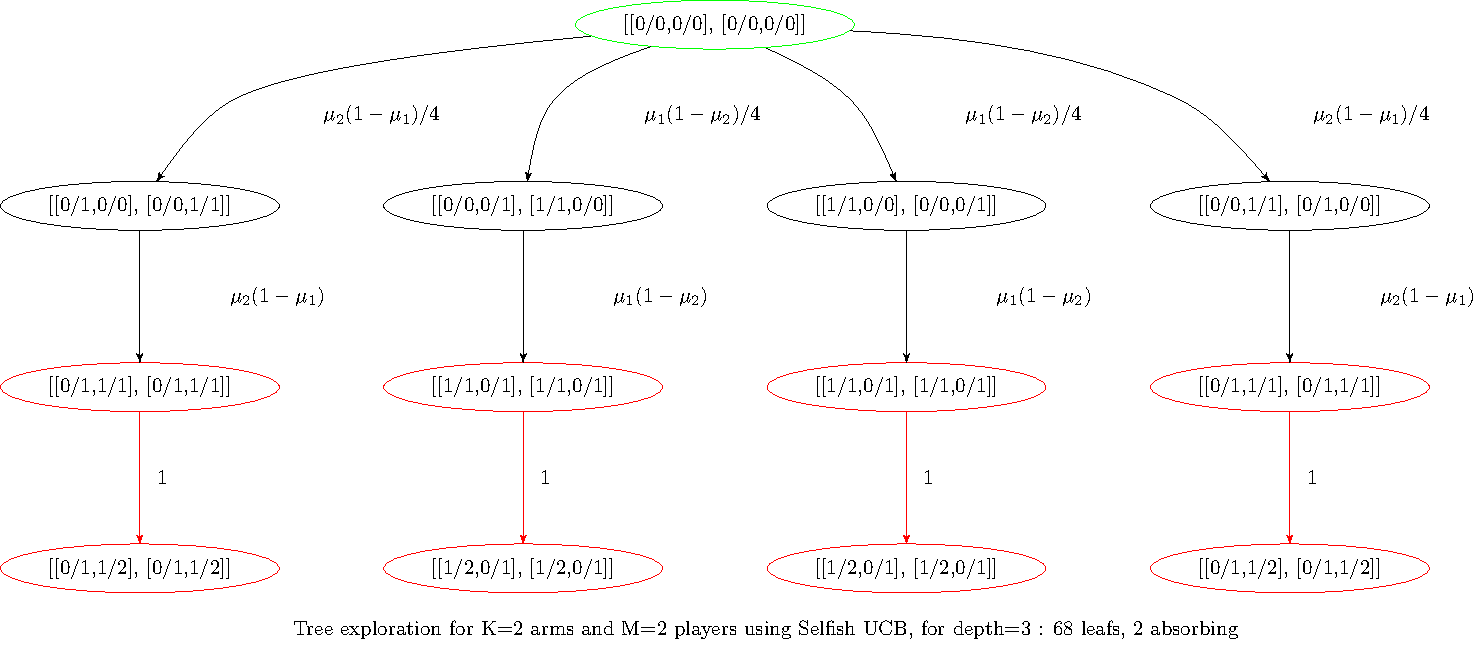
\includegraphics[width=0.70\textwidth]{2-Chapters/5-Chapter/ALT_2018__MPBandits.git/figures/Tree_exploration_K=2_M=2_depth=3__Selfish_UCB__absorbing.pdf}
%     % 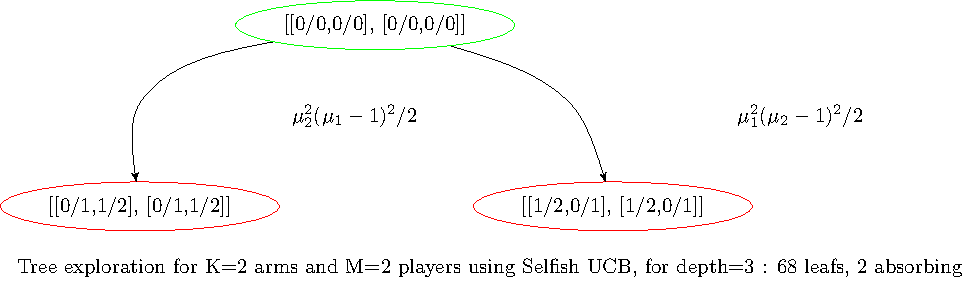
\includegraphics[width=0.70\textwidth]{Tree_exploration_K=2_M=2_depth=3__Selfish_UCB__absorbing__leafs.pdf}
%     % 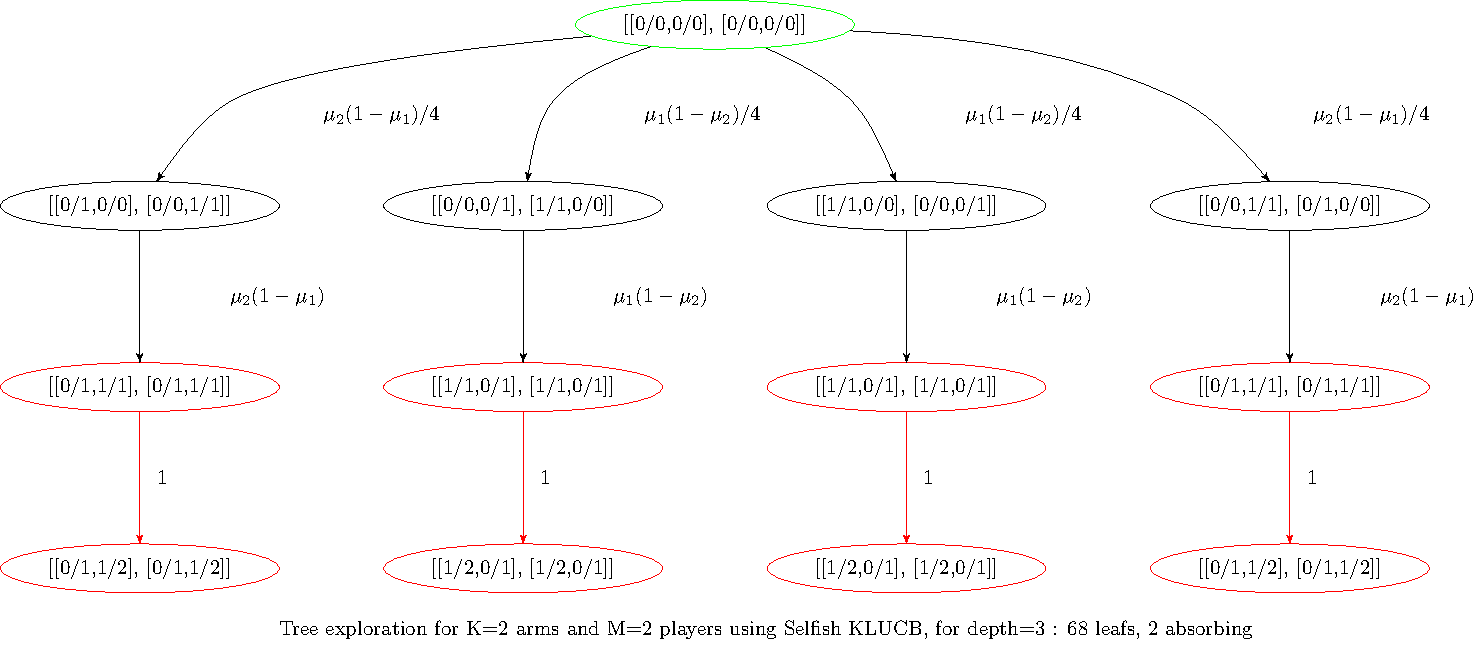
\includegraphics[width=0.70\textwidth]{Tree_exploration_K=2_M=2_depth=3__Selfish_KLUCB__absorbing.pdf}
%     % 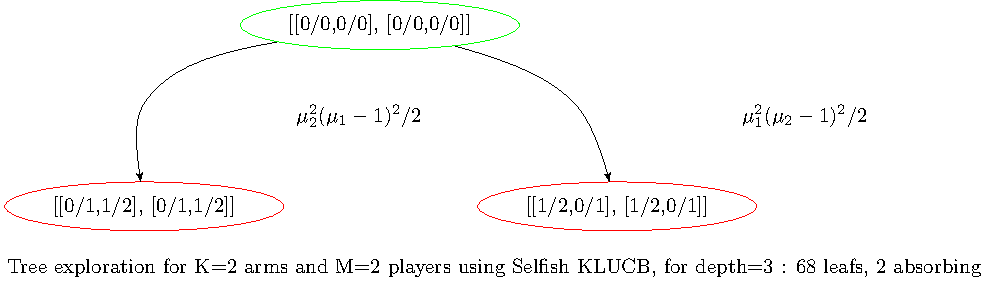
\includegraphics[width=0.70\textwidth]{Tree_exploration_K=2_M=2_depth=3__Selfish_KLUCB__absorbing__leafs.pdf}
%     \caption[Trajectories of $M=2$ players using \Selfish-\UCB{} for $K=2$ arms.]{For $K=2$ arms and $M=2$ players using \Selfish-\UCB, for depth$=3$: $2$ \textbf{\textcolor{red}{absorbing configurations}}. Each rectangle represents a configuration, as the matrix $[[\widetilde{S_k}^j(t) / T_k^j(t) ]_j]_k$. Absorbing configurations from depth $2$ are case of equality of the two vectors and the \Selfish{} indices $\widetilde{U_k}^j(t)$. Transitions are labeled with their probabilities.}
%     \label{fig:5:oneGameTree_SelfishKLUCB}
% \end{figure}

% From the structure of such game tree, we conjecture that the probability of reaching absorbing configurations (before a certain time $t$) is always lower-bounded
% by a polynomial function of $\mu_1,\dots,\mu_K$ and $1-\mu_1,\dots,1-\mu_K$,
% of degree at most $t$ in each variable.
% % with coefficients smaller than $1$.
% % and without simple factors (\ie, $\mu_k^d$).
% %
% As such, the lower bound on probability of failures should decrease when $K$ and $M$ increase, and this is coherent with the experiments for $K=9$ or $K=17$ (see Figures~\ref{fig:5:MP__K9_M2-6-9_T10000_N200__4_algos} and \ref{fig:5:MP__K17_M6-12-17_T10000_N100__4_algos}),
% where \Selfish{} is shown to be uniformly more efficient than \rhoRand.
% %
% Of course, one cannot run an infinite number of simulations, and the smaller the probability of failure, the less likely it is to observe a failure
% in a finite number of runs.

% % IDEA
% \paragraph{Ideas to fix \Selfish{} ?}
% %
% It could be possible to change the \Selfish{} algorithm to add a way to escape such absorbing trajectories.
% For instance one could imagine that after seen seeing, \eg, $x=10$ collisions in a row,
% a certain random action could be taken by the players.
% These tricks can work empirically in some cases,
% but they are harder to analyze formally,
% and it is hard to tune the parameters (here $x$, but possibly more),
% and we do not find such tricks to be promising from a theoretical point-of-view.



% -----------------------------------------------------------------
% -----------------------------------------------------------------
% \subsection{Additional figures}
\label{app:5:moreplots}

% We include here plots missing from Section~\ref{sec:5:experiments},
% and some additional numerical results.


% -----------------------------------------------------------------
\subsection*{Illustrating the lower bound}
\label{app:5:illustrationLowerBound}

% \TODOL{Maybe we can not include this part and just points to the paper \cite{Besson2018ALT}?}

We proved in Theorem~\ref{thm:5:BetterLowerBound} that the normalized regret, \ie, $R_T$ divided by
$\log T$, is asymptotically lower bounded by a constant $C_{\boldsymbol{\mu}, M}$
depending on the problem $\boldsymbol{\mu}$ and the number of players $M$, for any $\cA$.
\begin{equation}
  \mathop{\lim\inf}\limits_{T \to +\infty} \frac{R_T(\boldsymbol{\mu}, M, \cA)}{\log T} \geq C_{\boldsymbol{\mu}, M}.
\end{equation}
%
For an example problem with $K = 9$ arms, we display below on the $x$ axis is
the number of player, from $1$ player to $9$ players, and on the
$y$ axis is the value of this constant $C_{\boldsymbol{\mu}, M}$, from the initial
theorem and from our theorem.
We chose a simple problem, with Bernoulli
distributed arms, with $\boldsymbol{\mu} = [0.1, 0.2, \dots, 0.9]$.
% (as used in some articles).
%
Figure~\ref{fig:5:CompLowerBounds} clearly shows that our improved lower bound is indeed larger than the initial one by \cite{Zhao10},
and both become uninformative when $M=K$ (\ie, it gives $R_T / \log(T) \geq 0$ which is obvious anyway).

\begin{figure}[h!]
  \centering
  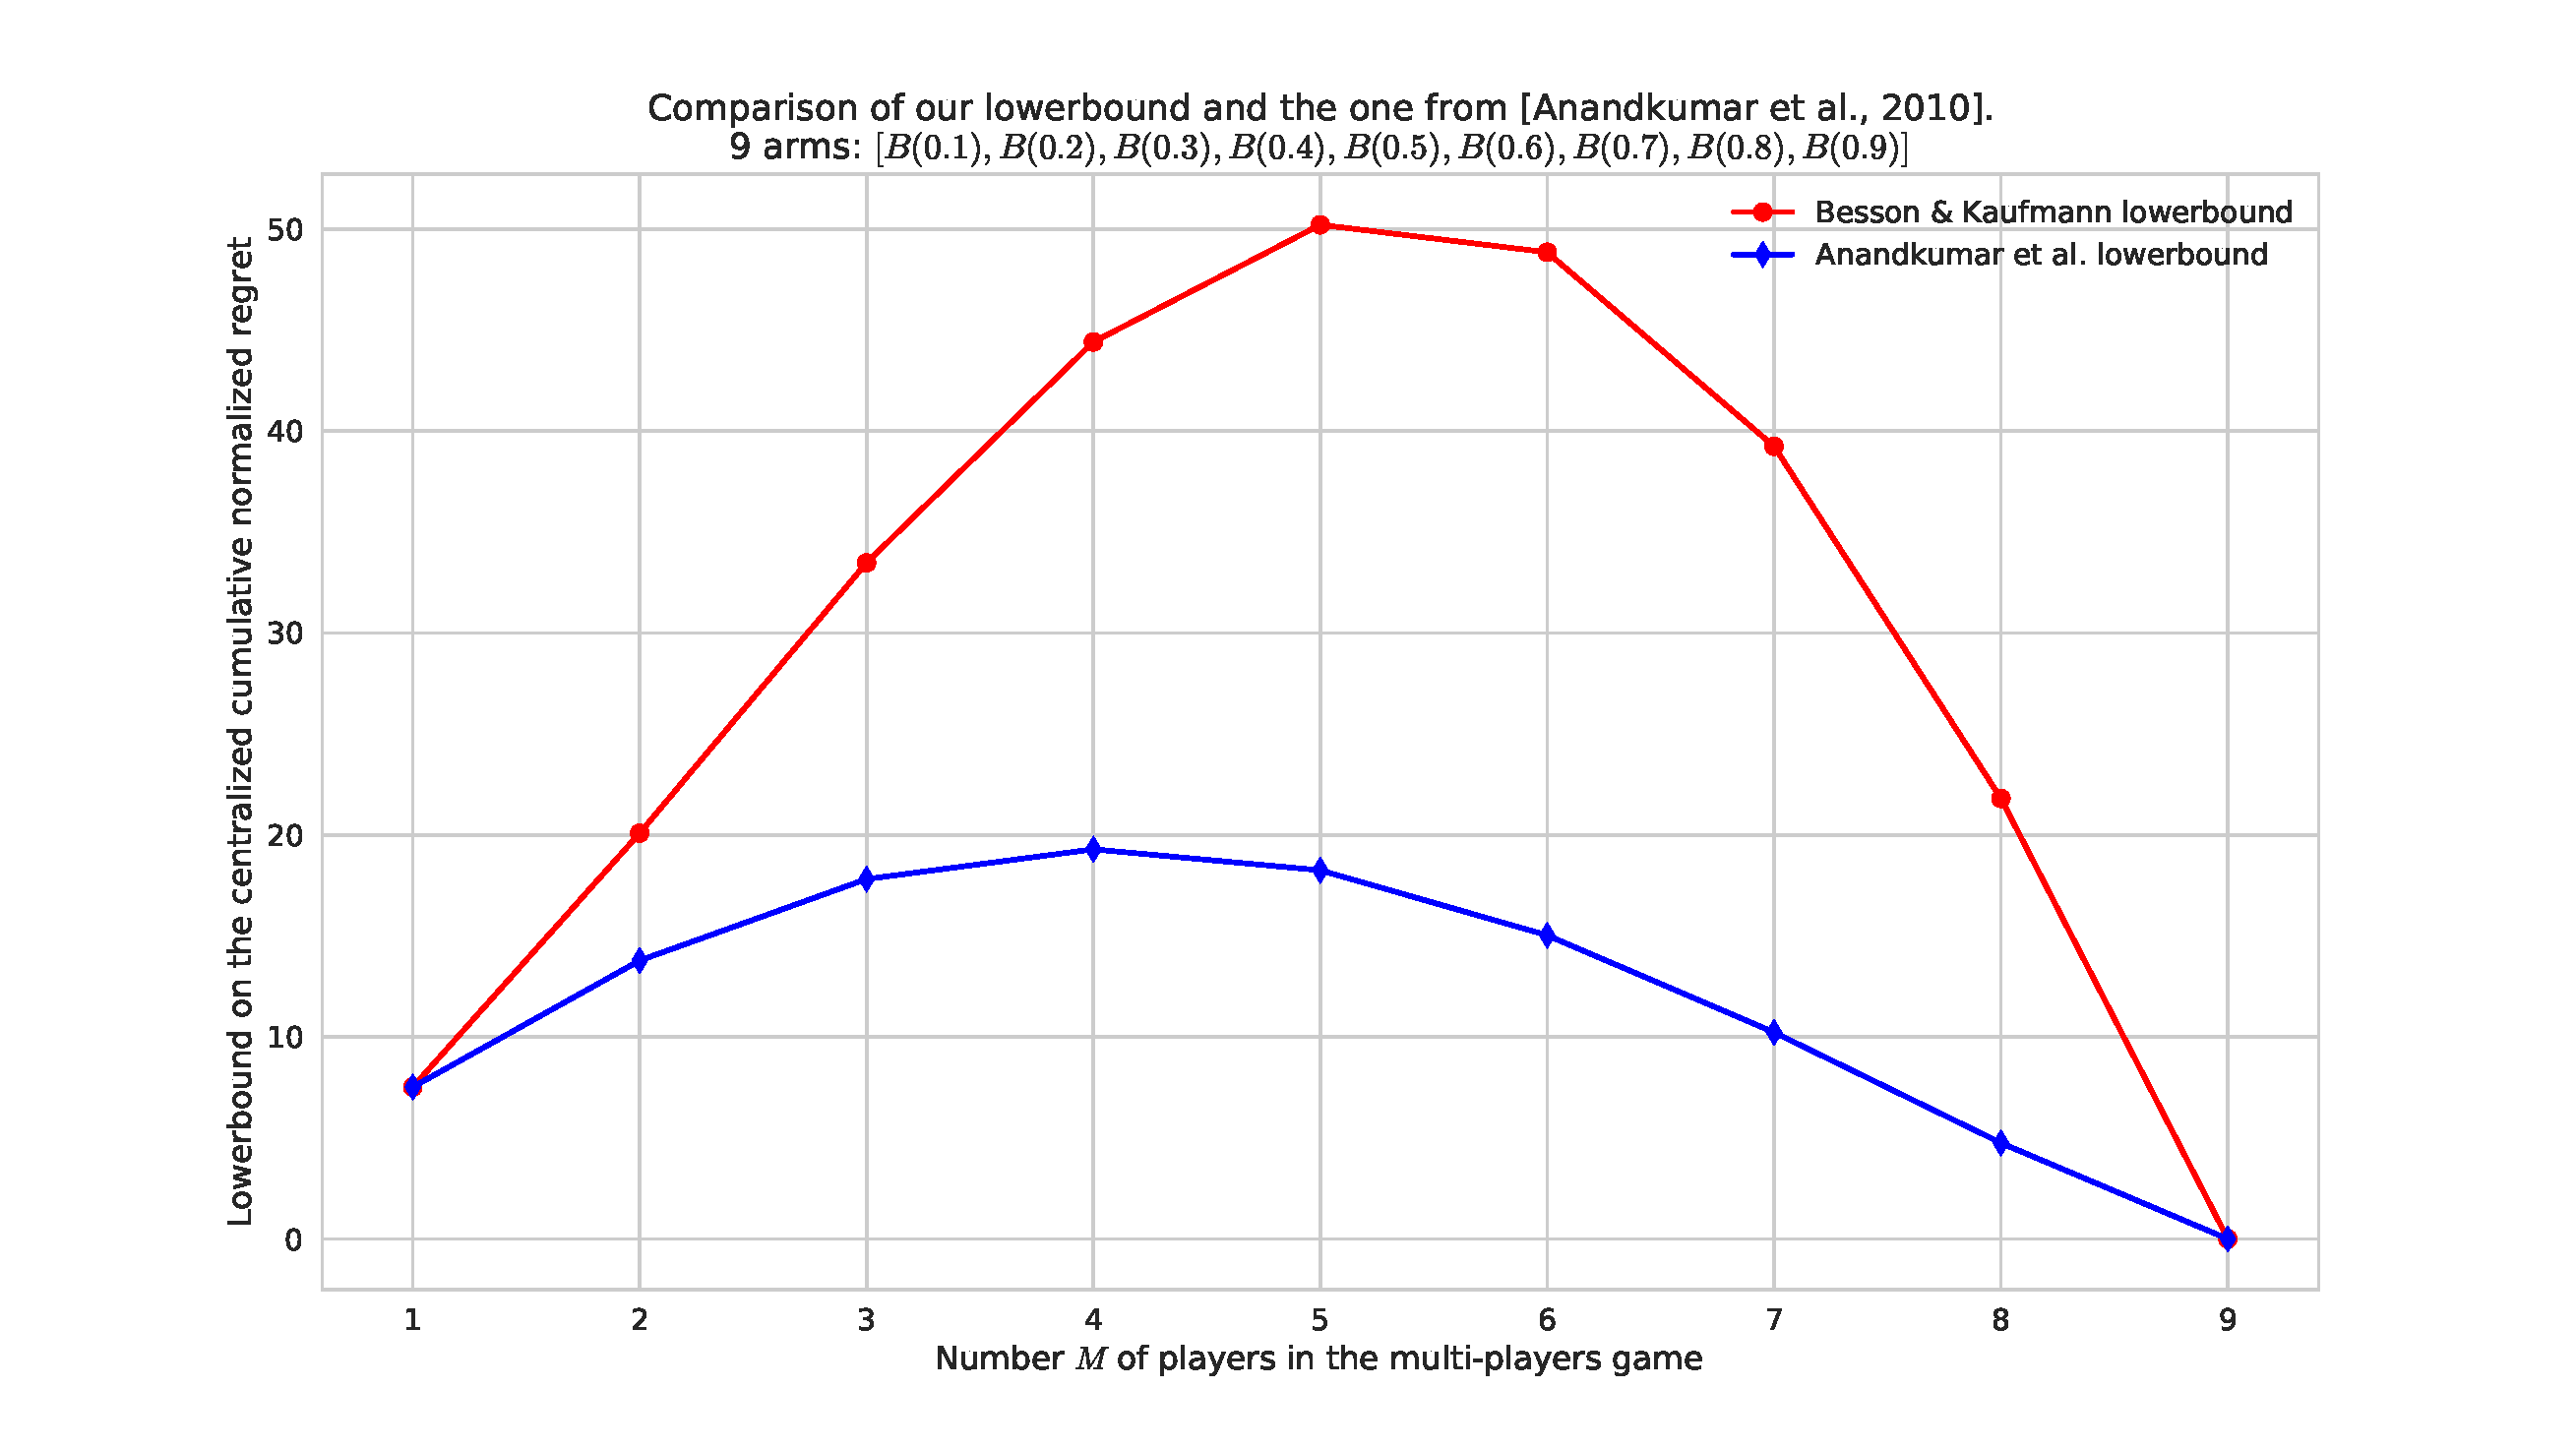
\includegraphics[width=0.95\textwidth]{Comparison_of_our_lowerbound_and_Anandkumar_2010__9_arms.pdf}
  \caption[Comparison of our lower bound against the one from \cite{Zhao10}]{Comparison of our lower bound against the one from \cite{Zhao10}, on a simple problem with $9$ Bernoulli arms, of means $\boldsymbol{\mu} = [0.1, 0.2, \dots, 0.9]$, as a function of the number of players $M$.}
  \label{fig:5:CompLowerBounds}
\end{figure}




% -----------------------------------------------------------------
\subsection*{Illustrating the regret decomposition}
\label{app:5:illustrationRegretDecomposition}

The Figure~\ref{fig:5:MP__M9_K9_T10000_N1000__9_algos__main_RegretCentralized____env6} below
shows the regret $R_T(\boldsymbol{\mu}, M, \cA)$
on the same example problem $\boldsymbol{\mu}$, with $K = 9$ arms and respectively $M = 6$, or $9$ players, for \Selfish-\klUCB.
%
It is just a simple way to check that the two lower bounds on the regret indeed appear as valid lower bounds empirically,
and are moreover lower bounds on the count of selections (\ref{eq:5:term1}, displayed in \textcolor{blue}{cyan}).
%
The lower bounds (in black) are $C(\boldsymbol{\mu}, M) \log t$, the dashed line
for the lower bound from \cite{Zhao10}, and the continuous line is our lower bound.
%
These plot show the regret (in red),
% the three lower bounds
% (centralized, \citeauthor{Anandkumar11}'s and our lower bounds, in black),
and the three terms \ref{eq:5:term1}, \ref{eq:5:term2}, \ref{eq:5:term3} in the decomposition of the regret.
As explained in Lemma~\ref{lem:5:DecompositionRegret}, term \ref{eq:5:term2} is not always non-negative.
For $M=9$ and \Selfish, \ref{eq:5:term3} is actually larger than the regret,
and term \ref{eq:5:term1} is zero, as well as the lower bounds.


%
% System regret and three terms
%
\begin{figure}[!h]
    \centering
    % \begin{subfigure}[!h]{1.00\textwidth}
        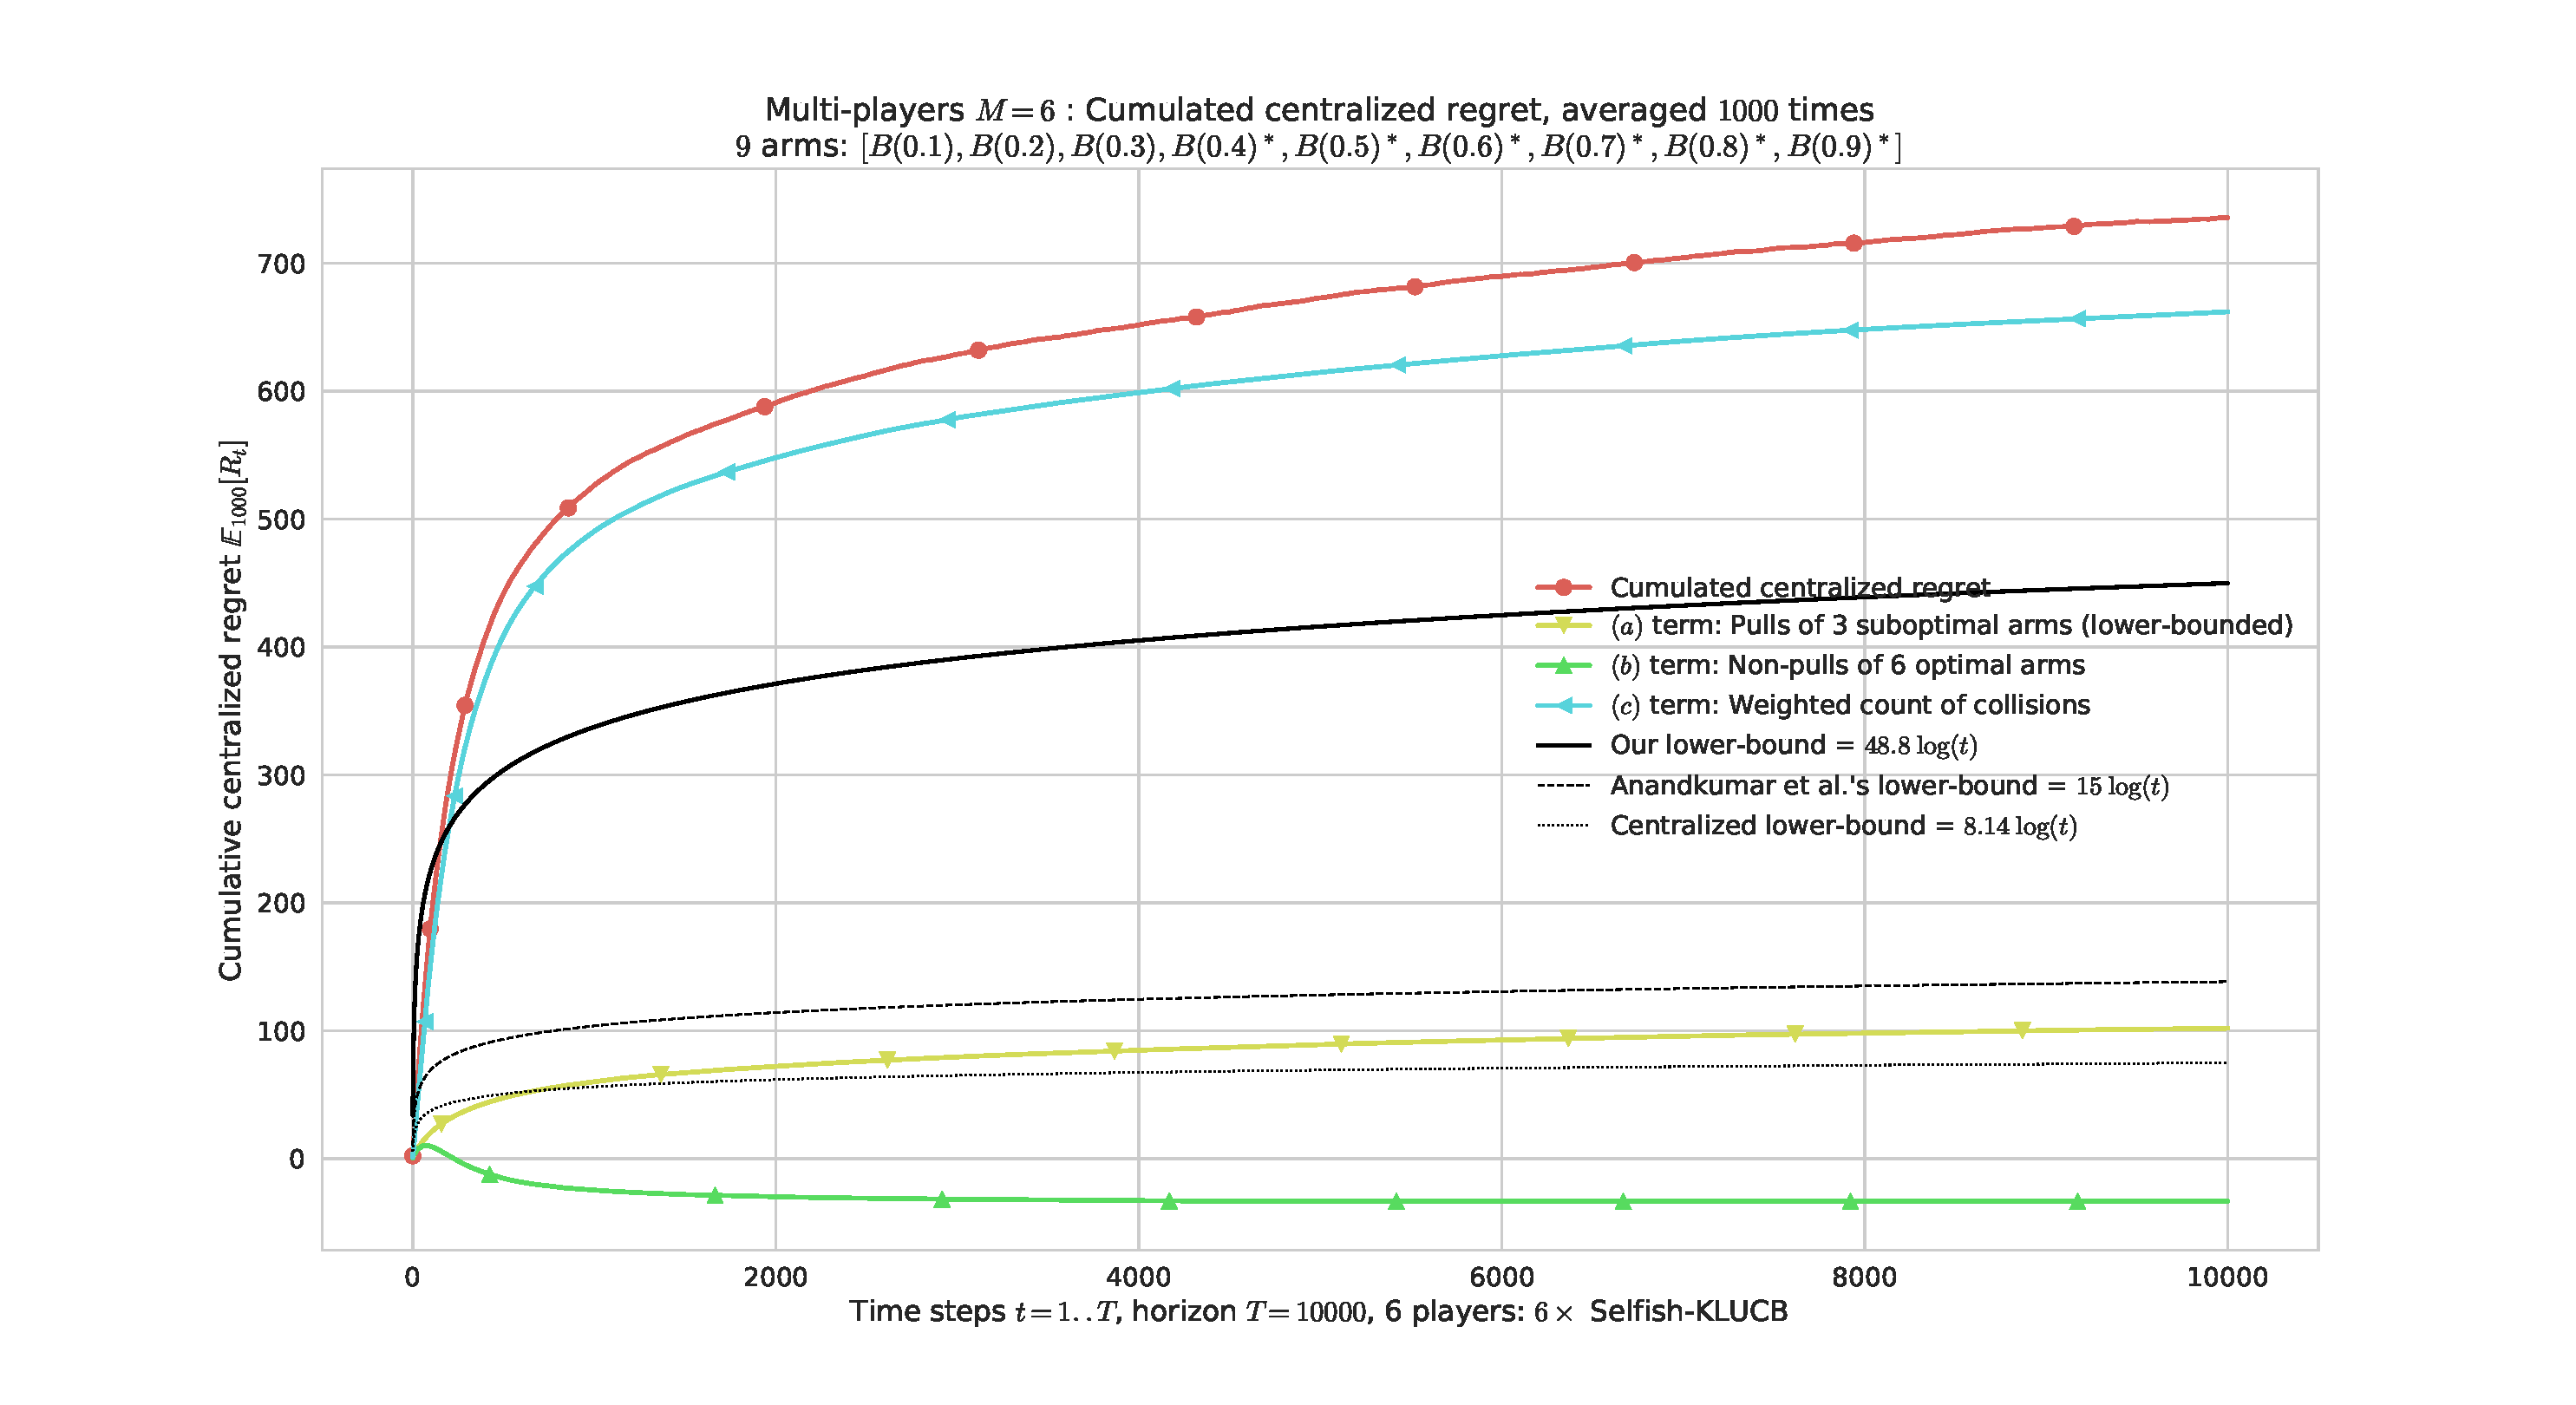
\includegraphics[width=1.00\textwidth]{main_RegretCentralized____env4-4_2092905764868974160.pdf}
    % \end{subfigure}
    % ~
    % \begin{subfigure}[!h]{1.00\textwidth}
        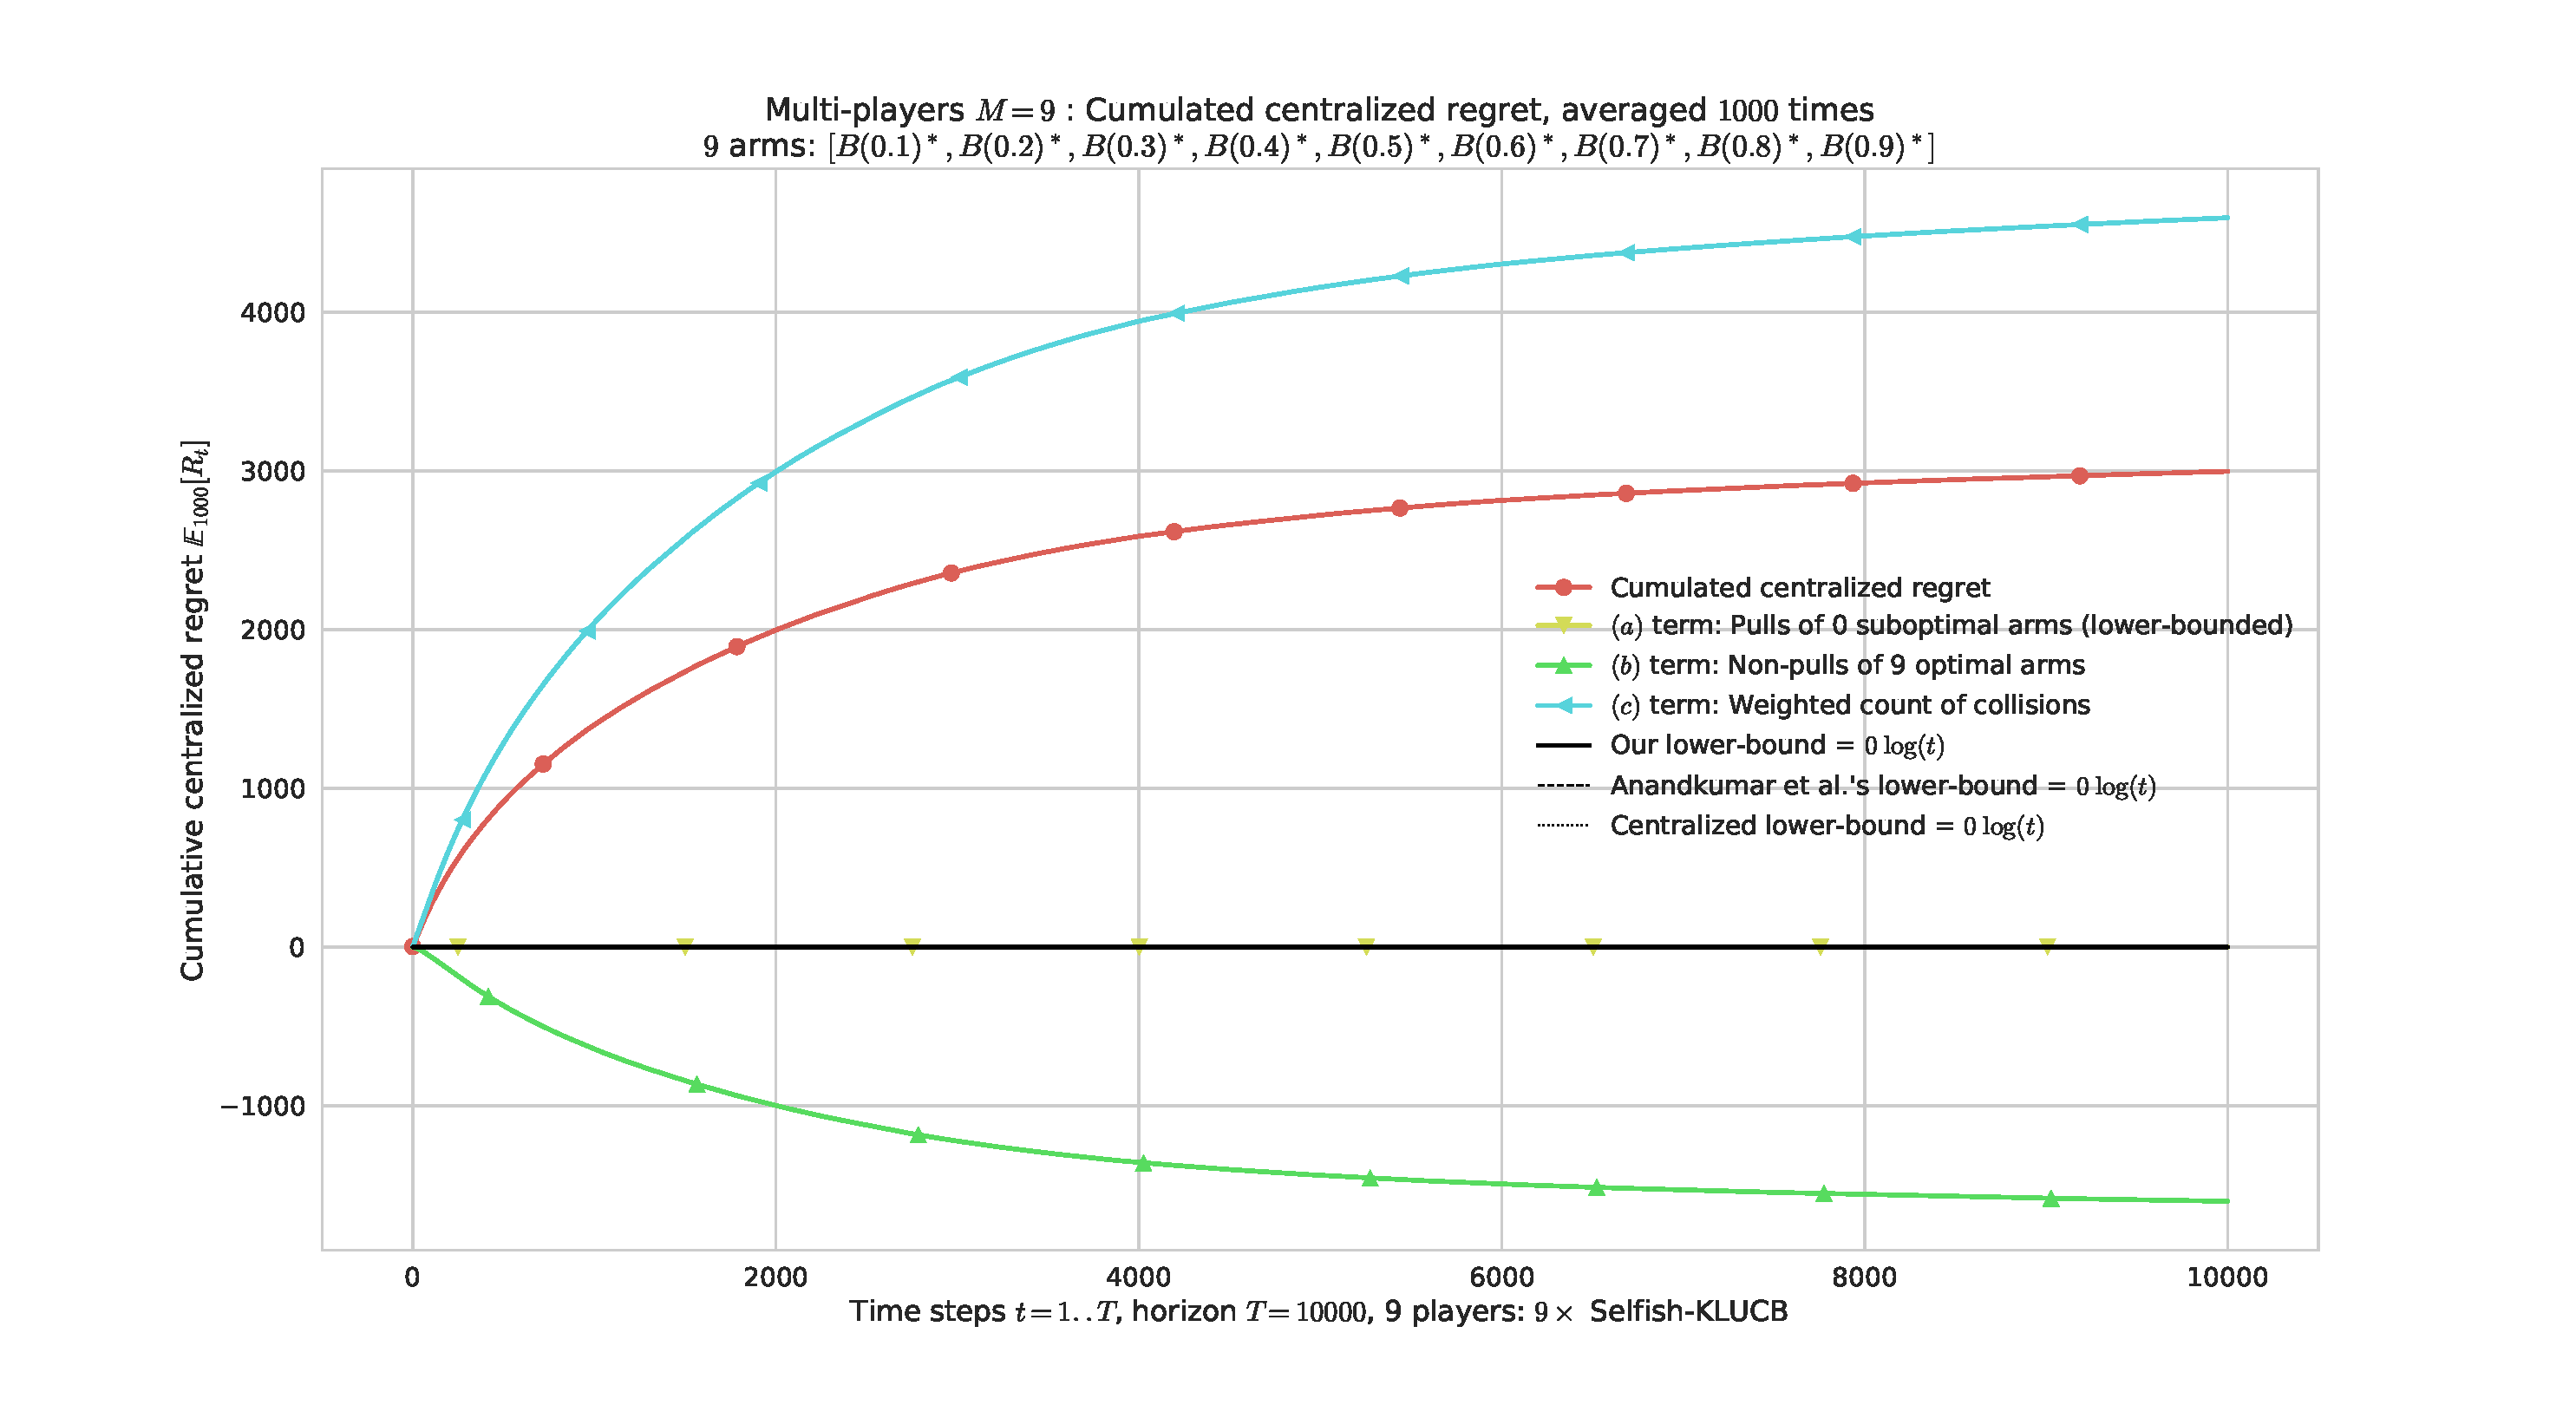
\includegraphics[width=1.00\textwidth]{main_RegretCentralized____env4-4_1699475021767911583.pdf}
    % \end{subfigure}
    \caption[Illustrating the decomposition of the multi-player regret with its three terms]{The three terms \ref{eq:5:term1}, \ref{eq:5:term2}, \ref{eq:5:term3} of the multi-player regret, and lower bounds \eqref{eq:5:ourLowerBound} and \eqref{eq:5:Zhao10LowerBound} in \textbf{black}, for \Selfish-\klUCB: $M=6$ and $M=9$ players, $K=9$ arms, horizon $T=10000$ (for $1000$ runs).}
    \label{fig:5:MP__M9_K9_T10000_N1000__9_algos__main_RegretCentralized____env6}
    % \vspace*{-15pt}  % XXX remove if problem
\end{figure}


% \subsubsection{Figures from Section~\ref{sec:5:experiments}}
% \label{app:5:plotsFromSec5}

% This last Appendix includes the figures used in Section~\ref{sec:5:experiments},
% with additional comments.


